\renewcommand{\imagepath}{../30-mot/img}

\chapter{The 3-dimensional Magneto-optical Trap}

\todo{TODO: make spectroscopic notation non-italic}
In the first section of this chapter, the theory of laser cooling with magneto-optical traps and gray molasses is outlined. Subsequently, the geometry, the laser setup, the optics and the magnetic gradients for the 3-dimensional magneto-optical trap in the FermiQP demonstrator will be presented. Finally, estimations of important parameters of the magneto-optical trap will be given.

Due to massive supply chain problems and delivery time extensions by part vendors, only the laser setup and the magnetic gradient coils could be assembled and characterized during the writing of the thesis. For the other aspects of the trap, details of planning and simulations are presented.
\todo{more precise,Make clear what is done already and what is still outstanding}

\section{Theory of Laser Cooling with Magneto-optical Traps and Gray Molasses}
\todo{History (Haensch, Earnshaw), examples, Nobel Prize 1997.}

Laser light exerting a force onto an atom is the underlying mechanism of laser cooling. There are different implementations of laser cooling, each one making use of a different way light can interact with atoms: Doppler-cooling techniques on the one hand, as e.g.\ used in magneto-optical traps, are limited by the spontaneous decay of excited states regarding the achievable temperature. Sub-Doppler-cooling techniques, on the other hand, circumvent this limit using a variety atom-light interactions, such as the optical dipole trap, Raman sideband cooling or Sisyphus cooling~\cite{foot_atomic_2005}.

The rest of this section is covering the theory of magneto-optical traps and the implementation of the 3-dimensional magneto-optical trap of the FermiQP demonstrator experiment. The explanations closely follow the respective chapters in~\cite{foot_atomic_2005} and~\cite{metcalf_laser_1999}.

\subsection*{Light scattering on atoms}
Electromagnetic waves carry momentum $\vec p = \hbar k$, which is directed into their propagation direction and depends on their wavelength $\lambda = \frac{2\pi}{k}$. When laser light scatters on atoms, a momentum transfer between the photons of the laser and the atoms takes place. The total transfer can be broken down into two parts: the absorption of laser photons where the atoms acquire momentum $\hbar \vec k$ per photon, and the spontaneous emission of photons where the atoms lose $\hbar \vec k_\text{emitted}$ per photon:
\begin{align}
    \vec p_\text{after} &= \vec p_\text{before} + \hbar \vec k + \hbar \vec k_\text{emitted}
\end{align}
The latter, however, averages to zero over many scattering events as photons are emitted into random directions. In this way, atoms loose momentum over many scattering events, if the propagation of the light and the atom movement are in opposite directions:
\begin{align}
    \Braket{\vec p_\text{after} - \vec p_\text{before}} = \Braket{\hbar \vec k} + \underbrace{\Braket{\hbar \vec k_\text{emitted}}}_{=0}
\end{align}
As visualized in figure~\ref{fig:light_scattering_momentum_transfer}, the atoms are decelerated opposite the direction of laser propagation, corresponding to cooling of the atoms.

\begin{figure}    
    \centering
    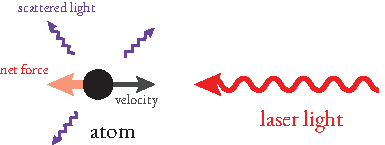
\includegraphics[]{\imagepath/light_scattering_momentum_transfer/light_scattering_momentum_transfer.pdf}
    \caption{Schematic of momentum transfer from the laser against the atom movement direction. The momenta of the scattered photons, originating from spontaneous in random directions, averages to zero.}\label{fig:light_scattering_momentum_transfer}
\end{figure}

The rate at which this happens is determined by the fraction $\rho_{ee}$ of atoms in the excited state when light of wavelength $\omega_\text{laser}$ and intensity $I$ is shone in:
\begin{align}
    R_\text{scatter} = \Gamma \rho_{ee}
\end{align}
with the rate $\Gamma$ of spontaneous decays from the excited state into the ground state. The scattering force which corresponds to the decrease of momentum of the atoms is hence
\begin{align}
    \vec F_\text{scatter} = R_\text{scatter} \hbar \vec k = \Gamma \rho_{ee} \hbar \vec k.
\end{align}

The light-atom interaction process can be described semi-classically understanding the light as a classical electromagnetic wave, but describing the dynamics within the atom using the quantum mechanical optical Bloch equations, according to which the steady-state population of the excited state amounts to
\begin{align}
    \rho_{ee} = \frac{s_0/2}{1 + s_0 + {\left(\frac{2\delta}{\Gamma}\right)}^2},
\end{align}
with the saturation parameter $s_0 = \frac{I}{I_\text{s}} = \frac{2\Omega^2}{\Gamma^2}$, the Rabi frequency $\Omega \propto \sqrt{I}$, and the detuning $\delta$. The detuning is the deviation of the laser frequency from the transition frequency, as seen by the atom considering the Doppler shift stemming from its velocity $\vec v$ with respect to the propagation direction $\vec k$ of the laser:
\begin{align}
    \delta &= \overbrace{\omega_\text{laser} - \vec k \vec v }^\text{apparent laser frequency}- \omega_\text{transition} \\
    \nonumber & = \omega_\text{laser}  - \omega_\text{transition} \pm kv \cos \theta
\end{align}
where $+$ is for atoms moving against and $-$ for atoms moving along with the laser. $\theta$ is the  angle between the atoms' velocity and the propagation direction of the light.

\begin{figure}
    \centering
    \begin{pgfpicture}
        \pgftext{%% Creator: Matplotlib, PGF backend
%%
%% To include the figure in your LaTeX document, write
%%   \input{<filename>.pgf}
%%
%% Make sure the required packages are loaded in your preamble
%%   \usepackage{pgf}
%%
%% Also ensure that all the required font packages are loaded; for instance,
%% the lmodern package is sometimes necessary when using math font.
%%   \usepackage{lmodern}
%%
%% Figures using additional raster images can only be included by \input if
%% they are in the same directory as the main LaTeX file. For loading figures
%% from other directories you can use the `import` package
%%   \usepackage{import}
%%
%% and then include the figures with
%%   \import{<path to file>}{<filename>.pgf}
%%
%% Matplotlib used the following preamble
%%   \usepackage{fontspec}
%%   \setmainfont{DejaVuSerif.ttf}[Path=\detokenize{/usr/local/lib/python3.8/dist-packages/matplotlib/mpl-data/fonts/ttf/}]
%%   \setsansfont{DejaVuSans.ttf}[Path=\detokenize{/usr/local/lib/python3.8/dist-packages/matplotlib/mpl-data/fonts/ttf/}]
%%   \setmonofont{DejaVuSansMono.ttf}[Path=\detokenize{/usr/local/lib/python3.8/dist-packages/matplotlib/mpl-data/fonts/ttf/}]
%%
\begingroup%
\makeatletter%
\begin{pgfpicture}%
\pgfpathrectangle{\pgfpointorigin}{\pgfqpoint{3.727750in}{2.089021in}}%
\pgfusepath{use as bounding box, clip}%
\begin{pgfscope}%
\pgfsetbuttcap%
\pgfsetmiterjoin%
\pgfsetlinewidth{0.000000pt}%
\definecolor{currentstroke}{rgb}{1.000000,1.000000,1.000000}%
\pgfsetstrokecolor{currentstroke}%
\pgfsetstrokeopacity{0.000000}%
\pgfsetdash{}{0pt}%
\pgfpathmoveto{\pgfqpoint{0.000000in}{-0.000000in}}%
\pgfpathlineto{\pgfqpoint{3.727750in}{-0.000000in}}%
\pgfpathlineto{\pgfqpoint{3.727750in}{2.089021in}}%
\pgfpathlineto{\pgfqpoint{0.000000in}{2.089021in}}%
\pgfpathlineto{\pgfqpoint{0.000000in}{-0.000000in}}%
\pgfpathclose%
\pgfusepath{}%
\end{pgfscope}%
\begin{pgfscope}%
\pgfsetbuttcap%
\pgfsetmiterjoin%
\definecolor{currentfill}{rgb}{1.000000,1.000000,1.000000}%
\pgfsetfillcolor{currentfill}%
\pgfsetlinewidth{0.000000pt}%
\definecolor{currentstroke}{rgb}{0.000000,0.000000,0.000000}%
\pgfsetstrokecolor{currentstroke}%
\pgfsetstrokeopacity{0.000000}%
\pgfsetdash{}{0pt}%
\pgfpathmoveto{\pgfqpoint{0.576569in}{0.499970in}}%
\pgfpathlineto{\pgfqpoint{3.627750in}{0.499970in}}%
\pgfpathlineto{\pgfqpoint{3.627750in}{1.986190in}}%
\pgfpathlineto{\pgfqpoint{0.576569in}{1.986190in}}%
\pgfpathlineto{\pgfqpoint{0.576569in}{0.499970in}}%
\pgfpathclose%
\pgfusepath{fill}%
\end{pgfscope}%
\begin{pgfscope}%
\pgfpathrectangle{\pgfqpoint{0.576569in}{0.499970in}}{\pgfqpoint{3.051181in}{1.486220in}}%
\pgfusepath{clip}%
\pgfsetbuttcap%
\pgfsetmiterjoin%
\definecolor{currentfill}{rgb}{1.000000,0.000000,0.000000}%
\pgfsetfillcolor{currentfill}%
\pgfsetlinewidth{0.401500pt}%
\definecolor{currentstroke}{rgb}{1.000000,0.000000,0.000000}%
\pgfsetstrokecolor{currentstroke}%
\pgfsetdash{}{0pt}%
\pgfpathmoveto{\pgfqpoint{2.422214in}{1.895735in}}%
\pgfpathlineto{\pgfqpoint{2.443551in}{1.918635in}}%
\pgfpathlineto{\pgfqpoint{2.443551in}{1.898025in}}%
\pgfpathlineto{\pgfqpoint{2.742268in}{1.898025in}}%
\pgfpathlineto{\pgfqpoint{2.742268in}{1.893445in}}%
\pgfpathlineto{\pgfqpoint{2.443551in}{1.893445in}}%
\pgfpathlineto{\pgfqpoint{2.443551in}{1.872835in}}%
\pgfpathlineto{\pgfqpoint{2.422214in}{1.895735in}}%
\pgfpathclose%
\pgfusepath{stroke,fill}%
\end{pgfscope}%
\begin{pgfscope}%
\pgfpathrectangle{\pgfqpoint{0.576569in}{0.499970in}}{\pgfqpoint{3.051181in}{1.486220in}}%
\pgfusepath{clip}%
\pgfsetbuttcap%
\pgfsetmiterjoin%
\definecolor{currentfill}{rgb}{1.000000,0.000000,0.000000}%
\pgfsetfillcolor{currentfill}%
\pgfsetlinewidth{0.401500pt}%
\definecolor{currentstroke}{rgb}{1.000000,0.000000,0.000000}%
\pgfsetstrokecolor{currentstroke}%
\pgfsetdash{}{0pt}%
\pgfpathmoveto{\pgfqpoint{3.062322in}{1.895735in}}%
\pgfpathlineto{\pgfqpoint{3.040985in}{1.872835in}}%
\pgfpathlineto{\pgfqpoint{3.040985in}{1.893445in}}%
\pgfpathlineto{\pgfqpoint{2.742268in}{1.893445in}}%
\pgfpathlineto{\pgfqpoint{2.742268in}{1.898025in}}%
\pgfpathlineto{\pgfqpoint{3.040985in}{1.898025in}}%
\pgfpathlineto{\pgfqpoint{3.040985in}{1.918635in}}%
\pgfpathlineto{\pgfqpoint{3.062322in}{1.895735in}}%
\pgfpathclose%
\pgfusepath{stroke,fill}%
\end{pgfscope}%
\begin{pgfscope}%
\pgfpathrectangle{\pgfqpoint{0.576569in}{0.499970in}}{\pgfqpoint{3.051181in}{1.486220in}}%
\pgfusepath{clip}%
\pgfsetrectcap%
\pgfsetroundjoin%
\pgfsetlinewidth{0.803000pt}%
\definecolor{currentstroke}{rgb}{0.690196,0.690196,0.690196}%
\pgfsetstrokecolor{currentstroke}%
\pgfsetdash{}{0pt}%
\pgfpathmoveto{\pgfqpoint{0.715259in}{0.499970in}}%
\pgfpathlineto{\pgfqpoint{0.715259in}{1.986190in}}%
\pgfusepath{stroke}%
\end{pgfscope}%
\begin{pgfscope}%
\pgfsetbuttcap%
\pgfsetroundjoin%
\definecolor{currentfill}{rgb}{0.000000,0.000000,0.000000}%
\pgfsetfillcolor{currentfill}%
\pgfsetlinewidth{0.803000pt}%
\definecolor{currentstroke}{rgb}{0.000000,0.000000,0.000000}%
\pgfsetstrokecolor{currentstroke}%
\pgfsetdash{}{0pt}%
\pgfsys@defobject{currentmarker}{\pgfqpoint{0.000000in}{-0.048611in}}{\pgfqpoint{0.000000in}{0.000000in}}{%
\pgfpathmoveto{\pgfqpoint{0.000000in}{0.000000in}}%
\pgfpathlineto{\pgfqpoint{0.000000in}{-0.048611in}}%
\pgfusepath{stroke,fill}%
}%
\begin{pgfscope}%
\pgfsys@transformshift{0.715259in}{0.499970in}%
\pgfsys@useobject{currentmarker}{}%
\end{pgfscope}%
\end{pgfscope}%
\begin{pgfscope}%
\definecolor{textcolor}{rgb}{0.000000,0.000000,0.000000}%
\pgfsetstrokecolor{textcolor}%
\pgfsetfillcolor{textcolor}%
\pgftext[x=0.715259in,y=0.402748in,,top]{\color{textcolor}\rmfamily\fontsize{9.000000}{10.800000}\selectfont \ensuremath{-}\ensuremath{8}}%
\end{pgfscope}%
\begin{pgfscope}%
\pgfpathrectangle{\pgfqpoint{0.576569in}{0.499970in}}{\pgfqpoint{3.051181in}{1.486220in}}%
\pgfusepath{clip}%
\pgfsetrectcap%
\pgfsetroundjoin%
\pgfsetlinewidth{0.803000pt}%
\definecolor{currentstroke}{rgb}{0.690196,0.690196,0.690196}%
\pgfsetstrokecolor{currentstroke}%
\pgfsetdash{}{0pt}%
\pgfpathmoveto{\pgfqpoint{1.141998in}{0.499970in}}%
\pgfpathlineto{\pgfqpoint{1.141998in}{1.986190in}}%
\pgfusepath{stroke}%
\end{pgfscope}%
\begin{pgfscope}%
\pgfsetbuttcap%
\pgfsetroundjoin%
\definecolor{currentfill}{rgb}{0.000000,0.000000,0.000000}%
\pgfsetfillcolor{currentfill}%
\pgfsetlinewidth{0.803000pt}%
\definecolor{currentstroke}{rgb}{0.000000,0.000000,0.000000}%
\pgfsetstrokecolor{currentstroke}%
\pgfsetdash{}{0pt}%
\pgfsys@defobject{currentmarker}{\pgfqpoint{0.000000in}{-0.048611in}}{\pgfqpoint{0.000000in}{0.000000in}}{%
\pgfpathmoveto{\pgfqpoint{0.000000in}{0.000000in}}%
\pgfpathlineto{\pgfqpoint{0.000000in}{-0.048611in}}%
\pgfusepath{stroke,fill}%
}%
\begin{pgfscope}%
\pgfsys@transformshift{1.141998in}{0.499970in}%
\pgfsys@useobject{currentmarker}{}%
\end{pgfscope}%
\end{pgfscope}%
\begin{pgfscope}%
\definecolor{textcolor}{rgb}{0.000000,0.000000,0.000000}%
\pgfsetstrokecolor{textcolor}%
\pgfsetfillcolor{textcolor}%
\pgftext[x=1.141998in,y=0.402748in,,top]{\color{textcolor}\rmfamily\fontsize{9.000000}{10.800000}\selectfont \ensuremath{-}\ensuremath{6}}%
\end{pgfscope}%
\begin{pgfscope}%
\pgfpathrectangle{\pgfqpoint{0.576569in}{0.499970in}}{\pgfqpoint{3.051181in}{1.486220in}}%
\pgfusepath{clip}%
\pgfsetrectcap%
\pgfsetroundjoin%
\pgfsetlinewidth{0.803000pt}%
\definecolor{currentstroke}{rgb}{0.690196,0.690196,0.690196}%
\pgfsetstrokecolor{currentstroke}%
\pgfsetdash{}{0pt}%
\pgfpathmoveto{\pgfqpoint{1.568737in}{0.499970in}}%
\pgfpathlineto{\pgfqpoint{1.568737in}{1.986190in}}%
\pgfusepath{stroke}%
\end{pgfscope}%
\begin{pgfscope}%
\pgfsetbuttcap%
\pgfsetroundjoin%
\definecolor{currentfill}{rgb}{0.000000,0.000000,0.000000}%
\pgfsetfillcolor{currentfill}%
\pgfsetlinewidth{0.803000pt}%
\definecolor{currentstroke}{rgb}{0.000000,0.000000,0.000000}%
\pgfsetstrokecolor{currentstroke}%
\pgfsetdash{}{0pt}%
\pgfsys@defobject{currentmarker}{\pgfqpoint{0.000000in}{-0.048611in}}{\pgfqpoint{0.000000in}{0.000000in}}{%
\pgfpathmoveto{\pgfqpoint{0.000000in}{0.000000in}}%
\pgfpathlineto{\pgfqpoint{0.000000in}{-0.048611in}}%
\pgfusepath{stroke,fill}%
}%
\begin{pgfscope}%
\pgfsys@transformshift{1.568737in}{0.499970in}%
\pgfsys@useobject{currentmarker}{}%
\end{pgfscope}%
\end{pgfscope}%
\begin{pgfscope}%
\definecolor{textcolor}{rgb}{0.000000,0.000000,0.000000}%
\pgfsetstrokecolor{textcolor}%
\pgfsetfillcolor{textcolor}%
\pgftext[x=1.568737in,y=0.402748in,,top]{\color{textcolor}\rmfamily\fontsize{9.000000}{10.800000}\selectfont \ensuremath{-}\ensuremath{4}}%
\end{pgfscope}%
\begin{pgfscope}%
\pgfpathrectangle{\pgfqpoint{0.576569in}{0.499970in}}{\pgfqpoint{3.051181in}{1.486220in}}%
\pgfusepath{clip}%
\pgfsetrectcap%
\pgfsetroundjoin%
\pgfsetlinewidth{0.803000pt}%
\definecolor{currentstroke}{rgb}{0.690196,0.690196,0.690196}%
\pgfsetstrokecolor{currentstroke}%
\pgfsetdash{}{0pt}%
\pgfpathmoveto{\pgfqpoint{1.995475in}{0.499970in}}%
\pgfpathlineto{\pgfqpoint{1.995475in}{1.986190in}}%
\pgfusepath{stroke}%
\end{pgfscope}%
\begin{pgfscope}%
\pgfsetbuttcap%
\pgfsetroundjoin%
\definecolor{currentfill}{rgb}{0.000000,0.000000,0.000000}%
\pgfsetfillcolor{currentfill}%
\pgfsetlinewidth{0.803000pt}%
\definecolor{currentstroke}{rgb}{0.000000,0.000000,0.000000}%
\pgfsetstrokecolor{currentstroke}%
\pgfsetdash{}{0pt}%
\pgfsys@defobject{currentmarker}{\pgfqpoint{0.000000in}{-0.048611in}}{\pgfqpoint{0.000000in}{0.000000in}}{%
\pgfpathmoveto{\pgfqpoint{0.000000in}{0.000000in}}%
\pgfpathlineto{\pgfqpoint{0.000000in}{-0.048611in}}%
\pgfusepath{stroke,fill}%
}%
\begin{pgfscope}%
\pgfsys@transformshift{1.995475in}{0.499970in}%
\pgfsys@useobject{currentmarker}{}%
\end{pgfscope}%
\end{pgfscope}%
\begin{pgfscope}%
\definecolor{textcolor}{rgb}{0.000000,0.000000,0.000000}%
\pgfsetstrokecolor{textcolor}%
\pgfsetfillcolor{textcolor}%
\pgftext[x=1.995475in,y=0.402748in,,top]{\color{textcolor}\rmfamily\fontsize{9.000000}{10.800000}\selectfont \ensuremath{-}\ensuremath{2}}%
\end{pgfscope}%
\begin{pgfscope}%
\pgfpathrectangle{\pgfqpoint{0.576569in}{0.499970in}}{\pgfqpoint{3.051181in}{1.486220in}}%
\pgfusepath{clip}%
\pgfsetrectcap%
\pgfsetroundjoin%
\pgfsetlinewidth{0.803000pt}%
\definecolor{currentstroke}{rgb}{0.690196,0.690196,0.690196}%
\pgfsetstrokecolor{currentstroke}%
\pgfsetdash{}{0pt}%
\pgfpathmoveto{\pgfqpoint{2.422214in}{0.499970in}}%
\pgfpathlineto{\pgfqpoint{2.422214in}{1.986190in}}%
\pgfusepath{stroke}%
\end{pgfscope}%
\begin{pgfscope}%
\pgfsetbuttcap%
\pgfsetroundjoin%
\definecolor{currentfill}{rgb}{0.000000,0.000000,0.000000}%
\pgfsetfillcolor{currentfill}%
\pgfsetlinewidth{0.803000pt}%
\definecolor{currentstroke}{rgb}{0.000000,0.000000,0.000000}%
\pgfsetstrokecolor{currentstroke}%
\pgfsetdash{}{0pt}%
\pgfsys@defobject{currentmarker}{\pgfqpoint{0.000000in}{-0.048611in}}{\pgfqpoint{0.000000in}{0.000000in}}{%
\pgfpathmoveto{\pgfqpoint{0.000000in}{0.000000in}}%
\pgfpathlineto{\pgfqpoint{0.000000in}{-0.048611in}}%
\pgfusepath{stroke,fill}%
}%
\begin{pgfscope}%
\pgfsys@transformshift{2.422214in}{0.499970in}%
\pgfsys@useobject{currentmarker}{}%
\end{pgfscope}%
\end{pgfscope}%
\begin{pgfscope}%
\definecolor{textcolor}{rgb}{0.000000,0.000000,0.000000}%
\pgfsetstrokecolor{textcolor}%
\pgfsetfillcolor{textcolor}%
\pgftext[x=2.422214in,y=0.402748in,,top]{\color{textcolor}\rmfamily\fontsize{9.000000}{10.800000}\selectfont \ensuremath{0}}%
\end{pgfscope}%
\begin{pgfscope}%
\pgfpathrectangle{\pgfqpoint{0.576569in}{0.499970in}}{\pgfqpoint{3.051181in}{1.486220in}}%
\pgfusepath{clip}%
\pgfsetrectcap%
\pgfsetroundjoin%
\pgfsetlinewidth{0.803000pt}%
\definecolor{currentstroke}{rgb}{0.690196,0.690196,0.690196}%
\pgfsetstrokecolor{currentstroke}%
\pgfsetdash{}{0pt}%
\pgfpathmoveto{\pgfqpoint{2.848952in}{0.499970in}}%
\pgfpathlineto{\pgfqpoint{2.848952in}{1.986190in}}%
\pgfusepath{stroke}%
\end{pgfscope}%
\begin{pgfscope}%
\pgfsetbuttcap%
\pgfsetroundjoin%
\definecolor{currentfill}{rgb}{0.000000,0.000000,0.000000}%
\pgfsetfillcolor{currentfill}%
\pgfsetlinewidth{0.803000pt}%
\definecolor{currentstroke}{rgb}{0.000000,0.000000,0.000000}%
\pgfsetstrokecolor{currentstroke}%
\pgfsetdash{}{0pt}%
\pgfsys@defobject{currentmarker}{\pgfqpoint{0.000000in}{-0.048611in}}{\pgfqpoint{0.000000in}{0.000000in}}{%
\pgfpathmoveto{\pgfqpoint{0.000000in}{0.000000in}}%
\pgfpathlineto{\pgfqpoint{0.000000in}{-0.048611in}}%
\pgfusepath{stroke,fill}%
}%
\begin{pgfscope}%
\pgfsys@transformshift{2.848952in}{0.499970in}%
\pgfsys@useobject{currentmarker}{}%
\end{pgfscope}%
\end{pgfscope}%
\begin{pgfscope}%
\definecolor{textcolor}{rgb}{0.000000,0.000000,0.000000}%
\pgfsetstrokecolor{textcolor}%
\pgfsetfillcolor{textcolor}%
\pgftext[x=2.848952in,y=0.402748in,,top]{\color{textcolor}\rmfamily\fontsize{9.000000}{10.800000}\selectfont \ensuremath{2}}%
\end{pgfscope}%
\begin{pgfscope}%
\pgfpathrectangle{\pgfqpoint{0.576569in}{0.499970in}}{\pgfqpoint{3.051181in}{1.486220in}}%
\pgfusepath{clip}%
\pgfsetrectcap%
\pgfsetroundjoin%
\pgfsetlinewidth{0.803000pt}%
\definecolor{currentstroke}{rgb}{0.690196,0.690196,0.690196}%
\pgfsetstrokecolor{currentstroke}%
\pgfsetdash{}{0pt}%
\pgfpathmoveto{\pgfqpoint{3.275691in}{0.499970in}}%
\pgfpathlineto{\pgfqpoint{3.275691in}{1.986190in}}%
\pgfusepath{stroke}%
\end{pgfscope}%
\begin{pgfscope}%
\pgfsetbuttcap%
\pgfsetroundjoin%
\definecolor{currentfill}{rgb}{0.000000,0.000000,0.000000}%
\pgfsetfillcolor{currentfill}%
\pgfsetlinewidth{0.803000pt}%
\definecolor{currentstroke}{rgb}{0.000000,0.000000,0.000000}%
\pgfsetstrokecolor{currentstroke}%
\pgfsetdash{}{0pt}%
\pgfsys@defobject{currentmarker}{\pgfqpoint{0.000000in}{-0.048611in}}{\pgfqpoint{0.000000in}{0.000000in}}{%
\pgfpathmoveto{\pgfqpoint{0.000000in}{0.000000in}}%
\pgfpathlineto{\pgfqpoint{0.000000in}{-0.048611in}}%
\pgfusepath{stroke,fill}%
}%
\begin{pgfscope}%
\pgfsys@transformshift{3.275691in}{0.499970in}%
\pgfsys@useobject{currentmarker}{}%
\end{pgfscope}%
\end{pgfscope}%
\begin{pgfscope}%
\definecolor{textcolor}{rgb}{0.000000,0.000000,0.000000}%
\pgfsetstrokecolor{textcolor}%
\pgfsetfillcolor{textcolor}%
\pgftext[x=3.275691in,y=0.402748in,,top]{\color{textcolor}\rmfamily\fontsize{9.000000}{10.800000}\selectfont \ensuremath{4}}%
\end{pgfscope}%
\begin{pgfscope}%
\definecolor{textcolor}{rgb}{0.000000,0.000000,0.000000}%
\pgfsetstrokecolor{textcolor}%
\pgfsetfillcolor{textcolor}%
\pgftext[x=2.102160in,y=0.226221in,,top]{\color{textcolor}\rmfamily\fontsize{9.000000}{10.800000}\selectfont speed in \(\displaystyle \Gamma/k\)}%
\end{pgfscope}%
\begin{pgfscope}%
\pgfpathrectangle{\pgfqpoint{0.576569in}{0.499970in}}{\pgfqpoint{3.051181in}{1.486220in}}%
\pgfusepath{clip}%
\pgfsetrectcap%
\pgfsetroundjoin%
\pgfsetlinewidth{0.803000pt}%
\definecolor{currentstroke}{rgb}{0.690196,0.690196,0.690196}%
\pgfsetstrokecolor{currentstroke}%
\pgfsetdash{}{0pt}%
\pgfpathmoveto{\pgfqpoint{0.576569in}{0.567525in}}%
\pgfpathlineto{\pgfqpoint{3.627750in}{0.567525in}}%
\pgfusepath{stroke}%
\end{pgfscope}%
\begin{pgfscope}%
\pgfsetbuttcap%
\pgfsetroundjoin%
\definecolor{currentfill}{rgb}{0.000000,0.000000,0.000000}%
\pgfsetfillcolor{currentfill}%
\pgfsetlinewidth{0.803000pt}%
\definecolor{currentstroke}{rgb}{0.000000,0.000000,0.000000}%
\pgfsetstrokecolor{currentstroke}%
\pgfsetdash{}{0pt}%
\pgfsys@defobject{currentmarker}{\pgfqpoint{-0.048611in}{0.000000in}}{\pgfqpoint{-0.000000in}{0.000000in}}{%
\pgfpathmoveto{\pgfqpoint{-0.000000in}{0.000000in}}%
\pgfpathlineto{\pgfqpoint{-0.048611in}{0.000000in}}%
\pgfusepath{stroke,fill}%
}%
\begin{pgfscope}%
\pgfsys@transformshift{0.576569in}{0.567525in}%
\pgfsys@useobject{currentmarker}{}%
\end{pgfscope}%
\end{pgfscope}%
\begin{pgfscope}%
\definecolor{textcolor}{rgb}{0.000000,0.000000,0.000000}%
\pgfsetstrokecolor{textcolor}%
\pgfsetfillcolor{textcolor}%
\pgftext[x=0.280556in, y=0.520040in, left, base]{\color{textcolor}\rmfamily\fontsize{9.000000}{10.800000}\selectfont \ensuremath{0.0}}%
\end{pgfscope}%
\begin{pgfscope}%
\pgfpathrectangle{\pgfqpoint{0.576569in}{0.499970in}}{\pgfqpoint{3.051181in}{1.486220in}}%
\pgfusepath{clip}%
\pgfsetrectcap%
\pgfsetroundjoin%
\pgfsetlinewidth{0.803000pt}%
\definecolor{currentstroke}{rgb}{0.690196,0.690196,0.690196}%
\pgfsetstrokecolor{currentstroke}%
\pgfsetdash{}{0pt}%
\pgfpathmoveto{\pgfqpoint{0.576569in}{1.025529in}}%
\pgfpathlineto{\pgfqpoint{3.627750in}{1.025529in}}%
\pgfusepath{stroke}%
\end{pgfscope}%
\begin{pgfscope}%
\pgfsetbuttcap%
\pgfsetroundjoin%
\definecolor{currentfill}{rgb}{0.000000,0.000000,0.000000}%
\pgfsetfillcolor{currentfill}%
\pgfsetlinewidth{0.803000pt}%
\definecolor{currentstroke}{rgb}{0.000000,0.000000,0.000000}%
\pgfsetstrokecolor{currentstroke}%
\pgfsetdash{}{0pt}%
\pgfsys@defobject{currentmarker}{\pgfqpoint{-0.048611in}{0.000000in}}{\pgfqpoint{-0.000000in}{0.000000in}}{%
\pgfpathmoveto{\pgfqpoint{-0.000000in}{0.000000in}}%
\pgfpathlineto{\pgfqpoint{-0.048611in}{0.000000in}}%
\pgfusepath{stroke,fill}%
}%
\begin{pgfscope}%
\pgfsys@transformshift{0.576569in}{1.025529in}%
\pgfsys@useobject{currentmarker}{}%
\end{pgfscope}%
\end{pgfscope}%
\begin{pgfscope}%
\definecolor{textcolor}{rgb}{0.000000,0.000000,0.000000}%
\pgfsetstrokecolor{textcolor}%
\pgfsetfillcolor{textcolor}%
\pgftext[x=0.280556in, y=0.978043in, left, base]{\color{textcolor}\rmfamily\fontsize{9.000000}{10.800000}\selectfont \ensuremath{0.1}}%
\end{pgfscope}%
\begin{pgfscope}%
\pgfpathrectangle{\pgfqpoint{0.576569in}{0.499970in}}{\pgfqpoint{3.051181in}{1.486220in}}%
\pgfusepath{clip}%
\pgfsetrectcap%
\pgfsetroundjoin%
\pgfsetlinewidth{0.803000pt}%
\definecolor{currentstroke}{rgb}{0.690196,0.690196,0.690196}%
\pgfsetstrokecolor{currentstroke}%
\pgfsetdash{}{0pt}%
\pgfpathmoveto{\pgfqpoint{0.576569in}{1.483532in}}%
\pgfpathlineto{\pgfqpoint{3.627750in}{1.483532in}}%
\pgfusepath{stroke}%
\end{pgfscope}%
\begin{pgfscope}%
\pgfsetbuttcap%
\pgfsetroundjoin%
\definecolor{currentfill}{rgb}{0.000000,0.000000,0.000000}%
\pgfsetfillcolor{currentfill}%
\pgfsetlinewidth{0.803000pt}%
\definecolor{currentstroke}{rgb}{0.000000,0.000000,0.000000}%
\pgfsetstrokecolor{currentstroke}%
\pgfsetdash{}{0pt}%
\pgfsys@defobject{currentmarker}{\pgfqpoint{-0.048611in}{0.000000in}}{\pgfqpoint{-0.000000in}{0.000000in}}{%
\pgfpathmoveto{\pgfqpoint{-0.000000in}{0.000000in}}%
\pgfpathlineto{\pgfqpoint{-0.048611in}{0.000000in}}%
\pgfusepath{stroke,fill}%
}%
\begin{pgfscope}%
\pgfsys@transformshift{0.576569in}{1.483532in}%
\pgfsys@useobject{currentmarker}{}%
\end{pgfscope}%
\end{pgfscope}%
\begin{pgfscope}%
\definecolor{textcolor}{rgb}{0.000000,0.000000,0.000000}%
\pgfsetstrokecolor{textcolor}%
\pgfsetfillcolor{textcolor}%
\pgftext[x=0.280556in, y=1.436047in, left, base]{\color{textcolor}\rmfamily\fontsize{9.000000}{10.800000}\selectfont \ensuremath{0.2}}%
\end{pgfscope}%
\begin{pgfscope}%
\pgfpathrectangle{\pgfqpoint{0.576569in}{0.499970in}}{\pgfqpoint{3.051181in}{1.486220in}}%
\pgfusepath{clip}%
\pgfsetrectcap%
\pgfsetroundjoin%
\pgfsetlinewidth{0.803000pt}%
\definecolor{currentstroke}{rgb}{0.690196,0.690196,0.690196}%
\pgfsetstrokecolor{currentstroke}%
\pgfsetdash{}{0pt}%
\pgfpathmoveto{\pgfqpoint{0.576569in}{1.941535in}}%
\pgfpathlineto{\pgfqpoint{3.627750in}{1.941535in}}%
\pgfusepath{stroke}%
\end{pgfscope}%
\begin{pgfscope}%
\pgfsetbuttcap%
\pgfsetroundjoin%
\definecolor{currentfill}{rgb}{0.000000,0.000000,0.000000}%
\pgfsetfillcolor{currentfill}%
\pgfsetlinewidth{0.803000pt}%
\definecolor{currentstroke}{rgb}{0.000000,0.000000,0.000000}%
\pgfsetstrokecolor{currentstroke}%
\pgfsetdash{}{0pt}%
\pgfsys@defobject{currentmarker}{\pgfqpoint{-0.048611in}{0.000000in}}{\pgfqpoint{-0.000000in}{0.000000in}}{%
\pgfpathmoveto{\pgfqpoint{-0.000000in}{0.000000in}}%
\pgfpathlineto{\pgfqpoint{-0.048611in}{0.000000in}}%
\pgfusepath{stroke,fill}%
}%
\begin{pgfscope}%
\pgfsys@transformshift{0.576569in}{1.941535in}%
\pgfsys@useobject{currentmarker}{}%
\end{pgfscope}%
\end{pgfscope}%
\begin{pgfscope}%
\definecolor{textcolor}{rgb}{0.000000,0.000000,0.000000}%
\pgfsetstrokecolor{textcolor}%
\pgfsetfillcolor{textcolor}%
\pgftext[x=0.280556in, y=1.894050in, left, base]{\color{textcolor}\rmfamily\fontsize{9.000000}{10.800000}\selectfont \ensuremath{0.3}}%
\end{pgfscope}%
\begin{pgfscope}%
\definecolor{textcolor}{rgb}{0.000000,0.000000,0.000000}%
\pgfsetstrokecolor{textcolor}%
\pgfsetfillcolor{textcolor}%
\pgftext[x=0.225000in,y=1.243080in,,bottom,rotate=90.000000]{\color{textcolor}\rmfamily\fontsize{9.000000}{10.800000}\selectfont scattering rate in \(\displaystyle 1/\Gamma\)}%
\end{pgfscope}%
\begin{pgfscope}%
\pgfpathrectangle{\pgfqpoint{0.576569in}{0.499970in}}{\pgfqpoint{3.051181in}{1.486220in}}%
\pgfusepath{clip}%
\pgfsetrectcap%
\pgfsetroundjoin%
\pgfsetlinewidth{1.505625pt}%
\definecolor{currentstroke}{rgb}{1.000000,0.000000,0.000000}%
\pgfsetstrokecolor{currentstroke}%
\pgfsetdash{}{0pt}%
\pgfpathmoveto{\pgfqpoint{0.715259in}{0.572237in}}%
\pgfpathlineto{\pgfqpoint{1.346090in}{0.576307in}}%
\pgfpathlineto{\pgfqpoint{1.698614in}{0.581371in}}%
\pgfpathlineto{\pgfqpoint{1.930537in}{0.587518in}}%
\pgfpathlineto{\pgfqpoint{2.097521in}{0.594858in}}%
\pgfpathlineto{\pgfqpoint{2.218121in}{0.602966in}}%
\pgfpathlineto{\pgfqpoint{2.310891in}{0.611897in}}%
\pgfpathlineto{\pgfqpoint{2.385106in}{0.621670in}}%
\pgfpathlineto{\pgfqpoint{2.450045in}{0.633071in}}%
\pgfpathlineto{\pgfqpoint{2.505706in}{0.645894in}}%
\pgfpathlineto{\pgfqpoint{2.552091in}{0.659593in}}%
\pgfpathlineto{\pgfqpoint{2.589198in}{0.673215in}}%
\pgfpathlineto{\pgfqpoint{2.626306in}{0.689965in}}%
\pgfpathlineto{\pgfqpoint{2.663414in}{0.710821in}}%
\pgfpathlineto{\pgfqpoint{2.691245in}{0.729958in}}%
\pgfpathlineto{\pgfqpoint{2.719075in}{0.752928in}}%
\pgfpathlineto{\pgfqpoint{2.746906in}{0.780728in}}%
\pgfpathlineto{\pgfqpoint{2.774737in}{0.814653in}}%
\pgfpathlineto{\pgfqpoint{2.793291in}{0.841478in}}%
\pgfpathlineto{\pgfqpoint{2.811845in}{0.872362in}}%
\pgfpathlineto{\pgfqpoint{2.830399in}{0.908003in}}%
\pgfpathlineto{\pgfqpoint{2.848952in}{0.949195in}}%
\pgfpathlineto{\pgfqpoint{2.867506in}{0.996802in}}%
\pgfpathlineto{\pgfqpoint{2.886060in}{1.051706in}}%
\pgfpathlineto{\pgfqpoint{2.904614in}{1.114688in}}%
\pgfpathlineto{\pgfqpoint{2.923168in}{1.186227in}}%
\pgfpathlineto{\pgfqpoint{2.950999in}{1.308908in}}%
\pgfpathlineto{\pgfqpoint{3.015937in}{1.613655in}}%
\pgfpathlineto{\pgfqpoint{3.025214in}{1.647221in}}%
\pgfpathlineto{\pgfqpoint{3.034491in}{1.674855in}}%
\pgfpathlineto{\pgfqpoint{3.043768in}{1.695476in}}%
\pgfpathlineto{\pgfqpoint{3.053045in}{1.708221in}}%
\pgfpathlineto{\pgfqpoint{3.062322in}{1.712534in}}%
\pgfpathlineto{\pgfqpoint{3.071599in}{1.708221in}}%
\pgfpathlineto{\pgfqpoint{3.080876in}{1.695476in}}%
\pgfpathlineto{\pgfqpoint{3.090153in}{1.674855in}}%
\pgfpathlineto{\pgfqpoint{3.099429in}{1.647221in}}%
\pgfpathlineto{\pgfqpoint{3.117983in}{1.575361in}}%
\pgfpathlineto{\pgfqpoint{3.145814in}{1.444095in}}%
\pgfpathlineto{\pgfqpoint{3.182922in}{1.266152in}}%
\pgfpathlineto{\pgfqpoint{3.210753in}{1.149379in}}%
\pgfpathlineto{\pgfqpoint{3.229306in}{1.082147in}}%
\pgfpathlineto{\pgfqpoint{3.247860in}{1.023289in}}%
\pgfpathlineto{\pgfqpoint{3.266414in}{0.972141in}}%
\pgfpathlineto{\pgfqpoint{3.284968in}{0.927852in}}%
\pgfpathlineto{\pgfqpoint{3.303522in}{0.889540in}}%
\pgfpathlineto{\pgfqpoint{3.322076in}{0.856371in}}%
\pgfpathlineto{\pgfqpoint{3.340630in}{0.827598in}}%
\pgfpathlineto{\pgfqpoint{3.368460in}{0.791282in}}%
\pgfpathlineto{\pgfqpoint{3.396291in}{0.761601in}}%
\pgfpathlineto{\pgfqpoint{3.424122in}{0.737144in}}%
\pgfpathlineto{\pgfqpoint{3.451953in}{0.716825in}}%
\pgfpathlineto{\pgfqpoint{3.479783in}{0.699805in}}%
\pgfpathlineto{\pgfqpoint{3.489060in}{0.694749in}}%
\pgfpathlineto{\pgfqpoint{3.489060in}{0.694749in}}%
\pgfusepath{stroke}%
\end{pgfscope}%
\begin{pgfscope}%
\pgfpathrectangle{\pgfqpoint{0.576569in}{0.499970in}}{\pgfqpoint{3.051181in}{1.486220in}}%
\pgfusepath{clip}%
\pgfsetbuttcap%
\pgfsetroundjoin%
\pgfsetlinewidth{1.003750pt}%
\definecolor{currentstroke}{rgb}{1.000000,0.000000,0.000000}%
\pgfsetstrokecolor{currentstroke}%
\pgfsetdash{{3.700000pt}{1.600000pt}}{0.000000pt}%
\pgfpathmoveto{\pgfqpoint{3.062322in}{0.567525in}}%
\pgfpathlineto{\pgfqpoint{3.062322in}{1.849935in}}%
\pgfusepath{stroke}%
\end{pgfscope}%
\begin{pgfscope}%
\pgfpathrectangle{\pgfqpoint{0.576569in}{0.499970in}}{\pgfqpoint{3.051181in}{1.486220in}}%
\pgfusepath{clip}%
\pgfsetrectcap%
\pgfsetroundjoin%
\pgfsetlinewidth{1.505625pt}%
\definecolor{currentstroke}{rgb}{0.313725,0.741176,0.913725}%
\pgfsetstrokecolor{currentstroke}%
\pgfsetdash{}{0pt}%
\pgfpathmoveto{\pgfqpoint{0.715259in}{0.576402in}}%
\pgfpathlineto{\pgfqpoint{1.067783in}{0.581559in}}%
\pgfpathlineto{\pgfqpoint{1.299706in}{0.587844in}}%
\pgfpathlineto{\pgfqpoint{1.466690in}{0.595378in}}%
\pgfpathlineto{\pgfqpoint{1.587290in}{0.603733in}}%
\pgfpathlineto{\pgfqpoint{1.680060in}{0.612968in}}%
\pgfpathlineto{\pgfqpoint{1.754275in}{0.623110in}}%
\pgfpathlineto{\pgfqpoint{1.819214in}{0.634984in}}%
\pgfpathlineto{\pgfqpoint{1.874875in}{0.648384in}}%
\pgfpathlineto{\pgfqpoint{1.921260in}{0.662748in}}%
\pgfpathlineto{\pgfqpoint{1.958367in}{0.677077in}}%
\pgfpathlineto{\pgfqpoint{1.995475in}{0.694749in}}%
\pgfpathlineto{\pgfqpoint{2.023306in}{0.710821in}}%
\pgfpathlineto{\pgfqpoint{2.051137in}{0.729958in}}%
\pgfpathlineto{\pgfqpoint{2.078968in}{0.752928in}}%
\pgfpathlineto{\pgfqpoint{2.106798in}{0.780728in}}%
\pgfpathlineto{\pgfqpoint{2.134629in}{0.814653in}}%
\pgfpathlineto{\pgfqpoint{2.153183in}{0.841478in}}%
\pgfpathlineto{\pgfqpoint{2.171737in}{0.872362in}}%
\pgfpathlineto{\pgfqpoint{2.190291in}{0.908003in}}%
\pgfpathlineto{\pgfqpoint{2.208845in}{0.949195in}}%
\pgfpathlineto{\pgfqpoint{2.227398in}{0.996802in}}%
\pgfpathlineto{\pgfqpoint{2.245952in}{1.051706in}}%
\pgfpathlineto{\pgfqpoint{2.264506in}{1.114688in}}%
\pgfpathlineto{\pgfqpoint{2.283060in}{1.186227in}}%
\pgfpathlineto{\pgfqpoint{2.310891in}{1.308908in}}%
\pgfpathlineto{\pgfqpoint{2.375829in}{1.613655in}}%
\pgfpathlineto{\pgfqpoint{2.385106in}{1.647221in}}%
\pgfpathlineto{\pgfqpoint{2.394383in}{1.674855in}}%
\pgfpathlineto{\pgfqpoint{2.403660in}{1.695476in}}%
\pgfpathlineto{\pgfqpoint{2.412937in}{1.708221in}}%
\pgfpathlineto{\pgfqpoint{2.422214in}{1.712534in}}%
\pgfpathlineto{\pgfqpoint{2.431491in}{1.708221in}}%
\pgfpathlineto{\pgfqpoint{2.440768in}{1.695476in}}%
\pgfpathlineto{\pgfqpoint{2.450045in}{1.674855in}}%
\pgfpathlineto{\pgfqpoint{2.459322in}{1.647221in}}%
\pgfpathlineto{\pgfqpoint{2.477875in}{1.575361in}}%
\pgfpathlineto{\pgfqpoint{2.505706in}{1.444095in}}%
\pgfpathlineto{\pgfqpoint{2.542814in}{1.266152in}}%
\pgfpathlineto{\pgfqpoint{2.570645in}{1.149379in}}%
\pgfpathlineto{\pgfqpoint{2.589198in}{1.082147in}}%
\pgfpathlineto{\pgfqpoint{2.607752in}{1.023289in}}%
\pgfpathlineto{\pgfqpoint{2.626306in}{0.972141in}}%
\pgfpathlineto{\pgfqpoint{2.644860in}{0.927852in}}%
\pgfpathlineto{\pgfqpoint{2.663414in}{0.889540in}}%
\pgfpathlineto{\pgfqpoint{2.681968in}{0.856371in}}%
\pgfpathlineto{\pgfqpoint{2.700522in}{0.827598in}}%
\pgfpathlineto{\pgfqpoint{2.728352in}{0.791282in}}%
\pgfpathlineto{\pgfqpoint{2.756183in}{0.761601in}}%
\pgfpathlineto{\pgfqpoint{2.784014in}{0.737144in}}%
\pgfpathlineto{\pgfqpoint{2.811845in}{0.716825in}}%
\pgfpathlineto{\pgfqpoint{2.839676in}{0.699805in}}%
\pgfpathlineto{\pgfqpoint{2.876783in}{0.681146in}}%
\pgfpathlineto{\pgfqpoint{2.913891in}{0.666063in}}%
\pgfpathlineto{\pgfqpoint{2.960276in}{0.650991in}}%
\pgfpathlineto{\pgfqpoint{3.006660in}{0.639063in}}%
\pgfpathlineto{\pgfqpoint{3.062322in}{0.627789in}}%
\pgfpathlineto{\pgfqpoint{3.127260in}{0.617663in}}%
\pgfpathlineto{\pgfqpoint{3.210753in}{0.607963in}}%
\pgfpathlineto{\pgfqpoint{3.312799in}{0.599470in}}%
\pgfpathlineto{\pgfqpoint{3.442676in}{0.592019in}}%
\pgfpathlineto{\pgfqpoint{3.489060in}{0.589977in}}%
\pgfpathlineto{\pgfqpoint{3.489060in}{0.589977in}}%
\pgfusepath{stroke}%
\end{pgfscope}%
\begin{pgfscope}%
\pgfpathrectangle{\pgfqpoint{0.576569in}{0.499970in}}{\pgfqpoint{3.051181in}{1.486220in}}%
\pgfusepath{clip}%
\pgfsetrectcap%
\pgfsetroundjoin%
\pgfsetlinewidth{1.505625pt}%
\definecolor{currentstroke}{rgb}{0.411765,0.243137,0.639216}%
\pgfsetstrokecolor{currentstroke}%
\pgfsetdash{}{0pt}%
\pgfpathmoveto{\pgfqpoint{0.715259in}{0.589977in}}%
\pgfpathlineto{\pgfqpoint{0.863690in}{0.597614in}}%
\pgfpathlineto{\pgfqpoint{0.975013in}{0.606187in}}%
\pgfpathlineto{\pgfqpoint{1.067783in}{0.616424in}}%
\pgfpathlineto{\pgfqpoint{1.141998in}{0.627789in}}%
\pgfpathlineto{\pgfqpoint{1.197660in}{0.639063in}}%
\pgfpathlineto{\pgfqpoint{1.244044in}{0.650991in}}%
\pgfpathlineto{\pgfqpoint{1.290429in}{0.666063in}}%
\pgfpathlineto{\pgfqpoint{1.327536in}{0.681146in}}%
\pgfpathlineto{\pgfqpoint{1.364644in}{0.699805in}}%
\pgfpathlineto{\pgfqpoint{1.392475in}{0.716825in}}%
\pgfpathlineto{\pgfqpoint{1.420306in}{0.737144in}}%
\pgfpathlineto{\pgfqpoint{1.448137in}{0.761601in}}%
\pgfpathlineto{\pgfqpoint{1.475967in}{0.791282in}}%
\pgfpathlineto{\pgfqpoint{1.494521in}{0.814653in}}%
\pgfpathlineto{\pgfqpoint{1.513075in}{0.841478in}}%
\pgfpathlineto{\pgfqpoint{1.531629in}{0.872362in}}%
\pgfpathlineto{\pgfqpoint{1.550183in}{0.908003in}}%
\pgfpathlineto{\pgfqpoint{1.568737in}{0.949195in}}%
\pgfpathlineto{\pgfqpoint{1.587290in}{0.996802in}}%
\pgfpathlineto{\pgfqpoint{1.605844in}{1.051706in}}%
\pgfpathlineto{\pgfqpoint{1.624398in}{1.114688in}}%
\pgfpathlineto{\pgfqpoint{1.642952in}{1.186227in}}%
\pgfpathlineto{\pgfqpoint{1.670783in}{1.308908in}}%
\pgfpathlineto{\pgfqpoint{1.735721in}{1.613655in}}%
\pgfpathlineto{\pgfqpoint{1.744998in}{1.647221in}}%
\pgfpathlineto{\pgfqpoint{1.754275in}{1.674855in}}%
\pgfpathlineto{\pgfqpoint{1.763552in}{1.695476in}}%
\pgfpathlineto{\pgfqpoint{1.772829in}{1.708221in}}%
\pgfpathlineto{\pgfqpoint{1.782106in}{1.712534in}}%
\pgfpathlineto{\pgfqpoint{1.791383in}{1.708221in}}%
\pgfpathlineto{\pgfqpoint{1.800660in}{1.695476in}}%
\pgfpathlineto{\pgfqpoint{1.809937in}{1.674855in}}%
\pgfpathlineto{\pgfqpoint{1.819214in}{1.647221in}}%
\pgfpathlineto{\pgfqpoint{1.837767in}{1.575361in}}%
\pgfpathlineto{\pgfqpoint{1.865598in}{1.444095in}}%
\pgfpathlineto{\pgfqpoint{1.902706in}{1.266152in}}%
\pgfpathlineto{\pgfqpoint{1.930537in}{1.149379in}}%
\pgfpathlineto{\pgfqpoint{1.949091in}{1.082147in}}%
\pgfpathlineto{\pgfqpoint{1.967644in}{1.023289in}}%
\pgfpathlineto{\pgfqpoint{1.986198in}{0.972141in}}%
\pgfpathlineto{\pgfqpoint{2.004752in}{0.927852in}}%
\pgfpathlineto{\pgfqpoint{2.023306in}{0.889540in}}%
\pgfpathlineto{\pgfqpoint{2.041860in}{0.856371in}}%
\pgfpathlineto{\pgfqpoint{2.060414in}{0.827598in}}%
\pgfpathlineto{\pgfqpoint{2.088244in}{0.791282in}}%
\pgfpathlineto{\pgfqpoint{2.116075in}{0.761601in}}%
\pgfpathlineto{\pgfqpoint{2.143906in}{0.737144in}}%
\pgfpathlineto{\pgfqpoint{2.171737in}{0.716825in}}%
\pgfpathlineto{\pgfqpoint{2.199568in}{0.699805in}}%
\pgfpathlineto{\pgfqpoint{2.236675in}{0.681146in}}%
\pgfpathlineto{\pgfqpoint{2.273783in}{0.666063in}}%
\pgfpathlineto{\pgfqpoint{2.320168in}{0.650991in}}%
\pgfpathlineto{\pgfqpoint{2.366552in}{0.639063in}}%
\pgfpathlineto{\pgfqpoint{2.422214in}{0.627789in}}%
\pgfpathlineto{\pgfqpoint{2.487152in}{0.617663in}}%
\pgfpathlineto{\pgfqpoint{2.570645in}{0.607963in}}%
\pgfpathlineto{\pgfqpoint{2.672691in}{0.599470in}}%
\pgfpathlineto{\pgfqpoint{2.802568in}{0.592019in}}%
\pgfpathlineto{\pgfqpoint{2.969552in}{0.585717in}}%
\pgfpathlineto{\pgfqpoint{3.201476in}{0.580318in}}%
\pgfpathlineto{\pgfqpoint{3.489060in}{0.576402in}}%
\pgfpathlineto{\pgfqpoint{3.489060in}{0.576402in}}%
\pgfusepath{stroke}%
\end{pgfscope}%
\begin{pgfscope}%
\pgfsetrectcap%
\pgfsetmiterjoin%
\pgfsetlinewidth{0.803000pt}%
\definecolor{currentstroke}{rgb}{0.000000,0.000000,0.000000}%
\pgfsetstrokecolor{currentstroke}%
\pgfsetdash{}{0pt}%
\pgfpathmoveto{\pgfqpoint{0.576569in}{0.499970in}}%
\pgfpathlineto{\pgfqpoint{0.576569in}{1.986190in}}%
\pgfusepath{stroke}%
\end{pgfscope}%
\begin{pgfscope}%
\pgfsetrectcap%
\pgfsetmiterjoin%
\pgfsetlinewidth{0.803000pt}%
\definecolor{currentstroke}{rgb}{0.000000,0.000000,0.000000}%
\pgfsetstrokecolor{currentstroke}%
\pgfsetdash{}{0pt}%
\pgfpathmoveto{\pgfqpoint{3.627750in}{0.499970in}}%
\pgfpathlineto{\pgfqpoint{3.627750in}{1.986190in}}%
\pgfusepath{stroke}%
\end{pgfscope}%
\begin{pgfscope}%
\pgfsetrectcap%
\pgfsetmiterjoin%
\pgfsetlinewidth{0.803000pt}%
\definecolor{currentstroke}{rgb}{0.000000,0.000000,0.000000}%
\pgfsetstrokecolor{currentstroke}%
\pgfsetdash{}{0pt}%
\pgfpathmoveto{\pgfqpoint{0.576569in}{0.499970in}}%
\pgfpathlineto{\pgfqpoint{3.627750in}{0.499970in}}%
\pgfusepath{stroke}%
\end{pgfscope}%
\begin{pgfscope}%
\pgfsetrectcap%
\pgfsetmiterjoin%
\pgfsetlinewidth{0.803000pt}%
\definecolor{currentstroke}{rgb}{0.000000,0.000000,0.000000}%
\pgfsetstrokecolor{currentstroke}%
\pgfsetdash{}{0pt}%
\pgfpathmoveto{\pgfqpoint{0.576569in}{1.986190in}}%
\pgfpathlineto{\pgfqpoint{3.627750in}{1.986190in}}%
\pgfusepath{stroke}%
\end{pgfscope}%
\begin{pgfscope}%
\definecolor{textcolor}{rgb}{1.000000,0.000000,0.000000}%
\pgfsetstrokecolor{textcolor}%
\pgfsetfillcolor{textcolor}%
\pgftext[x=2.716663in,y=1.666733in,left,base]{\color{textcolor}\rmfamily\fontsize{9.000000}{10.800000}\selectfont \(\displaystyle \frac{\delta}{k}\)}%
\end{pgfscope}%
\begin{pgfscope}%
\pgfsetbuttcap%
\pgfsetmiterjoin%
\definecolor{currentfill}{rgb}{1.000000,1.000000,1.000000}%
\pgfsetfillcolor{currentfill}%
\pgfsetfillopacity{0.800000}%
\pgfsetlinewidth{1.003750pt}%
\definecolor{currentstroke}{rgb}{0.800000,0.800000,0.800000}%
\pgfsetstrokecolor{currentstroke}%
\pgfsetstrokeopacity{0.800000}%
\pgfsetdash{}{0pt}%
\pgfpathmoveto{\pgfqpoint{0.664069in}{1.335776in}}%
\pgfpathlineto{\pgfqpoint{1.541501in}{1.335776in}}%
\pgfpathquadraticcurveto{\pgfqpoint{1.566501in}{1.335776in}}{\pgfqpoint{1.566501in}{1.360776in}}%
\pgfpathlineto{\pgfqpoint{1.566501in}{1.898690in}}%
\pgfpathquadraticcurveto{\pgfqpoint{1.566501in}{1.923690in}}{\pgfqpoint{1.541501in}{1.923690in}}%
\pgfpathlineto{\pgfqpoint{0.664069in}{1.923690in}}%
\pgfpathquadraticcurveto{\pgfqpoint{0.639069in}{1.923690in}}{\pgfqpoint{0.639069in}{1.898690in}}%
\pgfpathlineto{\pgfqpoint{0.639069in}{1.360776in}}%
\pgfpathquadraticcurveto{\pgfqpoint{0.639069in}{1.335776in}}{\pgfqpoint{0.664069in}{1.335776in}}%
\pgfpathlineto{\pgfqpoint{0.664069in}{1.335776in}}%
\pgfpathclose%
\pgfusepath{stroke,fill}%
\end{pgfscope}%
\begin{pgfscope}%
\pgfsetrectcap%
\pgfsetroundjoin%
\pgfsetlinewidth{1.505625pt}%
\definecolor{currentstroke}{rgb}{1.000000,0.000000,0.000000}%
\pgfsetstrokecolor{currentstroke}%
\pgfsetdash{}{0pt}%
\pgfpathmoveto{\pgfqpoint{0.689069in}{1.822470in}}%
\pgfpathlineto{\pgfqpoint{0.814069in}{1.822470in}}%
\pgfpathlineto{\pgfqpoint{0.939069in}{1.822470in}}%
\pgfusepath{stroke}%
\end{pgfscope}%
\begin{pgfscope}%
\definecolor{textcolor}{rgb}{0.000000,0.000000,0.000000}%
\pgfsetstrokecolor{textcolor}%
\pgfsetfillcolor{textcolor}%
\pgftext[x=1.039069in,y=1.778720in,left,base]{\color{textcolor}\rmfamily\fontsize{9.000000}{10.800000}\selectfont \(\displaystyle \delta = -3 \Gamma\)}%
\end{pgfscope}%
\begin{pgfscope}%
\pgfsetrectcap%
\pgfsetroundjoin%
\pgfsetlinewidth{1.505625pt}%
\definecolor{currentstroke}{rgb}{0.313725,0.741176,0.913725}%
\pgfsetstrokecolor{currentstroke}%
\pgfsetdash{}{0pt}%
\pgfpathmoveto{\pgfqpoint{0.689069in}{1.638998in}}%
\pgfpathlineto{\pgfqpoint{0.814069in}{1.638998in}}%
\pgfpathlineto{\pgfqpoint{0.939069in}{1.638998in}}%
\pgfusepath{stroke}%
\end{pgfscope}%
\begin{pgfscope}%
\definecolor{textcolor}{rgb}{0.000000,0.000000,0.000000}%
\pgfsetstrokecolor{textcolor}%
\pgfsetfillcolor{textcolor}%
\pgftext[x=1.039069in,y=1.595248in,left,base]{\color{textcolor}\rmfamily\fontsize{9.000000}{10.800000}\selectfont \(\displaystyle \delta = +0 \Gamma\)}%
\end{pgfscope}%
\begin{pgfscope}%
\pgfsetrectcap%
\pgfsetroundjoin%
\pgfsetlinewidth{1.505625pt}%
\definecolor{currentstroke}{rgb}{0.411765,0.243137,0.639216}%
\pgfsetstrokecolor{currentstroke}%
\pgfsetdash{}{0pt}%
\pgfpathmoveto{\pgfqpoint{0.689069in}{1.455527in}}%
\pgfpathlineto{\pgfqpoint{0.814069in}{1.455527in}}%
\pgfpathlineto{\pgfqpoint{0.939069in}{1.455527in}}%
\pgfusepath{stroke}%
\end{pgfscope}%
\begin{pgfscope}%
\definecolor{textcolor}{rgb}{0.000000,0.000000,0.000000}%
\pgfsetstrokecolor{textcolor}%
\pgfsetfillcolor{textcolor}%
\pgftext[x=1.039069in,y=1.411777in,left,base]{\color{textcolor}\rmfamily\fontsize{9.000000}{10.800000}\selectfont \(\displaystyle \delta = +3 \Gamma\)}%
\end{pgfscope}%
\end{pgfpicture}%
\makeatother%
\endgroup%
}
    \end{pgfpicture}
    \caption{Scattering rate $R_\text{scatter}$ as a function of the atom speed against the laser direction for different values of the detuning $\delta_\text{laser}$. Scattering is maximal where the doppler shift compensates the detuning, thus $v = \frac{\delta}{k}$}\label{fig:scattering_rate}
\end{figure}

Figure~\ref{fig:scattering_rate} shows how the scattering rate and thus also the scattering force force depends on the velocity of the atoms. The force is maximal for velocities where Doppler shift cancels out the laser detuning: $\vec k \vec v = \omega_\text{laser} - \omega_\text{transition}$. Deceleration of atoms happens with red laser detuning $\delta_\text{laser} < 0$ as the light is resonant for atoms moving against the laser propagation direction. These atoms sense the light scattering force against their direction of movement; atoms moving in the other direction do not sense the scattering force (see figure~\ref{fig:scattering_force_detuning}).

\begin{figure}
    \centering
    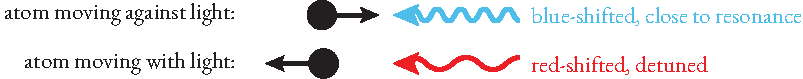
\includegraphics[]{\imagepath/scattering_force_detuning/scattering_force_detuning.pdf}
    \caption{Atoms moving against the direction of laser propagation see the laser light blue-shifted, atoms moving in the other direction see it red-shifted. For negative laser detuning ($\delta_\text{laser} < 0$) the former sense the light as it is close to resonance, the latter do not sense it as it is far detuned for them.}\label{fig:scattering_force_detuning}
\end{figure}

\paragraph*{Doppler limit} While the momentum gained by spontaneous emission of photons averages to zero, the square of momentum $\vec p_\text{after decay}^2$ gained from the spontaneous decays does not. This means that the atom is always left with a finite amount of kinetic energy from the recoil of emitted photons. The magnitude of this leftover energy is related to the decay rate $\Gamma$ and is called the Doppler limit:
\begin{align}
    k_\text{B} T_\text{D} = \frac{\hbar \Gamma}{2}
\end{align}
Laser cooling techniques using spontaneous emission of photons, by principle, cannot provide cooling below this limit (neglecting any coincidental sub-Doppler cooling effects)~\cite{foot_atomic_2005}.
\todo{mention recoil limit}


\subsection*{Magneto-optical Traps}
Magneto-optical traps use light scattering on atoms in order to cool and spatially confine atoms. They have become a standard tool in ultracold neutral atom experiments over the last decades.

\paragraph{Optical molasses} Magneto-optical traps make use of the optical molasses technique for slowing down atoms. As discussed above, light scattering provides a decelerating force opposite the direction of laser beams for red detuning. By using three pairs of counter-propagating laser beams, one pair in each spatial degree of freedom, atoms are decelerated in each direction. For an atom of speed $v$, travelling at an angle $\theta$ with respect to the counter-propagating beams with wave number $k$, the scattering force of two counter-propagating beams adds up to
\begin{align}\label{eq:optical_molasses_force}
    F_\text{OM} = F_\text{scatter}(\delta = \omega_\text{laser} - \omega_\text{transition} - kv \cos \theta) - F_\text{scatter}(\delta = \omega_\text{laser} - \omega_\text{transition} + kv \cos \theta).
\end{align}
For slow velocities $\ll \frac{\Gamma}{k}$, the force can be linearized as a friction force:
\begin{equation}\label{eq:optical_molasses_force_linearized}
    \begin{split}
        F_\text{OM} \approx - 2 \pdv{F_\text{scatter}}{\omega} k v \cos \theta \equiv -( \alpha \cos \theta) v
    \end{split}
\end{equation}
with damping $\alpha = 2k \pdv{F}{\omega} = -8 \hbar k^2 s_0 \frac{\delta/\Gamma}{{\left(1+s_0+{{(2\delta/\Gamma)}}^2\right)}^2}$ where low saturation $s_0 \ll 1$ is assumed~\cite{foot_atomic_2005, metcalf_laser_1999}. The velocity-dependence of the optical molasses deceleration force is depicted in figure~\ref{fig:optical_molasses_force}. Slow atoms don't sense a net force whereas moving atoms are decelerated as they compensate the detuning of the light with the Doppler shift. For detunings $\delta \approx -0.5 \Gamma$, the maximum of the force is approximately at the resonance speed, thus at $v \approx \pm \frac{\delta}{k}$.

\begin{figure}
    \centering
    \begin{pgfpicture}
        \pgftext{%% Creator: Matplotlib, PGF backend
%%
%% To include the figure in your LaTeX document, write
%%   \input{<filename>.pgf}
%%
%% Make sure the required packages are loaded in your preamble
%%   \usepackage{pgf}
%%
%% Also ensure that all the required font packages are loaded; for instance,
%% the lmodern package is sometimes necessary when using math font.
%%   \usepackage{lmodern}
%%
%% Figures using additional raster images can only be included by \input if
%% they are in the same directory as the main LaTeX file. For loading figures
%% from other directories you can use the `import` package
%%   \usepackage{import}
%%
%% and then include the figures with
%%   \import{<path to file>}{<filename>.pgf}
%%
%% Matplotlib used the following preamble
%%   \usepackage{fontspec}
%%   \setmainfont{DejaVuSerif.ttf}[Path=\detokenize{/usr/local/lib/python3.8/dist-packages/matplotlib/mpl-data/fonts/ttf/}]
%%   \setsansfont{DejaVuSans.ttf}[Path=\detokenize{/usr/local/lib/python3.8/dist-packages/matplotlib/mpl-data/fonts/ttf/}]
%%   \setmonofont{DejaVuSansMono.ttf}[Path=\detokenize{/usr/local/lib/python3.8/dist-packages/matplotlib/mpl-data/fonts/ttf/}]
%%
\begingroup%
\makeatletter%
\begin{pgfpicture}%
\pgfpathrectangle{\pgfpointorigin}{\pgfqpoint{3.812959in}{2.627542in}}%
\pgfusepath{use as bounding box, clip}%
\begin{pgfscope}%
\pgfsetbuttcap%
\pgfsetmiterjoin%
\pgfsetlinewidth{0.000000pt}%
\definecolor{currentstroke}{rgb}{1.000000,1.000000,1.000000}%
\pgfsetstrokecolor{currentstroke}%
\pgfsetstrokeopacity{0.000000}%
\pgfsetdash{}{0pt}%
\pgfpathmoveto{\pgfqpoint{0.000000in}{0.000000in}}%
\pgfpathlineto{\pgfqpoint{3.812959in}{0.000000in}}%
\pgfpathlineto{\pgfqpoint{3.812959in}{2.627542in}}%
\pgfpathlineto{\pgfqpoint{0.000000in}{2.627542in}}%
\pgfpathlineto{\pgfqpoint{0.000000in}{0.000000in}}%
\pgfpathclose%
\pgfusepath{}%
\end{pgfscope}%
\begin{pgfscope}%
\pgfsetbuttcap%
\pgfsetmiterjoin%
\definecolor{currentfill}{rgb}{1.000000,1.000000,1.000000}%
\pgfsetfillcolor{currentfill}%
\pgfsetlinewidth{0.000000pt}%
\definecolor{currentstroke}{rgb}{0.000000,0.000000,0.000000}%
\pgfsetstrokecolor{currentstroke}%
\pgfsetstrokeopacity{0.000000}%
\pgfsetdash{}{0pt}%
\pgfpathmoveto{\pgfqpoint{0.756020in}{0.499970in}}%
\pgfpathlineto{\pgfqpoint{3.712959in}{0.499970in}}%
\pgfpathlineto{\pgfqpoint{3.712959in}{2.527542in}}%
\pgfpathlineto{\pgfqpoint{0.756020in}{2.527542in}}%
\pgfpathlineto{\pgfqpoint{0.756020in}{0.499970in}}%
\pgfpathclose%
\pgfusepath{fill}%
\end{pgfscope}%
\begin{pgfscope}%
\pgfpathrectangle{\pgfqpoint{0.756020in}{0.499970in}}{\pgfqpoint{2.956938in}{2.027572in}}%
\pgfusepath{clip}%
\pgfsetrectcap%
\pgfsetroundjoin%
\pgfsetlinewidth{0.803000pt}%
\definecolor{currentstroke}{rgb}{0.690196,0.690196,0.690196}%
\pgfsetstrokecolor{currentstroke}%
\pgfsetdash{}{0pt}%
\pgfpathmoveto{\pgfqpoint{0.890427in}{0.499970in}}%
\pgfpathlineto{\pgfqpoint{0.890427in}{2.527542in}}%
\pgfusepath{stroke}%
\end{pgfscope}%
\begin{pgfscope}%
\pgfsetbuttcap%
\pgfsetroundjoin%
\definecolor{currentfill}{rgb}{0.000000,0.000000,0.000000}%
\pgfsetfillcolor{currentfill}%
\pgfsetlinewidth{0.803000pt}%
\definecolor{currentstroke}{rgb}{0.000000,0.000000,0.000000}%
\pgfsetstrokecolor{currentstroke}%
\pgfsetdash{}{0pt}%
\pgfsys@defobject{currentmarker}{\pgfqpoint{0.000000in}{-0.048611in}}{\pgfqpoint{0.000000in}{0.000000in}}{%
\pgfpathmoveto{\pgfqpoint{0.000000in}{0.000000in}}%
\pgfpathlineto{\pgfqpoint{0.000000in}{-0.048611in}}%
\pgfusepath{stroke,fill}%
}%
\begin{pgfscope}%
\pgfsys@transformshift{0.890427in}{0.499970in}%
\pgfsys@useobject{currentmarker}{}%
\end{pgfscope}%
\end{pgfscope}%
\begin{pgfscope}%
\definecolor{textcolor}{rgb}{0.000000,0.000000,0.000000}%
\pgfsetstrokecolor{textcolor}%
\pgfsetfillcolor{textcolor}%
\pgftext[x=0.890427in,y=0.402748in,,top]{\color{textcolor}\rmfamily\fontsize{9.000000}{10.800000}\selectfont \ensuremath{-}\ensuremath{2}}%
\end{pgfscope}%
\begin{pgfscope}%
\pgfpathrectangle{\pgfqpoint{0.756020in}{0.499970in}}{\pgfqpoint{2.956938in}{2.027572in}}%
\pgfusepath{clip}%
\pgfsetrectcap%
\pgfsetroundjoin%
\pgfsetlinewidth{0.803000pt}%
\definecolor{currentstroke}{rgb}{0.690196,0.690196,0.690196}%
\pgfsetstrokecolor{currentstroke}%
\pgfsetdash{}{0pt}%
\pgfpathmoveto{\pgfqpoint{1.562458in}{0.499970in}}%
\pgfpathlineto{\pgfqpoint{1.562458in}{2.527542in}}%
\pgfusepath{stroke}%
\end{pgfscope}%
\begin{pgfscope}%
\pgfsetbuttcap%
\pgfsetroundjoin%
\definecolor{currentfill}{rgb}{0.000000,0.000000,0.000000}%
\pgfsetfillcolor{currentfill}%
\pgfsetlinewidth{0.803000pt}%
\definecolor{currentstroke}{rgb}{0.000000,0.000000,0.000000}%
\pgfsetstrokecolor{currentstroke}%
\pgfsetdash{}{0pt}%
\pgfsys@defobject{currentmarker}{\pgfqpoint{0.000000in}{-0.048611in}}{\pgfqpoint{0.000000in}{0.000000in}}{%
\pgfpathmoveto{\pgfqpoint{0.000000in}{0.000000in}}%
\pgfpathlineto{\pgfqpoint{0.000000in}{-0.048611in}}%
\pgfusepath{stroke,fill}%
}%
\begin{pgfscope}%
\pgfsys@transformshift{1.562458in}{0.499970in}%
\pgfsys@useobject{currentmarker}{}%
\end{pgfscope}%
\end{pgfscope}%
\begin{pgfscope}%
\definecolor{textcolor}{rgb}{0.000000,0.000000,0.000000}%
\pgfsetstrokecolor{textcolor}%
\pgfsetfillcolor{textcolor}%
\pgftext[x=1.562458in,y=0.402748in,,top]{\color{textcolor}\rmfamily\fontsize{9.000000}{10.800000}\selectfont \ensuremath{-}\ensuremath{1}}%
\end{pgfscope}%
\begin{pgfscope}%
\pgfpathrectangle{\pgfqpoint{0.756020in}{0.499970in}}{\pgfqpoint{2.956938in}{2.027572in}}%
\pgfusepath{clip}%
\pgfsetrectcap%
\pgfsetroundjoin%
\pgfsetlinewidth{0.803000pt}%
\definecolor{currentstroke}{rgb}{0.690196,0.690196,0.690196}%
\pgfsetstrokecolor{currentstroke}%
\pgfsetdash{}{0pt}%
\pgfpathmoveto{\pgfqpoint{2.234489in}{0.499970in}}%
\pgfpathlineto{\pgfqpoint{2.234489in}{2.527542in}}%
\pgfusepath{stroke}%
\end{pgfscope}%
\begin{pgfscope}%
\pgfsetbuttcap%
\pgfsetroundjoin%
\definecolor{currentfill}{rgb}{0.000000,0.000000,0.000000}%
\pgfsetfillcolor{currentfill}%
\pgfsetlinewidth{0.803000pt}%
\definecolor{currentstroke}{rgb}{0.000000,0.000000,0.000000}%
\pgfsetstrokecolor{currentstroke}%
\pgfsetdash{}{0pt}%
\pgfsys@defobject{currentmarker}{\pgfqpoint{0.000000in}{-0.048611in}}{\pgfqpoint{0.000000in}{0.000000in}}{%
\pgfpathmoveto{\pgfqpoint{0.000000in}{0.000000in}}%
\pgfpathlineto{\pgfqpoint{0.000000in}{-0.048611in}}%
\pgfusepath{stroke,fill}%
}%
\begin{pgfscope}%
\pgfsys@transformshift{2.234489in}{0.499970in}%
\pgfsys@useobject{currentmarker}{}%
\end{pgfscope}%
\end{pgfscope}%
\begin{pgfscope}%
\definecolor{textcolor}{rgb}{0.000000,0.000000,0.000000}%
\pgfsetstrokecolor{textcolor}%
\pgfsetfillcolor{textcolor}%
\pgftext[x=2.234489in,y=0.402748in,,top]{\color{textcolor}\rmfamily\fontsize{9.000000}{10.800000}\selectfont \ensuremath{0}}%
\end{pgfscope}%
\begin{pgfscope}%
\pgfpathrectangle{\pgfqpoint{0.756020in}{0.499970in}}{\pgfqpoint{2.956938in}{2.027572in}}%
\pgfusepath{clip}%
\pgfsetrectcap%
\pgfsetroundjoin%
\pgfsetlinewidth{0.803000pt}%
\definecolor{currentstroke}{rgb}{0.690196,0.690196,0.690196}%
\pgfsetstrokecolor{currentstroke}%
\pgfsetdash{}{0pt}%
\pgfpathmoveto{\pgfqpoint{2.906521in}{0.499970in}}%
\pgfpathlineto{\pgfqpoint{2.906521in}{2.527542in}}%
\pgfusepath{stroke}%
\end{pgfscope}%
\begin{pgfscope}%
\pgfsetbuttcap%
\pgfsetroundjoin%
\definecolor{currentfill}{rgb}{0.000000,0.000000,0.000000}%
\pgfsetfillcolor{currentfill}%
\pgfsetlinewidth{0.803000pt}%
\definecolor{currentstroke}{rgb}{0.000000,0.000000,0.000000}%
\pgfsetstrokecolor{currentstroke}%
\pgfsetdash{}{0pt}%
\pgfsys@defobject{currentmarker}{\pgfqpoint{0.000000in}{-0.048611in}}{\pgfqpoint{0.000000in}{0.000000in}}{%
\pgfpathmoveto{\pgfqpoint{0.000000in}{0.000000in}}%
\pgfpathlineto{\pgfqpoint{0.000000in}{-0.048611in}}%
\pgfusepath{stroke,fill}%
}%
\begin{pgfscope}%
\pgfsys@transformshift{2.906521in}{0.499970in}%
\pgfsys@useobject{currentmarker}{}%
\end{pgfscope}%
\end{pgfscope}%
\begin{pgfscope}%
\definecolor{textcolor}{rgb}{0.000000,0.000000,0.000000}%
\pgfsetstrokecolor{textcolor}%
\pgfsetfillcolor{textcolor}%
\pgftext[x=2.906521in,y=0.402748in,,top]{\color{textcolor}\rmfamily\fontsize{9.000000}{10.800000}\selectfont \ensuremath{1}}%
\end{pgfscope}%
\begin{pgfscope}%
\pgfpathrectangle{\pgfqpoint{0.756020in}{0.499970in}}{\pgfqpoint{2.956938in}{2.027572in}}%
\pgfusepath{clip}%
\pgfsetrectcap%
\pgfsetroundjoin%
\pgfsetlinewidth{0.803000pt}%
\definecolor{currentstroke}{rgb}{0.690196,0.690196,0.690196}%
\pgfsetstrokecolor{currentstroke}%
\pgfsetdash{}{0pt}%
\pgfpathmoveto{\pgfqpoint{3.578552in}{0.499970in}}%
\pgfpathlineto{\pgfqpoint{3.578552in}{2.527542in}}%
\pgfusepath{stroke}%
\end{pgfscope}%
\begin{pgfscope}%
\pgfsetbuttcap%
\pgfsetroundjoin%
\definecolor{currentfill}{rgb}{0.000000,0.000000,0.000000}%
\pgfsetfillcolor{currentfill}%
\pgfsetlinewidth{0.803000pt}%
\definecolor{currentstroke}{rgb}{0.000000,0.000000,0.000000}%
\pgfsetstrokecolor{currentstroke}%
\pgfsetdash{}{0pt}%
\pgfsys@defobject{currentmarker}{\pgfqpoint{0.000000in}{-0.048611in}}{\pgfqpoint{0.000000in}{0.000000in}}{%
\pgfpathmoveto{\pgfqpoint{0.000000in}{0.000000in}}%
\pgfpathlineto{\pgfqpoint{0.000000in}{-0.048611in}}%
\pgfusepath{stroke,fill}%
}%
\begin{pgfscope}%
\pgfsys@transformshift{3.578552in}{0.499970in}%
\pgfsys@useobject{currentmarker}{}%
\end{pgfscope}%
\end{pgfscope}%
\begin{pgfscope}%
\definecolor{textcolor}{rgb}{0.000000,0.000000,0.000000}%
\pgfsetstrokecolor{textcolor}%
\pgfsetfillcolor{textcolor}%
\pgftext[x=3.578552in,y=0.402748in,,top]{\color{textcolor}\rmfamily\fontsize{9.000000}{10.800000}\selectfont \ensuremath{2}}%
\end{pgfscope}%
\begin{pgfscope}%
\definecolor{textcolor}{rgb}{0.000000,0.000000,0.000000}%
\pgfsetstrokecolor{textcolor}%
\pgfsetfillcolor{textcolor}%
\pgftext[x=2.234489in,y=0.226221in,,top]{\color{textcolor}\rmfamily\fontsize{9.000000}{10.800000}\selectfont speed in \(\displaystyle \Gamma/k\)}%
\end{pgfscope}%
\begin{pgfscope}%
\pgfpathrectangle{\pgfqpoint{0.756020in}{0.499970in}}{\pgfqpoint{2.956938in}{2.027572in}}%
\pgfusepath{clip}%
\pgfsetrectcap%
\pgfsetroundjoin%
\pgfsetlinewidth{0.803000pt}%
\definecolor{currentstroke}{rgb}{0.690196,0.690196,0.690196}%
\pgfsetstrokecolor{currentstroke}%
\pgfsetdash{}{0pt}%
\pgfpathmoveto{\pgfqpoint{0.756020in}{0.677950in}}%
\pgfpathlineto{\pgfqpoint{3.712959in}{0.677950in}}%
\pgfusepath{stroke}%
\end{pgfscope}%
\begin{pgfscope}%
\pgfsetbuttcap%
\pgfsetroundjoin%
\definecolor{currentfill}{rgb}{0.000000,0.000000,0.000000}%
\pgfsetfillcolor{currentfill}%
\pgfsetlinewidth{0.803000pt}%
\definecolor{currentstroke}{rgb}{0.000000,0.000000,0.000000}%
\pgfsetstrokecolor{currentstroke}%
\pgfsetdash{}{0pt}%
\pgfsys@defobject{currentmarker}{\pgfqpoint{-0.048611in}{0.000000in}}{\pgfqpoint{-0.000000in}{0.000000in}}{%
\pgfpathmoveto{\pgfqpoint{-0.000000in}{0.000000in}}%
\pgfpathlineto{\pgfqpoint{-0.048611in}{0.000000in}}%
\pgfusepath{stroke,fill}%
}%
\begin{pgfscope}%
\pgfsys@transformshift{0.756020in}{0.677950in}%
\pgfsys@useobject{currentmarker}{}%
\end{pgfscope}%
\end{pgfscope}%
\begin{pgfscope}%
\definecolor{textcolor}{rgb}{0.000000,0.000000,0.000000}%
\pgfsetstrokecolor{textcolor}%
\pgfsetfillcolor{textcolor}%
\pgftext[x=0.280556in, y=0.630464in, left, base]{\color{textcolor}\rmfamily\fontsize{9.000000}{10.800000}\selectfont \ensuremath{-}\ensuremath{0.04}}%
\end{pgfscope}%
\begin{pgfscope}%
\pgfpathrectangle{\pgfqpoint{0.756020in}{0.499970in}}{\pgfqpoint{2.956938in}{2.027572in}}%
\pgfusepath{clip}%
\pgfsetrectcap%
\pgfsetroundjoin%
\pgfsetlinewidth{0.803000pt}%
\definecolor{currentstroke}{rgb}{0.690196,0.690196,0.690196}%
\pgfsetstrokecolor{currentstroke}%
\pgfsetdash{}{0pt}%
\pgfpathmoveto{\pgfqpoint{0.756020in}{1.095853in}}%
\pgfpathlineto{\pgfqpoint{3.712959in}{1.095853in}}%
\pgfusepath{stroke}%
\end{pgfscope}%
\begin{pgfscope}%
\pgfsetbuttcap%
\pgfsetroundjoin%
\definecolor{currentfill}{rgb}{0.000000,0.000000,0.000000}%
\pgfsetfillcolor{currentfill}%
\pgfsetlinewidth{0.803000pt}%
\definecolor{currentstroke}{rgb}{0.000000,0.000000,0.000000}%
\pgfsetstrokecolor{currentstroke}%
\pgfsetdash{}{0pt}%
\pgfsys@defobject{currentmarker}{\pgfqpoint{-0.048611in}{0.000000in}}{\pgfqpoint{-0.000000in}{0.000000in}}{%
\pgfpathmoveto{\pgfqpoint{-0.000000in}{0.000000in}}%
\pgfpathlineto{\pgfqpoint{-0.048611in}{0.000000in}}%
\pgfusepath{stroke,fill}%
}%
\begin{pgfscope}%
\pgfsys@transformshift{0.756020in}{1.095853in}%
\pgfsys@useobject{currentmarker}{}%
\end{pgfscope}%
\end{pgfscope}%
\begin{pgfscope}%
\definecolor{textcolor}{rgb}{0.000000,0.000000,0.000000}%
\pgfsetstrokecolor{textcolor}%
\pgfsetfillcolor{textcolor}%
\pgftext[x=0.280556in, y=1.048368in, left, base]{\color{textcolor}\rmfamily\fontsize{9.000000}{10.800000}\selectfont \ensuremath{-}\ensuremath{0.02}}%
\end{pgfscope}%
\begin{pgfscope}%
\pgfpathrectangle{\pgfqpoint{0.756020in}{0.499970in}}{\pgfqpoint{2.956938in}{2.027572in}}%
\pgfusepath{clip}%
\pgfsetrectcap%
\pgfsetroundjoin%
\pgfsetlinewidth{0.803000pt}%
\definecolor{currentstroke}{rgb}{0.690196,0.690196,0.690196}%
\pgfsetstrokecolor{currentstroke}%
\pgfsetdash{}{0pt}%
\pgfpathmoveto{\pgfqpoint{0.756020in}{1.513756in}}%
\pgfpathlineto{\pgfqpoint{3.712959in}{1.513756in}}%
\pgfusepath{stroke}%
\end{pgfscope}%
\begin{pgfscope}%
\pgfsetbuttcap%
\pgfsetroundjoin%
\definecolor{currentfill}{rgb}{0.000000,0.000000,0.000000}%
\pgfsetfillcolor{currentfill}%
\pgfsetlinewidth{0.803000pt}%
\definecolor{currentstroke}{rgb}{0.000000,0.000000,0.000000}%
\pgfsetstrokecolor{currentstroke}%
\pgfsetdash{}{0pt}%
\pgfsys@defobject{currentmarker}{\pgfqpoint{-0.048611in}{0.000000in}}{\pgfqpoint{-0.000000in}{0.000000in}}{%
\pgfpathmoveto{\pgfqpoint{-0.000000in}{0.000000in}}%
\pgfpathlineto{\pgfqpoint{-0.048611in}{0.000000in}}%
\pgfusepath{stroke,fill}%
}%
\begin{pgfscope}%
\pgfsys@transformshift{0.756020in}{1.513756in}%
\pgfsys@useobject{currentmarker}{}%
\end{pgfscope}%
\end{pgfscope}%
\begin{pgfscope}%
\definecolor{textcolor}{rgb}{0.000000,0.000000,0.000000}%
\pgfsetstrokecolor{textcolor}%
\pgfsetfillcolor{textcolor}%
\pgftext[x=0.380478in, y=1.466271in, left, base]{\color{textcolor}\rmfamily\fontsize{9.000000}{10.800000}\selectfont \ensuremath{0.00}}%
\end{pgfscope}%
\begin{pgfscope}%
\pgfpathrectangle{\pgfqpoint{0.756020in}{0.499970in}}{\pgfqpoint{2.956938in}{2.027572in}}%
\pgfusepath{clip}%
\pgfsetrectcap%
\pgfsetroundjoin%
\pgfsetlinewidth{0.803000pt}%
\definecolor{currentstroke}{rgb}{0.690196,0.690196,0.690196}%
\pgfsetstrokecolor{currentstroke}%
\pgfsetdash{}{0pt}%
\pgfpathmoveto{\pgfqpoint{0.756020in}{1.931659in}}%
\pgfpathlineto{\pgfqpoint{3.712959in}{1.931659in}}%
\pgfusepath{stroke}%
\end{pgfscope}%
\begin{pgfscope}%
\pgfsetbuttcap%
\pgfsetroundjoin%
\definecolor{currentfill}{rgb}{0.000000,0.000000,0.000000}%
\pgfsetfillcolor{currentfill}%
\pgfsetlinewidth{0.803000pt}%
\definecolor{currentstroke}{rgb}{0.000000,0.000000,0.000000}%
\pgfsetstrokecolor{currentstroke}%
\pgfsetdash{}{0pt}%
\pgfsys@defobject{currentmarker}{\pgfqpoint{-0.048611in}{0.000000in}}{\pgfqpoint{-0.000000in}{0.000000in}}{%
\pgfpathmoveto{\pgfqpoint{-0.000000in}{0.000000in}}%
\pgfpathlineto{\pgfqpoint{-0.048611in}{0.000000in}}%
\pgfusepath{stroke,fill}%
}%
\begin{pgfscope}%
\pgfsys@transformshift{0.756020in}{1.931659in}%
\pgfsys@useobject{currentmarker}{}%
\end{pgfscope}%
\end{pgfscope}%
\begin{pgfscope}%
\definecolor{textcolor}{rgb}{0.000000,0.000000,0.000000}%
\pgfsetstrokecolor{textcolor}%
\pgfsetfillcolor{textcolor}%
\pgftext[x=0.380478in, y=1.884174in, left, base]{\color{textcolor}\rmfamily\fontsize{9.000000}{10.800000}\selectfont \ensuremath{0.02}}%
\end{pgfscope}%
\begin{pgfscope}%
\pgfpathrectangle{\pgfqpoint{0.756020in}{0.499970in}}{\pgfqpoint{2.956938in}{2.027572in}}%
\pgfusepath{clip}%
\pgfsetrectcap%
\pgfsetroundjoin%
\pgfsetlinewidth{0.803000pt}%
\definecolor{currentstroke}{rgb}{0.690196,0.690196,0.690196}%
\pgfsetstrokecolor{currentstroke}%
\pgfsetdash{}{0pt}%
\pgfpathmoveto{\pgfqpoint{0.756020in}{2.349563in}}%
\pgfpathlineto{\pgfqpoint{3.712959in}{2.349563in}}%
\pgfusepath{stroke}%
\end{pgfscope}%
\begin{pgfscope}%
\pgfsetbuttcap%
\pgfsetroundjoin%
\definecolor{currentfill}{rgb}{0.000000,0.000000,0.000000}%
\pgfsetfillcolor{currentfill}%
\pgfsetlinewidth{0.803000pt}%
\definecolor{currentstroke}{rgb}{0.000000,0.000000,0.000000}%
\pgfsetstrokecolor{currentstroke}%
\pgfsetdash{}{0pt}%
\pgfsys@defobject{currentmarker}{\pgfqpoint{-0.048611in}{0.000000in}}{\pgfqpoint{-0.000000in}{0.000000in}}{%
\pgfpathmoveto{\pgfqpoint{-0.000000in}{0.000000in}}%
\pgfpathlineto{\pgfqpoint{-0.048611in}{0.000000in}}%
\pgfusepath{stroke,fill}%
}%
\begin{pgfscope}%
\pgfsys@transformshift{0.756020in}{2.349563in}%
\pgfsys@useobject{currentmarker}{}%
\end{pgfscope}%
\end{pgfscope}%
\begin{pgfscope}%
\definecolor{textcolor}{rgb}{0.000000,0.000000,0.000000}%
\pgfsetstrokecolor{textcolor}%
\pgfsetfillcolor{textcolor}%
\pgftext[x=0.380478in, y=2.302077in, left, base]{\color{textcolor}\rmfamily\fontsize{9.000000}{10.800000}\selectfont \ensuremath{0.04}}%
\end{pgfscope}%
\begin{pgfscope}%
\definecolor{textcolor}{rgb}{0.000000,0.000000,0.000000}%
\pgfsetstrokecolor{textcolor}%
\pgfsetfillcolor{textcolor}%
\pgftext[x=0.225000in,y=1.513756in,,bottom,rotate=90.000000]{\color{textcolor}\rmfamily\fontsize{9.000000}{10.800000}\selectfont \(\displaystyle F_\mathrm{OM}\) in \(\displaystyle 1/(\hbar k \Gamma)\)}%
\end{pgfscope}%
\begin{pgfscope}%
\pgfpathrectangle{\pgfqpoint{0.756020in}{0.499970in}}{\pgfqpoint{2.956938in}{2.027572in}}%
\pgfusepath{clip}%
\pgfsetrectcap%
\pgfsetroundjoin%
\pgfsetlinewidth{1.505625pt}%
\definecolor{currentstroke}{rgb}{1.000000,0.000000,0.000000}%
\pgfsetstrokecolor{currentstroke}%
\pgfsetstrokeopacity{0.840000}%
\pgfsetdash{}{0pt}%
\pgfpathmoveto{\pgfqpoint{0.890427in}{1.577168in}}%
\pgfpathlineto{\pgfqpoint{0.971340in}{1.589672in}}%
\pgfpathlineto{\pgfqpoint{1.043263in}{1.603611in}}%
\pgfpathlineto{\pgfqpoint{1.106196in}{1.618637in}}%
\pgfpathlineto{\pgfqpoint{1.169129in}{1.637042in}}%
\pgfpathlineto{\pgfqpoint{1.223071in}{1.656196in}}%
\pgfpathlineto{\pgfqpoint{1.268023in}{1.675088in}}%
\pgfpathlineto{\pgfqpoint{1.312975in}{1.697183in}}%
\pgfpathlineto{\pgfqpoint{1.357927in}{1.723072in}}%
\pgfpathlineto{\pgfqpoint{1.393888in}{1.746967in}}%
\pgfpathlineto{\pgfqpoint{1.429850in}{1.774095in}}%
\pgfpathlineto{\pgfqpoint{1.465811in}{1.804837in}}%
\pgfpathlineto{\pgfqpoint{1.501773in}{1.839548in}}%
\pgfpathlineto{\pgfqpoint{1.537734in}{1.878505in}}%
\pgfpathlineto{\pgfqpoint{1.573696in}{1.921819in}}%
\pgfpathlineto{\pgfqpoint{1.618648in}{1.981777in}}%
\pgfpathlineto{\pgfqpoint{1.672590in}{2.060187in}}%
\pgfpathlineto{\pgfqpoint{1.744513in}{2.165048in}}%
\pgfpathlineto{\pgfqpoint{1.771485in}{2.199710in}}%
\pgfpathlineto{\pgfqpoint{1.798456in}{2.228963in}}%
\pgfpathlineto{\pgfqpoint{1.816436in}{2.244453in}}%
\pgfpathlineto{\pgfqpoint{1.834417in}{2.256050in}}%
\pgfpathlineto{\pgfqpoint{1.852398in}{2.263225in}}%
\pgfpathlineto{\pgfqpoint{1.870379in}{2.265538in}}%
\pgfpathlineto{\pgfqpoint{1.888360in}{2.262659in}}%
\pgfpathlineto{\pgfqpoint{1.906340in}{2.254400in}}%
\pgfpathlineto{\pgfqpoint{1.924321in}{2.240716in}}%
\pgfpathlineto{\pgfqpoint{1.942302in}{2.221715in}}%
\pgfpathlineto{\pgfqpoint{1.960283in}{2.197642in}}%
\pgfpathlineto{\pgfqpoint{1.978263in}{2.168860in}}%
\pgfpathlineto{\pgfqpoint{2.005235in}{2.117861in}}%
\pgfpathlineto{\pgfqpoint{2.032206in}{2.059032in}}%
\pgfpathlineto{\pgfqpoint{2.068167in}{1.971498in}}%
\pgfpathlineto{\pgfqpoint{2.113119in}{1.852728in}}%
\pgfpathlineto{\pgfqpoint{2.194033in}{1.627771in}}%
\pgfpathlineto{\pgfqpoint{2.364850in}{1.150461in}}%
\pgfpathlineto{\pgfqpoint{2.409802in}{1.033345in}}%
\pgfpathlineto{\pgfqpoint{2.445764in}{0.948113in}}%
\pgfpathlineto{\pgfqpoint{2.472735in}{0.891693in}}%
\pgfpathlineto{\pgfqpoint{2.499706in}{0.843699in}}%
\pgfpathlineto{\pgfqpoint{2.517687in}{0.817220in}}%
\pgfpathlineto{\pgfqpoint{2.535667in}{0.795644in}}%
\pgfpathlineto{\pgfqpoint{2.553648in}{0.779280in}}%
\pgfpathlineto{\pgfqpoint{2.571629in}{0.768304in}}%
\pgfpathlineto{\pgfqpoint{2.589610in}{0.762749in}}%
\pgfpathlineto{\pgfqpoint{2.607591in}{0.762499in}}%
\pgfpathlineto{\pgfqpoint{2.625571in}{0.767292in}}%
\pgfpathlineto{\pgfqpoint{2.643552in}{0.776740in}}%
\pgfpathlineto{\pgfqpoint{2.661533in}{0.790353in}}%
\pgfpathlineto{\pgfqpoint{2.679514in}{0.807573in}}%
\pgfpathlineto{\pgfqpoint{2.706485in}{0.838854in}}%
\pgfpathlineto{\pgfqpoint{2.742446in}{0.887609in}}%
\pgfpathlineto{\pgfqpoint{2.814369in}{0.993991in}}%
\pgfpathlineto{\pgfqpoint{2.868312in}{1.070440in}}%
\pgfpathlineto{\pgfqpoint{2.913264in}{1.127893in}}%
\pgfpathlineto{\pgfqpoint{2.949225in}{1.169029in}}%
\pgfpathlineto{\pgfqpoint{2.985187in}{1.205836in}}%
\pgfpathlineto{\pgfqpoint{3.021148in}{1.238521in}}%
\pgfpathlineto{\pgfqpoint{3.057110in}{1.267409in}}%
\pgfpathlineto{\pgfqpoint{3.093071in}{1.292873in}}%
\pgfpathlineto{\pgfqpoint{3.138023in}{1.320465in}}%
\pgfpathlineto{\pgfqpoint{3.182975in}{1.344002in}}%
\pgfpathlineto{\pgfqpoint{3.227927in}{1.364109in}}%
\pgfpathlineto{\pgfqpoint{3.281870in}{1.384469in}}%
\pgfpathlineto{\pgfqpoint{3.335812in}{1.401449in}}%
\pgfpathlineto{\pgfqpoint{3.398745in}{1.417826in}}%
\pgfpathlineto{\pgfqpoint{3.470668in}{1.432966in}}%
\pgfpathlineto{\pgfqpoint{3.551581in}{1.446497in}}%
\pgfpathlineto{\pgfqpoint{3.578552in}{1.450344in}}%
\pgfpathlineto{\pgfqpoint{3.578552in}{1.450344in}}%
\pgfusepath{stroke}%
\end{pgfscope}%
\begin{pgfscope}%
\pgfpathrectangle{\pgfqpoint{0.756020in}{0.499970in}}{\pgfqpoint{2.956938in}{2.027572in}}%
\pgfusepath{clip}%
\pgfsetrectcap%
\pgfsetroundjoin%
\pgfsetlinewidth{1.505625pt}%
\definecolor{currentstroke}{rgb}{1.000000,0.000000,0.000000}%
\pgfsetstrokecolor{currentstroke}%
\pgfsetstrokeopacity{0.480000}%
\pgfsetdash{}{0pt}%
\pgfpathmoveto{\pgfqpoint{0.890427in}{1.690450in}}%
\pgfpathlineto{\pgfqpoint{0.935379in}{1.712311in}}%
\pgfpathlineto{\pgfqpoint{0.980330in}{1.737727in}}%
\pgfpathlineto{\pgfqpoint{1.025282in}{1.767342in}}%
\pgfpathlineto{\pgfqpoint{1.061244in}{1.794547in}}%
\pgfpathlineto{\pgfqpoint{1.097205in}{1.825312in}}%
\pgfpathlineto{\pgfqpoint{1.133167in}{1.860053in}}%
\pgfpathlineto{\pgfqpoint{1.169129in}{1.899161in}}%
\pgfpathlineto{\pgfqpoint{1.205090in}{1.942949in}}%
\pgfpathlineto{\pgfqpoint{1.241052in}{1.991559in}}%
\pgfpathlineto{\pgfqpoint{1.277013in}{2.044840in}}%
\pgfpathlineto{\pgfqpoint{1.321965in}{2.117001in}}%
\pgfpathlineto{\pgfqpoint{1.429850in}{2.294556in}}%
\pgfpathlineto{\pgfqpoint{1.456821in}{2.332237in}}%
\pgfpathlineto{\pgfqpoint{1.483792in}{2.363551in}}%
\pgfpathlineto{\pgfqpoint{1.501773in}{2.379946in}}%
\pgfpathlineto{\pgfqpoint{1.519754in}{2.392175in}}%
\pgfpathlineto{\pgfqpoint{1.537734in}{2.399839in}}%
\pgfpathlineto{\pgfqpoint{1.555715in}{2.402661in}}%
\pgfpathlineto{\pgfqpoint{1.573696in}{2.400507in}}%
\pgfpathlineto{\pgfqpoint{1.591677in}{2.393393in}}%
\pgfpathlineto{\pgfqpoint{1.609658in}{2.381486in}}%
\pgfpathlineto{\pgfqpoint{1.627638in}{2.365088in}}%
\pgfpathlineto{\pgfqpoint{1.645619in}{2.344620in}}%
\pgfpathlineto{\pgfqpoint{1.672590in}{2.307402in}}%
\pgfpathlineto{\pgfqpoint{1.699561in}{2.264069in}}%
\pgfpathlineto{\pgfqpoint{1.735523in}{2.200111in}}%
\pgfpathlineto{\pgfqpoint{1.861388in}{1.969149in}}%
\pgfpathlineto{\pgfqpoint{1.906340in}{1.895390in}}%
\pgfpathlineto{\pgfqpoint{1.951292in}{1.828307in}}%
\pgfpathlineto{\pgfqpoint{1.996244in}{1.767585in}}%
\pgfpathlineto{\pgfqpoint{2.041196in}{1.712431in}}%
\pgfpathlineto{\pgfqpoint{2.086148in}{1.661838in}}%
\pgfpathlineto{\pgfqpoint{2.140090in}{1.605627in}}%
\pgfpathlineto{\pgfqpoint{2.221004in}{1.526657in}}%
\pgfpathlineto{\pgfqpoint{2.337879in}{1.412785in}}%
\pgfpathlineto{\pgfqpoint{2.391821in}{1.355869in}}%
\pgfpathlineto{\pgfqpoint{2.436773in}{1.304449in}}%
\pgfpathlineto{\pgfqpoint{2.481725in}{1.248258in}}%
\pgfpathlineto{\pgfqpoint{2.526677in}{1.186317in}}%
\pgfpathlineto{\pgfqpoint{2.571629in}{1.117901in}}%
\pgfpathlineto{\pgfqpoint{2.616581in}{1.042840in}}%
\pgfpathlineto{\pgfqpoint{2.670523in}{0.945278in}}%
\pgfpathlineto{\pgfqpoint{2.769418in}{0.763443in}}%
\pgfpathlineto{\pgfqpoint{2.796389in}{0.720110in}}%
\pgfpathlineto{\pgfqpoint{2.823360in}{0.682892in}}%
\pgfpathlineto{\pgfqpoint{2.841341in}{0.662424in}}%
\pgfpathlineto{\pgfqpoint{2.859321in}{0.646026in}}%
\pgfpathlineto{\pgfqpoint{2.877302in}{0.634119in}}%
\pgfpathlineto{\pgfqpoint{2.895283in}{0.627005in}}%
\pgfpathlineto{\pgfqpoint{2.913264in}{0.624851in}}%
\pgfpathlineto{\pgfqpoint{2.931245in}{0.627673in}}%
\pgfpathlineto{\pgfqpoint{2.949225in}{0.635337in}}%
\pgfpathlineto{\pgfqpoint{2.967206in}{0.647566in}}%
\pgfpathlineto{\pgfqpoint{2.985187in}{0.663961in}}%
\pgfpathlineto{\pgfqpoint{3.003168in}{0.684032in}}%
\pgfpathlineto{\pgfqpoint{3.030139in}{0.719810in}}%
\pgfpathlineto{\pgfqpoint{3.066100in}{0.775040in}}%
\pgfpathlineto{\pgfqpoint{3.129033in}{0.880439in}}%
\pgfpathlineto{\pgfqpoint{3.182975in}{0.968681in}}%
\pgfpathlineto{\pgfqpoint{3.227927in}{1.035953in}}%
\pgfpathlineto{\pgfqpoint{3.263889in}{1.084563in}}%
\pgfpathlineto{\pgfqpoint{3.299850in}{1.128351in}}%
\pgfpathlineto{\pgfqpoint{3.335812in}{1.167459in}}%
\pgfpathlineto{\pgfqpoint{3.371774in}{1.202200in}}%
\pgfpathlineto{\pgfqpoint{3.407735in}{1.232965in}}%
\pgfpathlineto{\pgfqpoint{3.443697in}{1.260170in}}%
\pgfpathlineto{\pgfqpoint{3.488649in}{1.289785in}}%
\pgfpathlineto{\pgfqpoint{3.533600in}{1.315201in}}%
\pgfpathlineto{\pgfqpoint{3.578552in}{1.337062in}}%
\pgfpathlineto{\pgfqpoint{3.578552in}{1.337062in}}%
\pgfusepath{stroke}%
\end{pgfscope}%
\begin{pgfscope}%
\pgfpathrectangle{\pgfqpoint{0.756020in}{0.499970in}}{\pgfqpoint{2.956938in}{2.027572in}}%
\pgfusepath{clip}%
\pgfsetrectcap%
\pgfsetroundjoin%
\pgfsetlinewidth{1.505625pt}%
\definecolor{currentstroke}{rgb}{1.000000,0.000000,0.000000}%
\pgfsetstrokecolor{currentstroke}%
\pgfsetstrokeopacity{0.120000}%
\pgfsetdash{}{0pt}%
\pgfpathmoveto{\pgfqpoint{0.890427in}{1.990406in}}%
\pgfpathlineto{\pgfqpoint{0.926388in}{2.042889in}}%
\pgfpathlineto{\pgfqpoint{0.971340in}{2.114648in}}%
\pgfpathlineto{\pgfqpoint{1.043263in}{2.237736in}}%
\pgfpathlineto{\pgfqpoint{1.088215in}{2.312148in}}%
\pgfpathlineto{\pgfqpoint{1.115186in}{2.352088in}}%
\pgfpathlineto{\pgfqpoint{1.142157in}{2.386143in}}%
\pgfpathlineto{\pgfqpoint{1.160138in}{2.404621in}}%
\pgfpathlineto{\pgfqpoint{1.178119in}{2.419113in}}%
\pgfpathlineto{\pgfqpoint{1.196100in}{2.429192in}}%
\pgfpathlineto{\pgfqpoint{1.214081in}{2.434541in}}%
\pgfpathlineto{\pgfqpoint{1.232061in}{2.434981in}}%
\pgfpathlineto{\pgfqpoint{1.250042in}{2.430485in}}%
\pgfpathlineto{\pgfqpoint{1.268023in}{2.421174in}}%
\pgfpathlineto{\pgfqpoint{1.286004in}{2.407314in}}%
\pgfpathlineto{\pgfqpoint{1.303984in}{2.389293in}}%
\pgfpathlineto{\pgfqpoint{1.321965in}{2.367595in}}%
\pgfpathlineto{\pgfqpoint{1.348936in}{2.329362in}}%
\pgfpathlineto{\pgfqpoint{1.384898in}{2.270819in}}%
\pgfpathlineto{\pgfqpoint{1.447831in}{2.159517in}}%
\pgfpathlineto{\pgfqpoint{1.501773in}{2.066149in}}%
\pgfpathlineto{\pgfqpoint{1.546725in}{1.994592in}}%
\pgfpathlineto{\pgfqpoint{1.582686in}{1.942548in}}%
\pgfpathlineto{\pgfqpoint{1.618648in}{1.895318in}}%
\pgfpathlineto{\pgfqpoint{1.654610in}{1.852750in}}%
\pgfpathlineto{\pgfqpoint{1.690571in}{1.814520in}}%
\pgfpathlineto{\pgfqpoint{1.726533in}{1.780221in}}%
\pgfpathlineto{\pgfqpoint{1.771485in}{1.742216in}}%
\pgfpathlineto{\pgfqpoint{1.816436in}{1.708855in}}%
\pgfpathlineto{\pgfqpoint{1.861388in}{1.679381in}}%
\pgfpathlineto{\pgfqpoint{1.915331in}{1.648206in}}%
\pgfpathlineto{\pgfqpoint{1.969273in}{1.620671in}}%
\pgfpathlineto{\pgfqpoint{2.032206in}{1.592036in}}%
\pgfpathlineto{\pgfqpoint{2.113119in}{1.559056in}}%
\pgfpathlineto{\pgfqpoint{2.229994in}{1.515400in}}%
\pgfpathlineto{\pgfqpoint{2.373840in}{1.461408in}}%
\pgfpathlineto{\pgfqpoint{2.454754in}{1.427615in}}%
\pgfpathlineto{\pgfqpoint{2.517687in}{1.398013in}}%
\pgfpathlineto{\pgfqpoint{2.571629in}{1.369365in}}%
\pgfpathlineto{\pgfqpoint{2.616581in}{1.342514in}}%
\pgfpathlineto{\pgfqpoint{2.661533in}{1.312319in}}%
\pgfpathlineto{\pgfqpoint{2.706485in}{1.278092in}}%
\pgfpathlineto{\pgfqpoint{2.742446in}{1.247291in}}%
\pgfpathlineto{\pgfqpoint{2.778408in}{1.212992in}}%
\pgfpathlineto{\pgfqpoint{2.814369in}{1.174762in}}%
\pgfpathlineto{\pgfqpoint{2.850331in}{1.132194in}}%
\pgfpathlineto{\pgfqpoint{2.886293in}{1.084964in}}%
\pgfpathlineto{\pgfqpoint{2.922254in}{1.032920in}}%
\pgfpathlineto{\pgfqpoint{2.967206in}{0.961363in}}%
\pgfpathlineto{\pgfqpoint{3.021148in}{0.867996in}}%
\pgfpathlineto{\pgfqpoint{3.102062in}{0.726580in}}%
\pgfpathlineto{\pgfqpoint{3.129033in}{0.684744in}}%
\pgfpathlineto{\pgfqpoint{3.156004in}{0.648642in}}%
\pgfpathlineto{\pgfqpoint{3.173985in}{0.628717in}}%
\pgfpathlineto{\pgfqpoint{3.191966in}{0.612722in}}%
\pgfpathlineto{\pgfqpoint{3.209947in}{0.601095in}}%
\pgfpathlineto{\pgfqpoint{3.227927in}{0.594166in}}%
\pgfpathlineto{\pgfqpoint{3.245908in}{0.592132in}}%
\pgfpathlineto{\pgfqpoint{3.263889in}{0.595040in}}%
\pgfpathlineto{\pgfqpoint{3.281870in}{0.602785in}}%
\pgfpathlineto{\pgfqpoint{3.299850in}{0.615118in}}%
\pgfpathlineto{\pgfqpoint{3.317831in}{0.631663in}}%
\pgfpathlineto{\pgfqpoint{3.335812in}{0.651946in}}%
\pgfpathlineto{\pgfqpoint{3.362783in}{0.688181in}}%
\pgfpathlineto{\pgfqpoint{3.389754in}{0.729646in}}%
\pgfpathlineto{\pgfqpoint{3.434706in}{0.805249in}}%
\pgfpathlineto{\pgfqpoint{3.515620in}{0.942300in}}%
\pgfpathlineto{\pgfqpoint{3.560572in}{1.011457in}}%
\pgfpathlineto{\pgfqpoint{3.578552in}{1.037106in}}%
\pgfpathlineto{\pgfqpoint{3.578552in}{1.037106in}}%
\pgfusepath{stroke}%
\end{pgfscope}%
\begin{pgfscope}%
\pgfsetrectcap%
\pgfsetmiterjoin%
\pgfsetlinewidth{0.803000pt}%
\definecolor{currentstroke}{rgb}{0.000000,0.000000,0.000000}%
\pgfsetstrokecolor{currentstroke}%
\pgfsetdash{}{0pt}%
\pgfpathmoveto{\pgfqpoint{0.756020in}{0.499970in}}%
\pgfpathlineto{\pgfqpoint{0.756020in}{2.527542in}}%
\pgfusepath{stroke}%
\end{pgfscope}%
\begin{pgfscope}%
\pgfsetrectcap%
\pgfsetmiterjoin%
\pgfsetlinewidth{0.803000pt}%
\definecolor{currentstroke}{rgb}{0.000000,0.000000,0.000000}%
\pgfsetstrokecolor{currentstroke}%
\pgfsetdash{}{0pt}%
\pgfpathmoveto{\pgfqpoint{3.712959in}{0.499970in}}%
\pgfpathlineto{\pgfqpoint{3.712959in}{2.527542in}}%
\pgfusepath{stroke}%
\end{pgfscope}%
\begin{pgfscope}%
\pgfsetrectcap%
\pgfsetmiterjoin%
\pgfsetlinewidth{0.803000pt}%
\definecolor{currentstroke}{rgb}{0.000000,0.000000,0.000000}%
\pgfsetstrokecolor{currentstroke}%
\pgfsetdash{}{0pt}%
\pgfpathmoveto{\pgfqpoint{0.756020in}{0.499970in}}%
\pgfpathlineto{\pgfqpoint{3.712959in}{0.499970in}}%
\pgfusepath{stroke}%
\end{pgfscope}%
\begin{pgfscope}%
\pgfsetrectcap%
\pgfsetmiterjoin%
\pgfsetlinewidth{0.803000pt}%
\definecolor{currentstroke}{rgb}{0.000000,0.000000,0.000000}%
\pgfsetstrokecolor{currentstroke}%
\pgfsetdash{}{0pt}%
\pgfpathmoveto{\pgfqpoint{0.756020in}{2.527542in}}%
\pgfpathlineto{\pgfqpoint{3.712959in}{2.527542in}}%
\pgfusepath{stroke}%
\end{pgfscope}%
\begin{pgfscope}%
\pgfsetbuttcap%
\pgfsetmiterjoin%
\definecolor{currentfill}{rgb}{1.000000,1.000000,1.000000}%
\pgfsetfillcolor{currentfill}%
\pgfsetfillopacity{0.800000}%
\pgfsetlinewidth{1.003750pt}%
\definecolor{currentstroke}{rgb}{0.800000,0.800000,0.800000}%
\pgfsetstrokecolor{currentstroke}%
\pgfsetstrokeopacity{0.800000}%
\pgfsetdash{}{0pt}%
\pgfpathmoveto{\pgfqpoint{2.648105in}{1.877128in}}%
\pgfpathlineto{\pgfqpoint{3.625459in}{1.877128in}}%
\pgfpathquadraticcurveto{\pgfqpoint{3.650459in}{1.877128in}}{\pgfqpoint{3.650459in}{1.902128in}}%
\pgfpathlineto{\pgfqpoint{3.650459in}{2.440042in}}%
\pgfpathquadraticcurveto{\pgfqpoint{3.650459in}{2.465042in}}{\pgfqpoint{3.625459in}{2.465042in}}%
\pgfpathlineto{\pgfqpoint{2.648105in}{2.465042in}}%
\pgfpathquadraticcurveto{\pgfqpoint{2.623105in}{2.465042in}}{\pgfqpoint{2.623105in}{2.440042in}}%
\pgfpathlineto{\pgfqpoint{2.623105in}{1.902128in}}%
\pgfpathquadraticcurveto{\pgfqpoint{2.623105in}{1.877128in}}{\pgfqpoint{2.648105in}{1.877128in}}%
\pgfpathlineto{\pgfqpoint{2.648105in}{1.877128in}}%
\pgfpathclose%
\pgfusepath{stroke,fill}%
\end{pgfscope}%
\begin{pgfscope}%
\pgfsetrectcap%
\pgfsetroundjoin%
\pgfsetlinewidth{1.505625pt}%
\definecolor{currentstroke}{rgb}{1.000000,0.000000,0.000000}%
\pgfsetstrokecolor{currentstroke}%
\pgfsetstrokeopacity{0.840000}%
\pgfsetdash{}{0pt}%
\pgfpathmoveto{\pgfqpoint{2.673105in}{2.363821in}}%
\pgfpathlineto{\pgfqpoint{2.798105in}{2.363821in}}%
\pgfpathlineto{\pgfqpoint{2.923105in}{2.363821in}}%
\pgfusepath{stroke}%
\end{pgfscope}%
\begin{pgfscope}%
\definecolor{textcolor}{rgb}{0.000000,0.000000,0.000000}%
\pgfsetstrokecolor{textcolor}%
\pgfsetfillcolor{textcolor}%
\pgftext[x=3.023105in,y=2.320071in,left,base]{\color{textcolor}\rmfamily\fontsize{9.000000}{10.800000}\selectfont \(\displaystyle \delta = -0.5 \Gamma\)}%
\end{pgfscope}%
\begin{pgfscope}%
\pgfsetrectcap%
\pgfsetroundjoin%
\pgfsetlinewidth{1.505625pt}%
\definecolor{currentstroke}{rgb}{1.000000,0.000000,0.000000}%
\pgfsetstrokecolor{currentstroke}%
\pgfsetstrokeopacity{0.480000}%
\pgfsetdash{}{0pt}%
\pgfpathmoveto{\pgfqpoint{2.673105in}{2.180350in}}%
\pgfpathlineto{\pgfqpoint{2.798105in}{2.180350in}}%
\pgfpathlineto{\pgfqpoint{2.923105in}{2.180350in}}%
\pgfusepath{stroke}%
\end{pgfscope}%
\begin{pgfscope}%
\definecolor{textcolor}{rgb}{0.000000,0.000000,0.000000}%
\pgfsetstrokecolor{textcolor}%
\pgfsetfillcolor{textcolor}%
\pgftext[x=3.023105in,y=2.136600in,left,base]{\color{textcolor}\rmfamily\fontsize{9.000000}{10.800000}\selectfont \(\displaystyle \delta = -1.0 \Gamma\)}%
\end{pgfscope}%
\begin{pgfscope}%
\pgfsetrectcap%
\pgfsetroundjoin%
\pgfsetlinewidth{1.505625pt}%
\definecolor{currentstroke}{rgb}{1.000000,0.000000,0.000000}%
\pgfsetstrokecolor{currentstroke}%
\pgfsetstrokeopacity{0.120000}%
\pgfsetdash{}{0pt}%
\pgfpathmoveto{\pgfqpoint{2.673105in}{1.996878in}}%
\pgfpathlineto{\pgfqpoint{2.798105in}{1.996878in}}%
\pgfpathlineto{\pgfqpoint{2.923105in}{1.996878in}}%
\pgfusepath{stroke}%
\end{pgfscope}%
\begin{pgfscope}%
\definecolor{textcolor}{rgb}{0.000000,0.000000,0.000000}%
\pgfsetstrokecolor{textcolor}%
\pgfsetfillcolor{textcolor}%
\pgftext[x=3.023105in,y=1.953128in,left,base]{\color{textcolor}\rmfamily\fontsize{9.000000}{10.800000}\selectfont \(\displaystyle \delta = -1.5 \Gamma\)}%
\end{pgfscope}%
\end{pgfpicture}%
\makeatother%
\endgroup%
}
    \end{pgfpicture}
    \caption{Optical molasses force $F_\text{MO}$ as a function of velocity for different detunings, as in \eqref{eq:optical_molasses_force}. Due to the Doppler shift, fast atoms are close to resonance and sense the scattering force whereas slow atoms don't sense a net force. For detunings of $\delta \approx -0.5\Gamma$, the maximum force is at $v \approx \frac{\delta}{k}$.}
    \label{fig:optical_molasses_force}
\end{figure}

\paragraph{Spatial confinement} For spatial confinement of atoms the Zeeman effect is exploited which shifts the energy levels of magnetic sublevels of spin or orbital angular momentum states under the influence of an external magnetic field. This energy shift with respect to a situation without a magnetic field, where the magnetic sublevels are degenerate, amounts to
\begin{align}
    \Delta E(m) = g \mu_\text{B} m B
\end{align}
with the Landé factor $g \approx 2$, the Bohr magneton $\mu_\text{B}$, the magnetic field $B$ and the magnetic quantum number $m$. Applying a magnetic gradient, the transition frequencies between two magnetic sublevels $m$ and $m'$ becomes dependent on the position $q$\footnote{In the following paragraphs, $q$ will be used as a generalized coordinate. In the setup of the FermiQP demonstrator, setting $q = x$ would condition the following considerations to the atomic beam axis ($x$).}:
\begin{equation}
    \begin{split}\label{eq:omega_transition_zeeman}
      \omega_\text{transition}(q) &= \omega_\text{transition} + \frac{\Delta E(q)}{\hbar} \\  
      &= \omega_\text{transition} + \frac{g \mu_\text{B}}{\hbar} \pdv{B}{q} q \equiv \omega_\text{transition} + \beta q
    \end{split}
\end{equation}
Hence also the detuning between the laser light and the driven transition becomes position-dependent which allows for spatially varying scattering forces.

In order to create a confining trap, laser beams and magnetic gradients are calibrated such that the atoms sense restoring forces towards a center point when they move away from there. This means that on opposite sides of the trap, these restoring forces must point in opposite directions. One achieves this by clever use of the magnetic gradient and the polarization-dependent selection rules for transitions between magnetic sublevels, as visualized in figures~\ref{fig:restoring_on_opposite_sides_schematic} and~\ref{fig:detuning_and_selection_rules_schematic}:
\begin{itemize}
    \item Due to the magnetic gradient, the magnetic field has different sign on opposite sides of the trap center, hence also the Zeeman shifts $\Delta E$ have different sign for the transitions $\Delta m = +1$ and $\Delta m = -1$. This also means that on each side only one of these transitions is close to resonance with the laser light.
    \item $\sigma^+$ light (light with right helicity with respect to the atoms' quantization axis) can only drive transitions with $\Delta m = +1$, $\sigma^-$ light (left helicity) can only drive transitions with $\Delta m = -1$. In each pair of counter-propagating beams, one of the beams has $\sigma^+$ and one has $\sigma^-$ polarization, such that on each side the atoms only see the beam propagating towards the trap center.
\end{itemize}

\begin{figure}
    \centering
    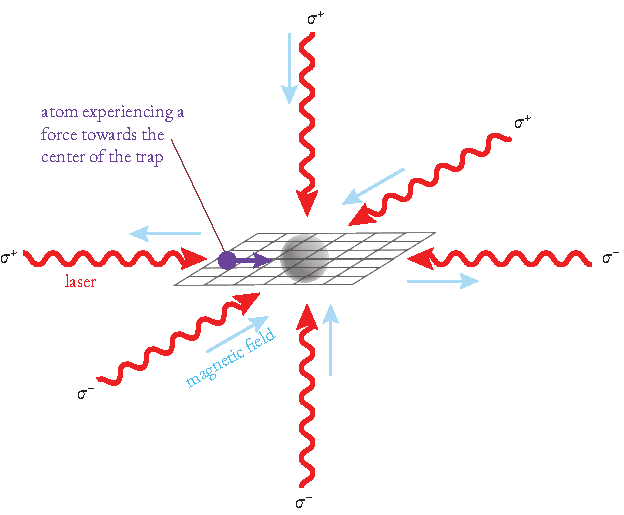
\includegraphics[]{\imagepath/restoring_on_opposite_sides_schematic/restoring_on_opposite_sides_schematic.pdf}
    \caption{Two-dimensional schematic of creation of restoring forces: Due to the magnetic gradient and the Zeeman effect, on each side of the trap, different transitions between magnetic sublevels are on resonance. Assigning different helicity of circular polarization to counter-propagating lasers, atoms only sense a scattering force in the direction of the trap center.}\label{fig:restoring_on_opposite_sides_schematic}
\end{figure} 

\begin{figure}
    \centering
    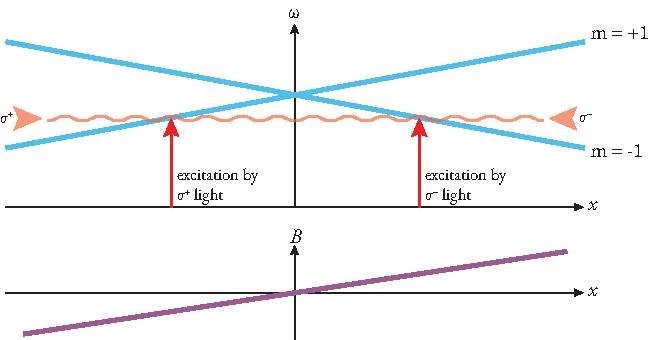
\includegraphics[]{\imagepath/detuning_and_selection_rules_schematic/detuning_and_selection_rules_schematic.pdf}
    \caption{One-dimensional schematic of selection rules and detunings of the laser beams: On both sides of the trap different transitions between magnetic sublevels are resonant with the red-detuned trap light. Due to the polarization-dependent selection rules, only one of the two counter-propagating beams is resonant on each side of the trap which sets the direction of momentum transfer between the light and the atoms. E.g. on the left center, the $\Ket{m = +1}$ state is closer to resonance. Only the $\sigma^+$ light coming from the left can excite this state, hence atoms on the left of the trap mostly acquire moment to the right, i.e. the trap center.}
    \label{fig:detuning_and_selection_rules_schematic}
\end{figure}

Note that the helicity of the polarization is given with respect to the (arbitrary, but fixed) quantization axis of the atoms. As the laser beams in each pair counter-propagate, one of them points to in and one against the quantization axis. The circular polarization with respect to their respective propagation direction is hence the same for both laser beams in a pair (both $\KetText{R}$ or both $\KetText{L}$, depending on the direction of the gradient field).


Similarly to the optical molasses consideration, in the magneto-optical trap the scattering forces can be linearized \todo{Under which condition?} (here again for one dimension)~\cite{foot_atomic_2005}:
\begin{equation}\label{eq:mot_force}
    \begin{split}
        F_\text{MOT} &= F_\text{scatter}^{\sigma^+}(\omega_\text{laser} - \omega_\text{transition}(q) - kv \cos \theta) + F_\text{scatter}^{\sigma^-}(\omega_\text{laser} - \omega_\text{transition}(q) + kv \cos \theta)\\
        &= -2 \pdv{F_\text{scatter}}{\omega} k\cos \theta v + 2 \pdv{F_\text{scatter}}{\omega_0} \beta q  \equiv - (\alpha \cos \theta) v - \frac{\alpha \beta}{k} q
    \end{split}
\end{equation}
This shows how a magneto-optical trap combines the friction force $-(\alpha \cos \theta) v$ for slowing down atoms and the trapping force $- \frac{\alpha \beta}{k} q$ confining the atoms to a trap center.

\todo{Maybe add 3D plot with v, z, F axes.}

\paragraph{Characteristic Quantities and Benchmarks}
Important technical quantities that need to be adjusted for optimizing the performance of a MOT include:
\begin{itemize}
    \item laser intensities $I_\text{cooler}$ and $I_\text{repumper}$
    \item laser detunings with respect to the transition wavelength $\delta_\text{cooler}$ and $\delta_\text{repumper}$
    \item the angle $\theta$ of the atomic beam with respect to the cooling laser beams
    \item magnetic gradient $\pdv{B}{q}$
\end{itemize}

These quantities might also be varied over one trapping cycle, e.g. for compressing the trap and cooling the atoms further down by decreasing the laser intensity and the laser detuning and increasing the magnetic gradient.

The magneto-optical trap can be benchmarked by, among others, the following quantities:
\begin{itemize}
    \item The radius $r_\text{trap}$ of the trapping region where the atoms are slowed  is on the order of the size of the trapping beams: $r_\text{trap} \approx w$.
    \item The trap size is also limited by the distance $r_\text{resonance}$ from the trap center where the trapping beams become resonant due to the Zeeman shift, thus $\omega_\text{laser} - \omega_\text{transition} - \vec k \vec v = \frac{g \mu_\text{B}}{\hbar} \pdv{B}{q} r_\text{resonance}$~\cite{tiecke_high-flux_2009}:
    \begin{align}\label{eq:resonance_radius}
        r_\text{resonance}(\vec v) = \frac{\hbar}{g \mu_\text{B}} \left(\pdv{B}{q}\right)^{-1} \left(\omega_\text{laser} - \omega_\text{transition} - \vec k \vec v\right)
    \end{align}
     At larger distances from the trap, the trapping light is blue detuned and thus accelerating, hence slowing of atoms of velocity $\vec v$ only occurs within a distance of $r_\text{resonance}(\vec v)$. In a one-dimensional consideration with $\vec k \vec v = - kv \cos\theta$, one can deduce a maximum speed at which atoms entering the trap can still be on resonance at the outermost position $r_\text{trap}$~\cite{tiecke_high-flux_2009}:
    \begin{align}\label{eq:resonance_velocity}
        v_\text{max, resonance} \approx \frac{1}{k \cos \theta}
        \left(
            \frac{g \mu_\text{B}}{\hbar} \pdv{B}{q} r_\text{trap} - \left(\omega_\text{laser} - \omega_\text{transition}\right)
        \right)
    \end{align}
    Assuming that the slowing force is large, one can assume that, on the way towards the trap center, the atoms are kept on resonance with the (due to the magnetic gradient) ever less detuned trapping light. In this case, $v_\text{max, resonance}$ can give the order of magnitude of the capture velocity of the trap~\cite{tiecke_high-flux_2009}.
    \item Additionally, one can estimate a maximum velocity $v_\text{max, capture}$ such that the atoms entering the trap are decelerated to standstill within the length $2r_\text{trap}$ of the trap. This would require that their kinetic energy $\frac{1}{2}mv^2$ be dissipated by the cooling force performing the mechanical work $\int F_\text{MOT}(q) \dd{q}$. In case of high radiation pressure, this can be approximated with the maximum scattering force $F_\text{scatter, max}(q) = \frac{\hbar k \Gamma}{2}$ being constant over the whole trap, leading to the following capture velocity \cite{lunden_enhancing_2020}:
    \begin{align}\label{eq:capture_velocity_high}
        v_\text{capture, max}^\text{high} \approx \sqrt{\frac{\hbar k \Gamma \cdot 2 r_\text{trap}}{m}}.
    \end{align}
     For a lower scattering force ($s_0 \ll 1$, see~\eqref{eq:mot_force}), the work is $\int F_\text{MOT}(q)\dd{q}= \int (-\alpha \cos \theta v(q) - \frac{\alpha\beta}{k}q) \dd{q} = - \int \alpha \cos \theta v(q) \dd{q}$ (see~\eqref{eq:mot_force}):
    \begin{align}
            v_\text{max, capture}^\text{low}
            = \sqrt{\frac{2}{m} \int\limits_{-r_\text{trap}}^{+r_\text{trap}} F_\text{MOT}(q) \dd{q}} 
            \approx \sqrt{\frac{2}{m} \alpha \cos \theta \cdot \frac{v_\text{max, capture}}{2} \cdot 2r_\text{trap}}
    \end{align}
    where the integral over the velocity was estimated as $\int\limits_{-r_\text{trap}}^{+r_\text{trap}}  v(q) \dd{q} \approx \frac{v_\text{max}}{2} \cdot 2r_\text{trap}$, assuming that the velocity in the trap is reduced at a constant rate until standstill. The capture velocity is then estimated as
    \begin{align}\label{eq:capture_velocity_low}
        v_\text{max, capture}^\text{low} \approx \frac{2 \alpha \cos \theta ~ r_\text{trap}}{m}.
    \end{align}
    Figure \ref{fig:capture_velocity_comparison} compares the two estimations of the capture velocity. For small saturation intensities, $v_\text{max, capture}^\text{low}$ takes into consideration that the slowing force is weak, hence only slow atoms can be brought to standstill in the trap. For higher saturation intensities, where it loses applicability, $v_\text{max, capture}^\text{low}$ approaches $v_\text{max, capture}^\text{high}$ setting the upper bound of the capture velocity.
    \begin{figure}
        \centering
        \begin{pgfpicture}
            \pgftext{%% Creator: Matplotlib, PGF backend
%%
%% To include the figure in your LaTeX document, write
%%   \input{<filename>.pgf}
%%
%% Make sure the required packages are loaded in your preamble
%%   \usepackage{pgf}
%%
%% Also ensure that all the required font packages are loaded; for instance,
%% the lmodern package is sometimes necessary when using math font.
%%   \usepackage{lmodern}
%%
%% Figures using additional raster images can only be included by \input if
%% they are in the same directory as the main LaTeX file. For loading figures
%% from other directories you can use the `import` package
%%   \usepackage{import}
%%
%% and then include the figures with
%%   \import{<path to file>}{<filename>.pgf}
%%
%% Matplotlib used the following preamble
%%   \usepackage{fontspec}
%%   \setmainfont{DejaVuSerif.ttf}[Path=\detokenize{/home/max/.local/lib/python3.8/site-packages/matplotlib/mpl-data/fonts/ttf/}]
%%   \setsansfont{DejaVuSans.ttf}[Path=\detokenize{/home/max/.local/lib/python3.8/site-packages/matplotlib/mpl-data/fonts/ttf/}]
%%   \setmonofont{DejaVuSansMono.ttf}[Path=\detokenize{/home/max/.local/lib/python3.8/site-packages/matplotlib/mpl-data/fonts/ttf/}]
%%
\begingroup%
\makeatletter%
\begin{pgfpicture}%
\pgfpathrectangle{\pgfpointorigin}{\pgfqpoint{3.686219in}{1.807319in}}%
\pgfusepath{use as bounding box, clip}%
\begin{pgfscope}%
\pgfsetbuttcap%
\pgfsetmiterjoin%
\definecolor{currentfill}{rgb}{1.000000,1.000000,1.000000}%
\pgfsetfillcolor{currentfill}%
\pgfsetlinewidth{0.000000pt}%
\definecolor{currentstroke}{rgb}{1.000000,1.000000,1.000000}%
\pgfsetstrokecolor{currentstroke}%
\pgfsetdash{}{0pt}%
\pgfpathmoveto{\pgfqpoint{0.000000in}{0.000000in}}%
\pgfpathlineto{\pgfqpoint{3.686219in}{0.000000in}}%
\pgfpathlineto{\pgfqpoint{3.686219in}{1.807319in}}%
\pgfpathlineto{\pgfqpoint{0.000000in}{1.807319in}}%
\pgfpathlineto{\pgfqpoint{0.000000in}{0.000000in}}%
\pgfpathclose%
\pgfusepath{fill}%
\end{pgfscope}%
\begin{pgfscope}%
\pgfsetbuttcap%
\pgfsetmiterjoin%
\definecolor{currentfill}{rgb}{1.000000,1.000000,1.000000}%
\pgfsetfillcolor{currentfill}%
\pgfsetlinewidth{0.000000pt}%
\definecolor{currentstroke}{rgb}{0.000000,0.000000,0.000000}%
\pgfsetstrokecolor{currentstroke}%
\pgfsetstrokeopacity{0.000000}%
\pgfsetdash{}{0pt}%
\pgfpathmoveto{\pgfqpoint{0.535038in}{0.494721in}}%
\pgfpathlineto{\pgfqpoint{3.586219in}{0.494721in}}%
\pgfpathlineto{\pgfqpoint{3.586219in}{1.707319in}}%
\pgfpathlineto{\pgfqpoint{0.535038in}{1.707319in}}%
\pgfpathlineto{\pgfqpoint{0.535038in}{0.494721in}}%
\pgfpathclose%
\pgfusepath{fill}%
\end{pgfscope}%
\begin{pgfscope}%
\pgfpathrectangle{\pgfqpoint{0.535038in}{0.494721in}}{\pgfqpoint{3.051181in}{1.212598in}}%
\pgfusepath{clip}%
\pgfsetrectcap%
\pgfsetroundjoin%
\pgfsetlinewidth{0.803000pt}%
\definecolor{currentstroke}{rgb}{0.690196,0.690196,0.690196}%
\pgfsetstrokecolor{currentstroke}%
\pgfsetdash{}{0pt}%
\pgfpathmoveto{\pgfqpoint{0.673728in}{0.494721in}}%
\pgfpathlineto{\pgfqpoint{0.673728in}{1.707319in}}%
\pgfusepath{stroke}%
\end{pgfscope}%
\begin{pgfscope}%
\pgfsetbuttcap%
\pgfsetroundjoin%
\definecolor{currentfill}{rgb}{0.000000,0.000000,0.000000}%
\pgfsetfillcolor{currentfill}%
\pgfsetlinewidth{0.803000pt}%
\definecolor{currentstroke}{rgb}{0.000000,0.000000,0.000000}%
\pgfsetstrokecolor{currentstroke}%
\pgfsetdash{}{0pt}%
\pgfsys@defobject{currentmarker}{\pgfqpoint{0.000000in}{-0.048611in}}{\pgfqpoint{0.000000in}{0.000000in}}{%
\pgfpathmoveto{\pgfqpoint{0.000000in}{0.000000in}}%
\pgfpathlineto{\pgfqpoint{0.000000in}{-0.048611in}}%
\pgfusepath{stroke,fill}%
}%
\begin{pgfscope}%
\pgfsys@transformshift{0.673728in}{0.494721in}%
\pgfsys@useobject{currentmarker}{}%
\end{pgfscope}%
\end{pgfscope}%
\begin{pgfscope}%
\definecolor{textcolor}{rgb}{0.000000,0.000000,0.000000}%
\pgfsetstrokecolor{textcolor}%
\pgfsetfillcolor{textcolor}%
\pgftext[x=0.673728in,y=0.397499in,,top]{\color{textcolor}\rmfamily\fontsize{9.000000}{10.800000}\selectfont 0.0}%
\end{pgfscope}%
\begin{pgfscope}%
\pgfpathrectangle{\pgfqpoint{0.535038in}{0.494721in}}{\pgfqpoint{3.051181in}{1.212598in}}%
\pgfusepath{clip}%
\pgfsetrectcap%
\pgfsetroundjoin%
\pgfsetlinewidth{0.803000pt}%
\definecolor{currentstroke}{rgb}{0.690196,0.690196,0.690196}%
\pgfsetstrokecolor{currentstroke}%
\pgfsetdash{}{0pt}%
\pgfpathmoveto{\pgfqpoint{1.100467in}{0.494721in}}%
\pgfpathlineto{\pgfqpoint{1.100467in}{1.707319in}}%
\pgfusepath{stroke}%
\end{pgfscope}%
\begin{pgfscope}%
\pgfsetbuttcap%
\pgfsetroundjoin%
\definecolor{currentfill}{rgb}{0.000000,0.000000,0.000000}%
\pgfsetfillcolor{currentfill}%
\pgfsetlinewidth{0.803000pt}%
\definecolor{currentstroke}{rgb}{0.000000,0.000000,0.000000}%
\pgfsetstrokecolor{currentstroke}%
\pgfsetdash{}{0pt}%
\pgfsys@defobject{currentmarker}{\pgfqpoint{0.000000in}{-0.048611in}}{\pgfqpoint{0.000000in}{0.000000in}}{%
\pgfpathmoveto{\pgfqpoint{0.000000in}{0.000000in}}%
\pgfpathlineto{\pgfqpoint{0.000000in}{-0.048611in}}%
\pgfusepath{stroke,fill}%
}%
\begin{pgfscope}%
\pgfsys@transformshift{1.100467in}{0.494721in}%
\pgfsys@useobject{currentmarker}{}%
\end{pgfscope}%
\end{pgfscope}%
\begin{pgfscope}%
\definecolor{textcolor}{rgb}{0.000000,0.000000,0.000000}%
\pgfsetstrokecolor{textcolor}%
\pgfsetfillcolor{textcolor}%
\pgftext[x=1.100467in,y=0.397499in,,top]{\color{textcolor}\rmfamily\fontsize{9.000000}{10.800000}\selectfont 0.2}%
\end{pgfscope}%
\begin{pgfscope}%
\pgfpathrectangle{\pgfqpoint{0.535038in}{0.494721in}}{\pgfqpoint{3.051181in}{1.212598in}}%
\pgfusepath{clip}%
\pgfsetrectcap%
\pgfsetroundjoin%
\pgfsetlinewidth{0.803000pt}%
\definecolor{currentstroke}{rgb}{0.690196,0.690196,0.690196}%
\pgfsetstrokecolor{currentstroke}%
\pgfsetdash{}{0pt}%
\pgfpathmoveto{\pgfqpoint{1.527205in}{0.494721in}}%
\pgfpathlineto{\pgfqpoint{1.527205in}{1.707319in}}%
\pgfusepath{stroke}%
\end{pgfscope}%
\begin{pgfscope}%
\pgfsetbuttcap%
\pgfsetroundjoin%
\definecolor{currentfill}{rgb}{0.000000,0.000000,0.000000}%
\pgfsetfillcolor{currentfill}%
\pgfsetlinewidth{0.803000pt}%
\definecolor{currentstroke}{rgb}{0.000000,0.000000,0.000000}%
\pgfsetstrokecolor{currentstroke}%
\pgfsetdash{}{0pt}%
\pgfsys@defobject{currentmarker}{\pgfqpoint{0.000000in}{-0.048611in}}{\pgfqpoint{0.000000in}{0.000000in}}{%
\pgfpathmoveto{\pgfqpoint{0.000000in}{0.000000in}}%
\pgfpathlineto{\pgfqpoint{0.000000in}{-0.048611in}}%
\pgfusepath{stroke,fill}%
}%
\begin{pgfscope}%
\pgfsys@transformshift{1.527205in}{0.494721in}%
\pgfsys@useobject{currentmarker}{}%
\end{pgfscope}%
\end{pgfscope}%
\begin{pgfscope}%
\definecolor{textcolor}{rgb}{0.000000,0.000000,0.000000}%
\pgfsetstrokecolor{textcolor}%
\pgfsetfillcolor{textcolor}%
\pgftext[x=1.527205in,y=0.397499in,,top]{\color{textcolor}\rmfamily\fontsize{9.000000}{10.800000}\selectfont 0.4}%
\end{pgfscope}%
\begin{pgfscope}%
\pgfpathrectangle{\pgfqpoint{0.535038in}{0.494721in}}{\pgfqpoint{3.051181in}{1.212598in}}%
\pgfusepath{clip}%
\pgfsetrectcap%
\pgfsetroundjoin%
\pgfsetlinewidth{0.803000pt}%
\definecolor{currentstroke}{rgb}{0.690196,0.690196,0.690196}%
\pgfsetstrokecolor{currentstroke}%
\pgfsetdash{}{0pt}%
\pgfpathmoveto{\pgfqpoint{1.953944in}{0.494721in}}%
\pgfpathlineto{\pgfqpoint{1.953944in}{1.707319in}}%
\pgfusepath{stroke}%
\end{pgfscope}%
\begin{pgfscope}%
\pgfsetbuttcap%
\pgfsetroundjoin%
\definecolor{currentfill}{rgb}{0.000000,0.000000,0.000000}%
\pgfsetfillcolor{currentfill}%
\pgfsetlinewidth{0.803000pt}%
\definecolor{currentstroke}{rgb}{0.000000,0.000000,0.000000}%
\pgfsetstrokecolor{currentstroke}%
\pgfsetdash{}{0pt}%
\pgfsys@defobject{currentmarker}{\pgfqpoint{0.000000in}{-0.048611in}}{\pgfqpoint{0.000000in}{0.000000in}}{%
\pgfpathmoveto{\pgfqpoint{0.000000in}{0.000000in}}%
\pgfpathlineto{\pgfqpoint{0.000000in}{-0.048611in}}%
\pgfusepath{stroke,fill}%
}%
\begin{pgfscope}%
\pgfsys@transformshift{1.953944in}{0.494721in}%
\pgfsys@useobject{currentmarker}{}%
\end{pgfscope}%
\end{pgfscope}%
\begin{pgfscope}%
\definecolor{textcolor}{rgb}{0.000000,0.000000,0.000000}%
\pgfsetstrokecolor{textcolor}%
\pgfsetfillcolor{textcolor}%
\pgftext[x=1.953944in,y=0.397499in,,top]{\color{textcolor}\rmfamily\fontsize{9.000000}{10.800000}\selectfont 0.6}%
\end{pgfscope}%
\begin{pgfscope}%
\pgfpathrectangle{\pgfqpoint{0.535038in}{0.494721in}}{\pgfqpoint{3.051181in}{1.212598in}}%
\pgfusepath{clip}%
\pgfsetrectcap%
\pgfsetroundjoin%
\pgfsetlinewidth{0.803000pt}%
\definecolor{currentstroke}{rgb}{0.690196,0.690196,0.690196}%
\pgfsetstrokecolor{currentstroke}%
\pgfsetdash{}{0pt}%
\pgfpathmoveto{\pgfqpoint{2.380683in}{0.494721in}}%
\pgfpathlineto{\pgfqpoint{2.380683in}{1.707319in}}%
\pgfusepath{stroke}%
\end{pgfscope}%
\begin{pgfscope}%
\pgfsetbuttcap%
\pgfsetroundjoin%
\definecolor{currentfill}{rgb}{0.000000,0.000000,0.000000}%
\pgfsetfillcolor{currentfill}%
\pgfsetlinewidth{0.803000pt}%
\definecolor{currentstroke}{rgb}{0.000000,0.000000,0.000000}%
\pgfsetstrokecolor{currentstroke}%
\pgfsetdash{}{0pt}%
\pgfsys@defobject{currentmarker}{\pgfqpoint{0.000000in}{-0.048611in}}{\pgfqpoint{0.000000in}{0.000000in}}{%
\pgfpathmoveto{\pgfqpoint{0.000000in}{0.000000in}}%
\pgfpathlineto{\pgfqpoint{0.000000in}{-0.048611in}}%
\pgfusepath{stroke,fill}%
}%
\begin{pgfscope}%
\pgfsys@transformshift{2.380683in}{0.494721in}%
\pgfsys@useobject{currentmarker}{}%
\end{pgfscope}%
\end{pgfscope}%
\begin{pgfscope}%
\definecolor{textcolor}{rgb}{0.000000,0.000000,0.000000}%
\pgfsetstrokecolor{textcolor}%
\pgfsetfillcolor{textcolor}%
\pgftext[x=2.380683in,y=0.397499in,,top]{\color{textcolor}\rmfamily\fontsize{9.000000}{10.800000}\selectfont 0.8}%
\end{pgfscope}%
\begin{pgfscope}%
\pgfpathrectangle{\pgfqpoint{0.535038in}{0.494721in}}{\pgfqpoint{3.051181in}{1.212598in}}%
\pgfusepath{clip}%
\pgfsetrectcap%
\pgfsetroundjoin%
\pgfsetlinewidth{0.803000pt}%
\definecolor{currentstroke}{rgb}{0.690196,0.690196,0.690196}%
\pgfsetstrokecolor{currentstroke}%
\pgfsetdash{}{0pt}%
\pgfpathmoveto{\pgfqpoint{2.807421in}{0.494721in}}%
\pgfpathlineto{\pgfqpoint{2.807421in}{1.707319in}}%
\pgfusepath{stroke}%
\end{pgfscope}%
\begin{pgfscope}%
\pgfsetbuttcap%
\pgfsetroundjoin%
\definecolor{currentfill}{rgb}{0.000000,0.000000,0.000000}%
\pgfsetfillcolor{currentfill}%
\pgfsetlinewidth{0.803000pt}%
\definecolor{currentstroke}{rgb}{0.000000,0.000000,0.000000}%
\pgfsetstrokecolor{currentstroke}%
\pgfsetdash{}{0pt}%
\pgfsys@defobject{currentmarker}{\pgfqpoint{0.000000in}{-0.048611in}}{\pgfqpoint{0.000000in}{0.000000in}}{%
\pgfpathmoveto{\pgfqpoint{0.000000in}{0.000000in}}%
\pgfpathlineto{\pgfqpoint{0.000000in}{-0.048611in}}%
\pgfusepath{stroke,fill}%
}%
\begin{pgfscope}%
\pgfsys@transformshift{2.807421in}{0.494721in}%
\pgfsys@useobject{currentmarker}{}%
\end{pgfscope}%
\end{pgfscope}%
\begin{pgfscope}%
\definecolor{textcolor}{rgb}{0.000000,0.000000,0.000000}%
\pgfsetstrokecolor{textcolor}%
\pgfsetfillcolor{textcolor}%
\pgftext[x=2.807421in,y=0.397499in,,top]{\color{textcolor}\rmfamily\fontsize{9.000000}{10.800000}\selectfont 1.0}%
\end{pgfscope}%
\begin{pgfscope}%
\pgfpathrectangle{\pgfqpoint{0.535038in}{0.494721in}}{\pgfqpoint{3.051181in}{1.212598in}}%
\pgfusepath{clip}%
\pgfsetrectcap%
\pgfsetroundjoin%
\pgfsetlinewidth{0.803000pt}%
\definecolor{currentstroke}{rgb}{0.690196,0.690196,0.690196}%
\pgfsetstrokecolor{currentstroke}%
\pgfsetdash{}{0pt}%
\pgfpathmoveto{\pgfqpoint{3.234160in}{0.494721in}}%
\pgfpathlineto{\pgfqpoint{3.234160in}{1.707319in}}%
\pgfusepath{stroke}%
\end{pgfscope}%
\begin{pgfscope}%
\pgfsetbuttcap%
\pgfsetroundjoin%
\definecolor{currentfill}{rgb}{0.000000,0.000000,0.000000}%
\pgfsetfillcolor{currentfill}%
\pgfsetlinewidth{0.803000pt}%
\definecolor{currentstroke}{rgb}{0.000000,0.000000,0.000000}%
\pgfsetstrokecolor{currentstroke}%
\pgfsetdash{}{0pt}%
\pgfsys@defobject{currentmarker}{\pgfqpoint{0.000000in}{-0.048611in}}{\pgfqpoint{0.000000in}{0.000000in}}{%
\pgfpathmoveto{\pgfqpoint{0.000000in}{0.000000in}}%
\pgfpathlineto{\pgfqpoint{0.000000in}{-0.048611in}}%
\pgfusepath{stroke,fill}%
}%
\begin{pgfscope}%
\pgfsys@transformshift{3.234160in}{0.494721in}%
\pgfsys@useobject{currentmarker}{}%
\end{pgfscope}%
\end{pgfscope}%
\begin{pgfscope}%
\definecolor{textcolor}{rgb}{0.000000,0.000000,0.000000}%
\pgfsetstrokecolor{textcolor}%
\pgfsetfillcolor{textcolor}%
\pgftext[x=3.234160in,y=0.397499in,,top]{\color{textcolor}\rmfamily\fontsize{9.000000}{10.800000}\selectfont 1.2}%
\end{pgfscope}%
\begin{pgfscope}%
\definecolor{textcolor}{rgb}{0.000000,0.000000,0.000000}%
\pgfsetstrokecolor{textcolor}%
\pgfsetfillcolor{textcolor}%
\pgftext[x=2.060629in,y=0.220972in,,top]{\color{textcolor}\rmfamily\fontsize{9.000000}{10.800000}\selectfont saturation \(\displaystyle s_0\)}%
\end{pgfscope}%
\begin{pgfscope}%
\pgfpathrectangle{\pgfqpoint{0.535038in}{0.494721in}}{\pgfqpoint{3.051181in}{1.212598in}}%
\pgfusepath{clip}%
\pgfsetrectcap%
\pgfsetroundjoin%
\pgfsetlinewidth{0.803000pt}%
\definecolor{currentstroke}{rgb}{0.690196,0.690196,0.690196}%
\pgfsetstrokecolor{currentstroke}%
\pgfsetdash{}{0pt}%
\pgfpathmoveto{\pgfqpoint{0.535038in}{0.549839in}}%
\pgfpathlineto{\pgfqpoint{3.586219in}{0.549839in}}%
\pgfusepath{stroke}%
\end{pgfscope}%
\begin{pgfscope}%
\pgfsetbuttcap%
\pgfsetroundjoin%
\definecolor{currentfill}{rgb}{0.000000,0.000000,0.000000}%
\pgfsetfillcolor{currentfill}%
\pgfsetlinewidth{0.803000pt}%
\definecolor{currentstroke}{rgb}{0.000000,0.000000,0.000000}%
\pgfsetstrokecolor{currentstroke}%
\pgfsetdash{}{0pt}%
\pgfsys@defobject{currentmarker}{\pgfqpoint{-0.048611in}{0.000000in}}{\pgfqpoint{-0.000000in}{0.000000in}}{%
\pgfpathmoveto{\pgfqpoint{-0.000000in}{0.000000in}}%
\pgfpathlineto{\pgfqpoint{-0.048611in}{0.000000in}}%
\pgfusepath{stroke,fill}%
}%
\begin{pgfscope}%
\pgfsys@transformshift{0.535038in}{0.549839in}%
\pgfsys@useobject{currentmarker}{}%
\end{pgfscope}%
\end{pgfscope}%
\begin{pgfscope}%
\definecolor{textcolor}{rgb}{0.000000,0.000000,0.000000}%
\pgfsetstrokecolor{textcolor}%
\pgfsetfillcolor{textcolor}%
\pgftext[x=0.358287in, y=0.502354in, left, base]{\color{textcolor}\rmfamily\fontsize{9.000000}{10.800000}\selectfont 0}%
\end{pgfscope}%
\begin{pgfscope}%
\pgfpathrectangle{\pgfqpoint{0.535038in}{0.494721in}}{\pgfqpoint{3.051181in}{1.212598in}}%
\pgfusepath{clip}%
\pgfsetrectcap%
\pgfsetroundjoin%
\pgfsetlinewidth{0.803000pt}%
\definecolor{currentstroke}{rgb}{0.690196,0.690196,0.690196}%
\pgfsetstrokecolor{currentstroke}%
\pgfsetdash{}{0pt}%
\pgfpathmoveto{\pgfqpoint{0.535038in}{0.855390in}}%
\pgfpathlineto{\pgfqpoint{3.586219in}{0.855390in}}%
\pgfusepath{stroke}%
\end{pgfscope}%
\begin{pgfscope}%
\pgfsetbuttcap%
\pgfsetroundjoin%
\definecolor{currentfill}{rgb}{0.000000,0.000000,0.000000}%
\pgfsetfillcolor{currentfill}%
\pgfsetlinewidth{0.803000pt}%
\definecolor{currentstroke}{rgb}{0.000000,0.000000,0.000000}%
\pgfsetstrokecolor{currentstroke}%
\pgfsetdash{}{0pt}%
\pgfsys@defobject{currentmarker}{\pgfqpoint{-0.048611in}{0.000000in}}{\pgfqpoint{-0.000000in}{0.000000in}}{%
\pgfpathmoveto{\pgfqpoint{-0.000000in}{0.000000in}}%
\pgfpathlineto{\pgfqpoint{-0.048611in}{0.000000in}}%
\pgfusepath{stroke,fill}%
}%
\begin{pgfscope}%
\pgfsys@transformshift{0.535038in}{0.855390in}%
\pgfsys@useobject{currentmarker}{}%
\end{pgfscope}%
\end{pgfscope}%
\begin{pgfscope}%
\definecolor{textcolor}{rgb}{0.000000,0.000000,0.000000}%
\pgfsetstrokecolor{textcolor}%
\pgfsetfillcolor{textcolor}%
\pgftext[x=0.278758in, y=0.807905in, left, base]{\color{textcolor}\rmfamily\fontsize{9.000000}{10.800000}\selectfont 25}%
\end{pgfscope}%
\begin{pgfscope}%
\pgfpathrectangle{\pgfqpoint{0.535038in}{0.494721in}}{\pgfqpoint{3.051181in}{1.212598in}}%
\pgfusepath{clip}%
\pgfsetrectcap%
\pgfsetroundjoin%
\pgfsetlinewidth{0.803000pt}%
\definecolor{currentstroke}{rgb}{0.690196,0.690196,0.690196}%
\pgfsetstrokecolor{currentstroke}%
\pgfsetdash{}{0pt}%
\pgfpathmoveto{\pgfqpoint{0.535038in}{1.160941in}}%
\pgfpathlineto{\pgfqpoint{3.586219in}{1.160941in}}%
\pgfusepath{stroke}%
\end{pgfscope}%
\begin{pgfscope}%
\pgfsetbuttcap%
\pgfsetroundjoin%
\definecolor{currentfill}{rgb}{0.000000,0.000000,0.000000}%
\pgfsetfillcolor{currentfill}%
\pgfsetlinewidth{0.803000pt}%
\definecolor{currentstroke}{rgb}{0.000000,0.000000,0.000000}%
\pgfsetstrokecolor{currentstroke}%
\pgfsetdash{}{0pt}%
\pgfsys@defobject{currentmarker}{\pgfqpoint{-0.048611in}{0.000000in}}{\pgfqpoint{-0.000000in}{0.000000in}}{%
\pgfpathmoveto{\pgfqpoint{-0.000000in}{0.000000in}}%
\pgfpathlineto{\pgfqpoint{-0.048611in}{0.000000in}}%
\pgfusepath{stroke,fill}%
}%
\begin{pgfscope}%
\pgfsys@transformshift{0.535038in}{1.160941in}%
\pgfsys@useobject{currentmarker}{}%
\end{pgfscope}%
\end{pgfscope}%
\begin{pgfscope}%
\definecolor{textcolor}{rgb}{0.000000,0.000000,0.000000}%
\pgfsetstrokecolor{textcolor}%
\pgfsetfillcolor{textcolor}%
\pgftext[x=0.278758in, y=1.113456in, left, base]{\color{textcolor}\rmfamily\fontsize{9.000000}{10.800000}\selectfont 50}%
\end{pgfscope}%
\begin{pgfscope}%
\pgfpathrectangle{\pgfqpoint{0.535038in}{0.494721in}}{\pgfqpoint{3.051181in}{1.212598in}}%
\pgfusepath{clip}%
\pgfsetrectcap%
\pgfsetroundjoin%
\pgfsetlinewidth{0.803000pt}%
\definecolor{currentstroke}{rgb}{0.690196,0.690196,0.690196}%
\pgfsetstrokecolor{currentstroke}%
\pgfsetdash{}{0pt}%
\pgfpathmoveto{\pgfqpoint{0.535038in}{1.466492in}}%
\pgfpathlineto{\pgfqpoint{3.586219in}{1.466492in}}%
\pgfusepath{stroke}%
\end{pgfscope}%
\begin{pgfscope}%
\pgfsetbuttcap%
\pgfsetroundjoin%
\definecolor{currentfill}{rgb}{0.000000,0.000000,0.000000}%
\pgfsetfillcolor{currentfill}%
\pgfsetlinewidth{0.803000pt}%
\definecolor{currentstroke}{rgb}{0.000000,0.000000,0.000000}%
\pgfsetstrokecolor{currentstroke}%
\pgfsetdash{}{0pt}%
\pgfsys@defobject{currentmarker}{\pgfqpoint{-0.048611in}{0.000000in}}{\pgfqpoint{-0.000000in}{0.000000in}}{%
\pgfpathmoveto{\pgfqpoint{-0.000000in}{0.000000in}}%
\pgfpathlineto{\pgfqpoint{-0.048611in}{0.000000in}}%
\pgfusepath{stroke,fill}%
}%
\begin{pgfscope}%
\pgfsys@transformshift{0.535038in}{1.466492in}%
\pgfsys@useobject{currentmarker}{}%
\end{pgfscope}%
\end{pgfscope}%
\begin{pgfscope}%
\definecolor{textcolor}{rgb}{0.000000,0.000000,0.000000}%
\pgfsetstrokecolor{textcolor}%
\pgfsetfillcolor{textcolor}%
\pgftext[x=0.278758in, y=1.419007in, left, base]{\color{textcolor}\rmfamily\fontsize{9.000000}{10.800000}\selectfont 75}%
\end{pgfscope}%
\begin{pgfscope}%
\definecolor{textcolor}{rgb}{0.000000,0.000000,0.000000}%
\pgfsetstrokecolor{textcolor}%
\pgfsetfillcolor{textcolor}%
\pgftext[x=0.223203in,y=1.101020in,,bottom,rotate=90.000000]{\color{textcolor}\rmfamily\fontsize{9.000000}{10.800000}\selectfont \(\displaystyle v_\mathrm{max, capture}\) in m/s}%
\end{pgfscope}%
\begin{pgfscope}%
\pgfpathrectangle{\pgfqpoint{0.535038in}{0.494721in}}{\pgfqpoint{3.051181in}{1.212598in}}%
\pgfusepath{clip}%
\pgfsetrectcap%
\pgfsetroundjoin%
\pgfsetlinewidth{1.505625pt}%
\definecolor{currentstroke}{rgb}{1.000000,0.000000,0.000000}%
\pgfsetstrokecolor{currentstroke}%
\pgfsetdash{}{0pt}%
\pgfpathmoveto{\pgfqpoint{0.673728in}{1.652201in}}%
\pgfpathlineto{\pgfqpoint{0.701746in}{1.652201in}}%
\pgfpathlineto{\pgfqpoint{0.729764in}{1.652201in}}%
\pgfpathlineto{\pgfqpoint{0.757783in}{1.652201in}}%
\pgfpathlineto{\pgfqpoint{0.785801in}{1.652201in}}%
\pgfpathlineto{\pgfqpoint{0.813819in}{1.652201in}}%
\pgfpathlineto{\pgfqpoint{0.841837in}{1.652201in}}%
\pgfpathlineto{\pgfqpoint{0.869855in}{1.652201in}}%
\pgfpathlineto{\pgfqpoint{0.897874in}{1.652201in}}%
\pgfpathlineto{\pgfqpoint{0.925892in}{1.652201in}}%
\pgfpathlineto{\pgfqpoint{0.953910in}{1.652201in}}%
\pgfpathlineto{\pgfqpoint{0.981928in}{1.652201in}}%
\pgfpathlineto{\pgfqpoint{1.009946in}{1.652201in}}%
\pgfpathlineto{\pgfqpoint{1.037965in}{1.652201in}}%
\pgfpathlineto{\pgfqpoint{1.065983in}{1.652201in}}%
\pgfpathlineto{\pgfqpoint{1.094001in}{1.652201in}}%
\pgfpathlineto{\pgfqpoint{1.122019in}{1.652201in}}%
\pgfpathlineto{\pgfqpoint{1.150037in}{1.652201in}}%
\pgfpathlineto{\pgfqpoint{1.178056in}{1.652201in}}%
\pgfpathlineto{\pgfqpoint{1.206074in}{1.652201in}}%
\pgfpathlineto{\pgfqpoint{1.234092in}{1.652201in}}%
\pgfpathlineto{\pgfqpoint{1.262110in}{1.652201in}}%
\pgfpathlineto{\pgfqpoint{1.290128in}{1.652201in}}%
\pgfpathlineto{\pgfqpoint{1.318147in}{1.652201in}}%
\pgfpathlineto{\pgfqpoint{1.346165in}{1.652201in}}%
\pgfpathlineto{\pgfqpoint{1.374183in}{1.652201in}}%
\pgfpathlineto{\pgfqpoint{1.402201in}{1.652201in}}%
\pgfpathlineto{\pgfqpoint{1.430219in}{1.652201in}}%
\pgfpathlineto{\pgfqpoint{1.458237in}{1.652201in}}%
\pgfpathlineto{\pgfqpoint{1.486256in}{1.652201in}}%
\pgfpathlineto{\pgfqpoint{1.514274in}{1.652201in}}%
\pgfpathlineto{\pgfqpoint{1.542292in}{1.652201in}}%
\pgfpathlineto{\pgfqpoint{1.570310in}{1.652201in}}%
\pgfpathlineto{\pgfqpoint{1.598328in}{1.652201in}}%
\pgfpathlineto{\pgfqpoint{1.626347in}{1.652201in}}%
\pgfpathlineto{\pgfqpoint{1.654365in}{1.652201in}}%
\pgfpathlineto{\pgfqpoint{1.682383in}{1.652201in}}%
\pgfpathlineto{\pgfqpoint{1.710401in}{1.652201in}}%
\pgfpathlineto{\pgfqpoint{1.738419in}{1.652201in}}%
\pgfpathlineto{\pgfqpoint{1.766438in}{1.652201in}}%
\pgfpathlineto{\pgfqpoint{1.794456in}{1.652201in}}%
\pgfpathlineto{\pgfqpoint{1.822474in}{1.652201in}}%
\pgfpathlineto{\pgfqpoint{1.850492in}{1.652201in}}%
\pgfpathlineto{\pgfqpoint{1.878510in}{1.652201in}}%
\pgfpathlineto{\pgfqpoint{1.906529in}{1.652201in}}%
\pgfpathlineto{\pgfqpoint{1.934547in}{1.652201in}}%
\pgfpathlineto{\pgfqpoint{1.962565in}{1.652201in}}%
\pgfpathlineto{\pgfqpoint{1.990583in}{1.652201in}}%
\pgfpathlineto{\pgfqpoint{2.018601in}{1.652201in}}%
\pgfpathlineto{\pgfqpoint{2.046620in}{1.652201in}}%
\pgfpathlineto{\pgfqpoint{2.074638in}{1.652201in}}%
\pgfpathlineto{\pgfqpoint{2.102656in}{1.652201in}}%
\pgfpathlineto{\pgfqpoint{2.130674in}{1.652201in}}%
\pgfpathlineto{\pgfqpoint{2.158692in}{1.652201in}}%
\pgfpathlineto{\pgfqpoint{2.186710in}{1.652201in}}%
\pgfpathlineto{\pgfqpoint{2.214729in}{1.652201in}}%
\pgfpathlineto{\pgfqpoint{2.242747in}{1.652201in}}%
\pgfpathlineto{\pgfqpoint{2.270765in}{1.652201in}}%
\pgfpathlineto{\pgfqpoint{2.298783in}{1.652201in}}%
\pgfpathlineto{\pgfqpoint{2.326801in}{1.652201in}}%
\pgfpathlineto{\pgfqpoint{2.354820in}{1.652201in}}%
\pgfpathlineto{\pgfqpoint{2.382838in}{1.652201in}}%
\pgfpathlineto{\pgfqpoint{2.410856in}{1.652201in}}%
\pgfpathlineto{\pgfqpoint{2.438874in}{1.652201in}}%
\pgfpathlineto{\pgfqpoint{2.466892in}{1.652201in}}%
\pgfpathlineto{\pgfqpoint{2.494911in}{1.652201in}}%
\pgfpathlineto{\pgfqpoint{2.522929in}{1.652201in}}%
\pgfpathlineto{\pgfqpoint{2.550947in}{1.652201in}}%
\pgfpathlineto{\pgfqpoint{2.578965in}{1.652201in}}%
\pgfpathlineto{\pgfqpoint{2.606983in}{1.652201in}}%
\pgfpathlineto{\pgfqpoint{2.635002in}{1.652201in}}%
\pgfpathlineto{\pgfqpoint{2.663020in}{1.652201in}}%
\pgfpathlineto{\pgfqpoint{2.691038in}{1.652201in}}%
\pgfpathlineto{\pgfqpoint{2.719056in}{1.652201in}}%
\pgfpathlineto{\pgfqpoint{2.747074in}{1.652201in}}%
\pgfpathlineto{\pgfqpoint{2.775093in}{1.652201in}}%
\pgfpathlineto{\pgfqpoint{2.803111in}{1.652201in}}%
\pgfpathlineto{\pgfqpoint{2.831129in}{1.652201in}}%
\pgfpathlineto{\pgfqpoint{2.859147in}{1.652201in}}%
\pgfpathlineto{\pgfqpoint{2.887165in}{1.652201in}}%
\pgfpathlineto{\pgfqpoint{2.915183in}{1.652201in}}%
\pgfpathlineto{\pgfqpoint{2.943202in}{1.652201in}}%
\pgfpathlineto{\pgfqpoint{2.971220in}{1.652201in}}%
\pgfpathlineto{\pgfqpoint{2.999238in}{1.652201in}}%
\pgfpathlineto{\pgfqpoint{3.027256in}{1.652201in}}%
\pgfpathlineto{\pgfqpoint{3.055274in}{1.652201in}}%
\pgfpathlineto{\pgfqpoint{3.083293in}{1.652201in}}%
\pgfpathlineto{\pgfqpoint{3.111311in}{1.652201in}}%
\pgfpathlineto{\pgfqpoint{3.139329in}{1.652201in}}%
\pgfpathlineto{\pgfqpoint{3.167347in}{1.652201in}}%
\pgfpathlineto{\pgfqpoint{3.195365in}{1.652201in}}%
\pgfpathlineto{\pgfqpoint{3.223384in}{1.652201in}}%
\pgfpathlineto{\pgfqpoint{3.251402in}{1.652201in}}%
\pgfpathlineto{\pgfqpoint{3.279420in}{1.652201in}}%
\pgfpathlineto{\pgfqpoint{3.307438in}{1.652201in}}%
\pgfpathlineto{\pgfqpoint{3.335456in}{1.652201in}}%
\pgfpathlineto{\pgfqpoint{3.363475in}{1.652201in}}%
\pgfpathlineto{\pgfqpoint{3.391493in}{1.652201in}}%
\pgfpathlineto{\pgfqpoint{3.419511in}{1.652201in}}%
\pgfpathlineto{\pgfqpoint{3.447529in}{1.652201in}}%
\pgfusepath{stroke}%
\end{pgfscope}%
\begin{pgfscope}%
\pgfpathrectangle{\pgfqpoint{0.535038in}{0.494721in}}{\pgfqpoint{3.051181in}{1.212598in}}%
\pgfusepath{clip}%
\pgfsetrectcap%
\pgfsetroundjoin%
\pgfsetlinewidth{1.505625pt}%
\definecolor{currentstroke}{rgb}{0.313725,0.741176,0.913725}%
\pgfsetstrokecolor{currentstroke}%
\pgfsetdash{}{0pt}%
\pgfpathmoveto{\pgfqpoint{0.673728in}{0.549839in}}%
\pgfpathlineto{\pgfqpoint{0.701746in}{0.558001in}}%
\pgfpathlineto{\pgfqpoint{0.729764in}{0.566158in}}%
\pgfpathlineto{\pgfqpoint{0.757783in}{0.574311in}}%
\pgfpathlineto{\pgfqpoint{0.785801in}{0.582460in}}%
\pgfpathlineto{\pgfqpoint{0.813819in}{0.590604in}}%
\pgfpathlineto{\pgfqpoint{0.841837in}{0.598745in}}%
\pgfpathlineto{\pgfqpoint{0.869855in}{0.606881in}}%
\pgfpathlineto{\pgfqpoint{0.897874in}{0.615013in}}%
\pgfpathlineto{\pgfqpoint{0.925892in}{0.623141in}}%
\pgfpathlineto{\pgfqpoint{0.953910in}{0.631264in}}%
\pgfpathlineto{\pgfqpoint{0.981928in}{0.639383in}}%
\pgfpathlineto{\pgfqpoint{1.009946in}{0.647498in}}%
\pgfpathlineto{\pgfqpoint{1.037965in}{0.655609in}}%
\pgfpathlineto{\pgfqpoint{1.065983in}{0.663716in}}%
\pgfpathlineto{\pgfqpoint{1.094001in}{0.671818in}}%
\pgfpathlineto{\pgfqpoint{1.122019in}{0.679916in}}%
\pgfpathlineto{\pgfqpoint{1.150037in}{0.688010in}}%
\pgfpathlineto{\pgfqpoint{1.178056in}{0.696100in}}%
\pgfpathlineto{\pgfqpoint{1.206074in}{0.704186in}}%
\pgfpathlineto{\pgfqpoint{1.234092in}{0.712267in}}%
\pgfpathlineto{\pgfqpoint{1.262110in}{0.720344in}}%
\pgfpathlineto{\pgfqpoint{1.290128in}{0.728417in}}%
\pgfpathlineto{\pgfqpoint{1.318147in}{0.736486in}}%
\pgfpathlineto{\pgfqpoint{1.346165in}{0.744551in}}%
\pgfpathlineto{\pgfqpoint{1.374183in}{0.752611in}}%
\pgfpathlineto{\pgfqpoint{1.402201in}{0.760667in}}%
\pgfpathlineto{\pgfqpoint{1.430219in}{0.768719in}}%
\pgfpathlineto{\pgfqpoint{1.458237in}{0.776767in}}%
\pgfpathlineto{\pgfqpoint{1.486256in}{0.784811in}}%
\pgfpathlineto{\pgfqpoint{1.514274in}{0.792850in}}%
\pgfpathlineto{\pgfqpoint{1.542292in}{0.800886in}}%
\pgfpathlineto{\pgfqpoint{1.570310in}{0.808917in}}%
\pgfpathlineto{\pgfqpoint{1.598328in}{0.816944in}}%
\pgfpathlineto{\pgfqpoint{1.626347in}{0.824967in}}%
\pgfpathlineto{\pgfqpoint{1.654365in}{0.832986in}}%
\pgfpathlineto{\pgfqpoint{1.682383in}{0.841000in}}%
\pgfpathlineto{\pgfqpoint{1.710401in}{0.849010in}}%
\pgfpathlineto{\pgfqpoint{1.738419in}{0.857017in}}%
\pgfpathlineto{\pgfqpoint{1.766438in}{0.865019in}}%
\pgfpathlineto{\pgfqpoint{1.794456in}{0.873017in}}%
\pgfpathlineto{\pgfqpoint{1.822474in}{0.881010in}}%
\pgfpathlineto{\pgfqpoint{1.850492in}{0.889000in}}%
\pgfpathlineto{\pgfqpoint{1.878510in}{0.896985in}}%
\pgfpathlineto{\pgfqpoint{1.906529in}{0.904967in}}%
\pgfpathlineto{\pgfqpoint{1.934547in}{0.912944in}}%
\pgfpathlineto{\pgfqpoint{1.962565in}{0.920917in}}%
\pgfpathlineto{\pgfqpoint{1.990583in}{0.928886in}}%
\pgfpathlineto{\pgfqpoint{2.018601in}{0.936851in}}%
\pgfpathlineto{\pgfqpoint{2.046620in}{0.944811in}}%
\pgfpathlineto{\pgfqpoint{2.074638in}{0.952768in}}%
\pgfpathlineto{\pgfqpoint{2.102656in}{0.960720in}}%
\pgfpathlineto{\pgfqpoint{2.130674in}{0.968669in}}%
\pgfpathlineto{\pgfqpoint{2.158692in}{0.976613in}}%
\pgfpathlineto{\pgfqpoint{2.186710in}{0.984553in}}%
\pgfpathlineto{\pgfqpoint{2.214729in}{0.992489in}}%
\pgfpathlineto{\pgfqpoint{2.242747in}{1.000421in}}%
\pgfpathlineto{\pgfqpoint{2.270765in}{1.008349in}}%
\pgfpathlineto{\pgfqpoint{2.298783in}{1.016272in}}%
\pgfpathlineto{\pgfqpoint{2.326801in}{1.024192in}}%
\pgfpathlineto{\pgfqpoint{2.354820in}{1.032107in}}%
\pgfpathlineto{\pgfqpoint{2.382838in}{1.040018in}}%
\pgfpathlineto{\pgfqpoint{2.410856in}{1.047926in}}%
\pgfpathlineto{\pgfqpoint{2.438874in}{1.055829in}}%
\pgfpathlineto{\pgfqpoint{2.466892in}{1.063728in}}%
\pgfpathlineto{\pgfqpoint{2.494911in}{1.071623in}}%
\pgfpathlineto{\pgfqpoint{2.522929in}{1.079514in}}%
\pgfpathlineto{\pgfqpoint{2.550947in}{1.087400in}}%
\pgfpathlineto{\pgfqpoint{2.578965in}{1.095283in}}%
\pgfpathlineto{\pgfqpoint{2.606983in}{1.103162in}}%
\pgfpathlineto{\pgfqpoint{2.635002in}{1.111036in}}%
\pgfpathlineto{\pgfqpoint{2.663020in}{1.118907in}}%
\pgfpathlineto{\pgfqpoint{2.691038in}{1.126773in}}%
\pgfpathlineto{\pgfqpoint{2.719056in}{1.134635in}}%
\pgfpathlineto{\pgfqpoint{2.747074in}{1.142494in}}%
\pgfpathlineto{\pgfqpoint{2.775093in}{1.150348in}}%
\pgfpathlineto{\pgfqpoint{2.803111in}{1.158198in}}%
\pgfpathlineto{\pgfqpoint{2.831129in}{1.166044in}}%
\pgfpathlineto{\pgfqpoint{2.859147in}{1.173886in}}%
\pgfpathlineto{\pgfqpoint{2.887165in}{1.181724in}}%
\pgfpathlineto{\pgfqpoint{2.915183in}{1.189558in}}%
\pgfpathlineto{\pgfqpoint{2.943202in}{1.197388in}}%
\pgfpathlineto{\pgfqpoint{2.971220in}{1.205213in}}%
\pgfpathlineto{\pgfqpoint{2.999238in}{1.213035in}}%
\pgfpathlineto{\pgfqpoint{3.027256in}{1.220853in}}%
\pgfpathlineto{\pgfqpoint{3.055274in}{1.228666in}}%
\pgfpathlineto{\pgfqpoint{3.083293in}{1.236476in}}%
\pgfpathlineto{\pgfqpoint{3.111311in}{1.244282in}}%
\pgfpathlineto{\pgfqpoint{3.139329in}{1.252083in}}%
\pgfpathlineto{\pgfqpoint{3.167347in}{1.259881in}}%
\pgfpathlineto{\pgfqpoint{3.195365in}{1.267674in}}%
\pgfpathlineto{\pgfqpoint{3.223384in}{1.275464in}}%
\pgfpathlineto{\pgfqpoint{3.251402in}{1.283249in}}%
\pgfpathlineto{\pgfqpoint{3.279420in}{1.291030in}}%
\pgfpathlineto{\pgfqpoint{3.307438in}{1.298808in}}%
\pgfpathlineto{\pgfqpoint{3.335456in}{1.306581in}}%
\pgfpathlineto{\pgfqpoint{3.363475in}{1.314350in}}%
\pgfpathlineto{\pgfqpoint{3.391493in}{1.322116in}}%
\pgfpathlineto{\pgfqpoint{3.419511in}{1.329877in}}%
\pgfpathlineto{\pgfqpoint{3.447529in}{1.337634in}}%
\pgfusepath{stroke}%
\end{pgfscope}%
\begin{pgfscope}%
\pgfsetrectcap%
\pgfsetmiterjoin%
\pgfsetlinewidth{0.803000pt}%
\definecolor{currentstroke}{rgb}{0.000000,0.000000,0.000000}%
\pgfsetstrokecolor{currentstroke}%
\pgfsetdash{}{0pt}%
\pgfpathmoveto{\pgfqpoint{0.535038in}{0.494721in}}%
\pgfpathlineto{\pgfqpoint{0.535038in}{1.707319in}}%
\pgfusepath{stroke}%
\end{pgfscope}%
\begin{pgfscope}%
\pgfsetrectcap%
\pgfsetmiterjoin%
\pgfsetlinewidth{0.803000pt}%
\definecolor{currentstroke}{rgb}{0.000000,0.000000,0.000000}%
\pgfsetstrokecolor{currentstroke}%
\pgfsetdash{}{0pt}%
\pgfpathmoveto{\pgfqpoint{3.586219in}{0.494721in}}%
\pgfpathlineto{\pgfqpoint{3.586219in}{1.707319in}}%
\pgfusepath{stroke}%
\end{pgfscope}%
\begin{pgfscope}%
\pgfsetrectcap%
\pgfsetmiterjoin%
\pgfsetlinewidth{0.803000pt}%
\definecolor{currentstroke}{rgb}{0.000000,0.000000,0.000000}%
\pgfsetstrokecolor{currentstroke}%
\pgfsetdash{}{0pt}%
\pgfpathmoveto{\pgfqpoint{0.535038in}{0.494721in}}%
\pgfpathlineto{\pgfqpoint{3.586219in}{0.494721in}}%
\pgfusepath{stroke}%
\end{pgfscope}%
\begin{pgfscope}%
\pgfsetrectcap%
\pgfsetmiterjoin%
\pgfsetlinewidth{0.803000pt}%
\definecolor{currentstroke}{rgb}{0.000000,0.000000,0.000000}%
\pgfsetstrokecolor{currentstroke}%
\pgfsetdash{}{0pt}%
\pgfpathmoveto{\pgfqpoint{0.535038in}{1.707319in}}%
\pgfpathlineto{\pgfqpoint{3.586219in}{1.707319in}}%
\pgfusepath{stroke}%
\end{pgfscope}%
\begin{pgfscope}%
\pgfsetbuttcap%
\pgfsetmiterjoin%
\definecolor{currentfill}{rgb}{1.000000,1.000000,1.000000}%
\pgfsetfillcolor{currentfill}%
\pgfsetfillopacity{0.800000}%
\pgfsetlinewidth{1.003750pt}%
\definecolor{currentstroke}{rgb}{0.800000,0.800000,0.800000}%
\pgfsetstrokecolor{currentstroke}%
\pgfsetstrokeopacity{0.800000}%
\pgfsetdash{}{0pt}%
\pgfpathmoveto{\pgfqpoint{0.622538in}{1.141570in}}%
\pgfpathlineto{\pgfqpoint{1.625230in}{1.141570in}}%
\pgfpathquadraticcurveto{\pgfqpoint{1.650230in}{1.141570in}}{\pgfqpoint{1.650230in}{1.166570in}}%
\pgfpathlineto{\pgfqpoint{1.650230in}{1.619819in}}%
\pgfpathquadraticcurveto{\pgfqpoint{1.650230in}{1.644819in}}{\pgfqpoint{1.625230in}{1.644819in}}%
\pgfpathlineto{\pgfqpoint{0.622538in}{1.644819in}}%
\pgfpathquadraticcurveto{\pgfqpoint{0.597538in}{1.644819in}}{\pgfqpoint{0.597538in}{1.619819in}}%
\pgfpathlineto{\pgfqpoint{0.597538in}{1.166570in}}%
\pgfpathquadraticcurveto{\pgfqpoint{0.597538in}{1.141570in}}{\pgfqpoint{0.622538in}{1.141570in}}%
\pgfpathlineto{\pgfqpoint{0.622538in}{1.141570in}}%
\pgfpathclose%
\pgfusepath{stroke,fill}%
\end{pgfscope}%
\begin{pgfscope}%
\pgfsetrectcap%
\pgfsetroundjoin%
\pgfsetlinewidth{1.505625pt}%
\definecolor{currentstroke}{rgb}{1.000000,0.000000,0.000000}%
\pgfsetstrokecolor{currentstroke}%
\pgfsetdash{}{0pt}%
\pgfpathmoveto{\pgfqpoint{0.647538in}{1.513686in}}%
\pgfpathlineto{\pgfqpoint{0.772538in}{1.513686in}}%
\pgfpathlineto{\pgfqpoint{0.897538in}{1.513686in}}%
\pgfusepath{stroke}%
\end{pgfscope}%
\begin{pgfscope}%
\definecolor{textcolor}{rgb}{0.000000,0.000000,0.000000}%
\pgfsetstrokecolor{textcolor}%
\pgfsetfillcolor{textcolor}%
\pgftext[x=0.997538in,y=1.469936in,left,base]{\color{textcolor}\rmfamily\fontsize{9.000000}{10.800000}\selectfont \(\displaystyle v_\mathrm{max, capture}^\mathrm{high}\)}%
\end{pgfscope}%
\begin{pgfscope}%
\pgfsetrectcap%
\pgfsetroundjoin%
\pgfsetlinewidth{1.505625pt}%
\definecolor{currentstroke}{rgb}{0.313725,0.741176,0.913725}%
\pgfsetstrokecolor{currentstroke}%
\pgfsetdash{}{0pt}%
\pgfpathmoveto{\pgfqpoint{0.647538in}{1.274646in}}%
\pgfpathlineto{\pgfqpoint{0.772538in}{1.274646in}}%
\pgfpathlineto{\pgfqpoint{0.897538in}{1.274646in}}%
\pgfusepath{stroke}%
\end{pgfscope}%
\begin{pgfscope}%
\definecolor{textcolor}{rgb}{0.000000,0.000000,0.000000}%
\pgfsetstrokecolor{textcolor}%
\pgfsetfillcolor{textcolor}%
\pgftext[x=0.997538in,y=1.230896in,left,base]{\color{textcolor}\rmfamily\fontsize{9.000000}{10.800000}\selectfont \(\displaystyle v_\mathrm{max, capture}^\mathrm{low}\)}%
\end{pgfscope}%
\end{pgfpicture}%
\makeatother%
\endgroup%
}
        \end{pgfpicture}
        \caption[]{Comparison between the different estimations of the capture velocity: The low-intensity capture velocity $v_\text{max, capture}^\text{low}$ takes low scattering force at $s_0 \ll 1$ into consideration, approaching the intensity-ignorant $v_\text{max, capture}^\text{high}$ for $s_0 \approx 1$. Parameters: $\delta = -5\Gamma$, $r_\text{trap} = \SI[]{7}{\milli\meter}, \theta = \SI[]{0}{\degree}$.}
        \label{fig:capture_velocity_comparison}
    \end{figure}
    \item The loading rate characterizes how many atoms can be trapped per time unit. It depends on the trap geometry, the flux rate and the velocity distribution of the incoming atoms, the applied gradients, laser powers, detunings of the cooling and repumping light, collisions among the trapped atoms, and many more. Due to these complex dependencies, the loading rate needs to be characterized experimentally.
    \item The temperature of the atoms in the trap. It usually in the order of magnitude above the Doppler temperature $T_\text{D}$\todo{add citation}.
    \item Regarding the trap as a harmonic oscillator, one can quantify the atom oscillation frequency $\omega_\text{MOT} = \frac{\alpha}{m}$, oscillation damping rate $\Gamma_\text{MOT} = \sqrt{\frac{\alpha \beta}{km}}$, and atom trap restoring time $t_\text{restore} = \frac{2\Gamma_\text{MOT}}{\omega_\text{MOT}^2}$ with atom mass $m$~\cite{metcalf_laser_1999}.
\end{itemize}

\paragraph{Relevant transitions in alkali atoms}
\sloppy For cooling alkali atoms in a magneto-optical trap, transitions between electronic levels $J_\text{g}$ and $J_\text{g} + 1$ are used. The cooling transition can be imple\-mented between hyperfine states $\KetSpaced{J = J_\text{g}, F = I + J_\text{g}}$ (the highest $F$ in the $J_\text{g}$ manifold), and $\KetSpaced{J = J_\text{g} + 1, F= I + J_\text{g} + 1}$. This ensures that all decays bring the atom down into the original $\KetSpaced{J = J_\text{g}, F = I + J_\text{g}}$ state due to the selection rule $\Delta F \in \{-1, 0, 1\}$.

If, however, the atom is excited into the $\KetSpaced{J = J_\text{e}, F = F_\text{g}}$ state due to a non-zero matrix element for this transition, it can also fall back into the $\KetSpaced{J = J_\text{e}, F = I + J_\text{g} - 1}$ state. In this case, it would not be subject to cooling anymore as this state is dark to the cooling transition. To combat this, a repumper laser beam is shone in in addition to the cooler beam. This beam addresses the transition $\KetSpaced{J = J_\text{g}, F = I + J_\text{g} - 1} \rightarrow \KetSpaced{J = J_\text{g} + 1, F = I + J_\text{g}}$ from where they can decay back into the ground state of the cooling transition which brings them back into the cooling cycle~\cite{metcalf_laser_1999}.

These cooling and repumping cascades are summarized in equations~\eqref{eq:cooler_cascade} and~\eqref{eq:repumper_cascade}:
\begin{align}
    \label{eq:cooler_cascade}\text{cooling:}~~~~~ & \KetSpaced{J_\text{g},I + J_\text{g}} \underset{\text{cooler}}{\longrightarrow} \KetSpaced{J_\text{g} + 1, I + J_\text{g} + 1} \rightsquigarrow  \KetSpaced{J_\text{g}, I + J_\text{g}}\\
    \label{eq:repumper_cascade}\text{repumping:}~~~~~ & \KetSpaced{J_\text{g} + 1, I + J_\text{g}} \underset{\text{loss}}{\rightsquigarrow} \KetSpaced{J_\text{g}, I + J_\text{g} - 1}  \underset{\text{repumper}}{\longrightarrow} \KetSpaced{J_\text{g} + 1, I + J_\text{g}} \rightsquigarrow  \KetSpaced{J_\text{g}, I + J_\text{g}}
\end{align}
with notation in the $\KetSpaced{J, F}$ basis.

\begin{figure}
    \centering
    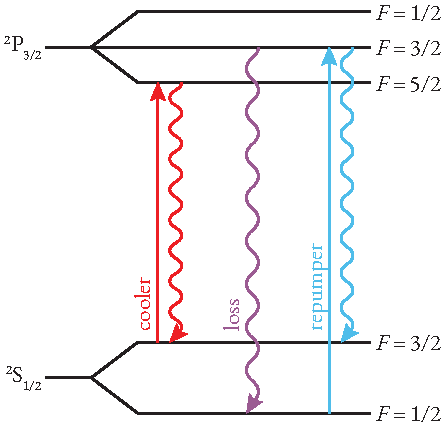
\includegraphics[]{\imagepath/cooler_repumper_in_alkali/cooler_repumper_in_alkali.pdf}
    \caption{Schematic of the cooling and repumping scheme in an alkali atom, here exemplarily for fermionic $^6$Li atoms ($I = 1, J_\text{g} = \frac{1}{2}$): the cooling cycle is $\Ket{\frac{1}{2}, \frac{3}{2}} \rightarrow \Ket{\frac{3}{2}, \frac{5}{2}} \rightsquigarrow \Ket{\frac{1}{2}, \frac{3}{2}}$. Atoms are lost if, during cooling, they end up in the $\Ket{\frac{3}{2}, \frac{3}{2}}$ state and decay down into the $\Ket{\frac{1}{2}, \frac{1}{2}}$ state. The repumper then leads them back into the cooling cycle via $\Ket{\frac{1}{2}, \frac{1}{2}} \rightarrow \Ket{\frac{3}{2}, \frac{3}{2}} \rightsquigarrow \Ket{\frac{1}{2}, \frac{3}{2}}$. As the $^2\text{P}_{3/2}$ manifold is not resolved for the cooler transition, the loss decay happens very often, and the rates of cooling and repumping are on the same order of magnitude.}
    \label{fig:cooler_repumper_in_alkali}
\end{figure}
\todo{Check with other source}


\paragraph{Magneto-optical Traps with Lithium}\ref{ch:3d_mots_with_li}
3-dimensional magneto-optical traps for lithium usually operate on the D$_2$ line, i.e.~between the $^2\text{S}_{1/2}$ and $^2\text{P}_{3/2}$ manifolds, as in the implementation in the FermiQP demonstrator. Since the first implementation with lithium in the early 1990s \cite{kawanaka_decay_1993}, they have become a standard part of ultracold lithium experiments, namely for experiments with fermionic~\cite{duarte_all-optical_2011,omran_microscopic_2015} and bosonic~\cite{kawanaka_decay_1993,schunemann_magneto-optic_1998} lithium as well as for isotope mixtures \cite{mewes_simultaneous_1999, schreck_sympathetic_2001, hilker_laser_2012, kerkmann_novel_2019} and species mixtures~\cite{ladouceur_compact_2009,tiecke_high-flux_2009,chen_lithium-cesium_2021}.

For D$_2$ line traps for fermionic lithium, the energy splitting between the two ground state hyperfine manifolds $\KetSpaced{J=1/2, F=1/2}$ and $\KetSpaced{J=1/2, F=3/2}$ is \SI{228}{\mega\hertz}, which sets the difference in frequency for the cooler and repumper laser beams. The cooler addresses the transition $\Ket{^2\text{S}_{1/2}, F = 3/2} \rightarrow \Ket{^2\text{P}_{3/2}}$, the repumper addresses the transition $\Ket{^2\text{S}_{1/2}, F = 1/2} \rightarrow \Ket{^2\text{P}_{3/2}}$. These transitions are shown in figure~\ref{fig:lithium_level_diagram}.

It is important to note that the hyperfine levels $F = \frac{5}{2}$, $\frac{3}{2}$, and $\frac{1}{2}$ of the excited state cannot be resolved because the D$_2$ line is broader than the splitting between these hyperfine states. This implies that it cannot be controlled which hyperfine state the cooler excites the atoms into. A large fraction of them will hence drop into the $\KetSpaced{J=1/2, F=1/2}$ state and need to be repumped. For this reason, the cooler and repumper have equal importance in a Lithium magneto-optical trap. Another implication is that coincidental sub-Doppler cooling, as observed in magneto-optical traps for other atomic species, cannot be expected to support the cooling process~\cite{grier_lambda-enhanced_2013}.

Typical parameter ranges for 3-dimensional traps with lithium from earlier experiments are~\cite{
    tiecke_high-flux_2009,
    kawanaka_decay_1993,
    schunemann_magneto-optic_1998,
    mewes_simultaneous_1999,
    hilker_laser_2012,
    kerkmann_novel_2019,
    ladouceur_compact_2009,
    chen_lithium-cesium_2021,    
    burchianti_efficient_2014,
    li_enhanced_2015,
}:
\begin{itemize}
    \item laser intensities: from a few up to more than ten saturation intensities, with a little less power on the repumper
    \item beam diameter: \SI{5}{\milli\meter} to \SI{15}{\milli\meter}
    \item detuning: mostly around $-5\Gamma$, up to $-8 \Gamma$ (\cite{li_enhanced_2015}), with the repumper often being less detuned than the cooler \todo{find a more realistic range}
    \item magnetic gradients: \SI{10}{\gauss\per\centi\meter} to \SI{50}{\gauss\per\centi\meter}
    \item achieved temperature: on the order of \SI{1e-3}{\kelvin} to \SI{3e-4}{\kelvin}
    \item atom number: around \SI{1e7}{} to \SI{1e8}{}
\end{itemize}

Lower temperatures than in magneto-optical traps operating on the D$_2$ line have been reached by using a UV transition~\cite{duarte_all-optical_2011,omran_microscopic_2015} which, however, requires expensive laser sources optical components~\cite{burchianti_efficient_2014}. More efficient loading rates have been achieved in a magneto-optical traps by adding sidebands onto the cooling light in order to address more velocity classes~\cite{li_enhanced_2015}.


\begin{figure}
    \centering
    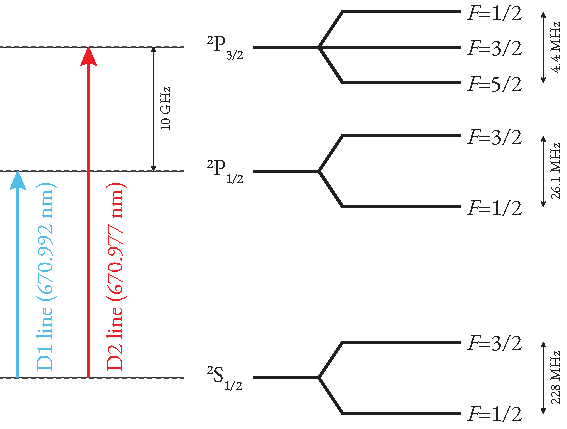
\includegraphics[]{\imagepath/lithium_level_diagram/lithium_level_diagram.pdf}
    \caption{Level diagram of fermionic lithium ($^6$Li) \cite{gehm_properties_2003, scherf_re-measurement_1996}: The transition between the  $^2\text{S}_{1/2}$ and the $^2\text{P}_{1/2}$ manifolds is called D$_1$ line with a frequency of $\SI{670.992}{\mega\hertz}$. The transition between the  $^2\text{S}_{1/2}$ and the $^2\text{P}_{3/2}$ manifolds is called D$_2$ line with a frequency of $\SI{670.977}{\mega\hertz}$. Both have a linewidth of $\Gamma = \SI{5.87}{\mega\hertz}$ which means that the $^2\text{P}_{3/2}$ manifold cannot be resolved with D$_2$ light. The hyperfine splitting in the $^2\text{S}_{1/2}$ manifold is \SI{228}{\mega\hertz}.}
    \label{fig:lithium_level_diagram}
\end{figure}

\subsection*{Gray Molasses Cooling}
The subsequent step in the cooling cycle in the FermiQP demonstrator, after the 3-dimensional magneto-optical trap, will be gray molasses cooling~\cite{grynberg_proposal_1994,weidemuller_novel_1994}. This sub-Doppler cooling technique operates on the D$_1$ line of lithium, i.e. the $^2\text{S}_{1/2} \rightarrow {^2\text{P}_{1/2}}$ transition~\cite{burchianti_efficient_2014}.

Gray molasses is based on atoms moving in a polarization-gradient field where they move up a potential hill until they decay into a lower energy state, similar to Sisyphus cooling~\cite{foot_atomic_2005}. Gray molasses operates on $\Delta J = 0$ transitions, as is the case for the D$_1$ line. This transition functions as a $\Lambda$ system with the two ground states being the states $\Ket{\text{ground}, m}$ and $\Ket{\text{ground}, m + 2}$ and the excited state being $\Ket{\text{excited}, m + 1}$~\cite{weidemuller_novel_1994}, as illustrated in figure~\ref{fig:gray_molasses_level_diagram}. Coupling between these states is polarization-dependent due to dipole selection rules.
\begin{figure}
    \centering
    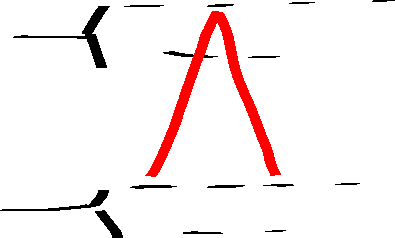
\includegraphics{\imagepath/gray_molasses_level_diagram/gray_molasses_level_diagram.pdf}
    \caption{$\Lambda$-system used in gray molasses cooling: It consists of two manifolds with equal $J$, connecting the two magnetic sublevels $m$ and $m+2$ in the ground state via $m+1$ in the excited state.}
    \label{fig:gray_molasses_level_diagram}
\end{figure}

The counter-propagating gray molasses beam have perpendicular polarization, e.g. circular polarization with different helicity. At every point the superposition of the polarization states of both beam yields an effective polarization sensed by the atoms. This effective polarization depends on the phase of the two light beams with respect of each other, that means that the atoms see alternating circular, elliptical, linear, elliptical, etc.~polarization along their journey through the light field. This makes the coupling between the relevant states position-dependent, as hinted at in figure~\ref{fig:gray_molasses_polarization_gradient}.

\begin{figure}
    \centering
    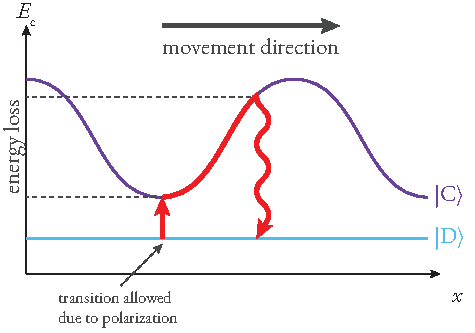
\includegraphics{\imagepath/gray_molasses_polarization_gradient/gray_molasses_polarization_gradient.pdf}
    \caption{Polarization-gradient in the gray molasses scheme: Atoms move along the light field and see different energy shifts $E_c$ depending on their position. At positions with low light shift, the polarization allows that they transition from the dark state $\Ket{\text{D}}$ to the coupling state $\Ket{\text{C}}$ and move further in the light field losing kinetic energy until they decay back.}
    \label{fig:gray_molasses_polarization_gradient}
\end{figure}

In the gray molasses' light field, the $\Lambda$-system is dressed with two orthogonal, hence not mutually coupling, eigenstates $\Ket{\text{C}}$ and $\Ket{\text{D}}$, being superpositions of the two ground states. One of them, $\Ket{\text{C}}$, couples to the light field via the excited state and experiences an energy shift $E_C \propto \frac{\Omega_\text{eff}^2}{\delta}$. The other, $\Ket{\text{D}}$, is a dark state~\cite{weidemuller_novel_1994,gerken_gray_2016}.

The absence of coupling between these two states only persists as long as the atoms' kinetic energy is not considered. For atoms with momentum $p$, there is a non-zero transition probability $P \propto \left|\frac{p}{E_C} \right|^2$~\cite{weidemuller_novel_1994}. This means that faster atoms are more prone to transition from the dark state to the coupling state, and that this transition is most likely in areas with low light intensity.

The cooling effect in this scheme can now be understood as follows: Atoms move along the gray molasses light field with a finite velocity $v$. At points with low light intensity, due to the polarization gradient, they are likely to transition from the dark state $\Ket{\text{D}}$ to the coupling state $\Ket{\text{C}}$. Moving further in the polarization-gradient field, their light shift energy $E_C$ increases, at the cost of their kinetic energy. When they spontaneously decay back into the dark state $\Ket{\text{D}}$ they lose an amount of energy on the order of the light shift $E_C$. This is illustrated in figure~\ref{fig:gray_molasses_polarization_gradient}. The gray molasses light needs to be blue detuned, $\delta > 0$, because then the light shift is positive, and the atoms lose energy falling back into the dark state $\Ket{\text{D}}$. With this scheme,  temperatures even below the recoil limit $T_\text{recoil}$ can be reached~\cite{weidemuller_novel_1994,gerken_gray_2016}.


\paragraph{Gray Molasses with Lithium} The D$_1$ line of lithium is just \SI{10}{\giga\hertz} off the D$_2$ line. This avoids the need for separate laser system in a different wavelength regime and  enables reusing optics of the magneto-optical trap for the gray molasses. Similar to the magneto-optical trap, a cooler and a repumper are needed: the former is blue detuned with respect to the $\Ket{^2\text{S}_{1/2}, F = 3/2} \rightarrow \Ket{^2\text{P}_{1/2}, F = 3/2}$ transition, the latter is blue detuned with respect to the $\Ket{^2\text{S}_{1/2}, F = 1/2} \rightarrow \Ket{^2\text{P}_{1/2}, F = 3/2}$. In contrast to cooling on the D$_2$ line, the excited manifold of the D$_1$ line is resolved, meaning the splitting between its excited state's hyperfine level is larger than its line width~\cite{gerken_gray_2016}.

\citeauthor{burchianti_efficient_2014} implemented gray molasses for fermionic lithium in 2014. Their parameters were taken as a reference starting point for configuring the gray molasses of the FermiQP demonstrator setup~\cite{burchianti_efficient_2014}:
\begin{itemize}
    \item laser intensities: $s_{0, \text{cooler}} = 2.7$, $\frac{I_\text{repumper}}{I_\text{cooler}} \approx 0.2$
    \item detunings: $\delta_\text{cooler} = +5.4 \Gamma$, varying $\delta_\text{repumper}$ between $(\delta_\text{cooler} -2 \Gamma)$ and  $(\delta_\text{cooler}+ 3\Gamma)$
\end{itemize}
with $I_s = \SI{7.59}{\milli\watt\per\square\centi\meter}$ and $\Gamma = \SI{5.8724}{\mega\hertz}$ for the D$_1$ line~\cite{gehm_properties_2003}.

\todo{Add transition to concrete implementation}

\section{Geometry}
The 3-dimensional magneto-optical trap of the FermiQP demonstrator is loaded from the atomic beam originating from the 2-dimensional magneto-optical trap. It is guided through a differential pumping stage separating the high and the ultra-high vacuum regions of the experiment chamber. The trap is located in the front part of the glass cell. The space around the glass cell is tightly packed with the two microscope objectives sitting above and below the trap and the Feshbach coils placed left and right of the incoming atomic beam, as shown in figure~\ref{fig:glass_cell_vicinity}. As a reminder, the reference coordinate system of the experiment chamber is that $x$ is along the atomic beam, $y$ is to the left as seen in the direction of the atomic beam, and $z$ is in upward direction.

\begin{figure}
    \centering
    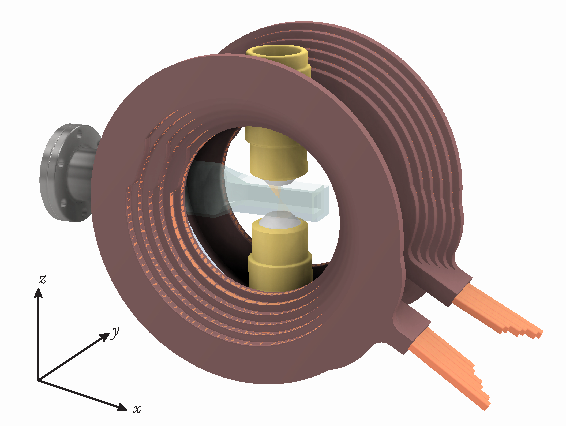
\includegraphics{\imagepath/glass_cell_vicinity/glass_cell_vicinity.pdf}
    \caption{Position of the glass cell between the microscope objectives and the Feshbach coils. The tightly packed vicinity of the glass cell determines the geometry of the magneto-optical trap.}\label{fig:glass_cell_vicinity}
\end{figure}

The magneto-optical trap needs three pairs of beams, one for each spatial degree of freedom that the atoms should be cooled along. For each pair, a beam is shot in from one side and retroreflected after passing through the glass cell. Due to the tightly packed vicinity of the glass cell, the beam axes cannot match with the Cartesian coordinate axes: no beams can be shot along the $z$ axis which is blocked by the objectives, and no beam can be shot directly along the atomic beam axis ($x$) because no retroreflection would be possible on the other side of the glass cell.

Instead, two beams are shone in in the $xz$ plane at an angle with respect to the atomic beam. The geometry of the microscope objectives only permits shooting beams into the glass cell at shallow angles, namely with an incidence angle of \SI{60}{\degree} with respect to the surface normal of the glass cell, as depicted in figure~\ref{fig:glass_cell_sides_mot_beams_0}. These beams provide cooling and confinement along the atomic beam axis ($x$, with an angle $\theta = \SI{30}{\degree}$ between light propagation $\vec k$ and velocity $\vec v$ of the atomic beam) and the up-down axis ($y$). The third beam is shot in along the $y$ axis, i.e.\ from left to right (see figure~\ref{fig:glass_cell_sides_mot_beams_1}). The beams are reflected back on reflection stages behind the glass cell.
\todo{name all beams consistently $y$ axis beam, (shallow) $xz$ axis beams}

\begin{figure}
    \centering
    \begin{subfigure}[t]{0.7\textwidth}
        \centering
        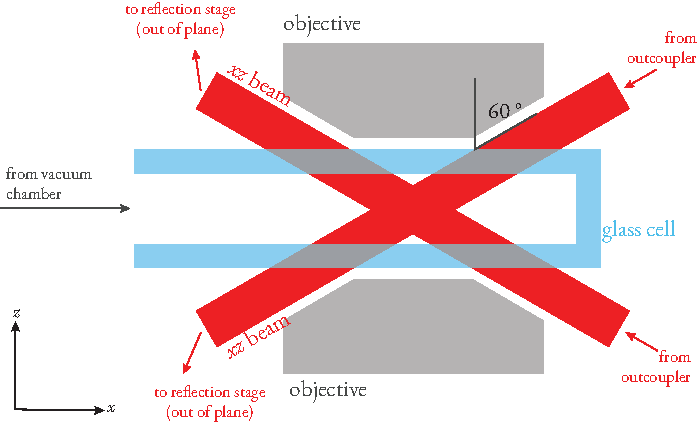
\includegraphics[scale=0.7]{\imagepath/glass_cell_sides_mot_beams/glass_cell_sides_mot_beams_1.pdf}
        \caption{$xz$ beams, view perpendicular to the atomic beam}\label{fig:glass_cell_sides_mot_beams_0}
    \end{subfigure}
    \begin{subfigure}[t]{0.29\textwidth}
        \centering
        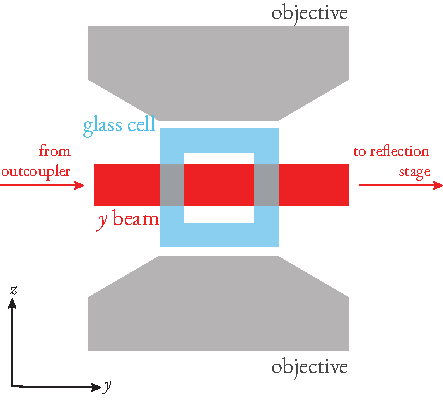
\includegraphics[scale=0.7]{\imagepath/glass_cell_sides_mot_beams/glass_cell_sides_mot_beams_0.pdf}
        \caption{The $y$ beam, view against the atomic beam}\label{fig:glass_cell_sides_mot_beams_1}
    \end{subfigure}
    \caption{Schematic side views of the glass cell and the trap beams: The $y$ beam comes in from the left/right. The two $xz$ beams come in under shallow angles, with incidence angles of \SI{60}{\degree} with respect to the glass cell surface normal. Behind the glass cell, the $xz$ beams are deflected away to their respective reflection stages. The beams have a diameter of \SI{7}{\milli\meter}. The glass cell has a side length of \SI{20}{\milli\meter} and \SI{4}{\milli\meter}-thick walls. Dimensions are to scale in this schematic. The change of the incidence angle of the $xz$ beams within the glass due to refraction was neglected in this schematic.}
    \label{fig:glass_cell_sides_mot_beams}
\end{figure} 

\section{Preparation of the Trap Laser Light}
The cooling laser beams for the 2-dimensional and the 3-dimensional magneto-optical traps as well as for the gray molasses are jointly produced on an optics board from where they are transferred to the experiment chamber via optical fibers.

The laser beams originate from two laser sources, one for D$_2$ light for the magneto-optical traps and one for D$_1$ light for the gray molasses. All beams produced by the setup consist of cooler and repumper light, which is separated by \SI{228}{\mega\hertz}, the hyperfine splitting of the $^2\text{S}_{1/2}$ ground state. For the 2-dimensional magneto-optical trap, the frequencies of the cooler and repumper light as well as their powers are fixed, for the 3-dimensional trap and the gray molasses light they need to be variable in order to compress and optimize the traps dynamically. The light for the 3-dimensional trap and the gray molasses cooling should be prepared on the same optical path, which is useful as both cooling schemes are carried out at the same position in the experiment chamber. All beams need to have sufficient power levels such that several saturation intensities on the respective trap cross-sections (\SI{30}{\milli\meter} for the 2-dimensional trap and \SI{7}{\milli\meter} for the 3-dimensional trap and the gray molasses cooling).\todo{Give exemplary power levels for realistic saturation intensities. Finish sentence.}

\subsection*{Laser sources}
The \SI{671}{\nano\meter} laser light for the D$_2$ and D$_1$ lines is jointly produced for all aforementioned cooling beams by two Raman fiber amplifiers (MPB VRFA-P-1500-671-SF-PLUS, \textit{Socrates} and \textit{Plato}) with a specified output power of \SI{1.5}{\watt} each. They are supplied with seed light by two single-mode diode lasers at \SI{1342}{\nano\meter} (Toptica MDL pro, \textit{Heraklitus} seeding \textit{Socrates}, and \textit{Zeno} seeding \textit{Plato}), delivering around \SI{20}{\milli\watt} of power. Each fiber amplifier contains a frequency-doubling stage creating a \SI{671}{\nano\meter} laser beam of \SI{1}{\milli\meter} diameter from the amplified \SI{1342}{\nano\meter} light. The seed lasers are offset-locked to a global reference laser that itself is locked to an ultra-low expansion cavity. The offset locking allows shifting the laser frequencies of the D$_2$ and the D$_1$ light arbitrarily within a range of a few hundred \si{\mega\hertz} \todo{verify}. The interplay of these lasers is outlined in figure~\ref{fig:laser_interplay_schematic}.

\begin{figure}
    \caption{Schematic of the cooling laser setup: Two Raman fiber amplifiers provide light for the optics setups that prepare the light used in the magneto-optical traps and the gray molasses. The amplifiers are offset-locked via their seeds to a global reference lasers which, in turn, is locked to a reference cavity.
    \todo[inline]{add image}
    }\label{fig:laser_interplay_schematic}
\end{figure}


The main advantage of using the Raman fiber amplifiers is that they produce enough optical power to simultaneously supply all three aforementioned traps with light. An alternative would be separate laser sources, each of which would need to be frequency-locked and monitored independently. During the writing of the thesis, the Raman fiber amplifiers showed signs of substantial degradation as their output power decreased by over \SI{20}{\percent} in only a few weeks of intermittent operation. The details and the severity of this degradation are presented in~\cite{qesja_design_2022}. As the experimenters of FermiQP, as well as the manufacturers, could not come up with a quick and reliable solution to this problem that could be verified during the writing of this thesis, it stays uncertain whether the Raman fiber amplifiers can be used long-term for the laser cooling within the FermiQP demonstrator. An alternative approach would be amplification of the seed light using tapered amplifier chips.

\subsection*{Important Optical Elements}
The following optical components were among the main building blocks of the optics setup that is described in the following:
\begin{itemize}
    \item Polarizing beam splitter cube (PBS): Polarizing beam splitter cubes spatially split a laser beam into its $\KetText{H}$- and $\KetText{V}$-polarized components. The $\KetText{H}$ component passes through the cube while the $\KetText{V}$ component is deflected. In the setup described below, polarizing beam splitter cubes are used for splitting a laser beam into portions of arbitrary power using a preceding half-wave plate for setting the incident polarization accordingly, and for overlapping two beams of different polarization into a common spatial mode. The polarizing beam splitter cubes used for building the laser setup were manufactured by CeNing optics with a specified transmission extinction ratio error of $\frac{1}{1000}$ and a surface reflectivity of $<\SI{0.25}{\percent}$.
    \item Wave plate: Wave plates allow changing the polarization of a beam. Wave plates are made of birefringent crystals cut to the right length such that the there is a defined phase retardation between the fast and the slow axis of the crystal. Half-wave plates generate a \SI{180}{\degree} phase difference, quarter-wave plates generate a \SI{90}{\degree} phase difference between their axes. Depending on the angle between the axes of the crystal and the polarization components of the beam, half-wave plates can turn linear polarization into any other arbitrary linear polarization, whereas quarter-wave plates introduce ellipticity in the polarization and hence can generate circularly polarized light. Using a quarter- and a half-wave plate, linear polarization can be turned into any arbitrary polarization state. For turning an arbitrary polarization state into any other polarization state, an arrangement of quarter-, half-, and another quarter-wave plate is necessary as a single quarter-wave plate cannot arbitrarily change the ellipticity of incident elliptical light.\footnote{An intuitive example of why only a quarter- and a half-wave plate are not sufficient for turning an arbitrary polarization state into any other polarization state is the transformation of circular light into elliptical light of any arbitrary ellipticity: A quarter-wave plate always transforms circularly polarized light into linearly polarized light, so at least another quarter-wave plate is necessary for creating arbitrary ellipticity.} The wave plates used for building the laser setup were zero-order wave plates sold by Laser Components (part numbers:  WPZ-671-04-2-R05, WPZ-671-09-2-R10, WPZ-671-04-4-R05,  WPZ-671-09-4-R10) with a specified retardance threshold of $\frac{\lambda}{300}$ and reflectance of $<\SI{0.2}{\percent}$.
    \item Acousto-optic modulator (AOM): Acousto-optic modulators allow changing the optical frequency of a laser beam by multiples of the operating frequency $f_\text{AOM}$. The beam is sent through a crystal in which the index of refraction $n$ is spatially modulated perpendicular to the beam direction by an acoustic wave of frequency $f_\text{AOM}$. The incident laser light is diffracted on this spatial modulation of the index of refraction, leading to multiple light beams after of the modulator at angles $\theta_m$ with $\sin \theta_m = m\frac{\lambda_\text{light}}{\lambda_\text{acoustic}}$ where $m \in \{..., -2, -1, 0, 1, 2, ...\}$ is the order of each refracted beam and $\lambda_\text{light}, \lambda_\text{acoustic}$ are the optical and acoustic wave lengths. A beam of order $m$ is frequency-shifted by $\Delta f = mf_\text{AOM}$~\cite{hunsperger_acousto-optic_2002}. In the optical setup described below, acousto-optic modulators are used for increasing or decreasing the frequency of a laser beam and as fast optical shutters by switching the diffraction on and off. Sending light forwards and backwards through an acousto-optic modulator using a mirror, a so-called double pass, doubles the frequency shift of the light and avoids the angular diffraction, which cancels out for both passes through the modulator. While propagating through the double pass, the light is polarization-turned from $\KetText{H}$ to $\KetText{V}$ using a quarter-wave plate passed in forward and backward direction such that incoming and outgoing beams can be separated on a polarizing beam splitter. Typical coupling efficiencies for the first order are \SIrange[]{80}{90}{\percent}. The acousto-optic modulators used for building the laser setup were produced by Gooch \& Housego (part numbers: 3080-120, frequency range: \SI{80(10)}{\mega\hertz}, active aperture of \SI{1}{\milli\meter} and 3110-120, frequency range: \SI{110(12)}{\mega\hertz}, active aperture of \SI{0.6}{\milli\meter}).
    \item Telescope: A telescope reduces the diameter of a collimated laser beam. It consists of two lenses, the first being convex ($f > 0$) focusing down the laser beam, the second being concave ($f < 0$) for re-collimating the beam.
    \item Incoupler: An incoupler arrangement feeds a free-space laser beam into an optical fiber. The beam is focused down onto the tip of the fiber using an aspheric lens with an appropriate focal length such that the waist of the focused beam matches with the fiber size.
    \item Mirror: \todo{add mirrors with specs and info about LC mirrors polarization checks}
\end{itemize}

\subsection*{Outline of the Laser Setup}
The necessary output beams for the traps and the gray molasses are created from the two input beams on the D$_2$ and the D$_1$ frequency as depicted in figure~\ref{fig:laser_setup_schematic}.



\begin{figure}
    \centering
    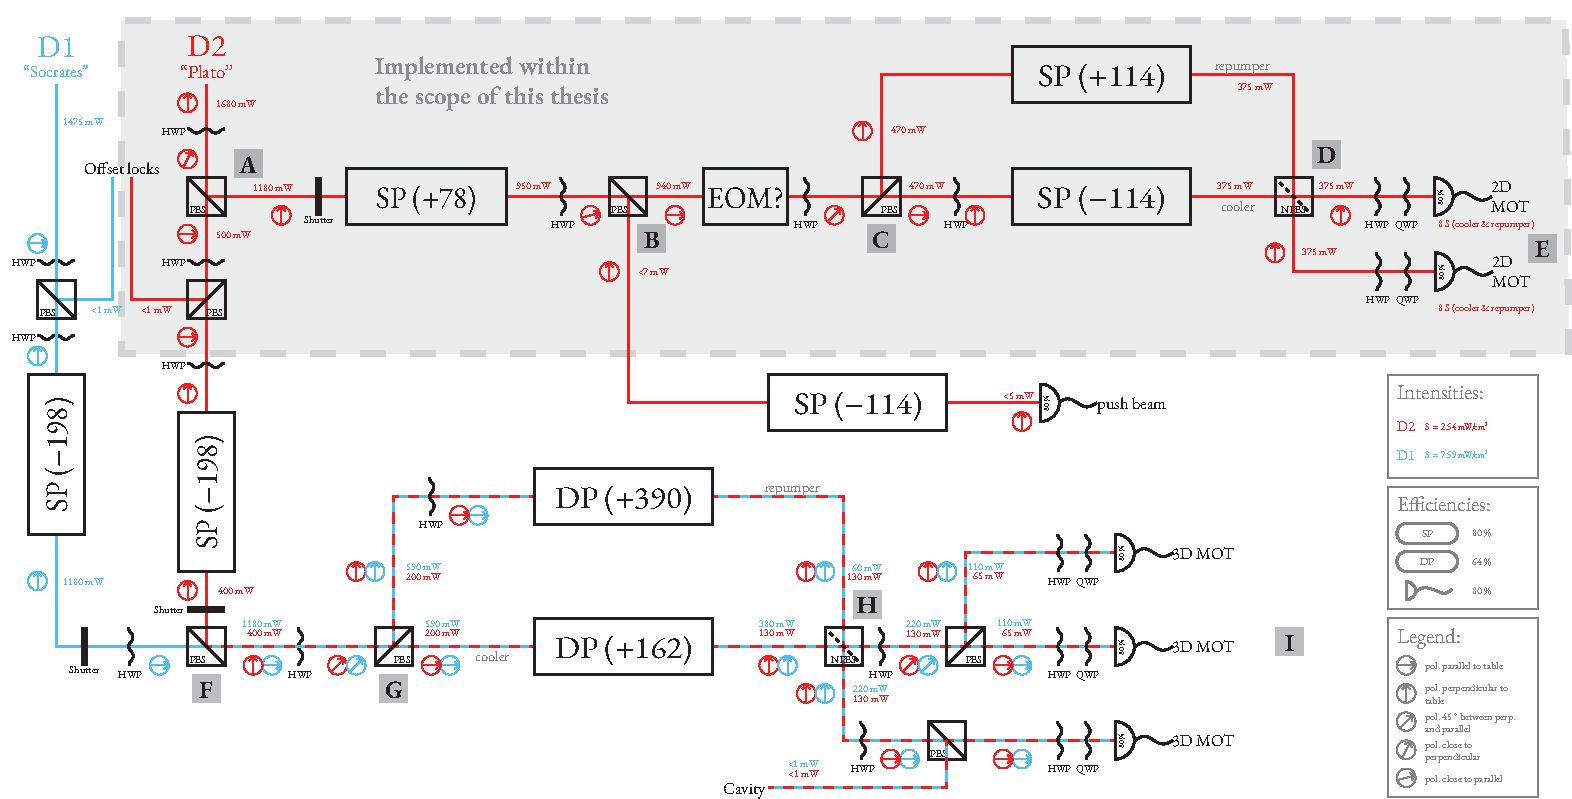
\includegraphics[width=\textwidth]{\imagepath/laser_setup_schematic/laser_setup_schematic.pdf}
    \caption{Schematic of the laser setup for preparing the cooling light for the magneto-optical traps and the gray molasses: D$_2$ light is split into two branches for the 2-dimensional (to the right) and the 3-dimensional magneto-optical (to the bottom) traps at the first PBS (A).
    For the light for the 2-dimensional trap, a small amount of power is taken out for the push beam (B) before it is split into cooler and repumper (C) light for the two outputs. It is considered to add an electro-optical modulator for improving the cooling effect of the light. This part of the laser setup was constructed within the scope of this thesis.
    The light for the 3-dimensional trap and the D$_1$ light for the gray molasses are spatially overlapped (D), split into cooler and repumper (E), and then distributed into three outputs (F).
    SP and DP boxes stand for single pass and double pass acousto-optic modulators respectively, the number denotes the applied frequency in \si{\mega\hertz}.
    \todo[inline]{TODO update image: remove unnecessary details, remove saturation intensities, add 2D-MOT board boundary, add letter markers, add RFA names, add EOM}}
    \label{fig:laser_setup_schematic}
\end{figure}

The D$_2$ light is offset-locked \SI{-78}{\mega\hertz} below the actual D$_2$ transition frequency. It is split into on a polarizing beam splitter into a path for the 2-dimensional and one for the 3-dimensional magneto-optical trap. The power splitting ratio was preliminarily set to about $\frac{1}{3}$ for the 3-dimensional and $\frac{2}{3}$ for the 2-dimensional optical trap since the 2-dimensional trap needs to reach the required intensity for a larger trap cross-section, and it is the first cooling stage of the experiment bridging the large range from several hundred Kelvin to sub-Kelvin temperatures on two of three spatial axes.

\paragraph{2d Trap Branch} The branch for the 2-dimensional trap can be blocked using a shutter and an acousto-optic modulator used as a fast optical switch steered by the experiment control system. The shutter is a loudspeaker magnet with a beam blocker attached to it and acts as an additional slow controllable beam blockade ensuring that definitely no light can pass. This acousto-optic modulator increases the laser frequency by \SI{+78}{\mega\hertz} such that the light is resonant with the D$_2$ transition again. Using another half-wave plate and beam splitter, a small fraction of the laser power is branched off for the push beam. This light is frequency-shifted by \SI{+114}{\mega\hertz} in order to be resonant with the cooler transition. The remaining light is used in the trap.

The experimenters consider adding an electro-optical modulator at this point for improving the trap. This modulator would add frequency sidebands at \si{\mega\hertz} to the light. In the trap, these additional frequencies would address other velocity classes than the original light and might hence increase the loading rate of the trap.

After that the light is split in a power ratio of approximately $1$:$1$ into cooler and repumper beams, each of which is fed through an acousto-optic modulator with driving frequencies of \SI{-114}{\mega\hertz} and \SI{+114}{\mega\hertz} for cooler and repumper respectively, which corresponds to the hyperfine splitting of the ground state manifold. When the magneto-optical traps are implemented, the frequency splitting between cooler and repumper might be experimentally optimized for maximize fluorescence of the 2-dimensional and loading rate of the 3-dimensional magneto-optical trap. The two beams are then spatially overlapped on a beam splitter and fed to two optical fibers leading to the experiment chamber.

\paragraph{3d Trap Branch} From the branch of the D$_2$ light for the 3-dimensional trap, a small amount is branched off for offset-locking. The remaining light is sent through a modulator-shutter combination for programmatic beam blocking as explained above, here with a modulator frequency of \SI{-198}{\mega\hertz}. It is then spatially overlapped with the D$_1$ light. The D$_1$ light is also offset by \SI{+78}{\mega\hertz}, a part of it split off for offset locking, and fed through an identical programmatic beam blockade. The combined beam of D$_2$ and D$_1$ light is then also split into two paths for cooler and repumper in a ratio of approximately $1$:$1$. Here, however, the light is fed through acousto-optic modulator double-passes as described in~\cite{qesja_design_2022}. As the net deflection is zero in double passes, it allows a programmatic change of the frequency shift applied to each beam without the need to realign optical components. Together with the ability to damp the laser power by reducing the modulators' radio-frequency driving power, frequency and power of each beam can be independently steered for compressing the 3-dimensional magneto-optical trap and for switching the powers when applying the gray molasses. The cooler beam is frequency shifted by about \SI{+162}{\mega\hertz}, the repumper by about \SI{+390}{\mega\hertz}, with the double-passes allowing for an adjustment range of several tens of \si{\mega\hertz}. The total frequency shift considering the initial offset, the blockade modulators and modulator in the cooler (repumper) path amounts to $\SI{-78}{\mega\hertz} - \SI{198}{\mega\hertz} + \SI{390}{\mega\hertz} = \SI{+114}{\mega\hertz}$ ($\SI{-78}{\mega\hertz} - \SI{198}{\mega\hertz} + \SI{162}{\mega\hertz} = \SI{-114}{\mega\hertz}$) which is again the hyperfine splitting of the ground state manifold.\todo{add paragraphs}

\subsection*{Implementation of the Laser Setup for the 2-dimensional Magneto-optical Trap}
Within this thesis, the part of the laser setup providing the light for the 2-dimensional magneto-optical trap, as highlighted in figure~\ref{fig:laser_setup_schematic}, was built.
Important optical components used and the implementation of the optics board is described in greater detail in this paragraph, figure~\ref{fig:2d_mot_setup_photo} shows a photograph of this part of the setup.

\begin{figure}
    \centering
    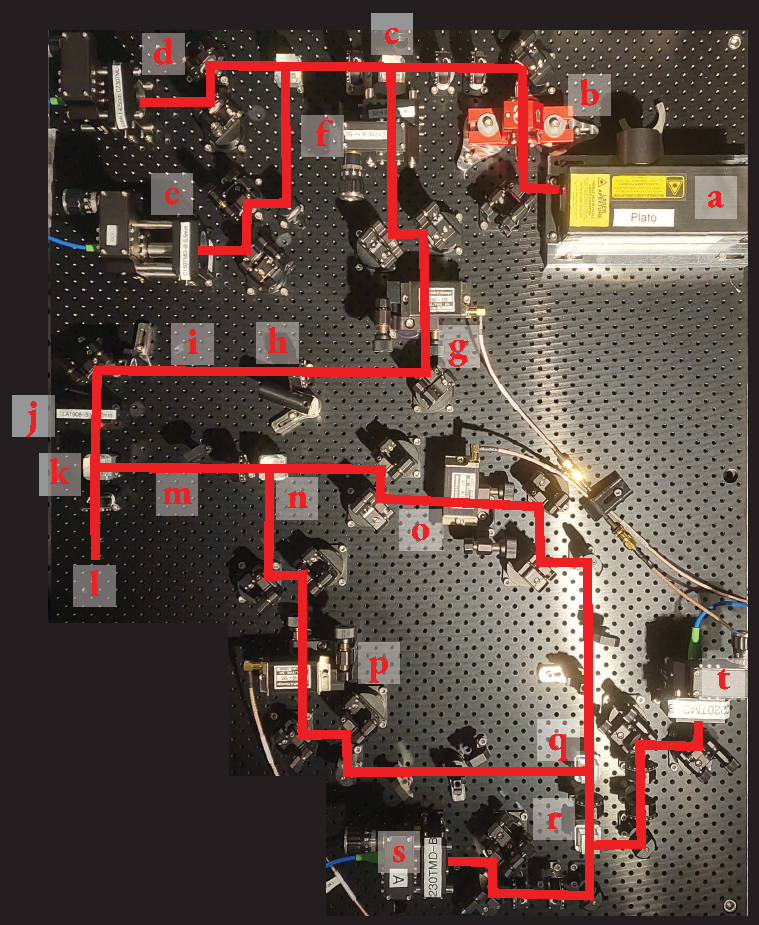
\includegraphics[width=\textwidth]{\imagepath/2d_mot_setup_photo/2d_mot_setup_photo.pdf}
    \caption{Photograph of the part of the optics setup providing light for the 2-dimensional magneto-optical trap. The beam path and reference points have been added for orientation.}\label{fig:2d_mot_setup_photo}
\end{figure}

The light is prepared on the optics board in the following steps (letters reference points in figure~\ref{fig:2d_mot_setup_photo}):
\begin{itemize}
    \item[a] The D$_2$ light is coming from the doubling stage of the Raman fiber amplifier ``Plato'' where the amplified \SI{1342}{\nano\meter} light is frequency-doubled to \SI{671}{\nano\meter} light. At this point, the laser beam has a $\frac{1}{\text{e}^2}$ diameter of about \SI{1000}{\micro\meter}.

    \item[b] In order to prevent any inadvertent reflections travelling back into the amplifier, a Newport optical isolator (Newport ISO-04-650-MP-WP) was placed immediately after the doubling stage. In a power measurement, \SI{30}{\deci\bel} damping (with the isolator inverted) and \SI{95}{\percent} transmission could be attested in agreement with the specifications.

    \item[c] After the optical isolator, a quarter-wave plate is used to eliminate any elliptical polarization components from the beam caused by hitting mirrors with light that has polarization other than $\Ket{\text{H}}$ and $\Ket{\text{V}}$.

    \item[d] The D$_2$ light is split into the paths for the different magneto-optical traps with a half-wave plate and a polarizing beam splitter. All other polarizing beam splitters in the same setup are of the same model and specifications. The splitting ratio between the beams was not yet fixed during the course of this thesis.

    \item[e, f] The light transmitted on this beam splitter is again split and coupled into optical fibers leading to the offset lock (f) and to the other optics board hosting the rest of the setup (e, for details see~\cite{qesja_design_2022}). The light reflected off on the beam splitter is used for the push beam and the 2-dimensional magneto-optical trap.

    \item[g] As the acousto-optic modulators used in the setup require way smaller beam diameters than the \SI{1000}{\micro\meter} beam output by the Raman fiber amplifier, a telescope for decreasing the beam diameter was placed after the aforementioned beam splitter cube. The telescope consists of a convex lens ($f = \SI{75}{\milli\meter}$) focusing the beam and a concave lens ($f = \SI{-50}{\milli\meter}$) re-collimating it after about \SI{30}{\milli\meter}. This reduces the beam diameter to about \SI{650}{\micro\meter} immediately after the second lens, the beam waist is now about $2w_0 = \SI{600}{\micro\meter}$ located about \SI{175}{\milli\meter} away from the telescope. Lowering the beam diameter is a trade-off between a slimmer beam waist $w_0$ making the beam fitting better into the acousto-optic modulators' apertures and a larger beam divergence $\theta = \frac{\lambda}{\pi w_0}$ that would lead to even larger beam diameters after some propagation distance. The scaled-down beam reaches a diameter of about \SI{700}{\micro\meter} after about \SI{475}{\milli\meter} after the telescope. In order to scale it down for the rest of the beam path on the board, a convex lens ($f = \SI{500}{\milli\meter}$) was placed in the beam path. In this way, the beam diameter is kept under \SI{700}{\micro\meter} on the remaining beam path with the waist (diameter $2w_0 \approx \SI{650}{\micro\meter}$) at a total distance of \SI{720}{\milli\meter} from the telescope.  These parameters were estimated based on a simulation in the software GaussianBeam~\cite{noauthor_gaussianbeam_nodate}, shown in figure~\ref{fig:beam_diameter_evolution}.

\begin{figure}
    \caption{Evolution of the beam shape from the telescope along the beam path
    \todo[inline]{add image}
    }
    \label{fig:beam_diameter_evolution}
\end{figure}

    \item[h] The slimmed-down light is then coupled through the first acousto-optic modulator operated at \SI{+78}{\mega\hertz}. The zeroth order of the outgoing beam is blocked at i. The power efficiency of this acousto-optic modulator single pass is \SI{83}{\percent} (see also table~\ref{tab:power_loss_table}). Thanks to the telescope, the beam diameter at this point is significantly smaller than the specified aperture.
    
    \item[i] A half-wave plate sets the splitting ratio between light for the push beam (m) and light for the 2-dimensional magneto-optical trap.
    
    \item[j] At this position the shutter will be placed in order to be able to completely bar any light from entering the magneto-optical trap.
    
    \item[k] Here the light is refocused using an $f = \SI{500}{\milli\meter}$ lens as described for point g. This sizes down the beam diameter such that it doesn't exceed the aperture of the acousto-optic modulators for creating the cooler and repumper beams (p, q).
    
    \item[l] The light is split into a few \si{\milli\watt} for the push beam (m) and the rest for the 2-dimensional magneto-optical trap.

    \item[m] Here the push beam light will be prepared using a single pass acousto-optic modulator driven at \SI{+114}{\mega\hertz} which serves as a frequency shifter and as a shutter.
    
    \item[n] At this point, space is left free for an electro-optical modulator that would add sidebands onto the light allowing for addressing more velocity classes in the trap and thus increasing its loading rate.
    
    \item[o] With a half-wave plate and a polarizing beam splitter, the light is split into cooler (q) and repumper (p) paths. The polarizations of the beams are $\KetText{V}$ of the cooler and $\KetText{H}$ of the repumper beam.
    
    \item[p, q] The cooler (q) and repumper (p) paths each contain an acousto-optic modulator operated at \SI{+114}{\mega\hertz} and \SI{-114}{\mega\hertz} respectively. Thanks to the refocusing lens (k), the beam diameter approximately matches the modulators' apertures. The power efficienies are \SI{76}{\percent} for the cooler and \SI{81}{\percent} for the repumper (see also table~\ref{tab:power_loss_table}).
    
    \item[r, s] The cooler and repumper beam are spatially overlapped in split into two paths on a combination of two polarizing beam splitter cubes and a half-wave plate. Due to their polarizations, the cooler is reflected on the first cube (r) while the repumper passes through it, both leaving the cube on the same port. A half-wave plate then turns their respective polarizations to diagonal $\KetText{D}$ and anti-diagonal $\KetText{A}$. A subsequent polarizing beam splitter cube (s) splits both cooler and repumper into two equally strong beams.
    
    \item[t, u] The two resulting beams are coupled into fibers guiding it to the experiment chamber. In each beam, a pair of a quarter- and half-wave plate allow for arbitrary corrections of the polarization if necessary. The coupling efficiencies after the assembly of the optics board are \SI{84}{\percent} for fiber A (t) and \SI{74}{\percent} for fiber B (u) for both cooler and repumper (see also table~\ref{tab:power_loss_table}). When the magneto-optical traps are implemented and the frequencies of the cooler and repumper beams are optimized, the light needs to be coupled into the two fibers from anew as the deflection angles on the respective acousto-optic modulators will also change.
\end{itemize}

Table \ref{tab:power_table} lists measured remaining power levels after each dissipating element (tab.~\ref{tab:power_loss_table}) as well as measured recombination (tab.~\ref{tab:power_recombination}) and splitting ratios (tab.~\ref{tab:power_splitting}).

\begin{table}
    \centering
    \begin{subtable}{\textwidth}
        \centering
        \begin{tabular}{lllc}
            \toprule
            \multicolumn{2}{l}{\textbf{element}} & \textbf{markers} (fig.~\ref{fig:2d_mot_setup_photo}) & \textbf{power after element} \\
            \toprule
            isolator & & a - d & \SI{97}{\percent} \\
            \midrule
            telescope & & g - h & \SI{99}{\percent} \\
            \midrule
            \multirow{3}{*}{switching AOM} & all orders & h & \SI{100}{\percent} \\ 
            & positive orders & h - k & \SI{89}{\percent} \\
            & first order & h - o & \SI{83}{\percent} \\
            \midrule
            \multirow{2}{*}{cooler AOM} & all orders & q & \SI{97}{\percent} \\
            & first order  & q - r & \SI{76}{\percent} \\
            \midrule
            \multirow{2}{*}{repumper AOM} & all orders & p & \SI{99}{\percent} \\
            & first order  & p - r & \SI{81}{\percent} \\
            \midrule
            \multirow{3}{*}{fiber A} & cooler \& repumper & s - t & \SI{84}{\percent} \\
            & cooler & q - t & \SI{78}{\percent} \\
            & repumper & p - t & \SI{81}{\percent} \\
            \midrule
            \multirow{3}{*}{fiber B} & cooler \& repumper & s - u & \SI{74}{\percent} \\
            & cooler & q - u & \SI{71}{\percent} \\
            & repumper & p - u & \SI{77}{\percent} \\
            \bottomrule
        \end{tabular}
        \caption{Measured remaining powers after dissipating elements}
        \label{tab:power_loss_table}
    \end{subtable}

    \vspace{1cm}
    \begin{subtable}{0.5\textwidth}
        \centering
        \begin{tabular}{llc}
            \toprule
            \textbf{beam} & \textbf{markers} (fig.~\ref{fig:2d_mot_setup_photo}) & \textbf{percentage} \\
            \toprule
            cooler & q - r & \SI{51}{\percent} \\
            repumper & p - r & \SI{47}{\percent} \\
            \bottomrule
        \end{tabular}
        \caption{Measured power ratios of the recombined cooler and repumper beams on the polarizing beam splitter cube r}
        \label{tab:power_recombination}
    \end{subtable}

    \vspace{1cm}
    \begin{subtable}{0.65\textwidth}
        \centering
        \begin{tabular}{lllc}
            \toprule
            \textbf{beam} & \textbf{branch} & \textbf{markers} (fig.~\ref{fig:2d_mot_setup_photo}) & \textbf{ratio} \\
            \toprule
            \multirow{2}{*}{cooler \& repumper} & A & s - t & \SI{50}{\percent} \\
            & B & s - u & \SI{51}{\percent} \\
            \midrule
            \multirow{2}{*}{cooler} & A & q - t & \SI{49}{\percent} \\
            & B & q - u & \SI{53}{\percent} \\
            \midrule
            \multirow{2}{*}{repumper} & A & p - t & \SI{51}{\percent} \\
            & B & p - u & \SI{49}{\percent} \\
            \bottomrule
        \end{tabular}
        \caption{Measured power splitting ratios into branches A and B on the polarizing beam splitter cube s}
        \label{tab:power_splitting}
    \end{subtable}
    
    \caption{Measured power dissipations and power ratios on the optics board for the 2-dimensional magneto-optical trap}
    \label{tab:power_table}
\end{table} 


\section{Projected Implementation}
In this section, the projected trap implementation is outlined. The geometry of the trapping beams with respect to the glass cell is explained. The planned optical setup around the experiment chamber is outlined, as well as how it needs to be configured to create the necessary polarization in the trap. Some estimations on the light intensities and magnetic gradients are given. The section concludes with a forecast about the properties of the trap.

\subsection*{Optics around the Experiment Chamber}
The six cooling laser beams for the 3-dimensional magneto-optical trap are transferred from the optics board to the experiment chamber with optical fibers. 

One trap beam will be shot in along the $y$ axis,  thus from the left or right side of glass cell, and will be reflected back directly on a reflection stage at the other side of the glass cell. The two other beams, the $xz$ beams, are shot into the glass cell from the upper and lower front of the glass cell through the upper sides at an angle of \SI{60}{\degree} with respect to glass surface in order not to be blocked by the microscope objectives (as explained in the geometry section above, see figure~\ref{fig:glass_cell_sides_mot_beams}). For reflecting these beams back into the glass cell, they are first guided away from the experiment chamber onto stand-alone reflection stages as there wouldn't be enough space for these stages between the experiment chamber and the glass cell (see figure~\ref{fig:mot_optics_schematic_from_above}).

\begin{figure}
    \centering
    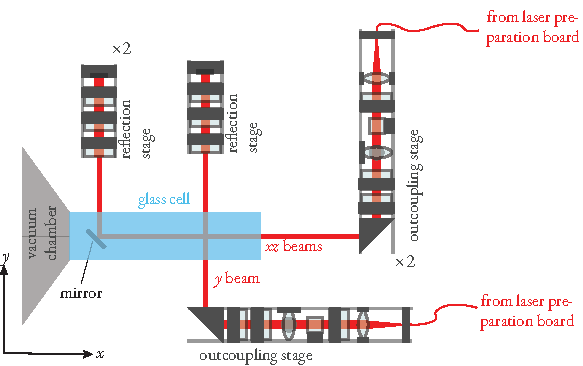
\includegraphics[]{\imagepath/mot_optics_schematic_from_above/mot_optics_schematic_from_above.pdf}
    \caption{Schematic of the optics for the 3-dimensional magneto-optical trap from above: The reflection stages of the $xz$ beams would not fit between the glass cell and the vacuum chamber. Instead, the $xz$ beams are reflected away from the chamber on a mirror onto the $xz$ reflection stages farther away from the chamber.
    \todo[inline]{replace stages by miniature copies of the stage schematics}
    }
    \label{fig:mot_optics_schematic_from_above}
\end{figure}

\paragraph{Outcoupling Stages}
The outcoupling stages consist of optical elements for collimating, polarization-cleaning, and polarization-preparing the light, mounted in an optical cage system. A schematic of the stage is shown in figure~\ref{fig:outcoupling_stage_schematic}

\begin{figure}
    \centering
    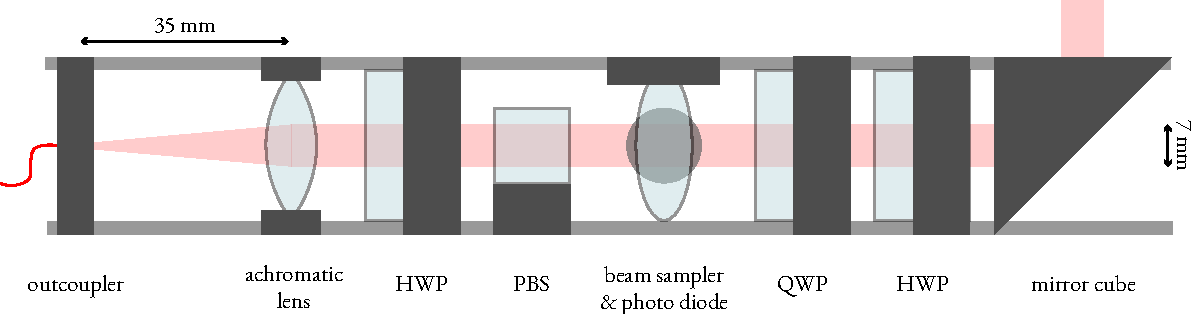
\includegraphics[width=\textwidth]{\imagepath/outcoupling_stage_schematic/outcoupling_stage_schematic.pdf}
    \caption{Schematic of the outcoupling stage in an optical cage system: The trapping light coming from an optical fiber is collimated with an achromatic lens with a focal length of \SI{35}{\milli\meter} such that the beam has a $\frac{1}{e^2}$ diameter of \SI{7}{\milli\meter}. The polarization is cleaned using a half-wave plate and a polarizations beam splitter. Using a beam sampler, a small amount of light is reflected out of the axis and shot onto a photodiode for power monitoring. The light is polarization-prepared on a quarter- and a half-wave plate.}
    \label{fig:outcoupling_stage_schematic}
\end{figure}

The light leaving the optical fiber has a divergence angle of $\theta = \frac{\lambda}{\pi w} = \frac{\SI{671}{\nano\meter}}{\pi\SI{2.25}{\micro\meter}} = \SI{95}{\milli\radian}$ with the beam waist $w = \SI{2.25}{\micro\meter}$ at the fiber tip. In order to collimate it to a beam of $\frac{1}{e^2}$ diameter of \SI{7}{\milli\meter}, hence radius of $r_{1/e^2} = \SI{3.5}{\milli\meter}$, a lens of focal length $f = \frac{r_{1/e^2}}{\tan \theta} = \frac{\SI{3.5}{\milli\meter}}{\SI{95}{\milli\radian}} \approx \SI{35}{\milli\meter}$~\cite{noauthor_collimated_2021} is installed in the outcoupling stage such that the fiber tip is in the focal point.

In order to clean the polarization that the light might have acquired while travelling in the fiber, is cleaned using a combination of a half-wave plate and a polarizing beam splitter.

After that a beam sampler reflects out a small fraction of the light onto a photodiode for power monitoring. Note that the power is monitored after polarization cleaning in order to check the effective power that is available for trapping\footnote{The power is not monitored on the other beam splitter port as then one could not distinguish between polarization-induced and supply-induced power changes. It is also not checked by monitoring the transmitted power on one of the system's mirrors as the absolute power transmitted through these mirrors would be too little.}.

Finally, the polarization of the trapping beam can be set using a quarter- and a half-wave plate.

\paragraph{Reflection Stages}
The reflection stages consist of an cascade of a quarter-, a half-, and another quarter-wave plate and a mirror mounted in a cage system, as depicted in figure~\ref{fig:reflection_stage_schematic}. This threefold wave plate combination is traversed by the light twice, forwards and backwards, and allows for arbitrary changes of polarization. Only using two wave plates in the reflection stage would not suffice as a combination of only one quarter- and one half-wave plate cannot map every polarization to any other arbitrary polarization.

\begin{figure}
    \centering
    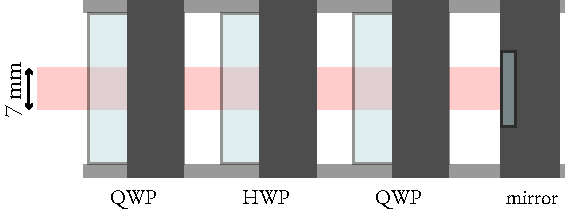
\includegraphics[scale=0.77]{\imagepath/reflection_stage_schematic/reflection_stage_schematic.pdf}
    \caption{Schematic of the reflection stage in an optical cage system: Incoming light is sent through a quarter-, a half-, and anther quarter-wave plate, and then reflected on a mirror. It leaves the stage propagating through the three wave plates again in reverse order.}
    \label{fig:reflection_stage_schematic}
\end{figure}

\subsection*{Polarization}
The trapping light needs to have circular polarization at the trap position in the glass cell, either with left or right helicity for both the forward and the backward pass, depending on the direction of the magnetic gradient. Since the polarization cannot be measured within the glass cell at the time of operation, the approximate configuration of the optics for attaining the necessary polarization is estimated.

In the following, the Jones vector notation for polarization in the horizontal-vertical basis $\{\KetText{H}, \KetText{V}\}$ is going to be used to denote the circular polarization states $\KetText{R}$ and $\KetText{L}$ and the diagonal polarization states $\KetText{D}$ and $\KetText{A}$:
\begin{align}
        \text{circular:} && \KetText{R} &= \frac{1}{\sqrt{2}} \left(\KetText{H} - i \KetText{V}\right),  & \KetText{L} &= \frac{1}{\sqrt{2}} \left(\KetText{H} + i \KetText{V}\right) \\
        \text{diagonal:} && \KetText{D} &= \frac{1}{\sqrt{2}} \left(\KetText{H} + \KetText{V}\right),  &  \KetText{A} &= \frac{1}{\sqrt{2}} \left(\KetText{H} - \KetText{V}\right)
\end{align}
Here, horizontal polarization $\KetText{H}$ is defined as parallel to the glass cell surface  where the beam enters the cell, vertical polarization $\KetText{V}$ is perpendicular to $\KetText{H}$. For the $y$ beams, $\KetText{V}$ is also parallel to the glass cell surface. For the $xz$ beams, $\KetText{V}$ encloses a \SI{30}{\degree} angle with the surface normal of the glass cell surface.

For the $y$ axis trap beam entering the glass cell from the left or right, the circular polarization can directly be set on the wave plates in the outcoupling stage. As the light enters the glass cell perpendicular to its surface, the polarization will not be affected when transmitted through the glass.

For the other two $xz$ beams entering at shallow angles with $\theta = \SI{60}{\degree}$ between the surface normal and the beam, the difference in transmission coefficients for $\KetText{H}$ and $\KetText{V}$ polarization components needs to be considered and the wave plates on the outcoupling and the reflection stages must be set accordingly.

The glass cell is made of fused silica with a refractive index of $n = \SI{1.456}{}$ at \SI{671}{\nano\meter} \cite{malitson_interspecimen_1965}. According to Snell's law, for the $xz$ beams the angle between the light and the surface normal in the glass is $\theta_\text{glass} = \arcsin \frac{\sin \theta}{n} = \SI{36.5}{\degree}$~\cite{demtroder_elektromagnetische_2013}. The transmission coefficients for the two polarization components are then~\cite{demtroder_elektromagnetische_2013}
\begin{align}\label{eq:fresnel}
    \begin{split}
        t_{\KetText{H}, \text{air} \rightarrow \text{glass}}(\theta, \theta_\text{glass})  &= \frac{2 \cos \theta}{\cos \theta + n \cos \theta_\text{glass}}\\
        t_{\KetText{H}, \text{glass} \rightarrow \text{air}}(\theta, \theta_\text{glass})  &= \frac{2n \cos \theta_\text{glass}}{n \cos \theta_\text{glass} + \cos \theta} \\
        t_{\KetText{V}, \text{air} \rightarrow \text{glass}}(\theta, \theta_\text{glass})  &= \frac{2 \cos \theta}{n \cos \theta + \cos \theta_\text{glass}}\\ 
        t_{\KetText{V}, \text{glass} \rightarrow \text{air}}(\theta, \theta_\text{glass})  &= \frac{2 n \cos \theta_\text{glass}}{\cos \theta_\text{glass} + \cos \theta}\\ 
    \end{split}
\end{align}
where the $\text{s}$ and $\text{p}$ components of the polarization have been mapped to the $\KetText{H}$ and $\KetText{V}$ basis vectors respectively. For the $y$ beam, they evaluate to $t_{\text{air} \rightarrow \text{glass}}(\SI{0}{\degree}, \SI{0}{\degree}) = \SI{0.814}{}$, $t_{\text{glass} \rightarrow \text{air}}(\SI{0}{\degree}, \SI{0}{\degree}) = \SI{1.186}{}$.\footnote{Note that it is not unphysical if $t > 0$. The transmitted power on a surface from air to a material with $n > 1$ is $\frac{n \cos \theta_\text{transmitted}}{\cos \theta_\text{incident}}t^2$ which is always less than $1$~\cite{demtroder_elektromagnetische_2013}.} For the $xz$ beams, they evaluate to $t_{\KetText{H}, \text{air} \rightarrow \text{glass}}(\theta, \theta_\text{glass}) = t_{\KetText{H}, \text{glass} \rightarrow \text{air}}(\theta, \theta_\text{glass}) = \SI{0.916}{}$, $t_{\KetText{V}, \text{air} \rightarrow \text{glass}}(\theta, \theta_\text{glass}) = t_{\KetText{V}, \text{glass} \rightarrow \text{air}}(\theta, \theta_\text{glass}) = \SI{0.999}{}$.
\todo{Check values and propagate if they were wrong}

The total transmission coefficient through the \SI{4}{\milli\meter}-thick wall of the glass is combined transmission into glass and back into air:
\begin{align}
    t_{y} &= t_{\KetText{H}, \text{air} \rightarrow \text{glass}}(\SI{0}{\degree}, \SI{0}{\degree})  \cdot t_{\KetText{H}, \text{glass} \rightarrow \text{air}}(\SI{0}{\degree}, \SI{0}{\degree}) = \SI{0.965}{} \\
    \begin{split}
        t_{xz, \KetText{H}} &= t_{\KetText{H}, \text{air} \rightarrow \text{glass}}(\theta, \theta_\text{glass})  \cdot t_{\KetText{H}, \text{glass} \rightarrow \text{air}}(\theta, \theta_\text{glass}) = \SI{0.839}{} \\
        t_{xz, \KetText{V}} &= t_{\KetText{V}, \text{air} \rightarrow \text{glass}}(\theta, \theta_\text{glass})  \cdot t_{\KetText{V}, \text{glass} \rightarrow \text{air}}(\theta, \theta_\text{glass}) = \SI{0.998}{}
    \end{split}
\end{align}

\paragraph{First pass}
In order to attain circular polarization on the first pass through the glass cell, these polarization-dependent losses need to be pre-compensated when choosing the polarization before the glass cell surface:
\begin{align}
    \label{eq:predicted_polarizations_first_pass}
    \Ket{\psi_{\text{before cell,} {\text{right} \atop \text{left}}}} 
    = \frac{1}{\sqrt{\frac{1}{t_{\KetText{H}}^2} + \frac{1}{t_{\KetText{V}}^2}}}
        \left(\frac{\KetText{H}}{t_{\KetText{H}}} \mp i \frac{\KetText{V}}{t_{\KetText{V}}} \right)
    = 0.765 \KetText{H} \mp 0.644i \KetText{V}
\end{align}

\begin{figure}
    \centering
    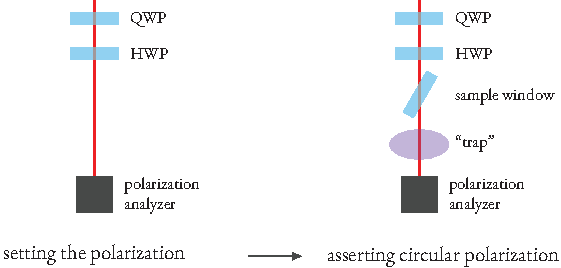
\includegraphics[]{\imagepath/first_pass_polarization_measurement_scheme/first_pass_polarization_measurement_scheme.pdf}
    \caption{Schematic of the experimental setup for verifying the polarization of the incident trapping light for the first pass through the glass cell: At first, the predicted polarizations (equations~\eqref{eq:predicted_polarizations_first_pass}) were set and verified using a polarization analyzer. Then a sample glass plate was put in and circular polarization after the plate (the ``trap'' position) was asserted.}
    \label{fig:first_pass_polarization_measurement_scheme}
\end{figure}

For verifying these polarizations in a mock setup, a sample fused silica glass plate of thickness \SI{4.04}{\milli\meter} was placed at an angle of \SI{60}{\degree} with respect to a \SI{671}{\nano\meter} laser beam. This glass plate acts as the surface through which the light enters the glass cell. Using a quarter- and a half-wave plate, the polarization before the plate could be arbitrarily set by monitoring it on a polarization analyzer. Then the glass plate was put into the beam path and and circular polarization was asserted after the glass plate, as outlined in figure~\ref{fig:first_pass_polarization_measurement_scheme}. The results are displayed in table~\ref{tab:polarization_first_pass} and show that the aforementioned estimated polarizations  are a good estimate for producing circular polarization in the glass cell.

\begin{table}
    \centering

    \begin{tabular}{ccc}
        \toprule
        \textbf{target polarization} & \textbf{set before glass plate} & \textbf{measured after glass plate} \\
        \toprule
        $\KetText{R}$ & $0.78 \KetText{H} + (-0.02-0.63i) \KetText{V}$ & $0.70 \KetText{H} +(0.00-0.71i)\KetText{V}$ \\
        $\KetText{L}$ & $0.75 \KetText{H} + (-0.01+0.67i)\KetText{V}$ & $0.70 \KetText{H} + (0.00+0.71i)\KetText{V}$ \\
        \bottomrule
    \end{tabular}
    \caption{Results of the experimental verification of the preset polarization for the first pass through the glass cell, as outlined in figure~\ref{fig:first_pass_polarization_measurement_scheme}. The measured polarizations after the glass plate confirm that the proposed pre-compensation~\eqref{eq:predicted_polarizations_first_pass} is a good estimate. All values are outputs of the polarization analyzer, transformed from the azimuth-ellpticity basis to the Jones basis as described in the appendix chapter~\ref{ch:pypol_trafos}.}
        \label{tab:polarization_first_pass}
\end{table}

\paragraph{Second pass}\todo{explain why we need three waveplates more in depth mentioning all important properties}
In order to attain the same circular polarization on the second pass through the glass cell, the wave plates on the reflection stages must be set accordingly. Their required configuration is determined experimentally since the glass surfaces and mirrors in the beam path introduce many polarization changes that are hard to deduct from principle. Again, a mock setup with a sample glass plate with a shallow angle with respect to the beam is used. This time, it acts as the surface which the light leaves the glass cell through.

Light is transmitted through a polarizing beam splitter cube, then circularly polarized using a quarter-wave plate. This light mimics the trap light before leaving the glass cell on the first pass. It is then transmitted through the sample glass plate at the shallow angle of \SI{60}{\degree}, simulating the exit from the glass cell. Afterwards the light is deflected onto a mock reflection stage, made up of a quarter-, a half-, and another quarter-wave plate, and finally onto a mirror sending the light back through the setup such that it reaches the beam splitter cube again. This arrangement is outlined in figure~\ref{fig:second_pass_waveplate_adjustment_scheme}. For the mirrors used for deflecting the beam onto the reflection stage (Laser Componenets \todo{model name and specs}), it was verified that individual mirrors all change the polarization in the same way at an incidence angle of \SI{45}{\degree}.

The ideal wave plate configuration on the reflection stage is now identified by monitoring the power reflected on the polarizing beam splitter depending on the wave plate configuration: Light passing back through the setup with the same circular polarization as on the first pass will be completely transmitted back through the beam splitter cube after traversing the quarter-wave plate in reverse direction. This means that for the desired configuration, all light of the second pass will be transmitted on the beam splitter cube, and the deflected power on the cube is minimal.

The complete evolution of polarization in the setup is for right polarization in the cell
\begin{align}
    \label{eq:second_pass_waveplate_adjustment_cascade_r}
    \underset{\substack{\text{beam}\\\text{splitter}}}{\longrightarrow}
    \KetText{H} 
    \underset{\substack{\text{quarter}\\\text{wave plate}}}{\longrightarrow}
    \KetText{R}
    \underset{\substack{\text{mirror \&}\\\text{wave plates}}}{\longrightarrow}
    \Ket{\psi_\text{R}}
    \underset{\substack{\text{mirror}}}{\longrightarrow}
    M\Ket{\psi_\text{R}}
    \underset{\substack{\text{wave plates \&}\\\text{mirror}}}{\longrightarrow}
    \KetText{R}
    \underset{\substack{\text{quarter}\\\text{wave plate}}}{\longrightarrow}
    \KetText{H}
    \underset{\substack{\text{beam splitter}\\\text{port 1}}}{\longrightarrow}
\end{align}
and for left polarization in the cell
\begin{align}
    \label{eq:second_pass_waveplate_adjustment_cascade_l}
    \underset{\substack{\text{beam}\\\text{splitter}}}{\longrightarrow}
    \KetText{H} 
    \underset{\substack{\text{quarter}\\\text{wave plate}}}{\longrightarrow}
    \KetText{L}
    \underset{\substack{\text{mirror \&}\\\text{wave plates}}}{\longrightarrow}
    \Ket{\psi_\text{L}}
    \underset{\substack{\text{mirror}}}{\longrightarrow}
    M\Ket{\psi_\text{L}}
    \underset{\substack{\text{wave plates \&}\\\text{mirror}}}{\longrightarrow}
    \KetText{L}
    \underset{\substack{\text{quarter}\\\text{wave plate}}}{\longrightarrow}
    \KetText{H}
    \underset{\substack{\text{beam splitter}\\\text{port 1}}}{\longrightarrow}
\end{align}
with the polarization flip $M = \left(\begin{smallmatrix}1&0\\0&-1\end{smallmatrix}\right)$ caused by a mirror. The polarizations $\Ket{\psi_\text{R}}$ and $\Ket{\psi_\text{L}}$ identify the ideal wave plate configuration and are hence the observed parameter looked for in the mock setup. $\Ket{\psi_\text{R}}$ and $\Ket{\psi_\text{L}}$ can be measured by replacing the mirror with the polarization analyzer after an optical wave plate configuration has been found, as outlined in figure~\ref{fig:second_pass_waveplate_adjustment_scheme}.

The ideal polarizations were identified by finding the minima of light power on port 2 of the beam splitter ($< \SI{1}{\percent}$ of the power after the sample window). They are listed in table~\ref{tab:polarization_second_pass}.

\begin{figure}
    \centering
    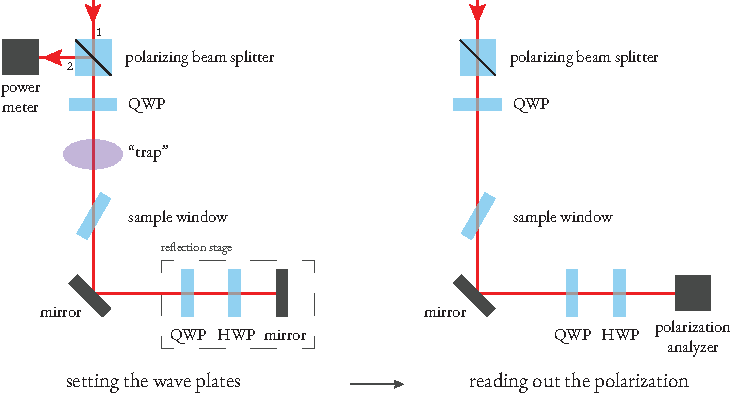
\includegraphics[]{\imagepath/second_pass_waveplate_adjustment_scheme/second_pass_waveplate_adjustment_scheme.pdf}
    \caption{Schematic of the experimental setup for finding the right configuration of the wave plates on the reflection stages: In a first step, the wave plate configuration on the "reflection stage" is optimized for circular polarization in the ``trap'' by maximizing the output power on port 2 of the beam splitter cube. Then the polarization in the reflection stage which identifies the optimal waveplate configuration is measured using a polarization analyzer.}\label{fig:second_pass_waveplate_adjustment_scheme}
\end{figure}

\begin{table}
    \centering
    \begin{tabular}{cl}
        \toprule
        \textbf{target polarization $P$} & \textbf{polarization $\Ket{\psi_P}$ in reflection stage} \\
        \toprule
        $\KetText{R}$ & $0.71 \KetText{H} + (0.70+0.09i) \KetText{V}$ \\
        $\KetText{L}$ & $0.62\KetText{H} + (0.77+0.17i)\KetText{V}$ \\
        \bottomrule
    \end{tabular}
    \caption{Experimentally found ideal polarizations after the first pass through the reflection stage. For these polarizations, the light is circularly polarized on the backward pass through the mock setup (see figure~\ref{fig:second_pass_waveplate_adjustment_scheme}). All values are outputs of the polarization analyzer, transformed from the azimuth-ellipticity basis to the Jones basis as described in the appendix chapter~\ref{ch:pypol_trafos}.}
    \label{tab:polarization_second_pass}
\end{table}

When building the trap, the polarization presets for the first and the second pass through the glass cell (tables~\ref{tab:polarization_first_pass} and ~\ref{tab:polarization_second_pass}) should be deemed an initialization point for getting a first signal. The trap then needs to be optimized by varying the polarization configuration and monitoring its loading rate with fluorescence imaging.

\subsection*{Intensity}
The intensity of the trapping light is reduced along the optical path by the reflections on the glass surfaces and scattering by the atoms in the trap. In the following, $T_{1 \rightarrow 2}(\theta_1, \theta_2) = \frac{n_2 \cos \theta_2 }{n_1 \cos \theta_2} t_{1\rightarrow 2}^2$ denotes the power transmitted on a surface from medium $1$ to medium $2$ with beam angle $\theta_i$ in medium $i$ and a transmission coefficient of $t$~\cite{demtroder_elektromagnetische_2013}.

In the first pass, the intensity loss is due to reflections on the two surfaces of the glass cell wall. For the $y$ axis beam that hits the glass cell perpendicular to its surface, and the remaining relative power is determined by the transmission coefficient at \SI{0}{\degree} (equations ~\ref{eq:fresnel}). For the $xz$ axis beams (with polarization state $0.765 \KetText{H} \mp 0.644i \KetText{V}$, cf. equation~\ref{eq:predicted_polarizations_first_pass}), the remaining relative power is composed of the transmissions at an incidence angle $\theta = \SI{60}{\degree}$ for the two polarization components:
\begin{align}
    p_{y, \text{first pass}} = T_{y, \text{in}} &= T_{\text{air} \rightarrow \text{glass}}(\SI{0}{\degree}) T_{\text{glass} \rightarrow \text{air}}(\SI{0}{\degree}) = \left(\frac{1}{n} t^2_{\text{air} \rightarrow \text{glass}}(\SI{0}{\degree})\right) \left(n t^2_{\text{glass} \rightarrow \text{air}}(\SI{0}{\degree})\right) = \SI{0.932}{}\\
    \begin{split}
        p_{xz, \text{first pass}} = T_{xz, \text{in}} &= 0.765^2 T_{xz, \KetText{H}} + 0.644^2 T_{xz, \KetText{V}} \\
        &=  0.765^2 \left(\frac{1}{n} t^2_{\KetText{H}, \text{air} \rightarrow \text{glass}}(\theta)\right) \left(n t^2_{\KetText{H}, \text{glass} \rightarrow \text{air}}(\theta_\text{glass})\right) \\ &~~~~~+ 0.644^2 \left(\frac{1}{n} t^2_{\KetText{V}, \text{air} \rightarrow \text{glass}}(\theta)\right) \left(n t^2_{\KetText{V}, \text{glass} \rightarrow \text{air}}(\theta_\text{glass})\right) \\
        &= 0.765^2 \cdot (0.916^2 \cdot 0.999^2) + 0.644^2 \cdot (0.999^2 \cdot 0.916^2) = 0.837
    \end{split}
\end{align}

These values could be asserted by measuring optical power in a mock setup using a sample glass plate, similar to the ones for setting the polarization (figures~\ref{fig:first_pass_polarization_measurement_scheme} and~\ref{fig:second_pass_waveplate_adjustment_scheme}). The measured intensity losses are listed in table~\ref{tab:intensity_losses}.

In the second pass, the first loss $T_{\text{out}}$ is due to reflections on the two surfaces of the other glass cell wall upon exit from the glass cell. There, both beams have circular polarization before entering the glass:
\begin{align}
    T_{y, \text{out}} &= T_{y, \text{in}} = 0.932 \\
    T_{xz, \text{out}} &= \frac{1}{2} T_{xz, \KetText{H}} + \frac{1}{2} T_{xz, \KetText{V}} = 0.837
\end{align}
The second loss $T_{\text{in}}$ is due to entering the glass cell again with the same polarization as in the first pass. In addition, relative losses $1 - p_\text{scatter}$ from scattering in the first pass affect the beam power in the second pass. The remaining power in the second pass compared to the power in the first pass is
\begin{align}
    p_{y, \text{first pass} \rightarrow \text{second pass}} &= p_\text{scatter} \cdot T_{y, \text{out}} T_{y, \text{in}}   =  0.867 p_\text{scatter}\\
    p_{xz, \text{first pass} \rightarrow \text{second pass}} &= p_\text{scatter} \cdot T_{xz, \text{out}} T_{xz, \text{in}}   = 0.701 p_\text{scatter},
\end{align}
and the remaining power in the first pass compared to the original input power is
\begin{align}
    p_{y, \text{input} \rightarrow \text{second pass}} &= T_{y, \text{in}} \cdot p_\text{scatter} \cdot T_{y, \text{out}} T_{y, \text{in}} =  0.810 p_\text{scatter} \\
    p_{xz, \text{input} \rightarrow \text{second pass}} &= T_{xz, \text{in}} \cdot p_\text{scatter} \cdot T_{xz, \text{out}} T_{xz, \text{in}} = 0.586 p_\text{scatter},
\end{align}
$p_\text{scatter}$ depends on the geometry and density of the trapped atom cloud as well as the scattering rate, which in turn depends on the laser parameters.

Table~\ref{tab:intensity_losses} lists all of these relative intensity losses.

\begin{table}
    \centering
    \begin{tabular}{llc}
        \toprule
        & \textbf{predicted loss} & \textbf{measured loss} \\
        \toprule
        $p_{y, \text{first pass}}$ & \SI{93.2}{\percent} & \SI{94}{\percent} \\
        $p_{xz, \text{first pass}}$ & \SI{83.7}{\percent} & \SI{84}{\percent} \\
        \midrule
        $p_{y, \text{first pass} \rightarrow \text{second pass}}$ & $\SI{86.7}{\percent} \cdot p_\text{scatter}$ & \\
        $p_{xz, \text{first pass} \rightarrow \text{second pass}}$ & $\SI{70.1}{\percent} \cdot p_\text{scatter}$ & \\
        \midrule
        $p_{y, \text{input} \rightarrow \text{second pass}}$ & $\SI{81.0}{\percent} \cdot p_\text{scatter}$ & \\
        $p_{xz, \text{input} \rightarrow \text{second pass}}$ & $\SI{58.6}{\percent} \cdot p_\text{scatter}$ & \\
        \bottomrule
    \end{tabular}
    \caption{Remaining intensities on the first and the second pass through the glass cell surface for the $y$ and the $xz$ beams. First pass intensities were experimentally verified on a mock setup.}
    \label{tab:intensity_losses}
\end{table}

In order to achieve a similar cooling effect in both directions for each axis, meaning the first and second pass through the glass cell, the beam diameters $d$ could be reduced in the second pass with a focusing lens such that the intensities $I \propto \frac{1}{d^2}$ are equal in both passes,
\begin{align}\label{eq:intensity_focusing}
\frac{I_\text{second pass}}{I_\text{first pass}} =  \frac{T_\text{out} T_\text{in} p_\text{scatter} / d^2_\text{second pass}}{1/ d^2_\text{first pass}} = 1 ~~\Rightarrow~~ \frac{d_\text{second pass}}{d_\text{first pass}} = \sqrt[]{T_\text{out} T_\text{in} p_\text{scatter}}.
\end{align}

This would amount to $\left(\frac{d_\text{second pass}}{d_\text{first pass}}\right)_y = \SI[]{0.931}{} \cdot \sqrt{p_\text{scatter}}$ and $\left(\frac{d_\text{second pass}}{d_\text{first pass}}\right)_{xz} = \SI[]{0.837}{} \cdot \sqrt{p_\text{scatter}}$.


\subsection*{Magnetic Gradient}
The magnetic gradients for the 3-dimensional magneto-optical trap are produced by the Feshbach coils sitting positioned to the glass cell (see chapter~\ref{ch:coils}). Thanks to the high currents that are planned for for the Feshbach operation, the coils can generate high gradients upon reversal of the current in one of the coils. As elaborated in chapter~\ref{ch:field_characterization}, the achievable gradients in the trapping region are ideally \SI{99}{\gauss\per\centi\meter} in the $xz$ axis, where the recapturing axis lies, and even \SI{197}{\gauss\per\centi\meter} along the $y$ axis.



\subsection*{Trap Parameter Estimation}
In this section, the properties of the geometry, the trapping light and the magnetic gradients are used to estimate some basic quantities about the 3-dimensional magneto-optical trap.

\paragraph{Trap Dimensions}
As depicted in figure~\ref{fig:mot_extent}, the size of the trap as outlined by the $\frac{1}{e^2}$-diameter envelopes of the laser beams is \SI[]{14}{\milli\meter} in the recapturing direction (along $x$), \SI[]{8.1}{\milli\meter} along the $z$ axis, and extends over the whole glass cell in $y$ direction.

If the reflection losses on the glass cell surface are compensated for by focusing the beam as suggested in \eqref{eq:intensity_focusing}, the beam diameter and thus also the trap size would decrease to $\SI[]{11.7}{\milli\meter}$ in $x$ direction, and $\SI[]{6.8}{\milli\meter}$ in $z$ direction, assuming negligible losses from scattering ($p_\text{scatter} \approx 0$).

\begin{figure}
    \centering
    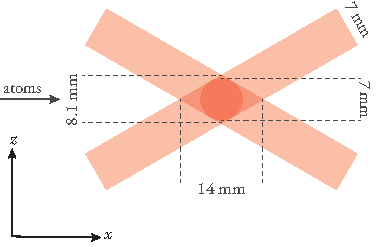
\includegraphics[]{\imagepath/mot_extent/mot_extent.pdf}
    \caption{Extent of the trap volume set by the $\frac{1}{e^2}$-diameters of the three trap laser beams: $2\cdot \SI[]{7}{\milli\meter} = \SI[]{14}{\milli\meter}$ in $x$ direction, unbounded in $y$ direction, and $\frac{\SI[]{7}{\milli\meter}}{\cos \SI[]{30}{\degree}} = \SI[]{8.1}{\milli\meter}$ in $z$ direction. If the intensity is kept constant on the second pass through the glass cell by focusing the beam, the beam diameters would be smaller by the factor of at least \SI{0.931}{} for the $y$ beam and \SI{0.837}{} for the $xz$ beams (see equation \ref{eq:intensity_focusing}).}
    \label{fig:mot_extent}
\end{figure}

In addition to that, the atoms recaptured from the atomic beam are subject to a maximum trapping radius depending on their velocity $v$ due to the resonance condition~\eqref{eq:resonance_radius}.

\paragraph{Intensity Estimation}
Assuming optical powers of about \SI{60}{\milli\watt} for each beam of the 3-dimensional magneto-optical trap (D$_2$ light), as estimated in figure~\ref{fig:laser_setup_schematic}, the average intensity in a beam for the magneto-optical trap would amount to $\frac{\SI{60}{\milli\watt}}{\pi (\SI{.35}{\centi\meter})^2} = \SI{156}{\milli\watt\per\centi\meter\squared}$ which amounts to a saturation of $s_0 = 31$ for cooler and repumper respectively. Along the recapturing axis ($x$), this leads to an effective saturation for the magneto-optical trap of
\begin{align}
    s_{0, \text{MOT, recapturing axis}} = 31 \cdot \cos \SI{30}{\degree} \cdot 2 = 53
\end{align}
where $\cos \SI{30}{\degree}$ originates from the shallow angles of incidence and the factor of $2$ accounts for the fact that both $xz$ beams cool along the recapturing axis. This saturation is large compared to the intensities reported for other trap implementations (cf. section~\ref{ch:3d_mots_with_li}) which means that there is a considerable power overhead for the 3-dimensional magneto-optical trap in the FermiQP demonstrator.

For the gray molasses, the average intensity of the D$_1$ light would be $\frac{\SI{90}{\milli\watt}}{\pi (\SI{0.35}{\centi\meter})^2} = \SI{247}{\milli\watt\per\centi\meter\squared}$ which would amount to $s_0 = 16$ for the cooler beam.

\paragraph{Capture and Resonance Velocities}
For a trap length of \SI[]{14}{\milli\meter} and saturation $s_0 \gg 1$, the maximum velocity for the small $^6$Li atoms recaptured from the atomic beam can be estimated with \eqref{eq:capture_velocity_high}:
\begin{align}
    v_\text{max, capture} = \sqrt{\frac{\hbar k \Gamma \cdot \SI[]{14}{\milli\meter}}{m}} = \SI[]{90}{\meter\per\second}
\end{align}

Note that this value is the maximum ideal value for atoms entering the trap exactly along the \SI{14}{\milli\meter}-long center line through the trapping light field. Atoms that are off this line will see a shorter trap radius and thus be constrained by a lesser capture velocity, let alone the diminished light intensity there.

The resonance velocity~\eqref{eq:resonance_velocity} tell which maximum velocity atoms can still have to be on resonance when entering the trap given a certain magnetic gradient and laser detuning $\delta_\text{laser} = \omega_\text{laser} - \omega_\text{transition}$. Atoms faster than that would require even further detuned light to be on resonance. The resonance velocity is mapped in figure~\ref{fig:resonance_velocity_map} outlining how  gradient and detuning can be traded for each other at a fixed resonance velocities. For $\delta_\text{laser} = -5\Gamma$, a gradient of \SI[]{57}{\gauss\per\centi\meter} would be required to reach $v_\text{max, resonance} \approx v_\text{max, capture}$.


\begin{figure}
    \centering
    \begin{pgfpicture}
        \pgftext{%% Creator: Matplotlib, PGF backend
%%
%% To include the figure in your LaTeX document, write
%%   \input{<filename>.pgf}
%%
%% Make sure the required packages are loaded in your preamble
%%   \usepackage{pgf}
%%
%% Also ensure that all the required font packages are loaded; for instance,
%% the lmodern package is sometimes necessary when using math font.
%%   \usepackage{lmodern}
%%
%% Figures using additional raster images can only be included by \input if
%% they are in the same directory as the main LaTeX file. For loading figures
%% from other directories you can use the `import` package
%%   \usepackage{import}
%%
%% and then include the figures with
%%   \import{<path to file>}{<filename>.pgf}
%%
%% Matplotlib used the following preamble
%%   \usepackage{fontspec}
%%   \setmainfont{DejaVuSerif.ttf}[Path=\detokenize{/home/max/.local/lib/python3.8/site-packages/matplotlib/mpl-data/fonts/ttf/}]
%%   \setsansfont{DejaVuSans.ttf}[Path=\detokenize{/home/max/.local/lib/python3.8/site-packages/matplotlib/mpl-data/fonts/ttf/}]
%%   \setmonofont{DejaVuSansMono.ttf}[Path=\detokenize{/home/max/.local/lib/python3.8/site-packages/matplotlib/mpl-data/fonts/ttf/}]
%%
\begingroup%
\makeatletter%
\begin{pgfpicture}%
\pgfpathrectangle{\pgfpointorigin}{\pgfqpoint{3.688881in}{2.462874in}}%
\pgfusepath{use as bounding box, clip}%
\begin{pgfscope}%
\pgfsetbuttcap%
\pgfsetmiterjoin%
\definecolor{currentfill}{rgb}{1.000000,1.000000,1.000000}%
\pgfsetfillcolor{currentfill}%
\pgfsetlinewidth{0.000000pt}%
\definecolor{currentstroke}{rgb}{1.000000,1.000000,1.000000}%
\pgfsetstrokecolor{currentstroke}%
\pgfsetdash{}{0pt}%
\pgfpathmoveto{\pgfqpoint{0.000000in}{0.000000in}}%
\pgfpathlineto{\pgfqpoint{3.688881in}{0.000000in}}%
\pgfpathlineto{\pgfqpoint{3.688881in}{2.462874in}}%
\pgfpathlineto{\pgfqpoint{0.000000in}{2.462874in}}%
\pgfpathlineto{\pgfqpoint{0.000000in}{0.000000in}}%
\pgfpathclose%
\pgfusepath{fill}%
\end{pgfscope}%
\begin{pgfscope}%
\pgfsetbuttcap%
\pgfsetmiterjoin%
\definecolor{currentfill}{rgb}{1.000000,1.000000,1.000000}%
\pgfsetfillcolor{currentfill}%
\pgfsetlinewidth{0.000000pt}%
\definecolor{currentstroke}{rgb}{0.000000,0.000000,0.000000}%
\pgfsetstrokecolor{currentstroke}%
\pgfsetstrokeopacity{0.000000}%
\pgfsetdash{}{0pt}%
\pgfpathmoveto{\pgfqpoint{0.634499in}{0.496491in}}%
\pgfpathlineto{\pgfqpoint{2.771732in}{0.496491in}}%
\pgfpathlineto{\pgfqpoint{2.771732in}{2.315388in}}%
\pgfpathlineto{\pgfqpoint{0.634499in}{2.315388in}}%
\pgfpathlineto{\pgfqpoint{0.634499in}{0.496491in}}%
\pgfpathclose%
\pgfusepath{fill}%
\end{pgfscope}%
\begin{pgfscope}%
\pgfpathrectangle{\pgfqpoint{0.634499in}{0.496491in}}{\pgfqpoint{2.137233in}{1.818898in}}%
\pgfusepath{clip}%
\pgfsetbuttcap%
\pgfsetroundjoin%
\definecolor{currentfill}{rgb}{0.298451,0.276465,0.332603}%
\pgfsetfillcolor{currentfill}%
\pgfsetlinewidth{0.000000pt}%
\definecolor{currentstroke}{rgb}{0.000000,0.000000,0.000000}%
\pgfsetstrokecolor{currentstroke}%
\pgfsetdash{}{0pt}%
\pgfpathmoveto{\pgfqpoint{0.634701in}{1.090603in}}%
\pgfpathlineto{\pgfqpoint{0.635917in}{1.099743in}}%
\pgfpathlineto{\pgfqpoint{0.637134in}{1.108884in}}%
\pgfpathlineto{\pgfqpoint{0.638351in}{1.118024in}}%
\pgfpathlineto{\pgfqpoint{0.639567in}{1.127164in}}%
\pgfpathlineto{\pgfqpoint{0.639856in}{1.129330in}}%
\pgfpathlineto{\pgfqpoint{0.640784in}{1.136304in}}%
\pgfpathlineto{\pgfqpoint{0.642001in}{1.145444in}}%
\pgfpathlineto{\pgfqpoint{0.643217in}{1.154584in}}%
\pgfpathlineto{\pgfqpoint{0.644434in}{1.163725in}}%
\pgfpathlineto{\pgfqpoint{0.645212in}{1.169572in}}%
\pgfpathlineto{\pgfqpoint{0.645650in}{1.172865in}}%
\pgfpathlineto{\pgfqpoint{0.646867in}{1.182005in}}%
\pgfpathlineto{\pgfqpoint{0.648084in}{1.191145in}}%
\pgfpathlineto{\pgfqpoint{0.649300in}{1.200285in}}%
\pgfpathlineto{\pgfqpoint{0.650517in}{1.209426in}}%
\pgfpathlineto{\pgfqpoint{0.650569in}{1.209814in}}%
\pgfpathlineto{\pgfqpoint{0.651734in}{1.218566in}}%
\pgfpathlineto{\pgfqpoint{0.652950in}{1.227706in}}%
\pgfpathlineto{\pgfqpoint{0.654167in}{1.236846in}}%
\pgfpathlineto{\pgfqpoint{0.655383in}{1.245986in}}%
\pgfpathlineto{\pgfqpoint{0.655925in}{1.250055in}}%
\pgfpathlineto{\pgfqpoint{0.656600in}{1.255127in}}%
\pgfpathlineto{\pgfqpoint{0.657817in}{1.264267in}}%
\pgfpathlineto{\pgfqpoint{0.659033in}{1.273407in}}%
\pgfpathlineto{\pgfqpoint{0.660250in}{1.282547in}}%
\pgfpathlineto{\pgfqpoint{0.661282in}{1.290297in}}%
\pgfpathlineto{\pgfqpoint{0.661467in}{1.291687in}}%
\pgfpathlineto{\pgfqpoint{0.662683in}{1.300827in}}%
\pgfpathlineto{\pgfqpoint{0.663900in}{1.309968in}}%
\pgfpathlineto{\pgfqpoint{0.665116in}{1.319108in}}%
\pgfpathlineto{\pgfqpoint{0.666333in}{1.328248in}}%
\pgfpathlineto{\pgfqpoint{0.666638in}{1.330539in}}%
\pgfpathlineto{\pgfqpoint{0.667550in}{1.337388in}}%
\pgfpathlineto{\pgfqpoint{0.668766in}{1.346528in}}%
\pgfpathlineto{\pgfqpoint{0.669983in}{1.355669in}}%
\pgfpathlineto{\pgfqpoint{0.671200in}{1.364809in}}%
\pgfpathlineto{\pgfqpoint{0.671994in}{1.370780in}}%
\pgfpathlineto{\pgfqpoint{0.672416in}{1.373949in}}%
\pgfpathlineto{\pgfqpoint{0.673633in}{1.383089in}}%
\pgfpathlineto{\pgfqpoint{0.674850in}{1.392229in}}%
\pgfpathlineto{\pgfqpoint{0.676066in}{1.401370in}}%
\pgfpathlineto{\pgfqpoint{0.677283in}{1.410510in}}%
\pgfpathlineto{\pgfqpoint{0.677351in}{1.411022in}}%
\pgfpathlineto{\pgfqpoint{0.678499in}{1.419650in}}%
\pgfpathlineto{\pgfqpoint{0.679716in}{1.428790in}}%
\pgfpathlineto{\pgfqpoint{0.680933in}{1.437930in}}%
\pgfpathlineto{\pgfqpoint{0.682149in}{1.447071in}}%
\pgfpathlineto{\pgfqpoint{0.682707in}{1.451263in}}%
\pgfpathlineto{\pgfqpoint{0.683366in}{1.456211in}}%
\pgfpathlineto{\pgfqpoint{0.684583in}{1.465351in}}%
\pgfpathlineto{\pgfqpoint{0.685799in}{1.474491in}}%
\pgfpathlineto{\pgfqpoint{0.687016in}{1.483631in}}%
\pgfpathlineto{\pgfqpoint{0.688064in}{1.491505in}}%
\pgfpathlineto{\pgfqpoint{0.688232in}{1.492771in}}%
\pgfpathlineto{\pgfqpoint{0.689449in}{1.501912in}}%
\pgfpathlineto{\pgfqpoint{0.690666in}{1.511052in}}%
\pgfpathlineto{\pgfqpoint{0.691882in}{1.520192in}}%
\pgfpathlineto{\pgfqpoint{0.693099in}{1.529332in}}%
\pgfpathlineto{\pgfqpoint{0.693420in}{1.531747in}}%
\pgfpathlineto{\pgfqpoint{0.694316in}{1.538472in}}%
\pgfpathlineto{\pgfqpoint{0.695532in}{1.547613in}}%
\pgfpathlineto{\pgfqpoint{0.696749in}{1.556753in}}%
\pgfpathlineto{\pgfqpoint{0.697966in}{1.565893in}}%
\pgfpathlineto{\pgfqpoint{0.698777in}{1.571988in}}%
\pgfpathlineto{\pgfqpoint{0.699182in}{1.575033in}}%
\pgfpathlineto{\pgfqpoint{0.700399in}{1.584173in}}%
\pgfpathlineto{\pgfqpoint{0.701615in}{1.593314in}}%
\pgfpathlineto{\pgfqpoint{0.702832in}{1.602454in}}%
\pgfpathlineto{\pgfqpoint{0.704049in}{1.611594in}}%
\pgfpathlineto{\pgfqpoint{0.704133in}{1.612230in}}%
\pgfpathlineto{\pgfqpoint{0.705265in}{1.620734in}}%
\pgfpathlineto{\pgfqpoint{0.706482in}{1.629874in}}%
\pgfpathlineto{\pgfqpoint{0.707699in}{1.639014in}}%
\pgfpathlineto{\pgfqpoint{0.708915in}{1.648155in}}%
\pgfpathlineto{\pgfqpoint{0.709490in}{1.652472in}}%
\pgfpathlineto{\pgfqpoint{0.710132in}{1.657295in}}%
\pgfpathlineto{\pgfqpoint{0.711348in}{1.666435in}}%
\pgfpathlineto{\pgfqpoint{0.712565in}{1.675575in}}%
\pgfpathlineto{\pgfqpoint{0.713782in}{1.684715in}}%
\pgfpathlineto{\pgfqpoint{0.714846in}{1.692713in}}%
\pgfpathlineto{\pgfqpoint{0.714998in}{1.693856in}}%
\pgfpathlineto{\pgfqpoint{0.716215in}{1.702996in}}%
\pgfpathlineto{\pgfqpoint{0.717432in}{1.712136in}}%
\pgfpathlineto{\pgfqpoint{0.718648in}{1.721276in}}%
\pgfpathlineto{\pgfqpoint{0.719865in}{1.730416in}}%
\pgfpathlineto{\pgfqpoint{0.720203in}{1.732955in}}%
\pgfpathlineto{\pgfqpoint{0.721081in}{1.739557in}}%
\pgfpathlineto{\pgfqpoint{0.722298in}{1.748697in}}%
\pgfpathlineto{\pgfqpoint{0.723515in}{1.757837in}}%
\pgfpathlineto{\pgfqpoint{0.724731in}{1.766977in}}%
\pgfpathlineto{\pgfqpoint{0.725559in}{1.773197in}}%
\pgfpathlineto{\pgfqpoint{0.725948in}{1.776117in}}%
\pgfpathlineto{\pgfqpoint{0.727165in}{1.785258in}}%
\pgfpathlineto{\pgfqpoint{0.728381in}{1.794398in}}%
\pgfpathlineto{\pgfqpoint{0.729598in}{1.803538in}}%
\pgfpathlineto{\pgfqpoint{0.730815in}{1.812678in}}%
\pgfpathlineto{\pgfqpoint{0.730916in}{1.813438in}}%
\pgfpathlineto{\pgfqpoint{0.732031in}{1.821818in}}%
\pgfpathlineto{\pgfqpoint{0.733248in}{1.830958in}}%
\pgfpathlineto{\pgfqpoint{0.734464in}{1.840099in}}%
\pgfpathlineto{\pgfqpoint{0.735681in}{1.849239in}}%
\pgfpathlineto{\pgfqpoint{0.736272in}{1.853680in}}%
\pgfpathlineto{\pgfqpoint{0.736898in}{1.858379in}}%
\pgfpathlineto{\pgfqpoint{0.738114in}{1.867519in}}%
\pgfpathlineto{\pgfqpoint{0.739331in}{1.876659in}}%
\pgfpathlineto{\pgfqpoint{0.740548in}{1.885800in}}%
\pgfpathlineto{\pgfqpoint{0.741629in}{1.893921in}}%
\pgfpathlineto{\pgfqpoint{0.741764in}{1.894940in}}%
\pgfpathlineto{\pgfqpoint{0.742981in}{1.904080in}}%
\pgfpathlineto{\pgfqpoint{0.744197in}{1.913220in}}%
\pgfpathlineto{\pgfqpoint{0.745414in}{1.922360in}}%
\pgfpathlineto{\pgfqpoint{0.746631in}{1.931501in}}%
\pgfpathlineto{\pgfqpoint{0.746985in}{1.934163in}}%
\pgfpathlineto{\pgfqpoint{0.747847in}{1.940641in}}%
\pgfpathlineto{\pgfqpoint{0.749064in}{1.949781in}}%
\pgfpathlineto{\pgfqpoint{0.750281in}{1.958921in}}%
\pgfpathlineto{\pgfqpoint{0.751497in}{1.968061in}}%
\pgfpathlineto{\pgfqpoint{0.752342in}{1.974405in}}%
\pgfpathlineto{\pgfqpoint{0.752714in}{1.977201in}}%
\pgfpathlineto{\pgfqpoint{0.753930in}{1.986342in}}%
\pgfpathlineto{\pgfqpoint{0.755147in}{1.995482in}}%
\pgfpathlineto{\pgfqpoint{0.756364in}{2.004622in}}%
\pgfpathlineto{\pgfqpoint{0.757580in}{2.013762in}}%
\pgfpathlineto{\pgfqpoint{0.757698in}{2.014646in}}%
\pgfpathlineto{\pgfqpoint{0.758797in}{2.022902in}}%
\pgfpathlineto{\pgfqpoint{0.760014in}{2.032043in}}%
\pgfpathlineto{\pgfqpoint{0.761230in}{2.041183in}}%
\pgfpathlineto{\pgfqpoint{0.762447in}{2.050323in}}%
\pgfpathlineto{\pgfqpoint{0.763055in}{2.054888in}}%
\pgfpathlineto{\pgfqpoint{0.763664in}{2.059463in}}%
\pgfpathlineto{\pgfqpoint{0.764880in}{2.068603in}}%
\pgfpathlineto{\pgfqpoint{0.766097in}{2.077744in}}%
\pgfpathlineto{\pgfqpoint{0.767313in}{2.086884in}}%
\pgfpathlineto{\pgfqpoint{0.768411in}{2.095130in}}%
\pgfpathlineto{\pgfqpoint{0.768530in}{2.096024in}}%
\pgfpathlineto{\pgfqpoint{0.769747in}{2.105164in}}%
\pgfpathlineto{\pgfqpoint{0.770963in}{2.114304in}}%
\pgfpathlineto{\pgfqpoint{0.772180in}{2.123444in}}%
\pgfpathlineto{\pgfqpoint{0.773397in}{2.132585in}}%
\pgfpathlineto{\pgfqpoint{0.773767in}{2.135371in}}%
\pgfpathlineto{\pgfqpoint{0.774613in}{2.141725in}}%
\pgfpathlineto{\pgfqpoint{0.775830in}{2.150865in}}%
\pgfpathlineto{\pgfqpoint{0.777046in}{2.160005in}}%
\pgfpathlineto{\pgfqpoint{0.778263in}{2.169145in}}%
\pgfpathlineto{\pgfqpoint{0.779124in}{2.175613in}}%
\pgfpathlineto{\pgfqpoint{0.779480in}{2.178286in}}%
\pgfpathlineto{\pgfqpoint{0.780696in}{2.187426in}}%
\pgfpathlineto{\pgfqpoint{0.781913in}{2.196566in}}%
\pgfpathlineto{\pgfqpoint{0.783130in}{2.205706in}}%
\pgfpathlineto{\pgfqpoint{0.784346in}{2.214846in}}%
\pgfpathlineto{\pgfqpoint{0.784480in}{2.215854in}}%
\pgfpathlineto{\pgfqpoint{0.785563in}{2.223987in}}%
\pgfpathlineto{\pgfqpoint{0.786780in}{2.233127in}}%
\pgfpathlineto{\pgfqpoint{0.787996in}{2.242267in}}%
\pgfpathlineto{\pgfqpoint{0.789213in}{2.251407in}}%
\pgfpathlineto{\pgfqpoint{0.789837in}{2.256096in}}%
\pgfpathlineto{\pgfqpoint{0.790429in}{2.260547in}}%
\pgfpathlineto{\pgfqpoint{0.791646in}{2.269688in}}%
\pgfpathlineto{\pgfqpoint{0.792863in}{2.278828in}}%
\pgfpathlineto{\pgfqpoint{0.794079in}{2.287968in}}%
\pgfpathlineto{\pgfqpoint{0.795193in}{2.296338in}}%
\pgfpathlineto{\pgfqpoint{0.795296in}{2.297108in}}%
\pgfpathlineto{\pgfqpoint{0.796513in}{2.306248in}}%
\pgfpathlineto{\pgfqpoint{0.797729in}{2.315388in}}%
\pgfpathlineto{\pgfqpoint{0.795193in}{2.315388in}}%
\pgfpathlineto{\pgfqpoint{0.789837in}{2.315388in}}%
\pgfpathlineto{\pgfqpoint{0.784480in}{2.315388in}}%
\pgfpathlineto{\pgfqpoint{0.779124in}{2.315388in}}%
\pgfpathlineto{\pgfqpoint{0.773767in}{2.315388in}}%
\pgfpathlineto{\pgfqpoint{0.768411in}{2.315388in}}%
\pgfpathlineto{\pgfqpoint{0.763055in}{2.315388in}}%
\pgfpathlineto{\pgfqpoint{0.757698in}{2.315388in}}%
\pgfpathlineto{\pgfqpoint{0.752342in}{2.315388in}}%
\pgfpathlineto{\pgfqpoint{0.746985in}{2.315388in}}%
\pgfpathlineto{\pgfqpoint{0.741629in}{2.315388in}}%
\pgfpathlineto{\pgfqpoint{0.736272in}{2.315388in}}%
\pgfpathlineto{\pgfqpoint{0.730916in}{2.315388in}}%
\pgfpathlineto{\pgfqpoint{0.725559in}{2.315388in}}%
\pgfpathlineto{\pgfqpoint{0.720203in}{2.315388in}}%
\pgfpathlineto{\pgfqpoint{0.714846in}{2.315388in}}%
\pgfpathlineto{\pgfqpoint{0.709490in}{2.315388in}}%
\pgfpathlineto{\pgfqpoint{0.704133in}{2.315388in}}%
\pgfpathlineto{\pgfqpoint{0.698777in}{2.315388in}}%
\pgfpathlineto{\pgfqpoint{0.693420in}{2.315388in}}%
\pgfpathlineto{\pgfqpoint{0.688064in}{2.315388in}}%
\pgfpathlineto{\pgfqpoint{0.682707in}{2.315388in}}%
\pgfpathlineto{\pgfqpoint{0.677351in}{2.315388in}}%
\pgfpathlineto{\pgfqpoint{0.671994in}{2.315388in}}%
\pgfpathlineto{\pgfqpoint{0.666638in}{2.315388in}}%
\pgfpathlineto{\pgfqpoint{0.661282in}{2.315388in}}%
\pgfpathlineto{\pgfqpoint{0.655925in}{2.315388in}}%
\pgfpathlineto{\pgfqpoint{0.650569in}{2.315388in}}%
\pgfpathlineto{\pgfqpoint{0.645212in}{2.315388in}}%
\pgfpathlineto{\pgfqpoint{0.639856in}{2.315388in}}%
\pgfpathlineto{\pgfqpoint{0.634499in}{2.315388in}}%
\pgfpathlineto{\pgfqpoint{0.634499in}{2.306248in}}%
\pgfpathlineto{\pgfqpoint{0.634499in}{2.297108in}}%
\pgfpathlineto{\pgfqpoint{0.634499in}{2.287968in}}%
\pgfpathlineto{\pgfqpoint{0.634499in}{2.278828in}}%
\pgfpathlineto{\pgfqpoint{0.634499in}{2.269688in}}%
\pgfpathlineto{\pgfqpoint{0.634499in}{2.260547in}}%
\pgfpathlineto{\pgfqpoint{0.634499in}{2.251407in}}%
\pgfpathlineto{\pgfqpoint{0.634499in}{2.242267in}}%
\pgfpathlineto{\pgfqpoint{0.634499in}{2.233127in}}%
\pgfpathlineto{\pgfqpoint{0.634499in}{2.223987in}}%
\pgfpathlineto{\pgfqpoint{0.634499in}{2.214846in}}%
\pgfpathlineto{\pgfqpoint{0.634499in}{2.205706in}}%
\pgfpathlineto{\pgfqpoint{0.634499in}{2.196566in}}%
\pgfpathlineto{\pgfqpoint{0.634499in}{2.187426in}}%
\pgfpathlineto{\pgfqpoint{0.634499in}{2.178286in}}%
\pgfpathlineto{\pgfqpoint{0.634499in}{2.169145in}}%
\pgfpathlineto{\pgfqpoint{0.634499in}{2.160005in}}%
\pgfpathlineto{\pgfqpoint{0.634499in}{2.150865in}}%
\pgfpathlineto{\pgfqpoint{0.634499in}{2.141725in}}%
\pgfpathlineto{\pgfqpoint{0.634499in}{2.132585in}}%
\pgfpathlineto{\pgfqpoint{0.634499in}{2.123444in}}%
\pgfpathlineto{\pgfqpoint{0.634499in}{2.114304in}}%
\pgfpathlineto{\pgfqpoint{0.634499in}{2.105164in}}%
\pgfpathlineto{\pgfqpoint{0.634499in}{2.096024in}}%
\pgfpathlineto{\pgfqpoint{0.634499in}{2.086884in}}%
\pgfpathlineto{\pgfqpoint{0.634499in}{2.077744in}}%
\pgfpathlineto{\pgfqpoint{0.634499in}{2.068603in}}%
\pgfpathlineto{\pgfqpoint{0.634499in}{2.059463in}}%
\pgfpathlineto{\pgfqpoint{0.634499in}{2.050323in}}%
\pgfpathlineto{\pgfqpoint{0.634499in}{2.041183in}}%
\pgfpathlineto{\pgfqpoint{0.634499in}{2.032043in}}%
\pgfpathlineto{\pgfqpoint{0.634499in}{2.022902in}}%
\pgfpathlineto{\pgfqpoint{0.634499in}{2.013762in}}%
\pgfpathlineto{\pgfqpoint{0.634499in}{2.004622in}}%
\pgfpathlineto{\pgfqpoint{0.634499in}{1.995482in}}%
\pgfpathlineto{\pgfqpoint{0.634499in}{1.986342in}}%
\pgfpathlineto{\pgfqpoint{0.634499in}{1.977201in}}%
\pgfpathlineto{\pgfqpoint{0.634499in}{1.968061in}}%
\pgfpathlineto{\pgfqpoint{0.634499in}{1.958921in}}%
\pgfpathlineto{\pgfqpoint{0.634499in}{1.949781in}}%
\pgfpathlineto{\pgfqpoint{0.634499in}{1.940641in}}%
\pgfpathlineto{\pgfqpoint{0.634499in}{1.931501in}}%
\pgfpathlineto{\pgfqpoint{0.634499in}{1.922360in}}%
\pgfpathlineto{\pgfqpoint{0.634499in}{1.913220in}}%
\pgfpathlineto{\pgfqpoint{0.634499in}{1.904080in}}%
\pgfpathlineto{\pgfqpoint{0.634499in}{1.894940in}}%
\pgfpathlineto{\pgfqpoint{0.634499in}{1.885800in}}%
\pgfpathlineto{\pgfqpoint{0.634499in}{1.876659in}}%
\pgfpathlineto{\pgfqpoint{0.634499in}{1.867519in}}%
\pgfpathlineto{\pgfqpoint{0.634499in}{1.858379in}}%
\pgfpathlineto{\pgfqpoint{0.634499in}{1.849239in}}%
\pgfpathlineto{\pgfqpoint{0.634499in}{1.840099in}}%
\pgfpathlineto{\pgfqpoint{0.634499in}{1.830958in}}%
\pgfpathlineto{\pgfqpoint{0.634499in}{1.821818in}}%
\pgfpathlineto{\pgfqpoint{0.634499in}{1.812678in}}%
\pgfpathlineto{\pgfqpoint{0.634499in}{1.803538in}}%
\pgfpathlineto{\pgfqpoint{0.634499in}{1.794398in}}%
\pgfpathlineto{\pgfqpoint{0.634499in}{1.785258in}}%
\pgfpathlineto{\pgfqpoint{0.634499in}{1.776117in}}%
\pgfpathlineto{\pgfqpoint{0.634499in}{1.766977in}}%
\pgfpathlineto{\pgfqpoint{0.634499in}{1.757837in}}%
\pgfpathlineto{\pgfqpoint{0.634499in}{1.748697in}}%
\pgfpathlineto{\pgfqpoint{0.634499in}{1.739557in}}%
\pgfpathlineto{\pgfqpoint{0.634499in}{1.730416in}}%
\pgfpathlineto{\pgfqpoint{0.634499in}{1.721276in}}%
\pgfpathlineto{\pgfqpoint{0.634499in}{1.712136in}}%
\pgfpathlineto{\pgfqpoint{0.634499in}{1.702996in}}%
\pgfpathlineto{\pgfqpoint{0.634499in}{1.693856in}}%
\pgfpathlineto{\pgfqpoint{0.634499in}{1.684715in}}%
\pgfpathlineto{\pgfqpoint{0.634499in}{1.675575in}}%
\pgfpathlineto{\pgfqpoint{0.634499in}{1.666435in}}%
\pgfpathlineto{\pgfqpoint{0.634499in}{1.657295in}}%
\pgfpathlineto{\pgfqpoint{0.634499in}{1.648155in}}%
\pgfpathlineto{\pgfqpoint{0.634499in}{1.639014in}}%
\pgfpathlineto{\pgfqpoint{0.634499in}{1.629874in}}%
\pgfpathlineto{\pgfqpoint{0.634499in}{1.620734in}}%
\pgfpathlineto{\pgfqpoint{0.634499in}{1.611594in}}%
\pgfpathlineto{\pgfqpoint{0.634499in}{1.602454in}}%
\pgfpathlineto{\pgfqpoint{0.634499in}{1.593314in}}%
\pgfpathlineto{\pgfqpoint{0.634499in}{1.584173in}}%
\pgfpathlineto{\pgfqpoint{0.634499in}{1.575033in}}%
\pgfpathlineto{\pgfqpoint{0.634499in}{1.565893in}}%
\pgfpathlineto{\pgfqpoint{0.634499in}{1.556753in}}%
\pgfpathlineto{\pgfqpoint{0.634499in}{1.547613in}}%
\pgfpathlineto{\pgfqpoint{0.634499in}{1.538472in}}%
\pgfpathlineto{\pgfqpoint{0.634499in}{1.529332in}}%
\pgfpathlineto{\pgfqpoint{0.634499in}{1.520192in}}%
\pgfpathlineto{\pgfqpoint{0.634499in}{1.511052in}}%
\pgfpathlineto{\pgfqpoint{0.634499in}{1.501912in}}%
\pgfpathlineto{\pgfqpoint{0.634499in}{1.492771in}}%
\pgfpathlineto{\pgfqpoint{0.634499in}{1.483631in}}%
\pgfpathlineto{\pgfqpoint{0.634499in}{1.474491in}}%
\pgfpathlineto{\pgfqpoint{0.634499in}{1.465351in}}%
\pgfpathlineto{\pgfqpoint{0.634499in}{1.456211in}}%
\pgfpathlineto{\pgfqpoint{0.634499in}{1.447071in}}%
\pgfpathlineto{\pgfqpoint{0.634499in}{1.437930in}}%
\pgfpathlineto{\pgfqpoint{0.634499in}{1.428790in}}%
\pgfpathlineto{\pgfqpoint{0.634499in}{1.419650in}}%
\pgfpathlineto{\pgfqpoint{0.634499in}{1.410510in}}%
\pgfpathlineto{\pgfqpoint{0.634499in}{1.401370in}}%
\pgfpathlineto{\pgfqpoint{0.634499in}{1.392229in}}%
\pgfpathlineto{\pgfqpoint{0.634499in}{1.383089in}}%
\pgfpathlineto{\pgfqpoint{0.634499in}{1.373949in}}%
\pgfpathlineto{\pgfqpoint{0.634499in}{1.364809in}}%
\pgfpathlineto{\pgfqpoint{0.634499in}{1.355669in}}%
\pgfpathlineto{\pgfqpoint{0.634499in}{1.346528in}}%
\pgfpathlineto{\pgfqpoint{0.634499in}{1.337388in}}%
\pgfpathlineto{\pgfqpoint{0.634499in}{1.328248in}}%
\pgfpathlineto{\pgfqpoint{0.634499in}{1.319108in}}%
\pgfpathlineto{\pgfqpoint{0.634499in}{1.309968in}}%
\pgfpathlineto{\pgfqpoint{0.634499in}{1.300827in}}%
\pgfpathlineto{\pgfqpoint{0.634499in}{1.291687in}}%
\pgfpathlineto{\pgfqpoint{0.634499in}{1.282547in}}%
\pgfpathlineto{\pgfqpoint{0.634499in}{1.273407in}}%
\pgfpathlineto{\pgfqpoint{0.634499in}{1.264267in}}%
\pgfpathlineto{\pgfqpoint{0.634499in}{1.255127in}}%
\pgfpathlineto{\pgfqpoint{0.634499in}{1.245986in}}%
\pgfpathlineto{\pgfqpoint{0.634499in}{1.236846in}}%
\pgfpathlineto{\pgfqpoint{0.634499in}{1.227706in}}%
\pgfpathlineto{\pgfqpoint{0.634499in}{1.218566in}}%
\pgfpathlineto{\pgfqpoint{0.634499in}{1.209426in}}%
\pgfpathlineto{\pgfqpoint{0.634499in}{1.200285in}}%
\pgfpathlineto{\pgfqpoint{0.634499in}{1.191145in}}%
\pgfpathlineto{\pgfqpoint{0.634499in}{1.182005in}}%
\pgfpathlineto{\pgfqpoint{0.634499in}{1.172865in}}%
\pgfpathlineto{\pgfqpoint{0.634499in}{1.163725in}}%
\pgfpathlineto{\pgfqpoint{0.634499in}{1.154584in}}%
\pgfpathlineto{\pgfqpoint{0.634499in}{1.145444in}}%
\pgfpathlineto{\pgfqpoint{0.634499in}{1.136304in}}%
\pgfpathlineto{\pgfqpoint{0.634499in}{1.127164in}}%
\pgfpathlineto{\pgfqpoint{0.634499in}{1.118024in}}%
\pgfpathlineto{\pgfqpoint{0.634499in}{1.108884in}}%
\pgfpathlineto{\pgfqpoint{0.634499in}{1.099743in}}%
\pgfpathlineto{\pgfqpoint{0.634499in}{1.090603in}}%
\pgfpathlineto{\pgfqpoint{0.634499in}{1.089089in}}%
\pgfpathlineto{\pgfqpoint{0.634701in}{1.090603in}}%
\pgfpathclose%
\pgfusepath{fill}%
\end{pgfscope}%
\begin{pgfscope}%
\pgfpathrectangle{\pgfqpoint{0.634499in}{0.496491in}}{\pgfqpoint{2.137233in}{1.818898in}}%
\pgfusepath{clip}%
\pgfsetbuttcap%
\pgfsetroundjoin%
\definecolor{currentfill}{rgb}{0.338491,0.264688,0.440947}%
\pgfsetfillcolor{currentfill}%
\pgfsetlinewidth{0.000000pt}%
\definecolor{currentstroke}{rgb}{0.000000,0.000000,0.000000}%
\pgfsetstrokecolor{currentstroke}%
\pgfsetdash{}{0pt}%
\pgfpathmoveto{\pgfqpoint{0.639856in}{0.496491in}}%
\pgfpathlineto{\pgfqpoint{0.645212in}{0.496491in}}%
\pgfpathlineto{\pgfqpoint{0.650569in}{0.496491in}}%
\pgfpathlineto{\pgfqpoint{0.655925in}{0.496491in}}%
\pgfpathlineto{\pgfqpoint{0.661282in}{0.496491in}}%
\pgfpathlineto{\pgfqpoint{0.666638in}{0.496491in}}%
\pgfpathlineto{\pgfqpoint{0.671994in}{0.496491in}}%
\pgfpathlineto{\pgfqpoint{0.677351in}{0.496491in}}%
\pgfpathlineto{\pgfqpoint{0.682707in}{0.496491in}}%
\pgfpathlineto{\pgfqpoint{0.688064in}{0.496491in}}%
\pgfpathlineto{\pgfqpoint{0.693420in}{0.496491in}}%
\pgfpathlineto{\pgfqpoint{0.698777in}{0.496491in}}%
\pgfpathlineto{\pgfqpoint{0.704133in}{0.496491in}}%
\pgfpathlineto{\pgfqpoint{0.709490in}{0.496491in}}%
\pgfpathlineto{\pgfqpoint{0.714846in}{0.496491in}}%
\pgfpathlineto{\pgfqpoint{0.720203in}{0.496491in}}%
\pgfpathlineto{\pgfqpoint{0.725559in}{0.496491in}}%
\pgfpathlineto{\pgfqpoint{0.730916in}{0.496491in}}%
\pgfpathlineto{\pgfqpoint{0.731592in}{0.496491in}}%
\pgfpathlineto{\pgfqpoint{0.732809in}{0.505631in}}%
\pgfpathlineto{\pgfqpoint{0.734026in}{0.514771in}}%
\pgfpathlineto{\pgfqpoint{0.735242in}{0.523911in}}%
\pgfpathlineto{\pgfqpoint{0.736272in}{0.531649in}}%
\pgfpathlineto{\pgfqpoint{0.736459in}{0.533052in}}%
\pgfpathlineto{\pgfqpoint{0.737676in}{0.542192in}}%
\pgfpathlineto{\pgfqpoint{0.738892in}{0.551332in}}%
\pgfpathlineto{\pgfqpoint{0.740109in}{0.560472in}}%
\pgfpathlineto{\pgfqpoint{0.741325in}{0.569612in}}%
\pgfpathlineto{\pgfqpoint{0.741629in}{0.571890in}}%
\pgfpathlineto{\pgfqpoint{0.742542in}{0.578753in}}%
\pgfpathlineto{\pgfqpoint{0.743759in}{0.587893in}}%
\pgfpathlineto{\pgfqpoint{0.744975in}{0.597033in}}%
\pgfpathlineto{\pgfqpoint{0.746192in}{0.606173in}}%
\pgfpathlineto{\pgfqpoint{0.746985in}{0.612132in}}%
\pgfpathlineto{\pgfqpoint{0.747409in}{0.615313in}}%
\pgfpathlineto{\pgfqpoint{0.748625in}{0.624453in}}%
\pgfpathlineto{\pgfqpoint{0.749842in}{0.633594in}}%
\pgfpathlineto{\pgfqpoint{0.751058in}{0.642734in}}%
\pgfpathlineto{\pgfqpoint{0.752275in}{0.651874in}}%
\pgfpathlineto{\pgfqpoint{0.752342in}{0.652374in}}%
\pgfpathlineto{\pgfqpoint{0.753492in}{0.661014in}}%
\pgfpathlineto{\pgfqpoint{0.754708in}{0.670154in}}%
\pgfpathlineto{\pgfqpoint{0.755925in}{0.679295in}}%
\pgfpathlineto{\pgfqpoint{0.757142in}{0.688435in}}%
\pgfpathlineto{\pgfqpoint{0.757698in}{0.692615in}}%
\pgfpathlineto{\pgfqpoint{0.758358in}{0.697575in}}%
\pgfpathlineto{\pgfqpoint{0.759575in}{0.706715in}}%
\pgfpathlineto{\pgfqpoint{0.760792in}{0.715855in}}%
\pgfpathlineto{\pgfqpoint{0.762008in}{0.724996in}}%
\pgfpathlineto{\pgfqpoint{0.763055in}{0.732857in}}%
\pgfpathlineto{\pgfqpoint{0.763225in}{0.734136in}}%
\pgfpathlineto{\pgfqpoint{0.764441in}{0.743276in}}%
\pgfpathlineto{\pgfqpoint{0.765658in}{0.752416in}}%
\pgfpathlineto{\pgfqpoint{0.766875in}{0.761556in}}%
\pgfpathlineto{\pgfqpoint{0.768091in}{0.770697in}}%
\pgfpathlineto{\pgfqpoint{0.768411in}{0.773098in}}%
\pgfpathlineto{\pgfqpoint{0.769308in}{0.779837in}}%
\pgfpathlineto{\pgfqpoint{0.770525in}{0.788977in}}%
\pgfpathlineto{\pgfqpoint{0.771741in}{0.798117in}}%
\pgfpathlineto{\pgfqpoint{0.772958in}{0.807257in}}%
\pgfpathlineto{\pgfqpoint{0.773767in}{0.813340in}}%
\pgfpathlineto{\pgfqpoint{0.774174in}{0.816397in}}%
\pgfpathlineto{\pgfqpoint{0.775391in}{0.825538in}}%
\pgfpathlineto{\pgfqpoint{0.776608in}{0.834678in}}%
\pgfpathlineto{\pgfqpoint{0.777824in}{0.843818in}}%
\pgfpathlineto{\pgfqpoint{0.779041in}{0.852958in}}%
\pgfpathlineto{\pgfqpoint{0.779124in}{0.853582in}}%
\pgfpathlineto{\pgfqpoint{0.780258in}{0.862098in}}%
\pgfpathlineto{\pgfqpoint{0.781474in}{0.871239in}}%
\pgfpathlineto{\pgfqpoint{0.782691in}{0.880379in}}%
\pgfpathlineto{\pgfqpoint{0.783907in}{0.889519in}}%
\pgfpathlineto{\pgfqpoint{0.784480in}{0.893823in}}%
\pgfpathlineto{\pgfqpoint{0.785124in}{0.898659in}}%
\pgfpathlineto{\pgfqpoint{0.786341in}{0.907799in}}%
\pgfpathlineto{\pgfqpoint{0.787557in}{0.916940in}}%
\pgfpathlineto{\pgfqpoint{0.788774in}{0.926080in}}%
\pgfpathlineto{\pgfqpoint{0.789837in}{0.934065in}}%
\pgfpathlineto{\pgfqpoint{0.789991in}{0.935220in}}%
\pgfpathlineto{\pgfqpoint{0.791207in}{0.944360in}}%
\pgfpathlineto{\pgfqpoint{0.792424in}{0.953500in}}%
\pgfpathlineto{\pgfqpoint{0.793641in}{0.962640in}}%
\pgfpathlineto{\pgfqpoint{0.794857in}{0.971781in}}%
\pgfpathlineto{\pgfqpoint{0.795193in}{0.974307in}}%
\pgfpathlineto{\pgfqpoint{0.796074in}{0.980921in}}%
\pgfpathlineto{\pgfqpoint{0.797290in}{0.990061in}}%
\pgfpathlineto{\pgfqpoint{0.798507in}{0.999201in}}%
\pgfpathlineto{\pgfqpoint{0.799724in}{1.008341in}}%
\pgfpathlineto{\pgfqpoint{0.800550in}{1.014548in}}%
\pgfpathlineto{\pgfqpoint{0.800940in}{1.017482in}}%
\pgfpathlineto{\pgfqpoint{0.802157in}{1.026622in}}%
\pgfpathlineto{\pgfqpoint{0.803374in}{1.035762in}}%
\pgfpathlineto{\pgfqpoint{0.804590in}{1.044902in}}%
\pgfpathlineto{\pgfqpoint{0.805807in}{1.054042in}}%
\pgfpathlineto{\pgfqpoint{0.805906in}{1.054790in}}%
\pgfpathlineto{\pgfqpoint{0.807023in}{1.063183in}}%
\pgfpathlineto{\pgfqpoint{0.808240in}{1.072323in}}%
\pgfpathlineto{\pgfqpoint{0.809457in}{1.081463in}}%
\pgfpathlineto{\pgfqpoint{0.810673in}{1.090603in}}%
\pgfpathlineto{\pgfqpoint{0.811263in}{1.095031in}}%
\pgfpathlineto{\pgfqpoint{0.811890in}{1.099743in}}%
\pgfpathlineto{\pgfqpoint{0.813107in}{1.108884in}}%
\pgfpathlineto{\pgfqpoint{0.814323in}{1.118024in}}%
\pgfpathlineto{\pgfqpoint{0.815540in}{1.127164in}}%
\pgfpathlineto{\pgfqpoint{0.816619in}{1.135273in}}%
\pgfpathlineto{\pgfqpoint{0.816756in}{1.136304in}}%
\pgfpathlineto{\pgfqpoint{0.817973in}{1.145444in}}%
\pgfpathlineto{\pgfqpoint{0.819190in}{1.154584in}}%
\pgfpathlineto{\pgfqpoint{0.820406in}{1.163725in}}%
\pgfpathlineto{\pgfqpoint{0.821623in}{1.172865in}}%
\pgfpathlineto{\pgfqpoint{0.821976in}{1.175515in}}%
\pgfpathlineto{\pgfqpoint{0.822840in}{1.182005in}}%
\pgfpathlineto{\pgfqpoint{0.824056in}{1.191145in}}%
\pgfpathlineto{\pgfqpoint{0.825273in}{1.200285in}}%
\pgfpathlineto{\pgfqpoint{0.826490in}{1.209426in}}%
\pgfpathlineto{\pgfqpoint{0.827332in}{1.215756in}}%
\pgfpathlineto{\pgfqpoint{0.827706in}{1.218566in}}%
\pgfpathlineto{\pgfqpoint{0.828923in}{1.227706in}}%
\pgfpathlineto{\pgfqpoint{0.830139in}{1.236846in}}%
\pgfpathlineto{\pgfqpoint{0.831356in}{1.245986in}}%
\pgfpathlineto{\pgfqpoint{0.832573in}{1.255127in}}%
\pgfpathlineto{\pgfqpoint{0.832689in}{1.255998in}}%
\pgfpathlineto{\pgfqpoint{0.833789in}{1.264267in}}%
\pgfpathlineto{\pgfqpoint{0.835006in}{1.273407in}}%
\pgfpathlineto{\pgfqpoint{0.836223in}{1.282547in}}%
\pgfpathlineto{\pgfqpoint{0.837439in}{1.291687in}}%
\pgfpathlineto{\pgfqpoint{0.838045in}{1.296240in}}%
\pgfpathlineto{\pgfqpoint{0.838656in}{1.300827in}}%
\pgfpathlineto{\pgfqpoint{0.839872in}{1.309968in}}%
\pgfpathlineto{\pgfqpoint{0.841089in}{1.319108in}}%
\pgfpathlineto{\pgfqpoint{0.842306in}{1.328248in}}%
\pgfpathlineto{\pgfqpoint{0.843402in}{1.336481in}}%
\pgfpathlineto{\pgfqpoint{0.843522in}{1.337388in}}%
\pgfpathlineto{\pgfqpoint{0.844739in}{1.346528in}}%
\pgfpathlineto{\pgfqpoint{0.845956in}{1.355669in}}%
\pgfpathlineto{\pgfqpoint{0.847172in}{1.364809in}}%
\pgfpathlineto{\pgfqpoint{0.848389in}{1.373949in}}%
\pgfpathlineto{\pgfqpoint{0.848758in}{1.376723in}}%
\pgfpathlineto{\pgfqpoint{0.849606in}{1.383089in}}%
\pgfpathlineto{\pgfqpoint{0.850822in}{1.392229in}}%
\pgfpathlineto{\pgfqpoint{0.852039in}{1.401370in}}%
\pgfpathlineto{\pgfqpoint{0.853255in}{1.410510in}}%
\pgfpathlineto{\pgfqpoint{0.854115in}{1.416965in}}%
\pgfpathlineto{\pgfqpoint{0.854472in}{1.419650in}}%
\pgfpathlineto{\pgfqpoint{0.855689in}{1.428790in}}%
\pgfpathlineto{\pgfqpoint{0.856905in}{1.437930in}}%
\pgfpathlineto{\pgfqpoint{0.858122in}{1.447071in}}%
\pgfpathlineto{\pgfqpoint{0.859339in}{1.456211in}}%
\pgfpathlineto{\pgfqpoint{0.859471in}{1.457206in}}%
\pgfpathlineto{\pgfqpoint{0.860555in}{1.465351in}}%
\pgfpathlineto{\pgfqpoint{0.861772in}{1.474491in}}%
\pgfpathlineto{\pgfqpoint{0.862988in}{1.483631in}}%
\pgfpathlineto{\pgfqpoint{0.864205in}{1.492771in}}%
\pgfpathlineto{\pgfqpoint{0.864828in}{1.497448in}}%
\pgfpathlineto{\pgfqpoint{0.865422in}{1.501912in}}%
\pgfpathlineto{\pgfqpoint{0.866638in}{1.511052in}}%
\pgfpathlineto{\pgfqpoint{0.867855in}{1.520192in}}%
\pgfpathlineto{\pgfqpoint{0.869072in}{1.529332in}}%
\pgfpathlineto{\pgfqpoint{0.870184in}{1.537689in}}%
\pgfpathlineto{\pgfqpoint{0.870288in}{1.538472in}}%
\pgfpathlineto{\pgfqpoint{0.871505in}{1.547613in}}%
\pgfpathlineto{\pgfqpoint{0.872721in}{1.556753in}}%
\pgfpathlineto{\pgfqpoint{0.873938in}{1.565893in}}%
\pgfpathlineto{\pgfqpoint{0.875155in}{1.575033in}}%
\pgfpathlineto{\pgfqpoint{0.875540in}{1.577931in}}%
\pgfpathlineto{\pgfqpoint{0.876371in}{1.584173in}}%
\pgfpathlineto{\pgfqpoint{0.877588in}{1.593314in}}%
\pgfpathlineto{\pgfqpoint{0.878805in}{1.602454in}}%
\pgfpathlineto{\pgfqpoint{0.880021in}{1.611594in}}%
\pgfpathlineto{\pgfqpoint{0.880897in}{1.618173in}}%
\pgfpathlineto{\pgfqpoint{0.881238in}{1.620734in}}%
\pgfpathlineto{\pgfqpoint{0.882455in}{1.629874in}}%
\pgfpathlineto{\pgfqpoint{0.883671in}{1.639014in}}%
\pgfpathlineto{\pgfqpoint{0.884888in}{1.648155in}}%
\pgfpathlineto{\pgfqpoint{0.886104in}{1.657295in}}%
\pgfpathlineto{\pgfqpoint{0.886253in}{1.658414in}}%
\pgfpathlineto{\pgfqpoint{0.887321in}{1.666435in}}%
\pgfpathlineto{\pgfqpoint{0.888538in}{1.675575in}}%
\pgfpathlineto{\pgfqpoint{0.889754in}{1.684715in}}%
\pgfpathlineto{\pgfqpoint{0.890971in}{1.693856in}}%
\pgfpathlineto{\pgfqpoint{0.891610in}{1.698656in}}%
\pgfpathlineto{\pgfqpoint{0.892188in}{1.702996in}}%
\pgfpathlineto{\pgfqpoint{0.893404in}{1.712136in}}%
\pgfpathlineto{\pgfqpoint{0.894621in}{1.721276in}}%
\pgfpathlineto{\pgfqpoint{0.895837in}{1.730416in}}%
\pgfpathlineto{\pgfqpoint{0.896966in}{1.738898in}}%
\pgfpathlineto{\pgfqpoint{0.897054in}{1.739557in}}%
\pgfpathlineto{\pgfqpoint{0.898271in}{1.748697in}}%
\pgfpathlineto{\pgfqpoint{0.899487in}{1.757837in}}%
\pgfpathlineto{\pgfqpoint{0.900704in}{1.766977in}}%
\pgfpathlineto{\pgfqpoint{0.901921in}{1.776117in}}%
\pgfpathlineto{\pgfqpoint{0.902323in}{1.779139in}}%
\pgfpathlineto{\pgfqpoint{0.903137in}{1.785258in}}%
\pgfpathlineto{\pgfqpoint{0.904354in}{1.794398in}}%
\pgfpathlineto{\pgfqpoint{0.905570in}{1.803538in}}%
\pgfpathlineto{\pgfqpoint{0.906787in}{1.812678in}}%
\pgfpathlineto{\pgfqpoint{0.907679in}{1.819381in}}%
\pgfpathlineto{\pgfqpoint{0.908004in}{1.821818in}}%
\pgfpathlineto{\pgfqpoint{0.909220in}{1.830958in}}%
\pgfpathlineto{\pgfqpoint{0.910437in}{1.840099in}}%
\pgfpathlineto{\pgfqpoint{0.911654in}{1.849239in}}%
\pgfpathlineto{\pgfqpoint{0.912870in}{1.858379in}}%
\pgfpathlineto{\pgfqpoint{0.913036in}{1.859622in}}%
\pgfpathlineto{\pgfqpoint{0.914087in}{1.867519in}}%
\pgfpathlineto{\pgfqpoint{0.915304in}{1.876659in}}%
\pgfpathlineto{\pgfqpoint{0.916520in}{1.885800in}}%
\pgfpathlineto{\pgfqpoint{0.917737in}{1.894940in}}%
\pgfpathlineto{\pgfqpoint{0.918392in}{1.899864in}}%
\pgfpathlineto{\pgfqpoint{0.918953in}{1.904080in}}%
\pgfpathlineto{\pgfqpoint{0.920170in}{1.913220in}}%
\pgfpathlineto{\pgfqpoint{0.921387in}{1.922360in}}%
\pgfpathlineto{\pgfqpoint{0.922603in}{1.931501in}}%
\pgfpathlineto{\pgfqpoint{0.923749in}{1.940106in}}%
\pgfpathlineto{\pgfqpoint{0.923820in}{1.940641in}}%
\pgfpathlineto{\pgfqpoint{0.925037in}{1.949781in}}%
\pgfpathlineto{\pgfqpoint{0.926253in}{1.958921in}}%
\pgfpathlineto{\pgfqpoint{0.927470in}{1.968061in}}%
\pgfpathlineto{\pgfqpoint{0.928686in}{1.977201in}}%
\pgfpathlineto{\pgfqpoint{0.929105in}{1.980347in}}%
\pgfpathlineto{\pgfqpoint{0.929903in}{1.986342in}}%
\pgfpathlineto{\pgfqpoint{0.931120in}{1.995482in}}%
\pgfpathlineto{\pgfqpoint{0.932336in}{2.004622in}}%
\pgfpathlineto{\pgfqpoint{0.933553in}{2.013762in}}%
\pgfpathlineto{\pgfqpoint{0.934462in}{2.020589in}}%
\pgfpathlineto{\pgfqpoint{0.934770in}{2.022902in}}%
\pgfpathlineto{\pgfqpoint{0.935986in}{2.032043in}}%
\pgfpathlineto{\pgfqpoint{0.937203in}{2.041183in}}%
\pgfpathlineto{\pgfqpoint{0.938420in}{2.050323in}}%
\pgfpathlineto{\pgfqpoint{0.939636in}{2.059463in}}%
\pgfpathlineto{\pgfqpoint{0.939818in}{2.060831in}}%
\pgfpathlineto{\pgfqpoint{0.940853in}{2.068603in}}%
\pgfpathlineto{\pgfqpoint{0.942069in}{2.077744in}}%
\pgfpathlineto{\pgfqpoint{0.943286in}{2.086884in}}%
\pgfpathlineto{\pgfqpoint{0.944503in}{2.096024in}}%
\pgfpathlineto{\pgfqpoint{0.945175in}{2.101072in}}%
\pgfpathlineto{\pgfqpoint{0.945719in}{2.105164in}}%
\pgfpathlineto{\pgfqpoint{0.946936in}{2.114304in}}%
\pgfpathlineto{\pgfqpoint{0.948153in}{2.123444in}}%
\pgfpathlineto{\pgfqpoint{0.949369in}{2.132585in}}%
\pgfpathlineto{\pgfqpoint{0.950531in}{2.141314in}}%
\pgfpathlineto{\pgfqpoint{0.950586in}{2.141725in}}%
\pgfpathlineto{\pgfqpoint{0.951802in}{2.150865in}}%
\pgfpathlineto{\pgfqpoint{0.953019in}{2.160005in}}%
\pgfpathlineto{\pgfqpoint{0.954236in}{2.169145in}}%
\pgfpathlineto{\pgfqpoint{0.955452in}{2.178286in}}%
\pgfpathlineto{\pgfqpoint{0.955888in}{2.181555in}}%
\pgfpathlineto{\pgfqpoint{0.956669in}{2.187426in}}%
\pgfpathlineto{\pgfqpoint{0.957886in}{2.196566in}}%
\pgfpathlineto{\pgfqpoint{0.959102in}{2.205706in}}%
\pgfpathlineto{\pgfqpoint{0.960319in}{2.214846in}}%
\pgfpathlineto{\pgfqpoint{0.961244in}{2.221797in}}%
\pgfpathlineto{\pgfqpoint{0.961535in}{2.223987in}}%
\pgfpathlineto{\pgfqpoint{0.962752in}{2.233127in}}%
\pgfpathlineto{\pgfqpoint{0.963969in}{2.242267in}}%
\pgfpathlineto{\pgfqpoint{0.965185in}{2.251407in}}%
\pgfpathlineto{\pgfqpoint{0.966402in}{2.260547in}}%
\pgfpathlineto{\pgfqpoint{0.966601in}{2.262039in}}%
\pgfpathlineto{\pgfqpoint{0.967619in}{2.269688in}}%
\pgfpathlineto{\pgfqpoint{0.968835in}{2.278828in}}%
\pgfpathlineto{\pgfqpoint{0.970052in}{2.287968in}}%
\pgfpathlineto{\pgfqpoint{0.971269in}{2.297108in}}%
\pgfpathlineto{\pgfqpoint{0.971957in}{2.302280in}}%
\pgfpathlineto{\pgfqpoint{0.972485in}{2.306248in}}%
\pgfpathlineto{\pgfqpoint{0.973702in}{2.315388in}}%
\pgfpathlineto{\pgfqpoint{0.971957in}{2.315388in}}%
\pgfpathlineto{\pgfqpoint{0.966601in}{2.315388in}}%
\pgfpathlineto{\pgfqpoint{0.961244in}{2.315388in}}%
\pgfpathlineto{\pgfqpoint{0.955888in}{2.315388in}}%
\pgfpathlineto{\pgfqpoint{0.950531in}{2.315388in}}%
\pgfpathlineto{\pgfqpoint{0.945175in}{2.315388in}}%
\pgfpathlineto{\pgfqpoint{0.939818in}{2.315388in}}%
\pgfpathlineto{\pgfqpoint{0.934462in}{2.315388in}}%
\pgfpathlineto{\pgfqpoint{0.929105in}{2.315388in}}%
\pgfpathlineto{\pgfqpoint{0.923749in}{2.315388in}}%
\pgfpathlineto{\pgfqpoint{0.918392in}{2.315388in}}%
\pgfpathlineto{\pgfqpoint{0.913036in}{2.315388in}}%
\pgfpathlineto{\pgfqpoint{0.907679in}{2.315388in}}%
\pgfpathlineto{\pgfqpoint{0.902323in}{2.315388in}}%
\pgfpathlineto{\pgfqpoint{0.896966in}{2.315388in}}%
\pgfpathlineto{\pgfqpoint{0.891610in}{2.315388in}}%
\pgfpathlineto{\pgfqpoint{0.886253in}{2.315388in}}%
\pgfpathlineto{\pgfqpoint{0.880897in}{2.315388in}}%
\pgfpathlineto{\pgfqpoint{0.875540in}{2.315388in}}%
\pgfpathlineto{\pgfqpoint{0.870184in}{2.315388in}}%
\pgfpathlineto{\pgfqpoint{0.864828in}{2.315388in}}%
\pgfpathlineto{\pgfqpoint{0.859471in}{2.315388in}}%
\pgfpathlineto{\pgfqpoint{0.854115in}{2.315388in}}%
\pgfpathlineto{\pgfqpoint{0.848758in}{2.315388in}}%
\pgfpathlineto{\pgfqpoint{0.843402in}{2.315388in}}%
\pgfpathlineto{\pgfqpoint{0.838045in}{2.315388in}}%
\pgfpathlineto{\pgfqpoint{0.832689in}{2.315388in}}%
\pgfpathlineto{\pgfqpoint{0.827332in}{2.315388in}}%
\pgfpathlineto{\pgfqpoint{0.821976in}{2.315388in}}%
\pgfpathlineto{\pgfqpoint{0.816619in}{2.315388in}}%
\pgfpathlineto{\pgfqpoint{0.811263in}{2.315388in}}%
\pgfpathlineto{\pgfqpoint{0.805906in}{2.315388in}}%
\pgfpathlineto{\pgfqpoint{0.800550in}{2.315388in}}%
\pgfpathlineto{\pgfqpoint{0.797729in}{2.315388in}}%
\pgfpathlineto{\pgfqpoint{0.796513in}{2.306248in}}%
\pgfpathlineto{\pgfqpoint{0.795296in}{2.297108in}}%
\pgfpathlineto{\pgfqpoint{0.795193in}{2.296338in}}%
\pgfpathlineto{\pgfqpoint{0.794079in}{2.287968in}}%
\pgfpathlineto{\pgfqpoint{0.792863in}{2.278828in}}%
\pgfpathlineto{\pgfqpoint{0.791646in}{2.269688in}}%
\pgfpathlineto{\pgfqpoint{0.790429in}{2.260547in}}%
\pgfpathlineto{\pgfqpoint{0.789837in}{2.256096in}}%
\pgfpathlineto{\pgfqpoint{0.789213in}{2.251407in}}%
\pgfpathlineto{\pgfqpoint{0.787996in}{2.242267in}}%
\pgfpathlineto{\pgfqpoint{0.786780in}{2.233127in}}%
\pgfpathlineto{\pgfqpoint{0.785563in}{2.223987in}}%
\pgfpathlineto{\pgfqpoint{0.784480in}{2.215854in}}%
\pgfpathlineto{\pgfqpoint{0.784346in}{2.214846in}}%
\pgfpathlineto{\pgfqpoint{0.783130in}{2.205706in}}%
\pgfpathlineto{\pgfqpoint{0.781913in}{2.196566in}}%
\pgfpathlineto{\pgfqpoint{0.780696in}{2.187426in}}%
\pgfpathlineto{\pgfqpoint{0.779480in}{2.178286in}}%
\pgfpathlineto{\pgfqpoint{0.779124in}{2.175613in}}%
\pgfpathlineto{\pgfqpoint{0.778263in}{2.169145in}}%
\pgfpathlineto{\pgfqpoint{0.777046in}{2.160005in}}%
\pgfpathlineto{\pgfqpoint{0.775830in}{2.150865in}}%
\pgfpathlineto{\pgfqpoint{0.774613in}{2.141725in}}%
\pgfpathlineto{\pgfqpoint{0.773767in}{2.135371in}}%
\pgfpathlineto{\pgfqpoint{0.773397in}{2.132585in}}%
\pgfpathlineto{\pgfqpoint{0.772180in}{2.123444in}}%
\pgfpathlineto{\pgfqpoint{0.770963in}{2.114304in}}%
\pgfpathlineto{\pgfqpoint{0.769747in}{2.105164in}}%
\pgfpathlineto{\pgfqpoint{0.768530in}{2.096024in}}%
\pgfpathlineto{\pgfqpoint{0.768411in}{2.095130in}}%
\pgfpathlineto{\pgfqpoint{0.767313in}{2.086884in}}%
\pgfpathlineto{\pgfqpoint{0.766097in}{2.077744in}}%
\pgfpathlineto{\pgfqpoint{0.764880in}{2.068603in}}%
\pgfpathlineto{\pgfqpoint{0.763664in}{2.059463in}}%
\pgfpathlineto{\pgfqpoint{0.763055in}{2.054888in}}%
\pgfpathlineto{\pgfqpoint{0.762447in}{2.050323in}}%
\pgfpathlineto{\pgfqpoint{0.761230in}{2.041183in}}%
\pgfpathlineto{\pgfqpoint{0.760014in}{2.032043in}}%
\pgfpathlineto{\pgfqpoint{0.758797in}{2.022902in}}%
\pgfpathlineto{\pgfqpoint{0.757698in}{2.014646in}}%
\pgfpathlineto{\pgfqpoint{0.757580in}{2.013762in}}%
\pgfpathlineto{\pgfqpoint{0.756364in}{2.004622in}}%
\pgfpathlineto{\pgfqpoint{0.755147in}{1.995482in}}%
\pgfpathlineto{\pgfqpoint{0.753930in}{1.986342in}}%
\pgfpathlineto{\pgfqpoint{0.752714in}{1.977201in}}%
\pgfpathlineto{\pgfqpoint{0.752342in}{1.974405in}}%
\pgfpathlineto{\pgfqpoint{0.751497in}{1.968061in}}%
\pgfpathlineto{\pgfqpoint{0.750281in}{1.958921in}}%
\pgfpathlineto{\pgfqpoint{0.749064in}{1.949781in}}%
\pgfpathlineto{\pgfqpoint{0.747847in}{1.940641in}}%
\pgfpathlineto{\pgfqpoint{0.746985in}{1.934163in}}%
\pgfpathlineto{\pgfqpoint{0.746631in}{1.931501in}}%
\pgfpathlineto{\pgfqpoint{0.745414in}{1.922360in}}%
\pgfpathlineto{\pgfqpoint{0.744197in}{1.913220in}}%
\pgfpathlineto{\pgfqpoint{0.742981in}{1.904080in}}%
\pgfpathlineto{\pgfqpoint{0.741764in}{1.894940in}}%
\pgfpathlineto{\pgfqpoint{0.741629in}{1.893921in}}%
\pgfpathlineto{\pgfqpoint{0.740548in}{1.885800in}}%
\pgfpathlineto{\pgfqpoint{0.739331in}{1.876659in}}%
\pgfpathlineto{\pgfqpoint{0.738114in}{1.867519in}}%
\pgfpathlineto{\pgfqpoint{0.736898in}{1.858379in}}%
\pgfpathlineto{\pgfqpoint{0.736272in}{1.853680in}}%
\pgfpathlineto{\pgfqpoint{0.735681in}{1.849239in}}%
\pgfpathlineto{\pgfqpoint{0.734464in}{1.840099in}}%
\pgfpathlineto{\pgfqpoint{0.733248in}{1.830958in}}%
\pgfpathlineto{\pgfqpoint{0.732031in}{1.821818in}}%
\pgfpathlineto{\pgfqpoint{0.730916in}{1.813438in}}%
\pgfpathlineto{\pgfqpoint{0.730815in}{1.812678in}}%
\pgfpathlineto{\pgfqpoint{0.729598in}{1.803538in}}%
\pgfpathlineto{\pgfqpoint{0.728381in}{1.794398in}}%
\pgfpathlineto{\pgfqpoint{0.727165in}{1.785258in}}%
\pgfpathlineto{\pgfqpoint{0.725948in}{1.776117in}}%
\pgfpathlineto{\pgfqpoint{0.725559in}{1.773197in}}%
\pgfpathlineto{\pgfqpoint{0.724731in}{1.766977in}}%
\pgfpathlineto{\pgfqpoint{0.723515in}{1.757837in}}%
\pgfpathlineto{\pgfqpoint{0.722298in}{1.748697in}}%
\pgfpathlineto{\pgfqpoint{0.721081in}{1.739557in}}%
\pgfpathlineto{\pgfqpoint{0.720203in}{1.732955in}}%
\pgfpathlineto{\pgfqpoint{0.719865in}{1.730416in}}%
\pgfpathlineto{\pgfqpoint{0.718648in}{1.721276in}}%
\pgfpathlineto{\pgfqpoint{0.717432in}{1.712136in}}%
\pgfpathlineto{\pgfqpoint{0.716215in}{1.702996in}}%
\pgfpathlineto{\pgfqpoint{0.714998in}{1.693856in}}%
\pgfpathlineto{\pgfqpoint{0.714846in}{1.692713in}}%
\pgfpathlineto{\pgfqpoint{0.713782in}{1.684715in}}%
\pgfpathlineto{\pgfqpoint{0.712565in}{1.675575in}}%
\pgfpathlineto{\pgfqpoint{0.711348in}{1.666435in}}%
\pgfpathlineto{\pgfqpoint{0.710132in}{1.657295in}}%
\pgfpathlineto{\pgfqpoint{0.709490in}{1.652472in}}%
\pgfpathlineto{\pgfqpoint{0.708915in}{1.648155in}}%
\pgfpathlineto{\pgfqpoint{0.707699in}{1.639014in}}%
\pgfpathlineto{\pgfqpoint{0.706482in}{1.629874in}}%
\pgfpathlineto{\pgfqpoint{0.705265in}{1.620734in}}%
\pgfpathlineto{\pgfqpoint{0.704133in}{1.612230in}}%
\pgfpathlineto{\pgfqpoint{0.704049in}{1.611594in}}%
\pgfpathlineto{\pgfqpoint{0.702832in}{1.602454in}}%
\pgfpathlineto{\pgfqpoint{0.701615in}{1.593314in}}%
\pgfpathlineto{\pgfqpoint{0.700399in}{1.584173in}}%
\pgfpathlineto{\pgfqpoint{0.699182in}{1.575033in}}%
\pgfpathlineto{\pgfqpoint{0.698777in}{1.571988in}}%
\pgfpathlineto{\pgfqpoint{0.697966in}{1.565893in}}%
\pgfpathlineto{\pgfqpoint{0.696749in}{1.556753in}}%
\pgfpathlineto{\pgfqpoint{0.695532in}{1.547613in}}%
\pgfpathlineto{\pgfqpoint{0.694316in}{1.538472in}}%
\pgfpathlineto{\pgfqpoint{0.693420in}{1.531747in}}%
\pgfpathlineto{\pgfqpoint{0.693099in}{1.529332in}}%
\pgfpathlineto{\pgfqpoint{0.691882in}{1.520192in}}%
\pgfpathlineto{\pgfqpoint{0.690666in}{1.511052in}}%
\pgfpathlineto{\pgfqpoint{0.689449in}{1.501912in}}%
\pgfpathlineto{\pgfqpoint{0.688232in}{1.492771in}}%
\pgfpathlineto{\pgfqpoint{0.688064in}{1.491505in}}%
\pgfpathlineto{\pgfqpoint{0.687016in}{1.483631in}}%
\pgfpathlineto{\pgfqpoint{0.685799in}{1.474491in}}%
\pgfpathlineto{\pgfqpoint{0.684583in}{1.465351in}}%
\pgfpathlineto{\pgfqpoint{0.683366in}{1.456211in}}%
\pgfpathlineto{\pgfqpoint{0.682707in}{1.451263in}}%
\pgfpathlineto{\pgfqpoint{0.682149in}{1.447071in}}%
\pgfpathlineto{\pgfqpoint{0.680933in}{1.437930in}}%
\pgfpathlineto{\pgfqpoint{0.679716in}{1.428790in}}%
\pgfpathlineto{\pgfqpoint{0.678499in}{1.419650in}}%
\pgfpathlineto{\pgfqpoint{0.677351in}{1.411022in}}%
\pgfpathlineto{\pgfqpoint{0.677283in}{1.410510in}}%
\pgfpathlineto{\pgfqpoint{0.676066in}{1.401370in}}%
\pgfpathlineto{\pgfqpoint{0.674850in}{1.392229in}}%
\pgfpathlineto{\pgfqpoint{0.673633in}{1.383089in}}%
\pgfpathlineto{\pgfqpoint{0.672416in}{1.373949in}}%
\pgfpathlineto{\pgfqpoint{0.671994in}{1.370780in}}%
\pgfpathlineto{\pgfqpoint{0.671200in}{1.364809in}}%
\pgfpathlineto{\pgfqpoint{0.669983in}{1.355669in}}%
\pgfpathlineto{\pgfqpoint{0.668766in}{1.346528in}}%
\pgfpathlineto{\pgfqpoint{0.667550in}{1.337388in}}%
\pgfpathlineto{\pgfqpoint{0.666638in}{1.330539in}}%
\pgfpathlineto{\pgfqpoint{0.666333in}{1.328248in}}%
\pgfpathlineto{\pgfqpoint{0.665116in}{1.319108in}}%
\pgfpathlineto{\pgfqpoint{0.663900in}{1.309968in}}%
\pgfpathlineto{\pgfqpoint{0.662683in}{1.300827in}}%
\pgfpathlineto{\pgfqpoint{0.661467in}{1.291687in}}%
\pgfpathlineto{\pgfqpoint{0.661282in}{1.290297in}}%
\pgfpathlineto{\pgfqpoint{0.660250in}{1.282547in}}%
\pgfpathlineto{\pgfqpoint{0.659033in}{1.273407in}}%
\pgfpathlineto{\pgfqpoint{0.657817in}{1.264267in}}%
\pgfpathlineto{\pgfqpoint{0.656600in}{1.255127in}}%
\pgfpathlineto{\pgfqpoint{0.655925in}{1.250055in}}%
\pgfpathlineto{\pgfqpoint{0.655383in}{1.245986in}}%
\pgfpathlineto{\pgfqpoint{0.654167in}{1.236846in}}%
\pgfpathlineto{\pgfqpoint{0.652950in}{1.227706in}}%
\pgfpathlineto{\pgfqpoint{0.651734in}{1.218566in}}%
\pgfpathlineto{\pgfqpoint{0.650569in}{1.209814in}}%
\pgfpathlineto{\pgfqpoint{0.650517in}{1.209426in}}%
\pgfpathlineto{\pgfqpoint{0.649300in}{1.200285in}}%
\pgfpathlineto{\pgfqpoint{0.648084in}{1.191145in}}%
\pgfpathlineto{\pgfqpoint{0.646867in}{1.182005in}}%
\pgfpathlineto{\pgfqpoint{0.645650in}{1.172865in}}%
\pgfpathlineto{\pgfqpoint{0.645212in}{1.169572in}}%
\pgfpathlineto{\pgfqpoint{0.644434in}{1.163725in}}%
\pgfpathlineto{\pgfqpoint{0.643217in}{1.154584in}}%
\pgfpathlineto{\pgfqpoint{0.642001in}{1.145444in}}%
\pgfpathlineto{\pgfqpoint{0.640784in}{1.136304in}}%
\pgfpathlineto{\pgfqpoint{0.639856in}{1.129330in}}%
\pgfpathlineto{\pgfqpoint{0.639567in}{1.127164in}}%
\pgfpathlineto{\pgfqpoint{0.638351in}{1.118024in}}%
\pgfpathlineto{\pgfqpoint{0.637134in}{1.108884in}}%
\pgfpathlineto{\pgfqpoint{0.635917in}{1.099743in}}%
\pgfpathlineto{\pgfqpoint{0.634701in}{1.090603in}}%
\pgfpathlineto{\pgfqpoint{0.634499in}{1.089089in}}%
\pgfpathlineto{\pgfqpoint{0.634499in}{1.081463in}}%
\pgfpathlineto{\pgfqpoint{0.634499in}{1.072323in}}%
\pgfpathlineto{\pgfqpoint{0.634499in}{1.063183in}}%
\pgfpathlineto{\pgfqpoint{0.634499in}{1.054042in}}%
\pgfpathlineto{\pgfqpoint{0.634499in}{1.044902in}}%
\pgfpathlineto{\pgfqpoint{0.634499in}{1.035762in}}%
\pgfpathlineto{\pgfqpoint{0.634499in}{1.026622in}}%
\pgfpathlineto{\pgfqpoint{0.634499in}{1.017482in}}%
\pgfpathlineto{\pgfqpoint{0.634499in}{1.008341in}}%
\pgfpathlineto{\pgfqpoint{0.634499in}{0.999201in}}%
\pgfpathlineto{\pgfqpoint{0.634499in}{0.990061in}}%
\pgfpathlineto{\pgfqpoint{0.634499in}{0.980921in}}%
\pgfpathlineto{\pgfqpoint{0.634499in}{0.971781in}}%
\pgfpathlineto{\pgfqpoint{0.634499in}{0.962640in}}%
\pgfpathlineto{\pgfqpoint{0.634499in}{0.953500in}}%
\pgfpathlineto{\pgfqpoint{0.634499in}{0.944360in}}%
\pgfpathlineto{\pgfqpoint{0.634499in}{0.935220in}}%
\pgfpathlineto{\pgfqpoint{0.634499in}{0.926080in}}%
\pgfpathlineto{\pgfqpoint{0.634499in}{0.916940in}}%
\pgfpathlineto{\pgfqpoint{0.634499in}{0.907799in}}%
\pgfpathlineto{\pgfqpoint{0.634499in}{0.898659in}}%
\pgfpathlineto{\pgfqpoint{0.634499in}{0.889519in}}%
\pgfpathlineto{\pgfqpoint{0.634499in}{0.880379in}}%
\pgfpathlineto{\pgfqpoint{0.634499in}{0.871239in}}%
\pgfpathlineto{\pgfqpoint{0.634499in}{0.862098in}}%
\pgfpathlineto{\pgfqpoint{0.634499in}{0.852958in}}%
\pgfpathlineto{\pgfqpoint{0.634499in}{0.843818in}}%
\pgfpathlineto{\pgfqpoint{0.634499in}{0.834678in}}%
\pgfpathlineto{\pgfqpoint{0.634499in}{0.825538in}}%
\pgfpathlineto{\pgfqpoint{0.634499in}{0.816397in}}%
\pgfpathlineto{\pgfqpoint{0.634499in}{0.807257in}}%
\pgfpathlineto{\pgfqpoint{0.634499in}{0.798117in}}%
\pgfpathlineto{\pgfqpoint{0.634499in}{0.788977in}}%
\pgfpathlineto{\pgfqpoint{0.634499in}{0.779837in}}%
\pgfpathlineto{\pgfqpoint{0.634499in}{0.770697in}}%
\pgfpathlineto{\pgfqpoint{0.634499in}{0.761556in}}%
\pgfpathlineto{\pgfqpoint{0.634499in}{0.752416in}}%
\pgfpathlineto{\pgfqpoint{0.634499in}{0.743276in}}%
\pgfpathlineto{\pgfqpoint{0.634499in}{0.734136in}}%
\pgfpathlineto{\pgfqpoint{0.634499in}{0.724996in}}%
\pgfpathlineto{\pgfqpoint{0.634499in}{0.715855in}}%
\pgfpathlineto{\pgfqpoint{0.634499in}{0.706715in}}%
\pgfpathlineto{\pgfqpoint{0.634499in}{0.697575in}}%
\pgfpathlineto{\pgfqpoint{0.634499in}{0.688435in}}%
\pgfpathlineto{\pgfqpoint{0.634499in}{0.679295in}}%
\pgfpathlineto{\pgfqpoint{0.634499in}{0.670154in}}%
\pgfpathlineto{\pgfqpoint{0.634499in}{0.661014in}}%
\pgfpathlineto{\pgfqpoint{0.634499in}{0.651874in}}%
\pgfpathlineto{\pgfqpoint{0.634499in}{0.642734in}}%
\pgfpathlineto{\pgfqpoint{0.634499in}{0.633594in}}%
\pgfpathlineto{\pgfqpoint{0.634499in}{0.624453in}}%
\pgfpathlineto{\pgfqpoint{0.634499in}{0.615313in}}%
\pgfpathlineto{\pgfqpoint{0.634499in}{0.606173in}}%
\pgfpathlineto{\pgfqpoint{0.634499in}{0.597033in}}%
\pgfpathlineto{\pgfqpoint{0.634499in}{0.587893in}}%
\pgfpathlineto{\pgfqpoint{0.634499in}{0.578753in}}%
\pgfpathlineto{\pgfqpoint{0.634499in}{0.569612in}}%
\pgfpathlineto{\pgfqpoint{0.634499in}{0.560472in}}%
\pgfpathlineto{\pgfqpoint{0.634499in}{0.551332in}}%
\pgfpathlineto{\pgfqpoint{0.634499in}{0.542192in}}%
\pgfpathlineto{\pgfqpoint{0.634499in}{0.533052in}}%
\pgfpathlineto{\pgfqpoint{0.634499in}{0.523911in}}%
\pgfpathlineto{\pgfqpoint{0.634499in}{0.514771in}}%
\pgfpathlineto{\pgfqpoint{0.634499in}{0.505631in}}%
\pgfpathlineto{\pgfqpoint{0.634499in}{0.496491in}}%
\pgfpathlineto{\pgfqpoint{0.639856in}{0.496491in}}%
\pgfpathclose%
\pgfusepath{fill}%
\end{pgfscope}%
\begin{pgfscope}%
\pgfpathrectangle{\pgfqpoint{0.634499in}{0.496491in}}{\pgfqpoint{2.137233in}{1.818898in}}%
\pgfusepath{clip}%
\pgfsetbuttcap%
\pgfsetroundjoin%
\definecolor{currentfill}{rgb}{0.378531,0.252912,0.549290}%
\pgfsetfillcolor{currentfill}%
\pgfsetlinewidth{0.000000pt}%
\definecolor{currentstroke}{rgb}{0.000000,0.000000,0.000000}%
\pgfsetstrokecolor{currentstroke}%
\pgfsetdash{}{0pt}%
\pgfpathmoveto{\pgfqpoint{0.736272in}{0.496491in}}%
\pgfpathlineto{\pgfqpoint{0.741629in}{0.496491in}}%
\pgfpathlineto{\pgfqpoint{0.746985in}{0.496491in}}%
\pgfpathlineto{\pgfqpoint{0.752342in}{0.496491in}}%
\pgfpathlineto{\pgfqpoint{0.757698in}{0.496491in}}%
\pgfpathlineto{\pgfqpoint{0.763055in}{0.496491in}}%
\pgfpathlineto{\pgfqpoint{0.768411in}{0.496491in}}%
\pgfpathlineto{\pgfqpoint{0.773767in}{0.496491in}}%
\pgfpathlineto{\pgfqpoint{0.779124in}{0.496491in}}%
\pgfpathlineto{\pgfqpoint{0.784480in}{0.496491in}}%
\pgfpathlineto{\pgfqpoint{0.789837in}{0.496491in}}%
\pgfpathlineto{\pgfqpoint{0.795193in}{0.496491in}}%
\pgfpathlineto{\pgfqpoint{0.800550in}{0.496491in}}%
\pgfpathlineto{\pgfqpoint{0.805906in}{0.496491in}}%
\pgfpathlineto{\pgfqpoint{0.811263in}{0.496491in}}%
\pgfpathlineto{\pgfqpoint{0.816619in}{0.496491in}}%
\pgfpathlineto{\pgfqpoint{0.821976in}{0.496491in}}%
\pgfpathlineto{\pgfqpoint{0.827332in}{0.496491in}}%
\pgfpathlineto{\pgfqpoint{0.832689in}{0.496491in}}%
\pgfpathlineto{\pgfqpoint{0.838045in}{0.496491in}}%
\pgfpathlineto{\pgfqpoint{0.843402in}{0.496491in}}%
\pgfpathlineto{\pgfqpoint{0.848758in}{0.496491in}}%
\pgfpathlineto{\pgfqpoint{0.854115in}{0.496491in}}%
\pgfpathlineto{\pgfqpoint{0.859471in}{0.496491in}}%
\pgfpathlineto{\pgfqpoint{0.864828in}{0.496491in}}%
\pgfpathlineto{\pgfqpoint{0.870184in}{0.496491in}}%
\pgfpathlineto{\pgfqpoint{0.875540in}{0.496491in}}%
\pgfpathlineto{\pgfqpoint{0.880897in}{0.496491in}}%
\pgfpathlineto{\pgfqpoint{0.886253in}{0.496491in}}%
\pgfpathlineto{\pgfqpoint{0.891610in}{0.496491in}}%
\pgfpathlineto{\pgfqpoint{0.896966in}{0.496491in}}%
\pgfpathlineto{\pgfqpoint{0.902323in}{0.496491in}}%
\pgfpathlineto{\pgfqpoint{0.907565in}{0.496491in}}%
\pgfpathlineto{\pgfqpoint{0.907679in}{0.497350in}}%
\pgfpathlineto{\pgfqpoint{0.908782in}{0.505631in}}%
\pgfpathlineto{\pgfqpoint{0.909998in}{0.514771in}}%
\pgfpathlineto{\pgfqpoint{0.911215in}{0.523911in}}%
\pgfpathlineto{\pgfqpoint{0.912432in}{0.533052in}}%
\pgfpathlineto{\pgfqpoint{0.913036in}{0.537591in}}%
\pgfpathlineto{\pgfqpoint{0.913648in}{0.542192in}}%
\pgfpathlineto{\pgfqpoint{0.914865in}{0.551332in}}%
\pgfpathlineto{\pgfqpoint{0.916081in}{0.560472in}}%
\pgfpathlineto{\pgfqpoint{0.917298in}{0.569612in}}%
\pgfpathlineto{\pgfqpoint{0.918392in}{0.577833in}}%
\pgfpathlineto{\pgfqpoint{0.918515in}{0.578753in}}%
\pgfpathlineto{\pgfqpoint{0.919731in}{0.587893in}}%
\pgfpathlineto{\pgfqpoint{0.920948in}{0.597033in}}%
\pgfpathlineto{\pgfqpoint{0.922165in}{0.606173in}}%
\pgfpathlineto{\pgfqpoint{0.923381in}{0.615313in}}%
\pgfpathlineto{\pgfqpoint{0.923749in}{0.618075in}}%
\pgfpathlineto{\pgfqpoint{0.924598in}{0.624453in}}%
\pgfpathlineto{\pgfqpoint{0.925814in}{0.633594in}}%
\pgfpathlineto{\pgfqpoint{0.927031in}{0.642734in}}%
\pgfpathlineto{\pgfqpoint{0.928248in}{0.651874in}}%
\pgfpathlineto{\pgfqpoint{0.929105in}{0.658316in}}%
\pgfpathlineto{\pgfqpoint{0.929464in}{0.661014in}}%
\pgfpathlineto{\pgfqpoint{0.930681in}{0.670154in}}%
\pgfpathlineto{\pgfqpoint{0.931898in}{0.679295in}}%
\pgfpathlineto{\pgfqpoint{0.933114in}{0.688435in}}%
\pgfpathlineto{\pgfqpoint{0.934331in}{0.697575in}}%
\pgfpathlineto{\pgfqpoint{0.934462in}{0.698558in}}%
\pgfpathlineto{\pgfqpoint{0.935547in}{0.706715in}}%
\pgfpathlineto{\pgfqpoint{0.936764in}{0.715855in}}%
\pgfpathlineto{\pgfqpoint{0.937981in}{0.724996in}}%
\pgfpathlineto{\pgfqpoint{0.939197in}{0.734136in}}%
\pgfpathlineto{\pgfqpoint{0.939818in}{0.738799in}}%
\pgfpathlineto{\pgfqpoint{0.940414in}{0.743276in}}%
\pgfpathlineto{\pgfqpoint{0.941631in}{0.752416in}}%
\pgfpathlineto{\pgfqpoint{0.942847in}{0.761556in}}%
\pgfpathlineto{\pgfqpoint{0.944064in}{0.770697in}}%
\pgfpathlineto{\pgfqpoint{0.945175in}{0.779041in}}%
\pgfpathlineto{\pgfqpoint{0.945281in}{0.779837in}}%
\pgfpathlineto{\pgfqpoint{0.946497in}{0.788977in}}%
\pgfpathlineto{\pgfqpoint{0.947714in}{0.798117in}}%
\pgfpathlineto{\pgfqpoint{0.948930in}{0.807257in}}%
\pgfpathlineto{\pgfqpoint{0.950147in}{0.816397in}}%
\pgfpathlineto{\pgfqpoint{0.950531in}{0.819283in}}%
\pgfpathlineto{\pgfqpoint{0.951364in}{0.825538in}}%
\pgfpathlineto{\pgfqpoint{0.952580in}{0.834678in}}%
\pgfpathlineto{\pgfqpoint{0.953797in}{0.843818in}}%
\pgfpathlineto{\pgfqpoint{0.955014in}{0.852958in}}%
\pgfpathlineto{\pgfqpoint{0.955888in}{0.859524in}}%
\pgfpathlineto{\pgfqpoint{0.956230in}{0.862098in}}%
\pgfpathlineto{\pgfqpoint{0.957447in}{0.871239in}}%
\pgfpathlineto{\pgfqpoint{0.958663in}{0.880379in}}%
\pgfpathlineto{\pgfqpoint{0.959880in}{0.889519in}}%
\pgfpathlineto{\pgfqpoint{0.961097in}{0.898659in}}%
\pgfpathlineto{\pgfqpoint{0.961244in}{0.899766in}}%
\pgfpathlineto{\pgfqpoint{0.962313in}{0.907799in}}%
\pgfpathlineto{\pgfqpoint{0.963530in}{0.916940in}}%
\pgfpathlineto{\pgfqpoint{0.964747in}{0.926080in}}%
\pgfpathlineto{\pgfqpoint{0.965963in}{0.935220in}}%
\pgfpathlineto{\pgfqpoint{0.966601in}{0.940008in}}%
\pgfpathlineto{\pgfqpoint{0.967180in}{0.944360in}}%
\pgfpathlineto{\pgfqpoint{0.968396in}{0.953500in}}%
\pgfpathlineto{\pgfqpoint{0.969613in}{0.962640in}}%
\pgfpathlineto{\pgfqpoint{0.970830in}{0.971781in}}%
\pgfpathlineto{\pgfqpoint{0.971957in}{0.980249in}}%
\pgfpathlineto{\pgfqpoint{0.972046in}{0.980921in}}%
\pgfpathlineto{\pgfqpoint{0.973263in}{0.990061in}}%
\pgfpathlineto{\pgfqpoint{0.974480in}{0.999201in}}%
\pgfpathlineto{\pgfqpoint{0.975696in}{1.008341in}}%
\pgfpathlineto{\pgfqpoint{0.976913in}{1.017482in}}%
\pgfpathlineto{\pgfqpoint{0.977313in}{1.020491in}}%
\pgfpathlineto{\pgfqpoint{0.978130in}{1.026622in}}%
\pgfpathlineto{\pgfqpoint{0.979346in}{1.035762in}}%
\pgfpathlineto{\pgfqpoint{0.980563in}{1.044902in}}%
\pgfpathlineto{\pgfqpoint{0.981779in}{1.054042in}}%
\pgfpathlineto{\pgfqpoint{0.982670in}{1.060733in}}%
\pgfpathlineto{\pgfqpoint{0.982996in}{1.063183in}}%
\pgfpathlineto{\pgfqpoint{0.984213in}{1.072323in}}%
\pgfpathlineto{\pgfqpoint{0.985429in}{1.081463in}}%
\pgfpathlineto{\pgfqpoint{0.986646in}{1.090603in}}%
\pgfpathlineto{\pgfqpoint{0.987863in}{1.099743in}}%
\pgfpathlineto{\pgfqpoint{0.988026in}{1.100974in}}%
\pgfpathlineto{\pgfqpoint{0.989079in}{1.108884in}}%
\pgfpathlineto{\pgfqpoint{0.990296in}{1.118024in}}%
\pgfpathlineto{\pgfqpoint{0.991512in}{1.127164in}}%
\pgfpathlineto{\pgfqpoint{0.992729in}{1.136304in}}%
\pgfpathlineto{\pgfqpoint{0.993383in}{1.141216in}}%
\pgfpathlineto{\pgfqpoint{0.993946in}{1.145444in}}%
\pgfpathlineto{\pgfqpoint{0.995162in}{1.154584in}}%
\pgfpathlineto{\pgfqpoint{0.996379in}{1.163725in}}%
\pgfpathlineto{\pgfqpoint{0.997596in}{1.172865in}}%
\pgfpathlineto{\pgfqpoint{0.998739in}{1.181457in}}%
\pgfpathlineto{\pgfqpoint{0.998812in}{1.182005in}}%
\pgfpathlineto{\pgfqpoint{1.000029in}{1.191145in}}%
\pgfpathlineto{\pgfqpoint{1.001246in}{1.200285in}}%
\pgfpathlineto{\pgfqpoint{1.002462in}{1.209426in}}%
\pgfpathlineto{\pgfqpoint{1.003679in}{1.218566in}}%
\pgfpathlineto{\pgfqpoint{1.004096in}{1.221699in}}%
\pgfpathlineto{\pgfqpoint{1.004895in}{1.227706in}}%
\pgfpathlineto{\pgfqpoint{1.006112in}{1.236846in}}%
\pgfpathlineto{\pgfqpoint{1.007329in}{1.245986in}}%
\pgfpathlineto{\pgfqpoint{1.008545in}{1.255127in}}%
\pgfpathlineto{\pgfqpoint{1.009452in}{1.261941in}}%
\pgfpathlineto{\pgfqpoint{1.009762in}{1.264267in}}%
\pgfpathlineto{\pgfqpoint{1.010979in}{1.273407in}}%
\pgfpathlineto{\pgfqpoint{1.012195in}{1.282547in}}%
\pgfpathlineto{\pgfqpoint{1.013412in}{1.291687in}}%
\pgfpathlineto{\pgfqpoint{1.014628in}{1.300827in}}%
\pgfpathlineto{\pgfqpoint{1.014809in}{1.302182in}}%
\pgfpathlineto{\pgfqpoint{1.015845in}{1.309968in}}%
\pgfpathlineto{\pgfqpoint{1.017062in}{1.319108in}}%
\pgfpathlineto{\pgfqpoint{1.018278in}{1.328248in}}%
\pgfpathlineto{\pgfqpoint{1.019495in}{1.337388in}}%
\pgfpathlineto{\pgfqpoint{1.020165in}{1.342424in}}%
\pgfpathlineto{\pgfqpoint{1.020712in}{1.346528in}}%
\pgfpathlineto{\pgfqpoint{1.021928in}{1.355669in}}%
\pgfpathlineto{\pgfqpoint{1.023145in}{1.364809in}}%
\pgfpathlineto{\pgfqpoint{1.024361in}{1.373949in}}%
\pgfpathlineto{\pgfqpoint{1.025522in}{1.382666in}}%
\pgfpathlineto{\pgfqpoint{1.025578in}{1.383089in}}%
\pgfpathlineto{\pgfqpoint{1.026795in}{1.392229in}}%
\pgfpathlineto{\pgfqpoint{1.028011in}{1.401370in}}%
\pgfpathlineto{\pgfqpoint{1.029228in}{1.410510in}}%
\pgfpathlineto{\pgfqpoint{1.030445in}{1.419650in}}%
\pgfpathlineto{\pgfqpoint{1.030878in}{1.422907in}}%
\pgfpathlineto{\pgfqpoint{1.031661in}{1.428790in}}%
\pgfpathlineto{\pgfqpoint{1.032878in}{1.437930in}}%
\pgfpathlineto{\pgfqpoint{1.034095in}{1.447071in}}%
\pgfpathlineto{\pgfqpoint{1.035311in}{1.456211in}}%
\pgfpathlineto{\pgfqpoint{1.036235in}{1.463149in}}%
\pgfpathlineto{\pgfqpoint{1.036528in}{1.465351in}}%
\pgfpathlineto{\pgfqpoint{1.037744in}{1.474491in}}%
\pgfpathlineto{\pgfqpoint{1.038961in}{1.483631in}}%
\pgfpathlineto{\pgfqpoint{1.040178in}{1.492771in}}%
\pgfpathlineto{\pgfqpoint{1.041394in}{1.501912in}}%
\pgfpathlineto{\pgfqpoint{1.041591in}{1.503390in}}%
\pgfpathlineto{\pgfqpoint{1.042611in}{1.511052in}}%
\pgfpathlineto{\pgfqpoint{1.043828in}{1.520192in}}%
\pgfpathlineto{\pgfqpoint{1.045044in}{1.529332in}}%
\pgfpathlineto{\pgfqpoint{1.046261in}{1.538472in}}%
\pgfpathlineto{\pgfqpoint{1.046948in}{1.543632in}}%
\pgfpathlineto{\pgfqpoint{1.047477in}{1.547613in}}%
\pgfpathlineto{\pgfqpoint{1.048694in}{1.556753in}}%
\pgfpathlineto{\pgfqpoint{1.049911in}{1.565893in}}%
\pgfpathlineto{\pgfqpoint{1.051127in}{1.575033in}}%
\pgfpathlineto{\pgfqpoint{1.052304in}{1.583874in}}%
\pgfpathlineto{\pgfqpoint{1.052344in}{1.584173in}}%
\pgfpathlineto{\pgfqpoint{1.053561in}{1.593314in}}%
\pgfpathlineto{\pgfqpoint{1.054777in}{1.602454in}}%
\pgfpathlineto{\pgfqpoint{1.055994in}{1.611594in}}%
\pgfpathlineto{\pgfqpoint{1.057210in}{1.620734in}}%
\pgfpathlineto{\pgfqpoint{1.057661in}{1.624115in}}%
\pgfpathlineto{\pgfqpoint{1.058427in}{1.629874in}}%
\pgfpathlineto{\pgfqpoint{1.059644in}{1.639014in}}%
\pgfpathlineto{\pgfqpoint{1.060860in}{1.648155in}}%
\pgfpathlineto{\pgfqpoint{1.062077in}{1.657295in}}%
\pgfpathlineto{\pgfqpoint{1.063017in}{1.664357in}}%
\pgfpathlineto{\pgfqpoint{1.063294in}{1.666435in}}%
\pgfpathlineto{\pgfqpoint{1.064510in}{1.675575in}}%
\pgfpathlineto{\pgfqpoint{1.065727in}{1.684715in}}%
\pgfpathlineto{\pgfqpoint{1.066944in}{1.693856in}}%
\pgfpathlineto{\pgfqpoint{1.068160in}{1.702996in}}%
\pgfpathlineto{\pgfqpoint{1.068374in}{1.704599in}}%
\pgfpathlineto{\pgfqpoint{1.069377in}{1.712136in}}%
\pgfpathlineto{\pgfqpoint{1.070593in}{1.721276in}}%
\pgfpathlineto{\pgfqpoint{1.071810in}{1.730416in}}%
\pgfpathlineto{\pgfqpoint{1.073027in}{1.739557in}}%
\pgfpathlineto{\pgfqpoint{1.073730in}{1.744840in}}%
\pgfpathlineto{\pgfqpoint{1.074243in}{1.748697in}}%
\pgfpathlineto{\pgfqpoint{1.075460in}{1.757837in}}%
\pgfpathlineto{\pgfqpoint{1.076677in}{1.766977in}}%
\pgfpathlineto{\pgfqpoint{1.077893in}{1.776117in}}%
\pgfpathlineto{\pgfqpoint{1.079086in}{1.785082in}}%
\pgfpathlineto{\pgfqpoint{1.079110in}{1.785258in}}%
\pgfpathlineto{\pgfqpoint{1.080326in}{1.794398in}}%
\pgfpathlineto{\pgfqpoint{1.081543in}{1.803538in}}%
\pgfpathlineto{\pgfqpoint{1.082760in}{1.812678in}}%
\pgfpathlineto{\pgfqpoint{1.083976in}{1.821818in}}%
\pgfpathlineto{\pgfqpoint{1.084443in}{1.825323in}}%
\pgfpathlineto{\pgfqpoint{1.085193in}{1.830958in}}%
\pgfpathlineto{\pgfqpoint{1.086410in}{1.840099in}}%
\pgfpathlineto{\pgfqpoint{1.087626in}{1.849239in}}%
\pgfpathlineto{\pgfqpoint{1.088843in}{1.858379in}}%
\pgfpathlineto{\pgfqpoint{1.089799in}{1.865565in}}%
\pgfpathlineto{\pgfqpoint{1.090060in}{1.867519in}}%
\pgfpathlineto{\pgfqpoint{1.091276in}{1.876659in}}%
\pgfpathlineto{\pgfqpoint{1.092493in}{1.885800in}}%
\pgfpathlineto{\pgfqpoint{1.093709in}{1.894940in}}%
\pgfpathlineto{\pgfqpoint{1.094926in}{1.904080in}}%
\pgfpathlineto{\pgfqpoint{1.095156in}{1.905807in}}%
\pgfpathlineto{\pgfqpoint{1.096143in}{1.913220in}}%
\pgfpathlineto{\pgfqpoint{1.097359in}{1.922360in}}%
\pgfpathlineto{\pgfqpoint{1.098576in}{1.931501in}}%
\pgfpathlineto{\pgfqpoint{1.099793in}{1.940641in}}%
\pgfpathlineto{\pgfqpoint{1.100512in}{1.946048in}}%
\pgfpathlineto{\pgfqpoint{1.101009in}{1.949781in}}%
\pgfpathlineto{\pgfqpoint{1.102226in}{1.958921in}}%
\pgfpathlineto{\pgfqpoint{1.103442in}{1.968061in}}%
\pgfpathlineto{\pgfqpoint{1.104659in}{1.977201in}}%
\pgfpathlineto{\pgfqpoint{1.105869in}{1.986290in}}%
\pgfpathlineto{\pgfqpoint{1.105876in}{1.986342in}}%
\pgfpathlineto{\pgfqpoint{1.107092in}{1.995482in}}%
\pgfpathlineto{\pgfqpoint{1.108309in}{2.004622in}}%
\pgfpathlineto{\pgfqpoint{1.109526in}{2.013762in}}%
\pgfpathlineto{\pgfqpoint{1.110742in}{2.022902in}}%
\pgfpathlineto{\pgfqpoint{1.111225in}{2.026532in}}%
\pgfpathlineto{\pgfqpoint{1.111959in}{2.032043in}}%
\pgfpathlineto{\pgfqpoint{1.113175in}{2.041183in}}%
\pgfpathlineto{\pgfqpoint{1.114392in}{2.050323in}}%
\pgfpathlineto{\pgfqpoint{1.115609in}{2.059463in}}%
\pgfpathlineto{\pgfqpoint{1.116582in}{2.066773in}}%
\pgfpathlineto{\pgfqpoint{1.116825in}{2.068603in}}%
\pgfpathlineto{\pgfqpoint{1.118042in}{2.077744in}}%
\pgfpathlineto{\pgfqpoint{1.119259in}{2.086884in}}%
\pgfpathlineto{\pgfqpoint{1.120475in}{2.096024in}}%
\pgfpathlineto{\pgfqpoint{1.121692in}{2.105164in}}%
\pgfpathlineto{\pgfqpoint{1.121938in}{2.107015in}}%
\pgfpathlineto{\pgfqpoint{1.122909in}{2.114304in}}%
\pgfpathlineto{\pgfqpoint{1.124125in}{2.123444in}}%
\pgfpathlineto{\pgfqpoint{1.125342in}{2.132585in}}%
\pgfpathlineto{\pgfqpoint{1.126558in}{2.141725in}}%
\pgfpathlineto{\pgfqpoint{1.127295in}{2.147256in}}%
\pgfpathlineto{\pgfqpoint{1.127775in}{2.150865in}}%
\pgfpathlineto{\pgfqpoint{1.128992in}{2.160005in}}%
\pgfpathlineto{\pgfqpoint{1.130208in}{2.169145in}}%
\pgfpathlineto{\pgfqpoint{1.131425in}{2.178286in}}%
\pgfpathlineto{\pgfqpoint{1.132642in}{2.187426in}}%
\pgfpathlineto{\pgfqpoint{1.132651in}{2.187498in}}%
\pgfpathlineto{\pgfqpoint{1.133858in}{2.196566in}}%
\pgfpathlineto{\pgfqpoint{1.135075in}{2.205706in}}%
\pgfpathlineto{\pgfqpoint{1.136291in}{2.214846in}}%
\pgfpathlineto{\pgfqpoint{1.137508in}{2.223987in}}%
\pgfpathlineto{\pgfqpoint{1.138008in}{2.227740in}}%
\pgfpathlineto{\pgfqpoint{1.138725in}{2.233127in}}%
\pgfpathlineto{\pgfqpoint{1.139941in}{2.242267in}}%
\pgfpathlineto{\pgfqpoint{1.141158in}{2.251407in}}%
\pgfpathlineto{\pgfqpoint{1.142375in}{2.260547in}}%
\pgfpathlineto{\pgfqpoint{1.143364in}{2.267981in}}%
\pgfpathlineto{\pgfqpoint{1.143591in}{2.269688in}}%
\pgfpathlineto{\pgfqpoint{1.144808in}{2.278828in}}%
\pgfpathlineto{\pgfqpoint{1.146024in}{2.287968in}}%
\pgfpathlineto{\pgfqpoint{1.147241in}{2.297108in}}%
\pgfpathlineto{\pgfqpoint{1.148458in}{2.306248in}}%
\pgfpathlineto{\pgfqpoint{1.148721in}{2.308223in}}%
\pgfpathlineto{\pgfqpoint{1.149674in}{2.315388in}}%
\pgfpathlineto{\pgfqpoint{1.148721in}{2.315388in}}%
\pgfpathlineto{\pgfqpoint{1.143364in}{2.315388in}}%
\pgfpathlineto{\pgfqpoint{1.138008in}{2.315388in}}%
\pgfpathlineto{\pgfqpoint{1.132651in}{2.315388in}}%
\pgfpathlineto{\pgfqpoint{1.127295in}{2.315388in}}%
\pgfpathlineto{\pgfqpoint{1.121938in}{2.315388in}}%
\pgfpathlineto{\pgfqpoint{1.116582in}{2.315388in}}%
\pgfpathlineto{\pgfqpoint{1.111225in}{2.315388in}}%
\pgfpathlineto{\pgfqpoint{1.105869in}{2.315388in}}%
\pgfpathlineto{\pgfqpoint{1.100512in}{2.315388in}}%
\pgfpathlineto{\pgfqpoint{1.095156in}{2.315388in}}%
\pgfpathlineto{\pgfqpoint{1.089799in}{2.315388in}}%
\pgfpathlineto{\pgfqpoint{1.084443in}{2.315388in}}%
\pgfpathlineto{\pgfqpoint{1.079086in}{2.315388in}}%
\pgfpathlineto{\pgfqpoint{1.073730in}{2.315388in}}%
\pgfpathlineto{\pgfqpoint{1.068374in}{2.315388in}}%
\pgfpathlineto{\pgfqpoint{1.063017in}{2.315388in}}%
\pgfpathlineto{\pgfqpoint{1.057661in}{2.315388in}}%
\pgfpathlineto{\pgfqpoint{1.052304in}{2.315388in}}%
\pgfpathlineto{\pgfqpoint{1.046948in}{2.315388in}}%
\pgfpathlineto{\pgfqpoint{1.041591in}{2.315388in}}%
\pgfpathlineto{\pgfqpoint{1.036235in}{2.315388in}}%
\pgfpathlineto{\pgfqpoint{1.030878in}{2.315388in}}%
\pgfpathlineto{\pgfqpoint{1.025522in}{2.315388in}}%
\pgfpathlineto{\pgfqpoint{1.020165in}{2.315388in}}%
\pgfpathlineto{\pgfqpoint{1.014809in}{2.315388in}}%
\pgfpathlineto{\pgfqpoint{1.009452in}{2.315388in}}%
\pgfpathlineto{\pgfqpoint{1.004096in}{2.315388in}}%
\pgfpathlineto{\pgfqpoint{0.998739in}{2.315388in}}%
\pgfpathlineto{\pgfqpoint{0.993383in}{2.315388in}}%
\pgfpathlineto{\pgfqpoint{0.988026in}{2.315388in}}%
\pgfpathlineto{\pgfqpoint{0.982670in}{2.315388in}}%
\pgfpathlineto{\pgfqpoint{0.977313in}{2.315388in}}%
\pgfpathlineto{\pgfqpoint{0.973702in}{2.315388in}}%
\pgfpathlineto{\pgfqpoint{0.972485in}{2.306248in}}%
\pgfpathlineto{\pgfqpoint{0.971957in}{2.302280in}}%
\pgfpathlineto{\pgfqpoint{0.971269in}{2.297108in}}%
\pgfpathlineto{\pgfqpoint{0.970052in}{2.287968in}}%
\pgfpathlineto{\pgfqpoint{0.968835in}{2.278828in}}%
\pgfpathlineto{\pgfqpoint{0.967619in}{2.269688in}}%
\pgfpathlineto{\pgfqpoint{0.966601in}{2.262039in}}%
\pgfpathlineto{\pgfqpoint{0.966402in}{2.260547in}}%
\pgfpathlineto{\pgfqpoint{0.965185in}{2.251407in}}%
\pgfpathlineto{\pgfqpoint{0.963969in}{2.242267in}}%
\pgfpathlineto{\pgfqpoint{0.962752in}{2.233127in}}%
\pgfpathlineto{\pgfqpoint{0.961535in}{2.223987in}}%
\pgfpathlineto{\pgfqpoint{0.961244in}{2.221797in}}%
\pgfpathlineto{\pgfqpoint{0.960319in}{2.214846in}}%
\pgfpathlineto{\pgfqpoint{0.959102in}{2.205706in}}%
\pgfpathlineto{\pgfqpoint{0.957886in}{2.196566in}}%
\pgfpathlineto{\pgfqpoint{0.956669in}{2.187426in}}%
\pgfpathlineto{\pgfqpoint{0.955888in}{2.181555in}}%
\pgfpathlineto{\pgfqpoint{0.955452in}{2.178286in}}%
\pgfpathlineto{\pgfqpoint{0.954236in}{2.169145in}}%
\pgfpathlineto{\pgfqpoint{0.953019in}{2.160005in}}%
\pgfpathlineto{\pgfqpoint{0.951802in}{2.150865in}}%
\pgfpathlineto{\pgfqpoint{0.950586in}{2.141725in}}%
\pgfpathlineto{\pgfqpoint{0.950531in}{2.141314in}}%
\pgfpathlineto{\pgfqpoint{0.949369in}{2.132585in}}%
\pgfpathlineto{\pgfqpoint{0.948153in}{2.123444in}}%
\pgfpathlineto{\pgfqpoint{0.946936in}{2.114304in}}%
\pgfpathlineto{\pgfqpoint{0.945719in}{2.105164in}}%
\pgfpathlineto{\pgfqpoint{0.945175in}{2.101072in}}%
\pgfpathlineto{\pgfqpoint{0.944503in}{2.096024in}}%
\pgfpathlineto{\pgfqpoint{0.943286in}{2.086884in}}%
\pgfpathlineto{\pgfqpoint{0.942069in}{2.077744in}}%
\pgfpathlineto{\pgfqpoint{0.940853in}{2.068603in}}%
\pgfpathlineto{\pgfqpoint{0.939818in}{2.060831in}}%
\pgfpathlineto{\pgfqpoint{0.939636in}{2.059463in}}%
\pgfpathlineto{\pgfqpoint{0.938420in}{2.050323in}}%
\pgfpathlineto{\pgfqpoint{0.937203in}{2.041183in}}%
\pgfpathlineto{\pgfqpoint{0.935986in}{2.032043in}}%
\pgfpathlineto{\pgfqpoint{0.934770in}{2.022902in}}%
\pgfpathlineto{\pgfqpoint{0.934462in}{2.020589in}}%
\pgfpathlineto{\pgfqpoint{0.933553in}{2.013762in}}%
\pgfpathlineto{\pgfqpoint{0.932336in}{2.004622in}}%
\pgfpathlineto{\pgfqpoint{0.931120in}{1.995482in}}%
\pgfpathlineto{\pgfqpoint{0.929903in}{1.986342in}}%
\pgfpathlineto{\pgfqpoint{0.929105in}{1.980347in}}%
\pgfpathlineto{\pgfqpoint{0.928686in}{1.977201in}}%
\pgfpathlineto{\pgfqpoint{0.927470in}{1.968061in}}%
\pgfpathlineto{\pgfqpoint{0.926253in}{1.958921in}}%
\pgfpathlineto{\pgfqpoint{0.925037in}{1.949781in}}%
\pgfpathlineto{\pgfqpoint{0.923820in}{1.940641in}}%
\pgfpathlineto{\pgfqpoint{0.923749in}{1.940106in}}%
\pgfpathlineto{\pgfqpoint{0.922603in}{1.931501in}}%
\pgfpathlineto{\pgfqpoint{0.921387in}{1.922360in}}%
\pgfpathlineto{\pgfqpoint{0.920170in}{1.913220in}}%
\pgfpathlineto{\pgfqpoint{0.918953in}{1.904080in}}%
\pgfpathlineto{\pgfqpoint{0.918392in}{1.899864in}}%
\pgfpathlineto{\pgfqpoint{0.917737in}{1.894940in}}%
\pgfpathlineto{\pgfqpoint{0.916520in}{1.885800in}}%
\pgfpathlineto{\pgfqpoint{0.915304in}{1.876659in}}%
\pgfpathlineto{\pgfqpoint{0.914087in}{1.867519in}}%
\pgfpathlineto{\pgfqpoint{0.913036in}{1.859622in}}%
\pgfpathlineto{\pgfqpoint{0.912870in}{1.858379in}}%
\pgfpathlineto{\pgfqpoint{0.911654in}{1.849239in}}%
\pgfpathlineto{\pgfqpoint{0.910437in}{1.840099in}}%
\pgfpathlineto{\pgfqpoint{0.909220in}{1.830958in}}%
\pgfpathlineto{\pgfqpoint{0.908004in}{1.821818in}}%
\pgfpathlineto{\pgfqpoint{0.907679in}{1.819381in}}%
\pgfpathlineto{\pgfqpoint{0.906787in}{1.812678in}}%
\pgfpathlineto{\pgfqpoint{0.905570in}{1.803538in}}%
\pgfpathlineto{\pgfqpoint{0.904354in}{1.794398in}}%
\pgfpathlineto{\pgfqpoint{0.903137in}{1.785258in}}%
\pgfpathlineto{\pgfqpoint{0.902323in}{1.779139in}}%
\pgfpathlineto{\pgfqpoint{0.901921in}{1.776117in}}%
\pgfpathlineto{\pgfqpoint{0.900704in}{1.766977in}}%
\pgfpathlineto{\pgfqpoint{0.899487in}{1.757837in}}%
\pgfpathlineto{\pgfqpoint{0.898271in}{1.748697in}}%
\pgfpathlineto{\pgfqpoint{0.897054in}{1.739557in}}%
\pgfpathlineto{\pgfqpoint{0.896966in}{1.738898in}}%
\pgfpathlineto{\pgfqpoint{0.895837in}{1.730416in}}%
\pgfpathlineto{\pgfqpoint{0.894621in}{1.721276in}}%
\pgfpathlineto{\pgfqpoint{0.893404in}{1.712136in}}%
\pgfpathlineto{\pgfqpoint{0.892188in}{1.702996in}}%
\pgfpathlineto{\pgfqpoint{0.891610in}{1.698656in}}%
\pgfpathlineto{\pgfqpoint{0.890971in}{1.693856in}}%
\pgfpathlineto{\pgfqpoint{0.889754in}{1.684715in}}%
\pgfpathlineto{\pgfqpoint{0.888538in}{1.675575in}}%
\pgfpathlineto{\pgfqpoint{0.887321in}{1.666435in}}%
\pgfpathlineto{\pgfqpoint{0.886253in}{1.658414in}}%
\pgfpathlineto{\pgfqpoint{0.886104in}{1.657295in}}%
\pgfpathlineto{\pgfqpoint{0.884888in}{1.648155in}}%
\pgfpathlineto{\pgfqpoint{0.883671in}{1.639014in}}%
\pgfpathlineto{\pgfqpoint{0.882455in}{1.629874in}}%
\pgfpathlineto{\pgfqpoint{0.881238in}{1.620734in}}%
\pgfpathlineto{\pgfqpoint{0.880897in}{1.618173in}}%
\pgfpathlineto{\pgfqpoint{0.880021in}{1.611594in}}%
\pgfpathlineto{\pgfqpoint{0.878805in}{1.602454in}}%
\pgfpathlineto{\pgfqpoint{0.877588in}{1.593314in}}%
\pgfpathlineto{\pgfqpoint{0.876371in}{1.584173in}}%
\pgfpathlineto{\pgfqpoint{0.875540in}{1.577931in}}%
\pgfpathlineto{\pgfqpoint{0.875155in}{1.575033in}}%
\pgfpathlineto{\pgfqpoint{0.873938in}{1.565893in}}%
\pgfpathlineto{\pgfqpoint{0.872721in}{1.556753in}}%
\pgfpathlineto{\pgfqpoint{0.871505in}{1.547613in}}%
\pgfpathlineto{\pgfqpoint{0.870288in}{1.538472in}}%
\pgfpathlineto{\pgfqpoint{0.870184in}{1.537689in}}%
\pgfpathlineto{\pgfqpoint{0.869072in}{1.529332in}}%
\pgfpathlineto{\pgfqpoint{0.867855in}{1.520192in}}%
\pgfpathlineto{\pgfqpoint{0.866638in}{1.511052in}}%
\pgfpathlineto{\pgfqpoint{0.865422in}{1.501912in}}%
\pgfpathlineto{\pgfqpoint{0.864828in}{1.497448in}}%
\pgfpathlineto{\pgfqpoint{0.864205in}{1.492771in}}%
\pgfpathlineto{\pgfqpoint{0.862988in}{1.483631in}}%
\pgfpathlineto{\pgfqpoint{0.861772in}{1.474491in}}%
\pgfpathlineto{\pgfqpoint{0.860555in}{1.465351in}}%
\pgfpathlineto{\pgfqpoint{0.859471in}{1.457206in}}%
\pgfpathlineto{\pgfqpoint{0.859339in}{1.456211in}}%
\pgfpathlineto{\pgfqpoint{0.858122in}{1.447071in}}%
\pgfpathlineto{\pgfqpoint{0.856905in}{1.437930in}}%
\pgfpathlineto{\pgfqpoint{0.855689in}{1.428790in}}%
\pgfpathlineto{\pgfqpoint{0.854472in}{1.419650in}}%
\pgfpathlineto{\pgfqpoint{0.854115in}{1.416965in}}%
\pgfpathlineto{\pgfqpoint{0.853255in}{1.410510in}}%
\pgfpathlineto{\pgfqpoint{0.852039in}{1.401370in}}%
\pgfpathlineto{\pgfqpoint{0.850822in}{1.392229in}}%
\pgfpathlineto{\pgfqpoint{0.849606in}{1.383089in}}%
\pgfpathlineto{\pgfqpoint{0.848758in}{1.376723in}}%
\pgfpathlineto{\pgfqpoint{0.848389in}{1.373949in}}%
\pgfpathlineto{\pgfqpoint{0.847172in}{1.364809in}}%
\pgfpathlineto{\pgfqpoint{0.845956in}{1.355669in}}%
\pgfpathlineto{\pgfqpoint{0.844739in}{1.346528in}}%
\pgfpathlineto{\pgfqpoint{0.843522in}{1.337388in}}%
\pgfpathlineto{\pgfqpoint{0.843402in}{1.336481in}}%
\pgfpathlineto{\pgfqpoint{0.842306in}{1.328248in}}%
\pgfpathlineto{\pgfqpoint{0.841089in}{1.319108in}}%
\pgfpathlineto{\pgfqpoint{0.839872in}{1.309968in}}%
\pgfpathlineto{\pgfqpoint{0.838656in}{1.300827in}}%
\pgfpathlineto{\pgfqpoint{0.838045in}{1.296240in}}%
\pgfpathlineto{\pgfqpoint{0.837439in}{1.291687in}}%
\pgfpathlineto{\pgfqpoint{0.836223in}{1.282547in}}%
\pgfpathlineto{\pgfqpoint{0.835006in}{1.273407in}}%
\pgfpathlineto{\pgfqpoint{0.833789in}{1.264267in}}%
\pgfpathlineto{\pgfqpoint{0.832689in}{1.255998in}}%
\pgfpathlineto{\pgfqpoint{0.832573in}{1.255127in}}%
\pgfpathlineto{\pgfqpoint{0.831356in}{1.245986in}}%
\pgfpathlineto{\pgfqpoint{0.830139in}{1.236846in}}%
\pgfpathlineto{\pgfqpoint{0.828923in}{1.227706in}}%
\pgfpathlineto{\pgfqpoint{0.827706in}{1.218566in}}%
\pgfpathlineto{\pgfqpoint{0.827332in}{1.215756in}}%
\pgfpathlineto{\pgfqpoint{0.826490in}{1.209426in}}%
\pgfpathlineto{\pgfqpoint{0.825273in}{1.200285in}}%
\pgfpathlineto{\pgfqpoint{0.824056in}{1.191145in}}%
\pgfpathlineto{\pgfqpoint{0.822840in}{1.182005in}}%
\pgfpathlineto{\pgfqpoint{0.821976in}{1.175515in}}%
\pgfpathlineto{\pgfqpoint{0.821623in}{1.172865in}}%
\pgfpathlineto{\pgfqpoint{0.820406in}{1.163725in}}%
\pgfpathlineto{\pgfqpoint{0.819190in}{1.154584in}}%
\pgfpathlineto{\pgfqpoint{0.817973in}{1.145444in}}%
\pgfpathlineto{\pgfqpoint{0.816756in}{1.136304in}}%
\pgfpathlineto{\pgfqpoint{0.816619in}{1.135273in}}%
\pgfpathlineto{\pgfqpoint{0.815540in}{1.127164in}}%
\pgfpathlineto{\pgfqpoint{0.814323in}{1.118024in}}%
\pgfpathlineto{\pgfqpoint{0.813107in}{1.108884in}}%
\pgfpathlineto{\pgfqpoint{0.811890in}{1.099743in}}%
\pgfpathlineto{\pgfqpoint{0.811263in}{1.095031in}}%
\pgfpathlineto{\pgfqpoint{0.810673in}{1.090603in}}%
\pgfpathlineto{\pgfqpoint{0.809457in}{1.081463in}}%
\pgfpathlineto{\pgfqpoint{0.808240in}{1.072323in}}%
\pgfpathlineto{\pgfqpoint{0.807023in}{1.063183in}}%
\pgfpathlineto{\pgfqpoint{0.805906in}{1.054790in}}%
\pgfpathlineto{\pgfqpoint{0.805807in}{1.054042in}}%
\pgfpathlineto{\pgfqpoint{0.804590in}{1.044902in}}%
\pgfpathlineto{\pgfqpoint{0.803374in}{1.035762in}}%
\pgfpathlineto{\pgfqpoint{0.802157in}{1.026622in}}%
\pgfpathlineto{\pgfqpoint{0.800940in}{1.017482in}}%
\pgfpathlineto{\pgfqpoint{0.800550in}{1.014548in}}%
\pgfpathlineto{\pgfqpoint{0.799724in}{1.008341in}}%
\pgfpathlineto{\pgfqpoint{0.798507in}{0.999201in}}%
\pgfpathlineto{\pgfqpoint{0.797290in}{0.990061in}}%
\pgfpathlineto{\pgfqpoint{0.796074in}{0.980921in}}%
\pgfpathlineto{\pgfqpoint{0.795193in}{0.974307in}}%
\pgfpathlineto{\pgfqpoint{0.794857in}{0.971781in}}%
\pgfpathlineto{\pgfqpoint{0.793641in}{0.962640in}}%
\pgfpathlineto{\pgfqpoint{0.792424in}{0.953500in}}%
\pgfpathlineto{\pgfqpoint{0.791207in}{0.944360in}}%
\pgfpathlineto{\pgfqpoint{0.789991in}{0.935220in}}%
\pgfpathlineto{\pgfqpoint{0.789837in}{0.934065in}}%
\pgfpathlineto{\pgfqpoint{0.788774in}{0.926080in}}%
\pgfpathlineto{\pgfqpoint{0.787557in}{0.916940in}}%
\pgfpathlineto{\pgfqpoint{0.786341in}{0.907799in}}%
\pgfpathlineto{\pgfqpoint{0.785124in}{0.898659in}}%
\pgfpathlineto{\pgfqpoint{0.784480in}{0.893823in}}%
\pgfpathlineto{\pgfqpoint{0.783907in}{0.889519in}}%
\pgfpathlineto{\pgfqpoint{0.782691in}{0.880379in}}%
\pgfpathlineto{\pgfqpoint{0.781474in}{0.871239in}}%
\pgfpathlineto{\pgfqpoint{0.780258in}{0.862098in}}%
\pgfpathlineto{\pgfqpoint{0.779124in}{0.853582in}}%
\pgfpathlineto{\pgfqpoint{0.779041in}{0.852958in}}%
\pgfpathlineto{\pgfqpoint{0.777824in}{0.843818in}}%
\pgfpathlineto{\pgfqpoint{0.776608in}{0.834678in}}%
\pgfpathlineto{\pgfqpoint{0.775391in}{0.825538in}}%
\pgfpathlineto{\pgfqpoint{0.774174in}{0.816397in}}%
\pgfpathlineto{\pgfqpoint{0.773767in}{0.813340in}}%
\pgfpathlineto{\pgfqpoint{0.772958in}{0.807257in}}%
\pgfpathlineto{\pgfqpoint{0.771741in}{0.798117in}}%
\pgfpathlineto{\pgfqpoint{0.770525in}{0.788977in}}%
\pgfpathlineto{\pgfqpoint{0.769308in}{0.779837in}}%
\pgfpathlineto{\pgfqpoint{0.768411in}{0.773098in}}%
\pgfpathlineto{\pgfqpoint{0.768091in}{0.770697in}}%
\pgfpathlineto{\pgfqpoint{0.766875in}{0.761556in}}%
\pgfpathlineto{\pgfqpoint{0.765658in}{0.752416in}}%
\pgfpathlineto{\pgfqpoint{0.764441in}{0.743276in}}%
\pgfpathlineto{\pgfqpoint{0.763225in}{0.734136in}}%
\pgfpathlineto{\pgfqpoint{0.763055in}{0.732857in}}%
\pgfpathlineto{\pgfqpoint{0.762008in}{0.724996in}}%
\pgfpathlineto{\pgfqpoint{0.760792in}{0.715855in}}%
\pgfpathlineto{\pgfqpoint{0.759575in}{0.706715in}}%
\pgfpathlineto{\pgfqpoint{0.758358in}{0.697575in}}%
\pgfpathlineto{\pgfqpoint{0.757698in}{0.692615in}}%
\pgfpathlineto{\pgfqpoint{0.757142in}{0.688435in}}%
\pgfpathlineto{\pgfqpoint{0.755925in}{0.679295in}}%
\pgfpathlineto{\pgfqpoint{0.754708in}{0.670154in}}%
\pgfpathlineto{\pgfqpoint{0.753492in}{0.661014in}}%
\pgfpathlineto{\pgfqpoint{0.752342in}{0.652374in}}%
\pgfpathlineto{\pgfqpoint{0.752275in}{0.651874in}}%
\pgfpathlineto{\pgfqpoint{0.751058in}{0.642734in}}%
\pgfpathlineto{\pgfqpoint{0.749842in}{0.633594in}}%
\pgfpathlineto{\pgfqpoint{0.748625in}{0.624453in}}%
\pgfpathlineto{\pgfqpoint{0.747409in}{0.615313in}}%
\pgfpathlineto{\pgfqpoint{0.746985in}{0.612132in}}%
\pgfpathlineto{\pgfqpoint{0.746192in}{0.606173in}}%
\pgfpathlineto{\pgfqpoint{0.744975in}{0.597033in}}%
\pgfpathlineto{\pgfqpoint{0.743759in}{0.587893in}}%
\pgfpathlineto{\pgfqpoint{0.742542in}{0.578753in}}%
\pgfpathlineto{\pgfqpoint{0.741629in}{0.571890in}}%
\pgfpathlineto{\pgfqpoint{0.741325in}{0.569612in}}%
\pgfpathlineto{\pgfqpoint{0.740109in}{0.560472in}}%
\pgfpathlineto{\pgfqpoint{0.738892in}{0.551332in}}%
\pgfpathlineto{\pgfqpoint{0.737676in}{0.542192in}}%
\pgfpathlineto{\pgfqpoint{0.736459in}{0.533052in}}%
\pgfpathlineto{\pgfqpoint{0.736272in}{0.531649in}}%
\pgfpathlineto{\pgfqpoint{0.735242in}{0.523911in}}%
\pgfpathlineto{\pgfqpoint{0.734026in}{0.514771in}}%
\pgfpathlineto{\pgfqpoint{0.732809in}{0.505631in}}%
\pgfpathlineto{\pgfqpoint{0.731592in}{0.496491in}}%
\pgfpathlineto{\pgfqpoint{0.736272in}{0.496491in}}%
\pgfpathclose%
\pgfusepath{fill}%
\end{pgfscope}%
\begin{pgfscope}%
\pgfpathrectangle{\pgfqpoint{0.634499in}{0.496491in}}{\pgfqpoint{2.137233in}{1.818898in}}%
\pgfusepath{clip}%
\pgfsetbuttcap%
\pgfsetroundjoin%
\definecolor{currentfill}{rgb}{0.421575,0.248943,0.635612}%
\pgfsetfillcolor{currentfill}%
\pgfsetlinewidth{0.000000pt}%
\definecolor{currentstroke}{rgb}{0.000000,0.000000,0.000000}%
\pgfsetstrokecolor{currentstroke}%
\pgfsetdash{}{0pt}%
\pgfpathmoveto{\pgfqpoint{0.907679in}{0.496491in}}%
\pgfpathlineto{\pgfqpoint{0.913036in}{0.496491in}}%
\pgfpathlineto{\pgfqpoint{0.918392in}{0.496491in}}%
\pgfpathlineto{\pgfqpoint{0.923749in}{0.496491in}}%
\pgfpathlineto{\pgfqpoint{0.929105in}{0.496491in}}%
\pgfpathlineto{\pgfqpoint{0.934462in}{0.496491in}}%
\pgfpathlineto{\pgfqpoint{0.939818in}{0.496491in}}%
\pgfpathlineto{\pgfqpoint{0.945175in}{0.496491in}}%
\pgfpathlineto{\pgfqpoint{0.950531in}{0.496491in}}%
\pgfpathlineto{\pgfqpoint{0.955888in}{0.496491in}}%
\pgfpathlineto{\pgfqpoint{0.961244in}{0.496491in}}%
\pgfpathlineto{\pgfqpoint{0.966601in}{0.496491in}}%
\pgfpathlineto{\pgfqpoint{0.971957in}{0.496491in}}%
\pgfpathlineto{\pgfqpoint{0.977313in}{0.496491in}}%
\pgfpathlineto{\pgfqpoint{0.982670in}{0.496491in}}%
\pgfpathlineto{\pgfqpoint{0.988026in}{0.496491in}}%
\pgfpathlineto{\pgfqpoint{0.993383in}{0.496491in}}%
\pgfpathlineto{\pgfqpoint{0.998739in}{0.496491in}}%
\pgfpathlineto{\pgfqpoint{1.004096in}{0.496491in}}%
\pgfpathlineto{\pgfqpoint{1.009452in}{0.496491in}}%
\pgfpathlineto{\pgfqpoint{1.014809in}{0.496491in}}%
\pgfpathlineto{\pgfqpoint{1.020165in}{0.496491in}}%
\pgfpathlineto{\pgfqpoint{1.025522in}{0.496491in}}%
\pgfpathlineto{\pgfqpoint{1.030878in}{0.496491in}}%
\pgfpathlineto{\pgfqpoint{1.036235in}{0.496491in}}%
\pgfpathlineto{\pgfqpoint{1.041591in}{0.496491in}}%
\pgfpathlineto{\pgfqpoint{1.046948in}{0.496491in}}%
\pgfpathlineto{\pgfqpoint{1.052304in}{0.496491in}}%
\pgfpathlineto{\pgfqpoint{1.057661in}{0.496491in}}%
\pgfpathlineto{\pgfqpoint{1.063017in}{0.496491in}}%
\pgfpathlineto{\pgfqpoint{1.068374in}{0.496491in}}%
\pgfpathlineto{\pgfqpoint{1.073730in}{0.496491in}}%
\pgfpathlineto{\pgfqpoint{1.079086in}{0.496491in}}%
\pgfpathlineto{\pgfqpoint{1.083538in}{0.496491in}}%
\pgfpathlineto{\pgfqpoint{1.084443in}{0.503292in}}%
\pgfpathlineto{\pgfqpoint{1.084754in}{0.505631in}}%
\pgfpathlineto{\pgfqpoint{1.085971in}{0.514771in}}%
\pgfpathlineto{\pgfqpoint{1.087187in}{0.523911in}}%
\pgfpathlineto{\pgfqpoint{1.088404in}{0.533052in}}%
\pgfpathlineto{\pgfqpoint{1.089621in}{0.542192in}}%
\pgfpathlineto{\pgfqpoint{1.089799in}{0.543534in}}%
\pgfpathlineto{\pgfqpoint{1.090837in}{0.551332in}}%
\pgfpathlineto{\pgfqpoint{1.092054in}{0.560472in}}%
\pgfpathlineto{\pgfqpoint{1.093271in}{0.569612in}}%
\pgfpathlineto{\pgfqpoint{1.094487in}{0.578753in}}%
\pgfpathlineto{\pgfqpoint{1.095156in}{0.583776in}}%
\pgfpathlineto{\pgfqpoint{1.095704in}{0.587893in}}%
\pgfpathlineto{\pgfqpoint{1.096921in}{0.597033in}}%
\pgfpathlineto{\pgfqpoint{1.098137in}{0.606173in}}%
\pgfpathlineto{\pgfqpoint{1.099354in}{0.615313in}}%
\pgfpathlineto{\pgfqpoint{1.100512in}{0.624017in}}%
\pgfpathlineto{\pgfqpoint{1.100570in}{0.624453in}}%
\pgfpathlineto{\pgfqpoint{1.101787in}{0.633594in}}%
\pgfpathlineto{\pgfqpoint{1.103004in}{0.642734in}}%
\pgfpathlineto{\pgfqpoint{1.104220in}{0.651874in}}%
\pgfpathlineto{\pgfqpoint{1.105437in}{0.661014in}}%
\pgfpathlineto{\pgfqpoint{1.105869in}{0.664259in}}%
\pgfpathlineto{\pgfqpoint{1.106654in}{0.670154in}}%
\pgfpathlineto{\pgfqpoint{1.107870in}{0.679295in}}%
\pgfpathlineto{\pgfqpoint{1.109087in}{0.688435in}}%
\pgfpathlineto{\pgfqpoint{1.110303in}{0.697575in}}%
\pgfpathlineto{\pgfqpoint{1.111225in}{0.704500in}}%
\pgfpathlineto{\pgfqpoint{1.111520in}{0.706715in}}%
\pgfpathlineto{\pgfqpoint{1.112737in}{0.715855in}}%
\pgfpathlineto{\pgfqpoint{1.113953in}{0.724996in}}%
\pgfpathlineto{\pgfqpoint{1.115170in}{0.734136in}}%
\pgfpathlineto{\pgfqpoint{1.116387in}{0.743276in}}%
\pgfpathlineto{\pgfqpoint{1.116582in}{0.744742in}}%
\pgfpathlineto{\pgfqpoint{1.117603in}{0.752416in}}%
\pgfpathlineto{\pgfqpoint{1.118820in}{0.761556in}}%
\pgfpathlineto{\pgfqpoint{1.120036in}{0.770697in}}%
\pgfpathlineto{\pgfqpoint{1.121253in}{0.779837in}}%
\pgfpathlineto{\pgfqpoint{1.121938in}{0.784984in}}%
\pgfpathlineto{\pgfqpoint{1.122470in}{0.788977in}}%
\pgfpathlineto{\pgfqpoint{1.123686in}{0.798117in}}%
\pgfpathlineto{\pgfqpoint{1.124903in}{0.807257in}}%
\pgfpathlineto{\pgfqpoint{1.126120in}{0.816397in}}%
\pgfpathlineto{\pgfqpoint{1.127295in}{0.825225in}}%
\pgfpathlineto{\pgfqpoint{1.127336in}{0.825538in}}%
\pgfpathlineto{\pgfqpoint{1.128553in}{0.834678in}}%
\pgfpathlineto{\pgfqpoint{1.129770in}{0.843818in}}%
\pgfpathlineto{\pgfqpoint{1.130986in}{0.852958in}}%
\pgfpathlineto{\pgfqpoint{1.132203in}{0.862098in}}%
\pgfpathlineto{\pgfqpoint{1.132651in}{0.865467in}}%
\pgfpathlineto{\pgfqpoint{1.133419in}{0.871239in}}%
\pgfpathlineto{\pgfqpoint{1.134636in}{0.880379in}}%
\pgfpathlineto{\pgfqpoint{1.135853in}{0.889519in}}%
\pgfpathlineto{\pgfqpoint{1.137069in}{0.898659in}}%
\pgfpathlineto{\pgfqpoint{1.138008in}{0.905709in}}%
\pgfpathlineto{\pgfqpoint{1.138286in}{0.907799in}}%
\pgfpathlineto{\pgfqpoint{1.139503in}{0.916940in}}%
\pgfpathlineto{\pgfqpoint{1.140719in}{0.926080in}}%
\pgfpathlineto{\pgfqpoint{1.141936in}{0.935220in}}%
\pgfpathlineto{\pgfqpoint{1.143152in}{0.944360in}}%
\pgfpathlineto{\pgfqpoint{1.143364in}{0.945950in}}%
\pgfpathlineto{\pgfqpoint{1.144369in}{0.953500in}}%
\pgfpathlineto{\pgfqpoint{1.145586in}{0.962640in}}%
\pgfpathlineto{\pgfqpoint{1.146802in}{0.971781in}}%
\pgfpathlineto{\pgfqpoint{1.148019in}{0.980921in}}%
\pgfpathlineto{\pgfqpoint{1.148721in}{0.986192in}}%
\pgfpathlineto{\pgfqpoint{1.149236in}{0.990061in}}%
\pgfpathlineto{\pgfqpoint{1.150452in}{0.999201in}}%
\pgfpathlineto{\pgfqpoint{1.151669in}{1.008341in}}%
\pgfpathlineto{\pgfqpoint{1.152886in}{1.017482in}}%
\pgfpathlineto{\pgfqpoint{1.154077in}{1.026434in}}%
\pgfpathlineto{\pgfqpoint{1.154102in}{1.026622in}}%
\pgfpathlineto{\pgfqpoint{1.155319in}{1.035762in}}%
\pgfpathlineto{\pgfqpoint{1.156535in}{1.044902in}}%
\pgfpathlineto{\pgfqpoint{1.157752in}{1.054042in}}%
\pgfpathlineto{\pgfqpoint{1.158969in}{1.063183in}}%
\pgfpathlineto{\pgfqpoint{1.159434in}{1.066675in}}%
\pgfpathlineto{\pgfqpoint{1.160185in}{1.072323in}}%
\pgfpathlineto{\pgfqpoint{1.161402in}{1.081463in}}%
\pgfpathlineto{\pgfqpoint{1.162619in}{1.090603in}}%
\pgfpathlineto{\pgfqpoint{1.163835in}{1.099743in}}%
\pgfpathlineto{\pgfqpoint{1.164790in}{1.106917in}}%
\pgfpathlineto{\pgfqpoint{1.165052in}{1.108884in}}%
\pgfpathlineto{\pgfqpoint{1.166268in}{1.118024in}}%
\pgfpathlineto{\pgfqpoint{1.167485in}{1.127164in}}%
\pgfpathlineto{\pgfqpoint{1.168702in}{1.136304in}}%
\pgfpathlineto{\pgfqpoint{1.169918in}{1.145444in}}%
\pgfpathlineto{\pgfqpoint{1.170146in}{1.147158in}}%
\pgfpathlineto{\pgfqpoint{1.171135in}{1.154584in}}%
\pgfpathlineto{\pgfqpoint{1.172352in}{1.163725in}}%
\pgfpathlineto{\pgfqpoint{1.173568in}{1.172865in}}%
\pgfpathlineto{\pgfqpoint{1.174785in}{1.182005in}}%
\pgfpathlineto{\pgfqpoint{1.175503in}{1.187400in}}%
\pgfpathlineto{\pgfqpoint{1.176001in}{1.191145in}}%
\pgfpathlineto{\pgfqpoint{1.177218in}{1.200285in}}%
\pgfpathlineto{\pgfqpoint{1.178435in}{1.209426in}}%
\pgfpathlineto{\pgfqpoint{1.179651in}{1.218566in}}%
\pgfpathlineto{\pgfqpoint{1.180859in}{1.227642in}}%
\pgfpathlineto{\pgfqpoint{1.180868in}{1.227706in}}%
\pgfpathlineto{\pgfqpoint{1.182085in}{1.236846in}}%
\pgfpathlineto{\pgfqpoint{1.183301in}{1.245986in}}%
\pgfpathlineto{\pgfqpoint{1.184518in}{1.255127in}}%
\pgfpathlineto{\pgfqpoint{1.185735in}{1.264267in}}%
\pgfpathlineto{\pgfqpoint{1.186216in}{1.267883in}}%
\pgfpathlineto{\pgfqpoint{1.186951in}{1.273407in}}%
\pgfpathlineto{\pgfqpoint{1.188168in}{1.282547in}}%
\pgfpathlineto{\pgfqpoint{1.189384in}{1.291687in}}%
\pgfpathlineto{\pgfqpoint{1.190601in}{1.300827in}}%
\pgfpathlineto{\pgfqpoint{1.191572in}{1.308125in}}%
\pgfpathlineto{\pgfqpoint{1.191818in}{1.309968in}}%
\pgfpathlineto{\pgfqpoint{1.193034in}{1.319108in}}%
\pgfpathlineto{\pgfqpoint{1.194251in}{1.328248in}}%
\pgfpathlineto{\pgfqpoint{1.195468in}{1.337388in}}%
\pgfpathlineto{\pgfqpoint{1.196684in}{1.346528in}}%
\pgfpathlineto{\pgfqpoint{1.196929in}{1.348367in}}%
\pgfpathlineto{\pgfqpoint{1.197901in}{1.355669in}}%
\pgfpathlineto{\pgfqpoint{1.199117in}{1.364809in}}%
\pgfpathlineto{\pgfqpoint{1.200334in}{1.373949in}}%
\pgfpathlineto{\pgfqpoint{1.201551in}{1.383089in}}%
\pgfpathlineto{\pgfqpoint{1.202285in}{1.388608in}}%
\pgfpathlineto{\pgfqpoint{1.202767in}{1.392229in}}%
\pgfpathlineto{\pgfqpoint{1.203984in}{1.401370in}}%
\pgfpathlineto{\pgfqpoint{1.205201in}{1.410510in}}%
\pgfpathlineto{\pgfqpoint{1.206417in}{1.419650in}}%
\pgfpathlineto{\pgfqpoint{1.207634in}{1.428790in}}%
\pgfpathlineto{\pgfqpoint{1.207642in}{1.428850in}}%
\pgfpathlineto{\pgfqpoint{1.208850in}{1.437930in}}%
\pgfpathlineto{\pgfqpoint{1.210067in}{1.447071in}}%
\pgfpathlineto{\pgfqpoint{1.211284in}{1.456211in}}%
\pgfpathlineto{\pgfqpoint{1.212500in}{1.465351in}}%
\pgfpathlineto{\pgfqpoint{1.212998in}{1.469091in}}%
\pgfpathlineto{\pgfqpoint{1.213717in}{1.474491in}}%
\pgfpathlineto{\pgfqpoint{1.214934in}{1.483631in}}%
\pgfpathlineto{\pgfqpoint{1.216150in}{1.492771in}}%
\pgfpathlineto{\pgfqpoint{1.217367in}{1.501912in}}%
\pgfpathlineto{\pgfqpoint{1.218355in}{1.509333in}}%
\pgfpathlineto{\pgfqpoint{1.218584in}{1.511052in}}%
\pgfpathlineto{\pgfqpoint{1.219800in}{1.520192in}}%
\pgfpathlineto{\pgfqpoint{1.221017in}{1.529332in}}%
\pgfpathlineto{\pgfqpoint{1.222233in}{1.538472in}}%
\pgfpathlineto{\pgfqpoint{1.223450in}{1.547613in}}%
\pgfpathlineto{\pgfqpoint{1.223711in}{1.549575in}}%
\pgfpathlineto{\pgfqpoint{1.224667in}{1.556753in}}%
\pgfpathlineto{\pgfqpoint{1.225883in}{1.565893in}}%
\pgfpathlineto{\pgfqpoint{1.227100in}{1.575033in}}%
\pgfpathlineto{\pgfqpoint{1.228317in}{1.584173in}}%
\pgfpathlineto{\pgfqpoint{1.229068in}{1.589816in}}%
\pgfpathlineto{\pgfqpoint{1.229533in}{1.593314in}}%
\pgfpathlineto{\pgfqpoint{1.230750in}{1.602454in}}%
\pgfpathlineto{\pgfqpoint{1.231966in}{1.611594in}}%
\pgfpathlineto{\pgfqpoint{1.233183in}{1.620734in}}%
\pgfpathlineto{\pgfqpoint{1.234400in}{1.629874in}}%
\pgfpathlineto{\pgfqpoint{1.234424in}{1.630058in}}%
\pgfpathlineto{\pgfqpoint{1.235616in}{1.639014in}}%
\pgfpathlineto{\pgfqpoint{1.236833in}{1.648155in}}%
\pgfpathlineto{\pgfqpoint{1.238050in}{1.657295in}}%
\pgfpathlineto{\pgfqpoint{1.239266in}{1.666435in}}%
\pgfpathlineto{\pgfqpoint{1.239781in}{1.670300in}}%
\pgfpathlineto{\pgfqpoint{1.240483in}{1.675575in}}%
\pgfpathlineto{\pgfqpoint{1.241700in}{1.684715in}}%
\pgfpathlineto{\pgfqpoint{1.242916in}{1.693856in}}%
\pgfpathlineto{\pgfqpoint{1.244133in}{1.702996in}}%
\pgfpathlineto{\pgfqpoint{1.245137in}{1.710541in}}%
\pgfpathlineto{\pgfqpoint{1.245349in}{1.712136in}}%
\pgfpathlineto{\pgfqpoint{1.246566in}{1.721276in}}%
\pgfpathlineto{\pgfqpoint{1.247783in}{1.730416in}}%
\pgfpathlineto{\pgfqpoint{1.248999in}{1.739557in}}%
\pgfpathlineto{\pgfqpoint{1.250216in}{1.748697in}}%
\pgfpathlineto{\pgfqpoint{1.250494in}{1.750783in}}%
\pgfpathlineto{\pgfqpoint{1.251433in}{1.757837in}}%
\pgfpathlineto{\pgfqpoint{1.252649in}{1.766977in}}%
\pgfpathlineto{\pgfqpoint{1.253866in}{1.776117in}}%
\pgfpathlineto{\pgfqpoint{1.255082in}{1.785258in}}%
\pgfpathlineto{\pgfqpoint{1.255850in}{1.791024in}}%
\pgfpathlineto{\pgfqpoint{1.256299in}{1.794398in}}%
\pgfpathlineto{\pgfqpoint{1.257516in}{1.803538in}}%
\pgfpathlineto{\pgfqpoint{1.258732in}{1.812678in}}%
\pgfpathlineto{\pgfqpoint{1.259949in}{1.821818in}}%
\pgfpathlineto{\pgfqpoint{1.261166in}{1.830958in}}%
\pgfpathlineto{\pgfqpoint{1.261207in}{1.831266in}}%
\pgfpathlineto{\pgfqpoint{1.262382in}{1.840099in}}%
\pgfpathlineto{\pgfqpoint{1.263599in}{1.849239in}}%
\pgfpathlineto{\pgfqpoint{1.264815in}{1.858379in}}%
\pgfpathlineto{\pgfqpoint{1.266032in}{1.867519in}}%
\pgfpathlineto{\pgfqpoint{1.266563in}{1.871508in}}%
\pgfpathlineto{\pgfqpoint{1.267249in}{1.876659in}}%
\pgfpathlineto{\pgfqpoint{1.268465in}{1.885800in}}%
\pgfpathlineto{\pgfqpoint{1.269682in}{1.894940in}}%
\pgfpathlineto{\pgfqpoint{1.270899in}{1.904080in}}%
\pgfpathlineto{\pgfqpoint{1.271919in}{1.911749in}}%
\pgfpathlineto{\pgfqpoint{1.272115in}{1.913220in}}%
\pgfpathlineto{\pgfqpoint{1.273332in}{1.922360in}}%
\pgfpathlineto{\pgfqpoint{1.274549in}{1.931501in}}%
\pgfpathlineto{\pgfqpoint{1.275765in}{1.940641in}}%
\pgfpathlineto{\pgfqpoint{1.276982in}{1.949781in}}%
\pgfpathlineto{\pgfqpoint{1.277276in}{1.951991in}}%
\pgfpathlineto{\pgfqpoint{1.278198in}{1.958921in}}%
\pgfpathlineto{\pgfqpoint{1.279415in}{1.968061in}}%
\pgfpathlineto{\pgfqpoint{1.280632in}{1.977201in}}%
\pgfpathlineto{\pgfqpoint{1.281848in}{1.986342in}}%
\pgfpathlineto{\pgfqpoint{1.282632in}{1.992233in}}%
\pgfpathlineto{\pgfqpoint{1.283065in}{1.995482in}}%
\pgfpathlineto{\pgfqpoint{1.284282in}{2.004622in}}%
\pgfpathlineto{\pgfqpoint{1.285498in}{2.013762in}}%
\pgfpathlineto{\pgfqpoint{1.286715in}{2.022902in}}%
\pgfpathlineto{\pgfqpoint{1.287931in}{2.032043in}}%
\pgfpathlineto{\pgfqpoint{1.287989in}{2.032474in}}%
\pgfpathlineto{\pgfqpoint{1.289148in}{2.041183in}}%
\pgfpathlineto{\pgfqpoint{1.290365in}{2.050323in}}%
\pgfpathlineto{\pgfqpoint{1.291581in}{2.059463in}}%
\pgfpathlineto{\pgfqpoint{1.292798in}{2.068603in}}%
\pgfpathlineto{\pgfqpoint{1.293345in}{2.072716in}}%
\pgfpathlineto{\pgfqpoint{1.294015in}{2.077744in}}%
\pgfpathlineto{\pgfqpoint{1.295231in}{2.086884in}}%
\pgfpathlineto{\pgfqpoint{1.296448in}{2.096024in}}%
\pgfpathlineto{\pgfqpoint{1.297664in}{2.105164in}}%
\pgfpathlineto{\pgfqpoint{1.298702in}{2.112958in}}%
\pgfpathlineto{\pgfqpoint{1.298881in}{2.114304in}}%
\pgfpathlineto{\pgfqpoint{1.300098in}{2.123444in}}%
\pgfpathlineto{\pgfqpoint{1.301314in}{2.132585in}}%
\pgfpathlineto{\pgfqpoint{1.302531in}{2.141725in}}%
\pgfpathlineto{\pgfqpoint{1.303748in}{2.150865in}}%
\pgfpathlineto{\pgfqpoint{1.304058in}{2.153199in}}%
\pgfpathlineto{\pgfqpoint{1.304964in}{2.160005in}}%
\pgfpathlineto{\pgfqpoint{1.306181in}{2.169145in}}%
\pgfpathlineto{\pgfqpoint{1.307398in}{2.178286in}}%
\pgfpathlineto{\pgfqpoint{1.308614in}{2.187426in}}%
\pgfpathlineto{\pgfqpoint{1.309415in}{2.193441in}}%
\pgfpathlineto{\pgfqpoint{1.309831in}{2.196566in}}%
\pgfpathlineto{\pgfqpoint{1.311047in}{2.205706in}}%
\pgfpathlineto{\pgfqpoint{1.312264in}{2.214846in}}%
\pgfpathlineto{\pgfqpoint{1.313481in}{2.223987in}}%
\pgfpathlineto{\pgfqpoint{1.314697in}{2.233127in}}%
\pgfpathlineto{\pgfqpoint{1.314771in}{2.233682in}}%
\pgfpathlineto{\pgfqpoint{1.315914in}{2.242267in}}%
\pgfpathlineto{\pgfqpoint{1.317131in}{2.251407in}}%
\pgfpathlineto{\pgfqpoint{1.318347in}{2.260547in}}%
\pgfpathlineto{\pgfqpoint{1.319564in}{2.269688in}}%
\pgfpathlineto{\pgfqpoint{1.320128in}{2.273924in}}%
\pgfpathlineto{\pgfqpoint{1.320780in}{2.278828in}}%
\pgfpathlineto{\pgfqpoint{1.321997in}{2.287968in}}%
\pgfpathlineto{\pgfqpoint{1.323214in}{2.297108in}}%
\pgfpathlineto{\pgfqpoint{1.324430in}{2.306248in}}%
\pgfpathlineto{\pgfqpoint{1.325484in}{2.314166in}}%
\pgfpathlineto{\pgfqpoint{1.325647in}{2.315388in}}%
\pgfpathlineto{\pgfqpoint{1.325484in}{2.315388in}}%
\pgfpathlineto{\pgfqpoint{1.320128in}{2.315388in}}%
\pgfpathlineto{\pgfqpoint{1.314771in}{2.315388in}}%
\pgfpathlineto{\pgfqpoint{1.309415in}{2.315388in}}%
\pgfpathlineto{\pgfqpoint{1.304058in}{2.315388in}}%
\pgfpathlineto{\pgfqpoint{1.298702in}{2.315388in}}%
\pgfpathlineto{\pgfqpoint{1.293345in}{2.315388in}}%
\pgfpathlineto{\pgfqpoint{1.287989in}{2.315388in}}%
\pgfpathlineto{\pgfqpoint{1.282632in}{2.315388in}}%
\pgfpathlineto{\pgfqpoint{1.277276in}{2.315388in}}%
\pgfpathlineto{\pgfqpoint{1.271919in}{2.315388in}}%
\pgfpathlineto{\pgfqpoint{1.266563in}{2.315388in}}%
\pgfpathlineto{\pgfqpoint{1.261207in}{2.315388in}}%
\pgfpathlineto{\pgfqpoint{1.255850in}{2.315388in}}%
\pgfpathlineto{\pgfqpoint{1.250494in}{2.315388in}}%
\pgfpathlineto{\pgfqpoint{1.245137in}{2.315388in}}%
\pgfpathlineto{\pgfqpoint{1.239781in}{2.315388in}}%
\pgfpathlineto{\pgfqpoint{1.234424in}{2.315388in}}%
\pgfpathlineto{\pgfqpoint{1.229068in}{2.315388in}}%
\pgfpathlineto{\pgfqpoint{1.223711in}{2.315388in}}%
\pgfpathlineto{\pgfqpoint{1.218355in}{2.315388in}}%
\pgfpathlineto{\pgfqpoint{1.212998in}{2.315388in}}%
\pgfpathlineto{\pgfqpoint{1.207642in}{2.315388in}}%
\pgfpathlineto{\pgfqpoint{1.202285in}{2.315388in}}%
\pgfpathlineto{\pgfqpoint{1.196929in}{2.315388in}}%
\pgfpathlineto{\pgfqpoint{1.191572in}{2.315388in}}%
\pgfpathlineto{\pgfqpoint{1.186216in}{2.315388in}}%
\pgfpathlineto{\pgfqpoint{1.180859in}{2.315388in}}%
\pgfpathlineto{\pgfqpoint{1.175503in}{2.315388in}}%
\pgfpathlineto{\pgfqpoint{1.170146in}{2.315388in}}%
\pgfpathlineto{\pgfqpoint{1.164790in}{2.315388in}}%
\pgfpathlineto{\pgfqpoint{1.159434in}{2.315388in}}%
\pgfpathlineto{\pgfqpoint{1.154077in}{2.315388in}}%
\pgfpathlineto{\pgfqpoint{1.149674in}{2.315388in}}%
\pgfpathlineto{\pgfqpoint{1.148721in}{2.308223in}}%
\pgfpathlineto{\pgfqpoint{1.148458in}{2.306248in}}%
\pgfpathlineto{\pgfqpoint{1.147241in}{2.297108in}}%
\pgfpathlineto{\pgfqpoint{1.146024in}{2.287968in}}%
\pgfpathlineto{\pgfqpoint{1.144808in}{2.278828in}}%
\pgfpathlineto{\pgfqpoint{1.143591in}{2.269688in}}%
\pgfpathlineto{\pgfqpoint{1.143364in}{2.267981in}}%
\pgfpathlineto{\pgfqpoint{1.142375in}{2.260547in}}%
\pgfpathlineto{\pgfqpoint{1.141158in}{2.251407in}}%
\pgfpathlineto{\pgfqpoint{1.139941in}{2.242267in}}%
\pgfpathlineto{\pgfqpoint{1.138725in}{2.233127in}}%
\pgfpathlineto{\pgfqpoint{1.138008in}{2.227740in}}%
\pgfpathlineto{\pgfqpoint{1.137508in}{2.223987in}}%
\pgfpathlineto{\pgfqpoint{1.136291in}{2.214846in}}%
\pgfpathlineto{\pgfqpoint{1.135075in}{2.205706in}}%
\pgfpathlineto{\pgfqpoint{1.133858in}{2.196566in}}%
\pgfpathlineto{\pgfqpoint{1.132651in}{2.187498in}}%
\pgfpathlineto{\pgfqpoint{1.132642in}{2.187426in}}%
\pgfpathlineto{\pgfqpoint{1.131425in}{2.178286in}}%
\pgfpathlineto{\pgfqpoint{1.130208in}{2.169145in}}%
\pgfpathlineto{\pgfqpoint{1.128992in}{2.160005in}}%
\pgfpathlineto{\pgfqpoint{1.127775in}{2.150865in}}%
\pgfpathlineto{\pgfqpoint{1.127295in}{2.147256in}}%
\pgfpathlineto{\pgfqpoint{1.126558in}{2.141725in}}%
\pgfpathlineto{\pgfqpoint{1.125342in}{2.132585in}}%
\pgfpathlineto{\pgfqpoint{1.124125in}{2.123444in}}%
\pgfpathlineto{\pgfqpoint{1.122909in}{2.114304in}}%
\pgfpathlineto{\pgfqpoint{1.121938in}{2.107015in}}%
\pgfpathlineto{\pgfqpoint{1.121692in}{2.105164in}}%
\pgfpathlineto{\pgfqpoint{1.120475in}{2.096024in}}%
\pgfpathlineto{\pgfqpoint{1.119259in}{2.086884in}}%
\pgfpathlineto{\pgfqpoint{1.118042in}{2.077744in}}%
\pgfpathlineto{\pgfqpoint{1.116825in}{2.068603in}}%
\pgfpathlineto{\pgfqpoint{1.116582in}{2.066773in}}%
\pgfpathlineto{\pgfqpoint{1.115609in}{2.059463in}}%
\pgfpathlineto{\pgfqpoint{1.114392in}{2.050323in}}%
\pgfpathlineto{\pgfqpoint{1.113175in}{2.041183in}}%
\pgfpathlineto{\pgfqpoint{1.111959in}{2.032043in}}%
\pgfpathlineto{\pgfqpoint{1.111225in}{2.026532in}}%
\pgfpathlineto{\pgfqpoint{1.110742in}{2.022902in}}%
\pgfpathlineto{\pgfqpoint{1.109526in}{2.013762in}}%
\pgfpathlineto{\pgfqpoint{1.108309in}{2.004622in}}%
\pgfpathlineto{\pgfqpoint{1.107092in}{1.995482in}}%
\pgfpathlineto{\pgfqpoint{1.105876in}{1.986342in}}%
\pgfpathlineto{\pgfqpoint{1.105869in}{1.986290in}}%
\pgfpathlineto{\pgfqpoint{1.104659in}{1.977201in}}%
\pgfpathlineto{\pgfqpoint{1.103442in}{1.968061in}}%
\pgfpathlineto{\pgfqpoint{1.102226in}{1.958921in}}%
\pgfpathlineto{\pgfqpoint{1.101009in}{1.949781in}}%
\pgfpathlineto{\pgfqpoint{1.100512in}{1.946048in}}%
\pgfpathlineto{\pgfqpoint{1.099793in}{1.940641in}}%
\pgfpathlineto{\pgfqpoint{1.098576in}{1.931501in}}%
\pgfpathlineto{\pgfqpoint{1.097359in}{1.922360in}}%
\pgfpathlineto{\pgfqpoint{1.096143in}{1.913220in}}%
\pgfpathlineto{\pgfqpoint{1.095156in}{1.905807in}}%
\pgfpathlineto{\pgfqpoint{1.094926in}{1.904080in}}%
\pgfpathlineto{\pgfqpoint{1.093709in}{1.894940in}}%
\pgfpathlineto{\pgfqpoint{1.092493in}{1.885800in}}%
\pgfpathlineto{\pgfqpoint{1.091276in}{1.876659in}}%
\pgfpathlineto{\pgfqpoint{1.090060in}{1.867519in}}%
\pgfpathlineto{\pgfqpoint{1.089799in}{1.865565in}}%
\pgfpathlineto{\pgfqpoint{1.088843in}{1.858379in}}%
\pgfpathlineto{\pgfqpoint{1.087626in}{1.849239in}}%
\pgfpathlineto{\pgfqpoint{1.086410in}{1.840099in}}%
\pgfpathlineto{\pgfqpoint{1.085193in}{1.830958in}}%
\pgfpathlineto{\pgfqpoint{1.084443in}{1.825323in}}%
\pgfpathlineto{\pgfqpoint{1.083976in}{1.821818in}}%
\pgfpathlineto{\pgfqpoint{1.082760in}{1.812678in}}%
\pgfpathlineto{\pgfqpoint{1.081543in}{1.803538in}}%
\pgfpathlineto{\pgfqpoint{1.080326in}{1.794398in}}%
\pgfpathlineto{\pgfqpoint{1.079110in}{1.785258in}}%
\pgfpathlineto{\pgfqpoint{1.079086in}{1.785082in}}%
\pgfpathlineto{\pgfqpoint{1.077893in}{1.776117in}}%
\pgfpathlineto{\pgfqpoint{1.076677in}{1.766977in}}%
\pgfpathlineto{\pgfqpoint{1.075460in}{1.757837in}}%
\pgfpathlineto{\pgfqpoint{1.074243in}{1.748697in}}%
\pgfpathlineto{\pgfqpoint{1.073730in}{1.744840in}}%
\pgfpathlineto{\pgfqpoint{1.073027in}{1.739557in}}%
\pgfpathlineto{\pgfqpoint{1.071810in}{1.730416in}}%
\pgfpathlineto{\pgfqpoint{1.070593in}{1.721276in}}%
\pgfpathlineto{\pgfqpoint{1.069377in}{1.712136in}}%
\pgfpathlineto{\pgfqpoint{1.068374in}{1.704599in}}%
\pgfpathlineto{\pgfqpoint{1.068160in}{1.702996in}}%
\pgfpathlineto{\pgfqpoint{1.066944in}{1.693856in}}%
\pgfpathlineto{\pgfqpoint{1.065727in}{1.684715in}}%
\pgfpathlineto{\pgfqpoint{1.064510in}{1.675575in}}%
\pgfpathlineto{\pgfqpoint{1.063294in}{1.666435in}}%
\pgfpathlineto{\pgfqpoint{1.063017in}{1.664357in}}%
\pgfpathlineto{\pgfqpoint{1.062077in}{1.657295in}}%
\pgfpathlineto{\pgfqpoint{1.060860in}{1.648155in}}%
\pgfpathlineto{\pgfqpoint{1.059644in}{1.639014in}}%
\pgfpathlineto{\pgfqpoint{1.058427in}{1.629874in}}%
\pgfpathlineto{\pgfqpoint{1.057661in}{1.624115in}}%
\pgfpathlineto{\pgfqpoint{1.057210in}{1.620734in}}%
\pgfpathlineto{\pgfqpoint{1.055994in}{1.611594in}}%
\pgfpathlineto{\pgfqpoint{1.054777in}{1.602454in}}%
\pgfpathlineto{\pgfqpoint{1.053561in}{1.593314in}}%
\pgfpathlineto{\pgfqpoint{1.052344in}{1.584173in}}%
\pgfpathlineto{\pgfqpoint{1.052304in}{1.583874in}}%
\pgfpathlineto{\pgfqpoint{1.051127in}{1.575033in}}%
\pgfpathlineto{\pgfqpoint{1.049911in}{1.565893in}}%
\pgfpathlineto{\pgfqpoint{1.048694in}{1.556753in}}%
\pgfpathlineto{\pgfqpoint{1.047477in}{1.547613in}}%
\pgfpathlineto{\pgfqpoint{1.046948in}{1.543632in}}%
\pgfpathlineto{\pgfqpoint{1.046261in}{1.538472in}}%
\pgfpathlineto{\pgfqpoint{1.045044in}{1.529332in}}%
\pgfpathlineto{\pgfqpoint{1.043828in}{1.520192in}}%
\pgfpathlineto{\pgfqpoint{1.042611in}{1.511052in}}%
\pgfpathlineto{\pgfqpoint{1.041591in}{1.503390in}}%
\pgfpathlineto{\pgfqpoint{1.041394in}{1.501912in}}%
\pgfpathlineto{\pgfqpoint{1.040178in}{1.492771in}}%
\pgfpathlineto{\pgfqpoint{1.038961in}{1.483631in}}%
\pgfpathlineto{\pgfqpoint{1.037744in}{1.474491in}}%
\pgfpathlineto{\pgfqpoint{1.036528in}{1.465351in}}%
\pgfpathlineto{\pgfqpoint{1.036235in}{1.463149in}}%
\pgfpathlineto{\pgfqpoint{1.035311in}{1.456211in}}%
\pgfpathlineto{\pgfqpoint{1.034095in}{1.447071in}}%
\pgfpathlineto{\pgfqpoint{1.032878in}{1.437930in}}%
\pgfpathlineto{\pgfqpoint{1.031661in}{1.428790in}}%
\pgfpathlineto{\pgfqpoint{1.030878in}{1.422907in}}%
\pgfpathlineto{\pgfqpoint{1.030445in}{1.419650in}}%
\pgfpathlineto{\pgfqpoint{1.029228in}{1.410510in}}%
\pgfpathlineto{\pgfqpoint{1.028011in}{1.401370in}}%
\pgfpathlineto{\pgfqpoint{1.026795in}{1.392229in}}%
\pgfpathlineto{\pgfqpoint{1.025578in}{1.383089in}}%
\pgfpathlineto{\pgfqpoint{1.025522in}{1.382666in}}%
\pgfpathlineto{\pgfqpoint{1.024361in}{1.373949in}}%
\pgfpathlineto{\pgfqpoint{1.023145in}{1.364809in}}%
\pgfpathlineto{\pgfqpoint{1.021928in}{1.355669in}}%
\pgfpathlineto{\pgfqpoint{1.020712in}{1.346528in}}%
\pgfpathlineto{\pgfqpoint{1.020165in}{1.342424in}}%
\pgfpathlineto{\pgfqpoint{1.019495in}{1.337388in}}%
\pgfpathlineto{\pgfqpoint{1.018278in}{1.328248in}}%
\pgfpathlineto{\pgfqpoint{1.017062in}{1.319108in}}%
\pgfpathlineto{\pgfqpoint{1.015845in}{1.309968in}}%
\pgfpathlineto{\pgfqpoint{1.014809in}{1.302182in}}%
\pgfpathlineto{\pgfqpoint{1.014628in}{1.300827in}}%
\pgfpathlineto{\pgfqpoint{1.013412in}{1.291687in}}%
\pgfpathlineto{\pgfqpoint{1.012195in}{1.282547in}}%
\pgfpathlineto{\pgfqpoint{1.010979in}{1.273407in}}%
\pgfpathlineto{\pgfqpoint{1.009762in}{1.264267in}}%
\pgfpathlineto{\pgfqpoint{1.009452in}{1.261941in}}%
\pgfpathlineto{\pgfqpoint{1.008545in}{1.255127in}}%
\pgfpathlineto{\pgfqpoint{1.007329in}{1.245986in}}%
\pgfpathlineto{\pgfqpoint{1.006112in}{1.236846in}}%
\pgfpathlineto{\pgfqpoint{1.004895in}{1.227706in}}%
\pgfpathlineto{\pgfqpoint{1.004096in}{1.221699in}}%
\pgfpathlineto{\pgfqpoint{1.003679in}{1.218566in}}%
\pgfpathlineto{\pgfqpoint{1.002462in}{1.209426in}}%
\pgfpathlineto{\pgfqpoint{1.001246in}{1.200285in}}%
\pgfpathlineto{\pgfqpoint{1.000029in}{1.191145in}}%
\pgfpathlineto{\pgfqpoint{0.998812in}{1.182005in}}%
\pgfpathlineto{\pgfqpoint{0.998739in}{1.181457in}}%
\pgfpathlineto{\pgfqpoint{0.997596in}{1.172865in}}%
\pgfpathlineto{\pgfqpoint{0.996379in}{1.163725in}}%
\pgfpathlineto{\pgfqpoint{0.995162in}{1.154584in}}%
\pgfpathlineto{\pgfqpoint{0.993946in}{1.145444in}}%
\pgfpathlineto{\pgfqpoint{0.993383in}{1.141216in}}%
\pgfpathlineto{\pgfqpoint{0.992729in}{1.136304in}}%
\pgfpathlineto{\pgfqpoint{0.991512in}{1.127164in}}%
\pgfpathlineto{\pgfqpoint{0.990296in}{1.118024in}}%
\pgfpathlineto{\pgfqpoint{0.989079in}{1.108884in}}%
\pgfpathlineto{\pgfqpoint{0.988026in}{1.100974in}}%
\pgfpathlineto{\pgfqpoint{0.987863in}{1.099743in}}%
\pgfpathlineto{\pgfqpoint{0.986646in}{1.090603in}}%
\pgfpathlineto{\pgfqpoint{0.985429in}{1.081463in}}%
\pgfpathlineto{\pgfqpoint{0.984213in}{1.072323in}}%
\pgfpathlineto{\pgfqpoint{0.982996in}{1.063183in}}%
\pgfpathlineto{\pgfqpoint{0.982670in}{1.060733in}}%
\pgfpathlineto{\pgfqpoint{0.981779in}{1.054042in}}%
\pgfpathlineto{\pgfqpoint{0.980563in}{1.044902in}}%
\pgfpathlineto{\pgfqpoint{0.979346in}{1.035762in}}%
\pgfpathlineto{\pgfqpoint{0.978130in}{1.026622in}}%
\pgfpathlineto{\pgfqpoint{0.977313in}{1.020491in}}%
\pgfpathlineto{\pgfqpoint{0.976913in}{1.017482in}}%
\pgfpathlineto{\pgfqpoint{0.975696in}{1.008341in}}%
\pgfpathlineto{\pgfqpoint{0.974480in}{0.999201in}}%
\pgfpathlineto{\pgfqpoint{0.973263in}{0.990061in}}%
\pgfpathlineto{\pgfqpoint{0.972046in}{0.980921in}}%
\pgfpathlineto{\pgfqpoint{0.971957in}{0.980249in}}%
\pgfpathlineto{\pgfqpoint{0.970830in}{0.971781in}}%
\pgfpathlineto{\pgfqpoint{0.969613in}{0.962640in}}%
\pgfpathlineto{\pgfqpoint{0.968396in}{0.953500in}}%
\pgfpathlineto{\pgfqpoint{0.967180in}{0.944360in}}%
\pgfpathlineto{\pgfqpoint{0.966601in}{0.940008in}}%
\pgfpathlineto{\pgfqpoint{0.965963in}{0.935220in}}%
\pgfpathlineto{\pgfqpoint{0.964747in}{0.926080in}}%
\pgfpathlineto{\pgfqpoint{0.963530in}{0.916940in}}%
\pgfpathlineto{\pgfqpoint{0.962313in}{0.907799in}}%
\pgfpathlineto{\pgfqpoint{0.961244in}{0.899766in}}%
\pgfpathlineto{\pgfqpoint{0.961097in}{0.898659in}}%
\pgfpathlineto{\pgfqpoint{0.959880in}{0.889519in}}%
\pgfpathlineto{\pgfqpoint{0.958663in}{0.880379in}}%
\pgfpathlineto{\pgfqpoint{0.957447in}{0.871239in}}%
\pgfpathlineto{\pgfqpoint{0.956230in}{0.862098in}}%
\pgfpathlineto{\pgfqpoint{0.955888in}{0.859524in}}%
\pgfpathlineto{\pgfqpoint{0.955014in}{0.852958in}}%
\pgfpathlineto{\pgfqpoint{0.953797in}{0.843818in}}%
\pgfpathlineto{\pgfqpoint{0.952580in}{0.834678in}}%
\pgfpathlineto{\pgfqpoint{0.951364in}{0.825538in}}%
\pgfpathlineto{\pgfqpoint{0.950531in}{0.819283in}}%
\pgfpathlineto{\pgfqpoint{0.950147in}{0.816397in}}%
\pgfpathlineto{\pgfqpoint{0.948930in}{0.807257in}}%
\pgfpathlineto{\pgfqpoint{0.947714in}{0.798117in}}%
\pgfpathlineto{\pgfqpoint{0.946497in}{0.788977in}}%
\pgfpathlineto{\pgfqpoint{0.945281in}{0.779837in}}%
\pgfpathlineto{\pgfqpoint{0.945175in}{0.779041in}}%
\pgfpathlineto{\pgfqpoint{0.944064in}{0.770697in}}%
\pgfpathlineto{\pgfqpoint{0.942847in}{0.761556in}}%
\pgfpathlineto{\pgfqpoint{0.941631in}{0.752416in}}%
\pgfpathlineto{\pgfqpoint{0.940414in}{0.743276in}}%
\pgfpathlineto{\pgfqpoint{0.939818in}{0.738799in}}%
\pgfpathlineto{\pgfqpoint{0.939197in}{0.734136in}}%
\pgfpathlineto{\pgfqpoint{0.937981in}{0.724996in}}%
\pgfpathlineto{\pgfqpoint{0.936764in}{0.715855in}}%
\pgfpathlineto{\pgfqpoint{0.935547in}{0.706715in}}%
\pgfpathlineto{\pgfqpoint{0.934462in}{0.698558in}}%
\pgfpathlineto{\pgfqpoint{0.934331in}{0.697575in}}%
\pgfpathlineto{\pgfqpoint{0.933114in}{0.688435in}}%
\pgfpathlineto{\pgfqpoint{0.931898in}{0.679295in}}%
\pgfpathlineto{\pgfqpoint{0.930681in}{0.670154in}}%
\pgfpathlineto{\pgfqpoint{0.929464in}{0.661014in}}%
\pgfpathlineto{\pgfqpoint{0.929105in}{0.658316in}}%
\pgfpathlineto{\pgfqpoint{0.928248in}{0.651874in}}%
\pgfpathlineto{\pgfqpoint{0.927031in}{0.642734in}}%
\pgfpathlineto{\pgfqpoint{0.925814in}{0.633594in}}%
\pgfpathlineto{\pgfqpoint{0.924598in}{0.624453in}}%
\pgfpathlineto{\pgfqpoint{0.923749in}{0.618075in}}%
\pgfpathlineto{\pgfqpoint{0.923381in}{0.615313in}}%
\pgfpathlineto{\pgfqpoint{0.922165in}{0.606173in}}%
\pgfpathlineto{\pgfqpoint{0.920948in}{0.597033in}}%
\pgfpathlineto{\pgfqpoint{0.919731in}{0.587893in}}%
\pgfpathlineto{\pgfqpoint{0.918515in}{0.578753in}}%
\pgfpathlineto{\pgfqpoint{0.918392in}{0.577833in}}%
\pgfpathlineto{\pgfqpoint{0.917298in}{0.569612in}}%
\pgfpathlineto{\pgfqpoint{0.916081in}{0.560472in}}%
\pgfpathlineto{\pgfqpoint{0.914865in}{0.551332in}}%
\pgfpathlineto{\pgfqpoint{0.913648in}{0.542192in}}%
\pgfpathlineto{\pgfqpoint{0.913036in}{0.537591in}}%
\pgfpathlineto{\pgfqpoint{0.912432in}{0.533052in}}%
\pgfpathlineto{\pgfqpoint{0.911215in}{0.523911in}}%
\pgfpathlineto{\pgfqpoint{0.909998in}{0.514771in}}%
\pgfpathlineto{\pgfqpoint{0.908782in}{0.505631in}}%
\pgfpathlineto{\pgfqpoint{0.907679in}{0.497350in}}%
\pgfpathlineto{\pgfqpoint{0.907565in}{0.496491in}}%
\pgfpathlineto{\pgfqpoint{0.907679in}{0.496491in}}%
\pgfpathclose%
\pgfusepath{fill}%
\end{pgfscope}%
\begin{pgfscope}%
\pgfpathrectangle{\pgfqpoint{0.634499in}{0.496491in}}{\pgfqpoint{2.137233in}{1.818898in}}%
\pgfusepath{clip}%
\pgfsetbuttcap%
\pgfsetroundjoin%
\definecolor{currentfill}{rgb}{0.479279,0.283095,0.614414}%
\pgfsetfillcolor{currentfill}%
\pgfsetlinewidth{0.000000pt}%
\definecolor{currentstroke}{rgb}{0.000000,0.000000,0.000000}%
\pgfsetstrokecolor{currentstroke}%
\pgfsetdash{}{0pt}%
\pgfpathmoveto{\pgfqpoint{1.084443in}{0.496491in}}%
\pgfpathlineto{\pgfqpoint{1.089799in}{0.496491in}}%
\pgfpathlineto{\pgfqpoint{1.095156in}{0.496491in}}%
\pgfpathlineto{\pgfqpoint{1.100512in}{0.496491in}}%
\pgfpathlineto{\pgfqpoint{1.105869in}{0.496491in}}%
\pgfpathlineto{\pgfqpoint{1.111225in}{0.496491in}}%
\pgfpathlineto{\pgfqpoint{1.116582in}{0.496491in}}%
\pgfpathlineto{\pgfqpoint{1.121938in}{0.496491in}}%
\pgfpathlineto{\pgfqpoint{1.127295in}{0.496491in}}%
\pgfpathlineto{\pgfqpoint{1.132651in}{0.496491in}}%
\pgfpathlineto{\pgfqpoint{1.138008in}{0.496491in}}%
\pgfpathlineto{\pgfqpoint{1.143364in}{0.496491in}}%
\pgfpathlineto{\pgfqpoint{1.148721in}{0.496491in}}%
\pgfpathlineto{\pgfqpoint{1.154077in}{0.496491in}}%
\pgfpathlineto{\pgfqpoint{1.159434in}{0.496491in}}%
\pgfpathlineto{\pgfqpoint{1.164790in}{0.496491in}}%
\pgfpathlineto{\pgfqpoint{1.170146in}{0.496491in}}%
\pgfpathlineto{\pgfqpoint{1.175503in}{0.496491in}}%
\pgfpathlineto{\pgfqpoint{1.180859in}{0.496491in}}%
\pgfpathlineto{\pgfqpoint{1.186216in}{0.496491in}}%
\pgfpathlineto{\pgfqpoint{1.191572in}{0.496491in}}%
\pgfpathlineto{\pgfqpoint{1.196929in}{0.496491in}}%
\pgfpathlineto{\pgfqpoint{1.202285in}{0.496491in}}%
\pgfpathlineto{\pgfqpoint{1.207642in}{0.496491in}}%
\pgfpathlineto{\pgfqpoint{1.212998in}{0.496491in}}%
\pgfpathlineto{\pgfqpoint{1.218355in}{0.496491in}}%
\pgfpathlineto{\pgfqpoint{1.223711in}{0.496491in}}%
\pgfpathlineto{\pgfqpoint{1.229068in}{0.496491in}}%
\pgfpathlineto{\pgfqpoint{1.234424in}{0.496491in}}%
\pgfpathlineto{\pgfqpoint{1.239781in}{0.496491in}}%
\pgfpathlineto{\pgfqpoint{1.245137in}{0.496491in}}%
\pgfpathlineto{\pgfqpoint{1.250494in}{0.496491in}}%
\pgfpathlineto{\pgfqpoint{1.255850in}{0.496491in}}%
\pgfpathlineto{\pgfqpoint{1.259510in}{0.496491in}}%
\pgfpathlineto{\pgfqpoint{1.260727in}{0.505631in}}%
\pgfpathlineto{\pgfqpoint{1.261207in}{0.509235in}}%
\pgfpathlineto{\pgfqpoint{1.261943in}{0.514771in}}%
\pgfpathlineto{\pgfqpoint{1.263160in}{0.523911in}}%
\pgfpathlineto{\pgfqpoint{1.264377in}{0.533052in}}%
\pgfpathlineto{\pgfqpoint{1.265593in}{0.542192in}}%
\pgfpathlineto{\pgfqpoint{1.266563in}{0.549477in}}%
\pgfpathlineto{\pgfqpoint{1.266810in}{0.551332in}}%
\pgfpathlineto{\pgfqpoint{1.268027in}{0.560472in}}%
\pgfpathlineto{\pgfqpoint{1.269243in}{0.569612in}}%
\pgfpathlineto{\pgfqpoint{1.270460in}{0.578753in}}%
\pgfpathlineto{\pgfqpoint{1.271676in}{0.587893in}}%
\pgfpathlineto{\pgfqpoint{1.271919in}{0.589718in}}%
\pgfpathlineto{\pgfqpoint{1.272893in}{0.597033in}}%
\pgfpathlineto{\pgfqpoint{1.274110in}{0.606173in}}%
\pgfpathlineto{\pgfqpoint{1.275326in}{0.615313in}}%
\pgfpathlineto{\pgfqpoint{1.276543in}{0.624453in}}%
\pgfpathlineto{\pgfqpoint{1.277276in}{0.629960in}}%
\pgfpathlineto{\pgfqpoint{1.277760in}{0.633594in}}%
\pgfpathlineto{\pgfqpoint{1.278976in}{0.642734in}}%
\pgfpathlineto{\pgfqpoint{1.280193in}{0.651874in}}%
\pgfpathlineto{\pgfqpoint{1.281410in}{0.661014in}}%
\pgfpathlineto{\pgfqpoint{1.282626in}{0.670154in}}%
\pgfpathlineto{\pgfqpoint{1.282632in}{0.670202in}}%
\pgfpathlineto{\pgfqpoint{1.283843in}{0.679295in}}%
\pgfpathlineto{\pgfqpoint{1.285059in}{0.688435in}}%
\pgfpathlineto{\pgfqpoint{1.286276in}{0.697575in}}%
\pgfpathlineto{\pgfqpoint{1.287493in}{0.706715in}}%
\pgfpathlineto{\pgfqpoint{1.287989in}{0.710443in}}%
\pgfpathlineto{\pgfqpoint{1.288709in}{0.715855in}}%
\pgfpathlineto{\pgfqpoint{1.289926in}{0.724996in}}%
\pgfpathlineto{\pgfqpoint{1.291143in}{0.734136in}}%
\pgfpathlineto{\pgfqpoint{1.292359in}{0.743276in}}%
\pgfpathlineto{\pgfqpoint{1.293345in}{0.750685in}}%
\pgfpathlineto{\pgfqpoint{1.293576in}{0.752416in}}%
\pgfpathlineto{\pgfqpoint{1.294792in}{0.761556in}}%
\pgfpathlineto{\pgfqpoint{1.296009in}{0.770697in}}%
\pgfpathlineto{\pgfqpoint{1.297226in}{0.779837in}}%
\pgfpathlineto{\pgfqpoint{1.298442in}{0.788977in}}%
\pgfpathlineto{\pgfqpoint{1.298702in}{0.790926in}}%
\pgfpathlineto{\pgfqpoint{1.299659in}{0.798117in}}%
\pgfpathlineto{\pgfqpoint{1.300876in}{0.807257in}}%
\pgfpathlineto{\pgfqpoint{1.302092in}{0.816397in}}%
\pgfpathlineto{\pgfqpoint{1.303309in}{0.825538in}}%
\pgfpathlineto{\pgfqpoint{1.304058in}{0.831168in}}%
\pgfpathlineto{\pgfqpoint{1.304526in}{0.834678in}}%
\pgfpathlineto{\pgfqpoint{1.305742in}{0.843818in}}%
\pgfpathlineto{\pgfqpoint{1.306959in}{0.852958in}}%
\pgfpathlineto{\pgfqpoint{1.308175in}{0.862098in}}%
\pgfpathlineto{\pgfqpoint{1.309392in}{0.871239in}}%
\pgfpathlineto{\pgfqpoint{1.309415in}{0.871410in}}%
\pgfpathlineto{\pgfqpoint{1.310609in}{0.880379in}}%
\pgfpathlineto{\pgfqpoint{1.311825in}{0.889519in}}%
\pgfpathlineto{\pgfqpoint{1.313042in}{0.898659in}}%
\pgfpathlineto{\pgfqpoint{1.314259in}{0.907799in}}%
\pgfpathlineto{\pgfqpoint{1.314771in}{0.911651in}}%
\pgfpathlineto{\pgfqpoint{1.315475in}{0.916940in}}%
\pgfpathlineto{\pgfqpoint{1.316692in}{0.926080in}}%
\pgfpathlineto{\pgfqpoint{1.317908in}{0.935220in}}%
\pgfpathlineto{\pgfqpoint{1.319125in}{0.944360in}}%
\pgfpathlineto{\pgfqpoint{1.320128in}{0.951893in}}%
\pgfpathlineto{\pgfqpoint{1.320342in}{0.953500in}}%
\pgfpathlineto{\pgfqpoint{1.321558in}{0.962640in}}%
\pgfpathlineto{\pgfqpoint{1.322775in}{0.971781in}}%
\pgfpathlineto{\pgfqpoint{1.323992in}{0.980921in}}%
\pgfpathlineto{\pgfqpoint{1.325208in}{0.990061in}}%
\pgfpathlineto{\pgfqpoint{1.325484in}{0.992135in}}%
\pgfpathlineto{\pgfqpoint{1.326425in}{0.999201in}}%
\pgfpathlineto{\pgfqpoint{1.327641in}{1.008341in}}%
\pgfpathlineto{\pgfqpoint{1.328858in}{1.017482in}}%
\pgfpathlineto{\pgfqpoint{1.330075in}{1.026622in}}%
\pgfpathlineto{\pgfqpoint{1.330841in}{1.032376in}}%
\pgfpathlineto{\pgfqpoint{1.331291in}{1.035762in}}%
\pgfpathlineto{\pgfqpoint{1.332508in}{1.044902in}}%
\pgfpathlineto{\pgfqpoint{1.333725in}{1.054042in}}%
\pgfpathlineto{\pgfqpoint{1.334941in}{1.063183in}}%
\pgfpathlineto{\pgfqpoint{1.336158in}{1.072323in}}%
\pgfpathlineto{\pgfqpoint{1.336197in}{1.072618in}}%
\pgfpathlineto{\pgfqpoint{1.337375in}{1.081463in}}%
\pgfpathlineto{\pgfqpoint{1.338591in}{1.090603in}}%
\pgfpathlineto{\pgfqpoint{1.339808in}{1.099743in}}%
\pgfpathlineto{\pgfqpoint{1.341024in}{1.108884in}}%
\pgfpathlineto{\pgfqpoint{1.341554in}{1.112859in}}%
\pgfpathlineto{\pgfqpoint{1.342241in}{1.118024in}}%
\pgfpathlineto{\pgfqpoint{1.343458in}{1.127164in}}%
\pgfpathlineto{\pgfqpoint{1.344674in}{1.136304in}}%
\pgfpathlineto{\pgfqpoint{1.345891in}{1.145444in}}%
\pgfpathlineto{\pgfqpoint{1.346910in}{1.153101in}}%
\pgfpathlineto{\pgfqpoint{1.347108in}{1.154584in}}%
\pgfpathlineto{\pgfqpoint{1.348324in}{1.163725in}}%
\pgfpathlineto{\pgfqpoint{1.349541in}{1.172865in}}%
\pgfpathlineto{\pgfqpoint{1.350757in}{1.182005in}}%
\pgfpathlineto{\pgfqpoint{1.351974in}{1.191145in}}%
\pgfpathlineto{\pgfqpoint{1.352267in}{1.193343in}}%
\pgfpathlineto{\pgfqpoint{1.353191in}{1.200285in}}%
\pgfpathlineto{\pgfqpoint{1.354407in}{1.209426in}}%
\pgfpathlineto{\pgfqpoint{1.355624in}{1.218566in}}%
\pgfpathlineto{\pgfqpoint{1.356841in}{1.227706in}}%
\pgfpathlineto{\pgfqpoint{1.357623in}{1.233584in}}%
\pgfpathlineto{\pgfqpoint{1.358057in}{1.236846in}}%
\pgfpathlineto{\pgfqpoint{1.359274in}{1.245986in}}%
\pgfpathlineto{\pgfqpoint{1.360490in}{1.255127in}}%
\pgfpathlineto{\pgfqpoint{1.361707in}{1.264267in}}%
\pgfpathlineto{\pgfqpoint{1.362924in}{1.273407in}}%
\pgfpathlineto{\pgfqpoint{1.362980in}{1.273826in}}%
\pgfpathlineto{\pgfqpoint{1.364140in}{1.282547in}}%
\pgfpathlineto{\pgfqpoint{1.365357in}{1.291687in}}%
\pgfpathlineto{\pgfqpoint{1.366574in}{1.300827in}}%
\pgfpathlineto{\pgfqpoint{1.367790in}{1.309968in}}%
\pgfpathlineto{\pgfqpoint{1.368336in}{1.314068in}}%
\pgfpathlineto{\pgfqpoint{1.369007in}{1.319108in}}%
\pgfpathlineto{\pgfqpoint{1.370224in}{1.328248in}}%
\pgfpathlineto{\pgfqpoint{1.371440in}{1.337388in}}%
\pgfpathlineto{\pgfqpoint{1.372657in}{1.346528in}}%
\pgfpathlineto{\pgfqpoint{1.373692in}{1.354309in}}%
\pgfpathlineto{\pgfqpoint{1.373873in}{1.355669in}}%
\pgfpathlineto{\pgfqpoint{1.375090in}{1.364809in}}%
\pgfpathlineto{\pgfqpoint{1.376307in}{1.373949in}}%
\pgfpathlineto{\pgfqpoint{1.377523in}{1.383089in}}%
\pgfpathlineto{\pgfqpoint{1.378740in}{1.392229in}}%
\pgfpathlineto{\pgfqpoint{1.379049in}{1.394551in}}%
\pgfpathlineto{\pgfqpoint{1.379957in}{1.401370in}}%
\pgfpathlineto{\pgfqpoint{1.381173in}{1.410510in}}%
\pgfpathlineto{\pgfqpoint{1.382390in}{1.419650in}}%
\pgfpathlineto{\pgfqpoint{1.383606in}{1.428790in}}%
\pgfpathlineto{\pgfqpoint{1.384405in}{1.434792in}}%
\pgfpathlineto{\pgfqpoint{1.384823in}{1.437930in}}%
\pgfpathlineto{\pgfqpoint{1.386040in}{1.447071in}}%
\pgfpathlineto{\pgfqpoint{1.387256in}{1.456211in}}%
\pgfpathlineto{\pgfqpoint{1.388473in}{1.465351in}}%
\pgfpathlineto{\pgfqpoint{1.389690in}{1.474491in}}%
\pgfpathlineto{\pgfqpoint{1.389762in}{1.475034in}}%
\pgfpathlineto{\pgfqpoint{1.390906in}{1.483631in}}%
\pgfpathlineto{\pgfqpoint{1.392123in}{1.492771in}}%
\pgfpathlineto{\pgfqpoint{1.393340in}{1.501912in}}%
\pgfpathlineto{\pgfqpoint{1.394556in}{1.511052in}}%
\pgfpathlineto{\pgfqpoint{1.395118in}{1.515276in}}%
\pgfpathlineto{\pgfqpoint{1.395773in}{1.520192in}}%
\pgfpathlineto{\pgfqpoint{1.396989in}{1.529332in}}%
\pgfpathlineto{\pgfqpoint{1.398206in}{1.538472in}}%
\pgfpathlineto{\pgfqpoint{1.399423in}{1.547613in}}%
\pgfpathlineto{\pgfqpoint{1.400475in}{1.555517in}}%
\pgfpathlineto{\pgfqpoint{1.400639in}{1.556753in}}%
\pgfpathlineto{\pgfqpoint{1.401856in}{1.565893in}}%
\pgfpathlineto{\pgfqpoint{1.403073in}{1.575033in}}%
\pgfpathlineto{\pgfqpoint{1.404289in}{1.584173in}}%
\pgfpathlineto{\pgfqpoint{1.405506in}{1.593314in}}%
\pgfpathlineto{\pgfqpoint{1.405831in}{1.595759in}}%
\pgfpathlineto{\pgfqpoint{1.406722in}{1.602454in}}%
\pgfpathlineto{\pgfqpoint{1.407939in}{1.611594in}}%
\pgfpathlineto{\pgfqpoint{1.409156in}{1.620734in}}%
\pgfpathlineto{\pgfqpoint{1.410372in}{1.629874in}}%
\pgfpathlineto{\pgfqpoint{1.411188in}{1.636001in}}%
\pgfpathlineto{\pgfqpoint{1.411589in}{1.639014in}}%
\pgfpathlineto{\pgfqpoint{1.412806in}{1.648155in}}%
\pgfpathlineto{\pgfqpoint{1.414022in}{1.657295in}}%
\pgfpathlineto{\pgfqpoint{1.415239in}{1.666435in}}%
\pgfpathlineto{\pgfqpoint{1.416455in}{1.675575in}}%
\pgfpathlineto{\pgfqpoint{1.416544in}{1.676242in}}%
\pgfpathlineto{\pgfqpoint{1.417672in}{1.684715in}}%
\pgfpathlineto{\pgfqpoint{1.418889in}{1.693856in}}%
\pgfpathlineto{\pgfqpoint{1.420105in}{1.702996in}}%
\pgfpathlineto{\pgfqpoint{1.421322in}{1.712136in}}%
\pgfpathlineto{\pgfqpoint{1.421901in}{1.716484in}}%
\pgfpathlineto{\pgfqpoint{1.422539in}{1.721276in}}%
\pgfpathlineto{\pgfqpoint{1.423755in}{1.730416in}}%
\pgfpathlineto{\pgfqpoint{1.424972in}{1.739557in}}%
\pgfpathlineto{\pgfqpoint{1.426189in}{1.748697in}}%
\pgfpathlineto{\pgfqpoint{1.427257in}{1.756726in}}%
\pgfpathlineto{\pgfqpoint{1.427405in}{1.757837in}}%
\pgfpathlineto{\pgfqpoint{1.428622in}{1.766977in}}%
\pgfpathlineto{\pgfqpoint{1.429838in}{1.776117in}}%
\pgfpathlineto{\pgfqpoint{1.431055in}{1.785258in}}%
\pgfpathlineto{\pgfqpoint{1.432272in}{1.794398in}}%
\pgfpathlineto{\pgfqpoint{1.432614in}{1.796967in}}%
\pgfpathlineto{\pgfqpoint{1.433488in}{1.803538in}}%
\pgfpathlineto{\pgfqpoint{1.434705in}{1.812678in}}%
\pgfpathlineto{\pgfqpoint{1.435922in}{1.821818in}}%
\pgfpathlineto{\pgfqpoint{1.437138in}{1.830958in}}%
\pgfpathlineto{\pgfqpoint{1.437970in}{1.837209in}}%
\pgfpathlineto{\pgfqpoint{1.438355in}{1.840099in}}%
\pgfpathlineto{\pgfqpoint{1.439571in}{1.849239in}}%
\pgfpathlineto{\pgfqpoint{1.440788in}{1.858379in}}%
\pgfpathlineto{\pgfqpoint{1.442005in}{1.867519in}}%
\pgfpathlineto{\pgfqpoint{1.443221in}{1.876659in}}%
\pgfpathlineto{\pgfqpoint{1.443327in}{1.877450in}}%
\pgfpathlineto{\pgfqpoint{1.444438in}{1.885800in}}%
\pgfpathlineto{\pgfqpoint{1.445655in}{1.894940in}}%
\pgfpathlineto{\pgfqpoint{1.446871in}{1.904080in}}%
\pgfpathlineto{\pgfqpoint{1.448088in}{1.913220in}}%
\pgfpathlineto{\pgfqpoint{1.448683in}{1.917692in}}%
\pgfpathlineto{\pgfqpoint{1.449304in}{1.922360in}}%
\pgfpathlineto{\pgfqpoint{1.450521in}{1.931501in}}%
\pgfpathlineto{\pgfqpoint{1.451738in}{1.940641in}}%
\pgfpathlineto{\pgfqpoint{1.452954in}{1.949781in}}%
\pgfpathlineto{\pgfqpoint{1.454040in}{1.957934in}}%
\pgfpathlineto{\pgfqpoint{1.454171in}{1.958921in}}%
\pgfpathlineto{\pgfqpoint{1.455388in}{1.968061in}}%
\pgfpathlineto{\pgfqpoint{1.456604in}{1.977201in}}%
\pgfpathlineto{\pgfqpoint{1.457821in}{1.986342in}}%
\pgfpathlineto{\pgfqpoint{1.459038in}{1.995482in}}%
\pgfpathlineto{\pgfqpoint{1.459396in}{1.998175in}}%
\pgfpathlineto{\pgfqpoint{1.460254in}{2.004622in}}%
\pgfpathlineto{\pgfqpoint{1.461471in}{2.013762in}}%
\pgfpathlineto{\pgfqpoint{1.462687in}{2.022902in}}%
\pgfpathlineto{\pgfqpoint{1.463904in}{2.032043in}}%
\pgfpathlineto{\pgfqpoint{1.464753in}{2.038417in}}%
\pgfpathlineto{\pgfqpoint{1.465121in}{2.041183in}}%
\pgfpathlineto{\pgfqpoint{1.466337in}{2.050323in}}%
\pgfpathlineto{\pgfqpoint{1.467554in}{2.059463in}}%
\pgfpathlineto{\pgfqpoint{1.468771in}{2.068603in}}%
\pgfpathlineto{\pgfqpoint{1.469987in}{2.077744in}}%
\pgfpathlineto{\pgfqpoint{1.470109in}{2.078659in}}%
\pgfpathlineto{\pgfqpoint{1.471204in}{2.086884in}}%
\pgfpathlineto{\pgfqpoint{1.472420in}{2.096024in}}%
\pgfpathlineto{\pgfqpoint{1.473637in}{2.105164in}}%
\pgfpathlineto{\pgfqpoint{1.474854in}{2.114304in}}%
\pgfpathlineto{\pgfqpoint{1.475465in}{2.118900in}}%
\pgfpathlineto{\pgfqpoint{1.476070in}{2.123444in}}%
\pgfpathlineto{\pgfqpoint{1.477287in}{2.132585in}}%
\pgfpathlineto{\pgfqpoint{1.478504in}{2.141725in}}%
\pgfpathlineto{\pgfqpoint{1.479720in}{2.150865in}}%
\pgfpathlineto{\pgfqpoint{1.480822in}{2.159142in}}%
\pgfpathlineto{\pgfqpoint{1.480937in}{2.160005in}}%
\pgfpathlineto{\pgfqpoint{1.482154in}{2.169145in}}%
\pgfpathlineto{\pgfqpoint{1.483370in}{2.178286in}}%
\pgfpathlineto{\pgfqpoint{1.484587in}{2.187426in}}%
\pgfpathlineto{\pgfqpoint{1.485803in}{2.196566in}}%
\pgfpathlineto{\pgfqpoint{1.486178in}{2.199383in}}%
\pgfpathlineto{\pgfqpoint{1.487020in}{2.205706in}}%
\pgfpathlineto{\pgfqpoint{1.488237in}{2.214846in}}%
\pgfpathlineto{\pgfqpoint{1.489453in}{2.223987in}}%
\pgfpathlineto{\pgfqpoint{1.490670in}{2.233127in}}%
\pgfpathlineto{\pgfqpoint{1.491535in}{2.239625in}}%
\pgfpathlineto{\pgfqpoint{1.491887in}{2.242267in}}%
\pgfpathlineto{\pgfqpoint{1.493103in}{2.251407in}}%
\pgfpathlineto{\pgfqpoint{1.494320in}{2.260547in}}%
\pgfpathlineto{\pgfqpoint{1.495536in}{2.269688in}}%
\pgfpathlineto{\pgfqpoint{1.496753in}{2.278828in}}%
\pgfpathlineto{\pgfqpoint{1.496891in}{2.279867in}}%
\pgfpathlineto{\pgfqpoint{1.497970in}{2.287968in}}%
\pgfpathlineto{\pgfqpoint{1.499186in}{2.297108in}}%
\pgfpathlineto{\pgfqpoint{1.500403in}{2.306248in}}%
\pgfpathlineto{\pgfqpoint{1.501620in}{2.315388in}}%
\pgfpathlineto{\pgfqpoint{1.496891in}{2.315388in}}%
\pgfpathlineto{\pgfqpoint{1.491535in}{2.315388in}}%
\pgfpathlineto{\pgfqpoint{1.486178in}{2.315388in}}%
\pgfpathlineto{\pgfqpoint{1.480822in}{2.315388in}}%
\pgfpathlineto{\pgfqpoint{1.475465in}{2.315388in}}%
\pgfpathlineto{\pgfqpoint{1.470109in}{2.315388in}}%
\pgfpathlineto{\pgfqpoint{1.464753in}{2.315388in}}%
\pgfpathlineto{\pgfqpoint{1.459396in}{2.315388in}}%
\pgfpathlineto{\pgfqpoint{1.454040in}{2.315388in}}%
\pgfpathlineto{\pgfqpoint{1.448683in}{2.315388in}}%
\pgfpathlineto{\pgfqpoint{1.443327in}{2.315388in}}%
\pgfpathlineto{\pgfqpoint{1.437970in}{2.315388in}}%
\pgfpathlineto{\pgfqpoint{1.432614in}{2.315388in}}%
\pgfpathlineto{\pgfqpoint{1.427257in}{2.315388in}}%
\pgfpathlineto{\pgfqpoint{1.421901in}{2.315388in}}%
\pgfpathlineto{\pgfqpoint{1.416544in}{2.315388in}}%
\pgfpathlineto{\pgfqpoint{1.411188in}{2.315388in}}%
\pgfpathlineto{\pgfqpoint{1.405831in}{2.315388in}}%
\pgfpathlineto{\pgfqpoint{1.400475in}{2.315388in}}%
\pgfpathlineto{\pgfqpoint{1.395118in}{2.315388in}}%
\pgfpathlineto{\pgfqpoint{1.389762in}{2.315388in}}%
\pgfpathlineto{\pgfqpoint{1.384405in}{2.315388in}}%
\pgfpathlineto{\pgfqpoint{1.379049in}{2.315388in}}%
\pgfpathlineto{\pgfqpoint{1.373692in}{2.315388in}}%
\pgfpathlineto{\pgfqpoint{1.368336in}{2.315388in}}%
\pgfpathlineto{\pgfqpoint{1.362980in}{2.315388in}}%
\pgfpathlineto{\pgfqpoint{1.357623in}{2.315388in}}%
\pgfpathlineto{\pgfqpoint{1.352267in}{2.315388in}}%
\pgfpathlineto{\pgfqpoint{1.346910in}{2.315388in}}%
\pgfpathlineto{\pgfqpoint{1.341554in}{2.315388in}}%
\pgfpathlineto{\pgfqpoint{1.336197in}{2.315388in}}%
\pgfpathlineto{\pgfqpoint{1.330841in}{2.315388in}}%
\pgfpathlineto{\pgfqpoint{1.325647in}{2.315388in}}%
\pgfpathlineto{\pgfqpoint{1.325484in}{2.314166in}}%
\pgfpathlineto{\pgfqpoint{1.324430in}{2.306248in}}%
\pgfpathlineto{\pgfqpoint{1.323214in}{2.297108in}}%
\pgfpathlineto{\pgfqpoint{1.321997in}{2.287968in}}%
\pgfpathlineto{\pgfqpoint{1.320780in}{2.278828in}}%
\pgfpathlineto{\pgfqpoint{1.320128in}{2.273924in}}%
\pgfpathlineto{\pgfqpoint{1.319564in}{2.269688in}}%
\pgfpathlineto{\pgfqpoint{1.318347in}{2.260547in}}%
\pgfpathlineto{\pgfqpoint{1.317131in}{2.251407in}}%
\pgfpathlineto{\pgfqpoint{1.315914in}{2.242267in}}%
\pgfpathlineto{\pgfqpoint{1.314771in}{2.233682in}}%
\pgfpathlineto{\pgfqpoint{1.314697in}{2.233127in}}%
\pgfpathlineto{\pgfqpoint{1.313481in}{2.223987in}}%
\pgfpathlineto{\pgfqpoint{1.312264in}{2.214846in}}%
\pgfpathlineto{\pgfqpoint{1.311047in}{2.205706in}}%
\pgfpathlineto{\pgfqpoint{1.309831in}{2.196566in}}%
\pgfpathlineto{\pgfqpoint{1.309415in}{2.193441in}}%
\pgfpathlineto{\pgfqpoint{1.308614in}{2.187426in}}%
\pgfpathlineto{\pgfqpoint{1.307398in}{2.178286in}}%
\pgfpathlineto{\pgfqpoint{1.306181in}{2.169145in}}%
\pgfpathlineto{\pgfqpoint{1.304964in}{2.160005in}}%
\pgfpathlineto{\pgfqpoint{1.304058in}{2.153199in}}%
\pgfpathlineto{\pgfqpoint{1.303748in}{2.150865in}}%
\pgfpathlineto{\pgfqpoint{1.302531in}{2.141725in}}%
\pgfpathlineto{\pgfqpoint{1.301314in}{2.132585in}}%
\pgfpathlineto{\pgfqpoint{1.300098in}{2.123444in}}%
\pgfpathlineto{\pgfqpoint{1.298881in}{2.114304in}}%
\pgfpathlineto{\pgfqpoint{1.298702in}{2.112958in}}%
\pgfpathlineto{\pgfqpoint{1.297664in}{2.105164in}}%
\pgfpathlineto{\pgfqpoint{1.296448in}{2.096024in}}%
\pgfpathlineto{\pgfqpoint{1.295231in}{2.086884in}}%
\pgfpathlineto{\pgfqpoint{1.294015in}{2.077744in}}%
\pgfpathlineto{\pgfqpoint{1.293345in}{2.072716in}}%
\pgfpathlineto{\pgfqpoint{1.292798in}{2.068603in}}%
\pgfpathlineto{\pgfqpoint{1.291581in}{2.059463in}}%
\pgfpathlineto{\pgfqpoint{1.290365in}{2.050323in}}%
\pgfpathlineto{\pgfqpoint{1.289148in}{2.041183in}}%
\pgfpathlineto{\pgfqpoint{1.287989in}{2.032474in}}%
\pgfpathlineto{\pgfqpoint{1.287931in}{2.032043in}}%
\pgfpathlineto{\pgfqpoint{1.286715in}{2.022902in}}%
\pgfpathlineto{\pgfqpoint{1.285498in}{2.013762in}}%
\pgfpathlineto{\pgfqpoint{1.284282in}{2.004622in}}%
\pgfpathlineto{\pgfqpoint{1.283065in}{1.995482in}}%
\pgfpathlineto{\pgfqpoint{1.282632in}{1.992233in}}%
\pgfpathlineto{\pgfqpoint{1.281848in}{1.986342in}}%
\pgfpathlineto{\pgfqpoint{1.280632in}{1.977201in}}%
\pgfpathlineto{\pgfqpoint{1.279415in}{1.968061in}}%
\pgfpathlineto{\pgfqpoint{1.278198in}{1.958921in}}%
\pgfpathlineto{\pgfqpoint{1.277276in}{1.951991in}}%
\pgfpathlineto{\pgfqpoint{1.276982in}{1.949781in}}%
\pgfpathlineto{\pgfqpoint{1.275765in}{1.940641in}}%
\pgfpathlineto{\pgfqpoint{1.274549in}{1.931501in}}%
\pgfpathlineto{\pgfqpoint{1.273332in}{1.922360in}}%
\pgfpathlineto{\pgfqpoint{1.272115in}{1.913220in}}%
\pgfpathlineto{\pgfqpoint{1.271919in}{1.911749in}}%
\pgfpathlineto{\pgfqpoint{1.270899in}{1.904080in}}%
\pgfpathlineto{\pgfqpoint{1.269682in}{1.894940in}}%
\pgfpathlineto{\pgfqpoint{1.268465in}{1.885800in}}%
\pgfpathlineto{\pgfqpoint{1.267249in}{1.876659in}}%
\pgfpathlineto{\pgfqpoint{1.266563in}{1.871508in}}%
\pgfpathlineto{\pgfqpoint{1.266032in}{1.867519in}}%
\pgfpathlineto{\pgfqpoint{1.264815in}{1.858379in}}%
\pgfpathlineto{\pgfqpoint{1.263599in}{1.849239in}}%
\pgfpathlineto{\pgfqpoint{1.262382in}{1.840099in}}%
\pgfpathlineto{\pgfqpoint{1.261207in}{1.831266in}}%
\pgfpathlineto{\pgfqpoint{1.261166in}{1.830958in}}%
\pgfpathlineto{\pgfqpoint{1.259949in}{1.821818in}}%
\pgfpathlineto{\pgfqpoint{1.258732in}{1.812678in}}%
\pgfpathlineto{\pgfqpoint{1.257516in}{1.803538in}}%
\pgfpathlineto{\pgfqpoint{1.256299in}{1.794398in}}%
\pgfpathlineto{\pgfqpoint{1.255850in}{1.791024in}}%
\pgfpathlineto{\pgfqpoint{1.255082in}{1.785258in}}%
\pgfpathlineto{\pgfqpoint{1.253866in}{1.776117in}}%
\pgfpathlineto{\pgfqpoint{1.252649in}{1.766977in}}%
\pgfpathlineto{\pgfqpoint{1.251433in}{1.757837in}}%
\pgfpathlineto{\pgfqpoint{1.250494in}{1.750783in}}%
\pgfpathlineto{\pgfqpoint{1.250216in}{1.748697in}}%
\pgfpathlineto{\pgfqpoint{1.248999in}{1.739557in}}%
\pgfpathlineto{\pgfqpoint{1.247783in}{1.730416in}}%
\pgfpathlineto{\pgfqpoint{1.246566in}{1.721276in}}%
\pgfpathlineto{\pgfqpoint{1.245349in}{1.712136in}}%
\pgfpathlineto{\pgfqpoint{1.245137in}{1.710541in}}%
\pgfpathlineto{\pgfqpoint{1.244133in}{1.702996in}}%
\pgfpathlineto{\pgfqpoint{1.242916in}{1.693856in}}%
\pgfpathlineto{\pgfqpoint{1.241700in}{1.684715in}}%
\pgfpathlineto{\pgfqpoint{1.240483in}{1.675575in}}%
\pgfpathlineto{\pgfqpoint{1.239781in}{1.670300in}}%
\pgfpathlineto{\pgfqpoint{1.239266in}{1.666435in}}%
\pgfpathlineto{\pgfqpoint{1.238050in}{1.657295in}}%
\pgfpathlineto{\pgfqpoint{1.236833in}{1.648155in}}%
\pgfpathlineto{\pgfqpoint{1.235616in}{1.639014in}}%
\pgfpathlineto{\pgfqpoint{1.234424in}{1.630058in}}%
\pgfpathlineto{\pgfqpoint{1.234400in}{1.629874in}}%
\pgfpathlineto{\pgfqpoint{1.233183in}{1.620734in}}%
\pgfpathlineto{\pgfqpoint{1.231966in}{1.611594in}}%
\pgfpathlineto{\pgfqpoint{1.230750in}{1.602454in}}%
\pgfpathlineto{\pgfqpoint{1.229533in}{1.593314in}}%
\pgfpathlineto{\pgfqpoint{1.229068in}{1.589816in}}%
\pgfpathlineto{\pgfqpoint{1.228317in}{1.584173in}}%
\pgfpathlineto{\pgfqpoint{1.227100in}{1.575033in}}%
\pgfpathlineto{\pgfqpoint{1.225883in}{1.565893in}}%
\pgfpathlineto{\pgfqpoint{1.224667in}{1.556753in}}%
\pgfpathlineto{\pgfqpoint{1.223711in}{1.549575in}}%
\pgfpathlineto{\pgfqpoint{1.223450in}{1.547613in}}%
\pgfpathlineto{\pgfqpoint{1.222233in}{1.538472in}}%
\pgfpathlineto{\pgfqpoint{1.221017in}{1.529332in}}%
\pgfpathlineto{\pgfqpoint{1.219800in}{1.520192in}}%
\pgfpathlineto{\pgfqpoint{1.218584in}{1.511052in}}%
\pgfpathlineto{\pgfqpoint{1.218355in}{1.509333in}}%
\pgfpathlineto{\pgfqpoint{1.217367in}{1.501912in}}%
\pgfpathlineto{\pgfqpoint{1.216150in}{1.492771in}}%
\pgfpathlineto{\pgfqpoint{1.214934in}{1.483631in}}%
\pgfpathlineto{\pgfqpoint{1.213717in}{1.474491in}}%
\pgfpathlineto{\pgfqpoint{1.212998in}{1.469091in}}%
\pgfpathlineto{\pgfqpoint{1.212500in}{1.465351in}}%
\pgfpathlineto{\pgfqpoint{1.211284in}{1.456211in}}%
\pgfpathlineto{\pgfqpoint{1.210067in}{1.447071in}}%
\pgfpathlineto{\pgfqpoint{1.208850in}{1.437930in}}%
\pgfpathlineto{\pgfqpoint{1.207642in}{1.428850in}}%
\pgfpathlineto{\pgfqpoint{1.207634in}{1.428790in}}%
\pgfpathlineto{\pgfqpoint{1.206417in}{1.419650in}}%
\pgfpathlineto{\pgfqpoint{1.205201in}{1.410510in}}%
\pgfpathlineto{\pgfqpoint{1.203984in}{1.401370in}}%
\pgfpathlineto{\pgfqpoint{1.202767in}{1.392229in}}%
\pgfpathlineto{\pgfqpoint{1.202285in}{1.388608in}}%
\pgfpathlineto{\pgfqpoint{1.201551in}{1.383089in}}%
\pgfpathlineto{\pgfqpoint{1.200334in}{1.373949in}}%
\pgfpathlineto{\pgfqpoint{1.199117in}{1.364809in}}%
\pgfpathlineto{\pgfqpoint{1.197901in}{1.355669in}}%
\pgfpathlineto{\pgfqpoint{1.196929in}{1.348367in}}%
\pgfpathlineto{\pgfqpoint{1.196684in}{1.346528in}}%
\pgfpathlineto{\pgfqpoint{1.195468in}{1.337388in}}%
\pgfpathlineto{\pgfqpoint{1.194251in}{1.328248in}}%
\pgfpathlineto{\pgfqpoint{1.193034in}{1.319108in}}%
\pgfpathlineto{\pgfqpoint{1.191818in}{1.309968in}}%
\pgfpathlineto{\pgfqpoint{1.191572in}{1.308125in}}%
\pgfpathlineto{\pgfqpoint{1.190601in}{1.300827in}}%
\pgfpathlineto{\pgfqpoint{1.189384in}{1.291687in}}%
\pgfpathlineto{\pgfqpoint{1.188168in}{1.282547in}}%
\pgfpathlineto{\pgfqpoint{1.186951in}{1.273407in}}%
\pgfpathlineto{\pgfqpoint{1.186216in}{1.267883in}}%
\pgfpathlineto{\pgfqpoint{1.185735in}{1.264267in}}%
\pgfpathlineto{\pgfqpoint{1.184518in}{1.255127in}}%
\pgfpathlineto{\pgfqpoint{1.183301in}{1.245986in}}%
\pgfpathlineto{\pgfqpoint{1.182085in}{1.236846in}}%
\pgfpathlineto{\pgfqpoint{1.180868in}{1.227706in}}%
\pgfpathlineto{\pgfqpoint{1.180859in}{1.227642in}}%
\pgfpathlineto{\pgfqpoint{1.179651in}{1.218566in}}%
\pgfpathlineto{\pgfqpoint{1.178435in}{1.209426in}}%
\pgfpathlineto{\pgfqpoint{1.177218in}{1.200285in}}%
\pgfpathlineto{\pgfqpoint{1.176001in}{1.191145in}}%
\pgfpathlineto{\pgfqpoint{1.175503in}{1.187400in}}%
\pgfpathlineto{\pgfqpoint{1.174785in}{1.182005in}}%
\pgfpathlineto{\pgfqpoint{1.173568in}{1.172865in}}%
\pgfpathlineto{\pgfqpoint{1.172352in}{1.163725in}}%
\pgfpathlineto{\pgfqpoint{1.171135in}{1.154584in}}%
\pgfpathlineto{\pgfqpoint{1.170146in}{1.147158in}}%
\pgfpathlineto{\pgfqpoint{1.169918in}{1.145444in}}%
\pgfpathlineto{\pgfqpoint{1.168702in}{1.136304in}}%
\pgfpathlineto{\pgfqpoint{1.167485in}{1.127164in}}%
\pgfpathlineto{\pgfqpoint{1.166268in}{1.118024in}}%
\pgfpathlineto{\pgfqpoint{1.165052in}{1.108884in}}%
\pgfpathlineto{\pgfqpoint{1.164790in}{1.106917in}}%
\pgfpathlineto{\pgfqpoint{1.163835in}{1.099743in}}%
\pgfpathlineto{\pgfqpoint{1.162619in}{1.090603in}}%
\pgfpathlineto{\pgfqpoint{1.161402in}{1.081463in}}%
\pgfpathlineto{\pgfqpoint{1.160185in}{1.072323in}}%
\pgfpathlineto{\pgfqpoint{1.159434in}{1.066675in}}%
\pgfpathlineto{\pgfqpoint{1.158969in}{1.063183in}}%
\pgfpathlineto{\pgfqpoint{1.157752in}{1.054042in}}%
\pgfpathlineto{\pgfqpoint{1.156535in}{1.044902in}}%
\pgfpathlineto{\pgfqpoint{1.155319in}{1.035762in}}%
\pgfpathlineto{\pgfqpoint{1.154102in}{1.026622in}}%
\pgfpathlineto{\pgfqpoint{1.154077in}{1.026434in}}%
\pgfpathlineto{\pgfqpoint{1.152886in}{1.017482in}}%
\pgfpathlineto{\pgfqpoint{1.151669in}{1.008341in}}%
\pgfpathlineto{\pgfqpoint{1.150452in}{0.999201in}}%
\pgfpathlineto{\pgfqpoint{1.149236in}{0.990061in}}%
\pgfpathlineto{\pgfqpoint{1.148721in}{0.986192in}}%
\pgfpathlineto{\pgfqpoint{1.148019in}{0.980921in}}%
\pgfpathlineto{\pgfqpoint{1.146802in}{0.971781in}}%
\pgfpathlineto{\pgfqpoint{1.145586in}{0.962640in}}%
\pgfpathlineto{\pgfqpoint{1.144369in}{0.953500in}}%
\pgfpathlineto{\pgfqpoint{1.143364in}{0.945950in}}%
\pgfpathlineto{\pgfqpoint{1.143152in}{0.944360in}}%
\pgfpathlineto{\pgfqpoint{1.141936in}{0.935220in}}%
\pgfpathlineto{\pgfqpoint{1.140719in}{0.926080in}}%
\pgfpathlineto{\pgfqpoint{1.139503in}{0.916940in}}%
\pgfpathlineto{\pgfqpoint{1.138286in}{0.907799in}}%
\pgfpathlineto{\pgfqpoint{1.138008in}{0.905709in}}%
\pgfpathlineto{\pgfqpoint{1.137069in}{0.898659in}}%
\pgfpathlineto{\pgfqpoint{1.135853in}{0.889519in}}%
\pgfpathlineto{\pgfqpoint{1.134636in}{0.880379in}}%
\pgfpathlineto{\pgfqpoint{1.133419in}{0.871239in}}%
\pgfpathlineto{\pgfqpoint{1.132651in}{0.865467in}}%
\pgfpathlineto{\pgfqpoint{1.132203in}{0.862098in}}%
\pgfpathlineto{\pgfqpoint{1.130986in}{0.852958in}}%
\pgfpathlineto{\pgfqpoint{1.129770in}{0.843818in}}%
\pgfpathlineto{\pgfqpoint{1.128553in}{0.834678in}}%
\pgfpathlineto{\pgfqpoint{1.127336in}{0.825538in}}%
\pgfpathlineto{\pgfqpoint{1.127295in}{0.825225in}}%
\pgfpathlineto{\pgfqpoint{1.126120in}{0.816397in}}%
\pgfpathlineto{\pgfqpoint{1.124903in}{0.807257in}}%
\pgfpathlineto{\pgfqpoint{1.123686in}{0.798117in}}%
\pgfpathlineto{\pgfqpoint{1.122470in}{0.788977in}}%
\pgfpathlineto{\pgfqpoint{1.121938in}{0.784984in}}%
\pgfpathlineto{\pgfqpoint{1.121253in}{0.779837in}}%
\pgfpathlineto{\pgfqpoint{1.120036in}{0.770697in}}%
\pgfpathlineto{\pgfqpoint{1.118820in}{0.761556in}}%
\pgfpathlineto{\pgfqpoint{1.117603in}{0.752416in}}%
\pgfpathlineto{\pgfqpoint{1.116582in}{0.744742in}}%
\pgfpathlineto{\pgfqpoint{1.116387in}{0.743276in}}%
\pgfpathlineto{\pgfqpoint{1.115170in}{0.734136in}}%
\pgfpathlineto{\pgfqpoint{1.113953in}{0.724996in}}%
\pgfpathlineto{\pgfqpoint{1.112737in}{0.715855in}}%
\pgfpathlineto{\pgfqpoint{1.111520in}{0.706715in}}%
\pgfpathlineto{\pgfqpoint{1.111225in}{0.704500in}}%
\pgfpathlineto{\pgfqpoint{1.110303in}{0.697575in}}%
\pgfpathlineto{\pgfqpoint{1.109087in}{0.688435in}}%
\pgfpathlineto{\pgfqpoint{1.107870in}{0.679295in}}%
\pgfpathlineto{\pgfqpoint{1.106654in}{0.670154in}}%
\pgfpathlineto{\pgfqpoint{1.105869in}{0.664259in}}%
\pgfpathlineto{\pgfqpoint{1.105437in}{0.661014in}}%
\pgfpathlineto{\pgfqpoint{1.104220in}{0.651874in}}%
\pgfpathlineto{\pgfqpoint{1.103004in}{0.642734in}}%
\pgfpathlineto{\pgfqpoint{1.101787in}{0.633594in}}%
\pgfpathlineto{\pgfqpoint{1.100570in}{0.624453in}}%
\pgfpathlineto{\pgfqpoint{1.100512in}{0.624017in}}%
\pgfpathlineto{\pgfqpoint{1.099354in}{0.615313in}}%
\pgfpathlineto{\pgfqpoint{1.098137in}{0.606173in}}%
\pgfpathlineto{\pgfqpoint{1.096921in}{0.597033in}}%
\pgfpathlineto{\pgfqpoint{1.095704in}{0.587893in}}%
\pgfpathlineto{\pgfqpoint{1.095156in}{0.583776in}}%
\pgfpathlineto{\pgfqpoint{1.094487in}{0.578753in}}%
\pgfpathlineto{\pgfqpoint{1.093271in}{0.569612in}}%
\pgfpathlineto{\pgfqpoint{1.092054in}{0.560472in}}%
\pgfpathlineto{\pgfqpoint{1.090837in}{0.551332in}}%
\pgfpathlineto{\pgfqpoint{1.089799in}{0.543534in}}%
\pgfpathlineto{\pgfqpoint{1.089621in}{0.542192in}}%
\pgfpathlineto{\pgfqpoint{1.088404in}{0.533052in}}%
\pgfpathlineto{\pgfqpoint{1.087187in}{0.523911in}}%
\pgfpathlineto{\pgfqpoint{1.085971in}{0.514771in}}%
\pgfpathlineto{\pgfqpoint{1.084754in}{0.505631in}}%
\pgfpathlineto{\pgfqpoint{1.084443in}{0.503292in}}%
\pgfpathlineto{\pgfqpoint{1.083538in}{0.496491in}}%
\pgfpathlineto{\pgfqpoint{1.084443in}{0.496491in}}%
\pgfpathclose%
\pgfusepath{fill}%
\end{pgfscope}%
\begin{pgfscope}%
\pgfpathrectangle{\pgfqpoint{0.634499in}{0.496491in}}{\pgfqpoint{2.137233in}{1.818898in}}%
\pgfusepath{clip}%
\pgfsetbuttcap%
\pgfsetroundjoin%
\definecolor{currentfill}{rgb}{0.536984,0.317247,0.593217}%
\pgfsetfillcolor{currentfill}%
\pgfsetlinewidth{0.000000pt}%
\definecolor{currentstroke}{rgb}{0.000000,0.000000,0.000000}%
\pgfsetstrokecolor{currentstroke}%
\pgfsetdash{}{0pt}%
\pgfpathmoveto{\pgfqpoint{1.261207in}{0.496491in}}%
\pgfpathlineto{\pgfqpoint{1.266563in}{0.496491in}}%
\pgfpathlineto{\pgfqpoint{1.271919in}{0.496491in}}%
\pgfpathlineto{\pgfqpoint{1.277276in}{0.496491in}}%
\pgfpathlineto{\pgfqpoint{1.282632in}{0.496491in}}%
\pgfpathlineto{\pgfqpoint{1.287989in}{0.496491in}}%
\pgfpathlineto{\pgfqpoint{1.293345in}{0.496491in}}%
\pgfpathlineto{\pgfqpoint{1.298702in}{0.496491in}}%
\pgfpathlineto{\pgfqpoint{1.304058in}{0.496491in}}%
\pgfpathlineto{\pgfqpoint{1.309415in}{0.496491in}}%
\pgfpathlineto{\pgfqpoint{1.314771in}{0.496491in}}%
\pgfpathlineto{\pgfqpoint{1.320128in}{0.496491in}}%
\pgfpathlineto{\pgfqpoint{1.325484in}{0.496491in}}%
\pgfpathlineto{\pgfqpoint{1.330841in}{0.496491in}}%
\pgfpathlineto{\pgfqpoint{1.336197in}{0.496491in}}%
\pgfpathlineto{\pgfqpoint{1.341554in}{0.496491in}}%
\pgfpathlineto{\pgfqpoint{1.346910in}{0.496491in}}%
\pgfpathlineto{\pgfqpoint{1.352267in}{0.496491in}}%
\pgfpathlineto{\pgfqpoint{1.357623in}{0.496491in}}%
\pgfpathlineto{\pgfqpoint{1.362980in}{0.496491in}}%
\pgfpathlineto{\pgfqpoint{1.368336in}{0.496491in}}%
\pgfpathlineto{\pgfqpoint{1.373692in}{0.496491in}}%
\pgfpathlineto{\pgfqpoint{1.379049in}{0.496491in}}%
\pgfpathlineto{\pgfqpoint{1.384405in}{0.496491in}}%
\pgfpathlineto{\pgfqpoint{1.389762in}{0.496491in}}%
\pgfpathlineto{\pgfqpoint{1.395118in}{0.496491in}}%
\pgfpathlineto{\pgfqpoint{1.400475in}{0.496491in}}%
\pgfpathlineto{\pgfqpoint{1.405831in}{0.496491in}}%
\pgfpathlineto{\pgfqpoint{1.411188in}{0.496491in}}%
\pgfpathlineto{\pgfqpoint{1.416544in}{0.496491in}}%
\pgfpathlineto{\pgfqpoint{1.421901in}{0.496491in}}%
\pgfpathlineto{\pgfqpoint{1.427257in}{0.496491in}}%
\pgfpathlineto{\pgfqpoint{1.432614in}{0.496491in}}%
\pgfpathlineto{\pgfqpoint{1.435483in}{0.496491in}}%
\pgfpathlineto{\pgfqpoint{1.436699in}{0.505631in}}%
\pgfpathlineto{\pgfqpoint{1.437916in}{0.514771in}}%
\pgfpathlineto{\pgfqpoint{1.437970in}{0.515178in}}%
\pgfpathlineto{\pgfqpoint{1.439133in}{0.523911in}}%
\pgfpathlineto{\pgfqpoint{1.440349in}{0.533052in}}%
\pgfpathlineto{\pgfqpoint{1.441566in}{0.542192in}}%
\pgfpathlineto{\pgfqpoint{1.442783in}{0.551332in}}%
\pgfpathlineto{\pgfqpoint{1.443327in}{0.555419in}}%
\pgfpathlineto{\pgfqpoint{1.443999in}{0.560472in}}%
\pgfpathlineto{\pgfqpoint{1.445216in}{0.569612in}}%
\pgfpathlineto{\pgfqpoint{1.446432in}{0.578753in}}%
\pgfpathlineto{\pgfqpoint{1.447649in}{0.587893in}}%
\pgfpathlineto{\pgfqpoint{1.448683in}{0.595661in}}%
\pgfpathlineto{\pgfqpoint{1.448866in}{0.597033in}}%
\pgfpathlineto{\pgfqpoint{1.450082in}{0.606173in}}%
\pgfpathlineto{\pgfqpoint{1.451299in}{0.615313in}}%
\pgfpathlineto{\pgfqpoint{1.452516in}{0.624453in}}%
\pgfpathlineto{\pgfqpoint{1.453732in}{0.633594in}}%
\pgfpathlineto{\pgfqpoint{1.454040in}{0.635903in}}%
\pgfpathlineto{\pgfqpoint{1.454949in}{0.642734in}}%
\pgfpathlineto{\pgfqpoint{1.456166in}{0.651874in}}%
\pgfpathlineto{\pgfqpoint{1.457382in}{0.661014in}}%
\pgfpathlineto{\pgfqpoint{1.458599in}{0.670154in}}%
\pgfpathlineto{\pgfqpoint{1.459396in}{0.676144in}}%
\pgfpathlineto{\pgfqpoint{1.459815in}{0.679295in}}%
\pgfpathlineto{\pgfqpoint{1.461032in}{0.688435in}}%
\pgfpathlineto{\pgfqpoint{1.462249in}{0.697575in}}%
\pgfpathlineto{\pgfqpoint{1.463465in}{0.706715in}}%
\pgfpathlineto{\pgfqpoint{1.464682in}{0.715855in}}%
\pgfpathlineto{\pgfqpoint{1.464753in}{0.716386in}}%
\pgfpathlineto{\pgfqpoint{1.465899in}{0.724996in}}%
\pgfpathlineto{\pgfqpoint{1.467115in}{0.734136in}}%
\pgfpathlineto{\pgfqpoint{1.468332in}{0.743276in}}%
\pgfpathlineto{\pgfqpoint{1.469548in}{0.752416in}}%
\pgfpathlineto{\pgfqpoint{1.470109in}{0.756627in}}%
\pgfpathlineto{\pgfqpoint{1.470765in}{0.761556in}}%
\pgfpathlineto{\pgfqpoint{1.471982in}{0.770697in}}%
\pgfpathlineto{\pgfqpoint{1.473198in}{0.779837in}}%
\pgfpathlineto{\pgfqpoint{1.474415in}{0.788977in}}%
\pgfpathlineto{\pgfqpoint{1.475465in}{0.796869in}}%
\pgfpathlineto{\pgfqpoint{1.475632in}{0.798117in}}%
\pgfpathlineto{\pgfqpoint{1.476848in}{0.807257in}}%
\pgfpathlineto{\pgfqpoint{1.478065in}{0.816397in}}%
\pgfpathlineto{\pgfqpoint{1.479281in}{0.825538in}}%
\pgfpathlineto{\pgfqpoint{1.480498in}{0.834678in}}%
\pgfpathlineto{\pgfqpoint{1.480822in}{0.837111in}}%
\pgfpathlineto{\pgfqpoint{1.481715in}{0.843818in}}%
\pgfpathlineto{\pgfqpoint{1.482931in}{0.852958in}}%
\pgfpathlineto{\pgfqpoint{1.484148in}{0.862098in}}%
\pgfpathlineto{\pgfqpoint{1.485365in}{0.871239in}}%
\pgfpathlineto{\pgfqpoint{1.486178in}{0.877352in}}%
\pgfpathlineto{\pgfqpoint{1.486581in}{0.880379in}}%
\pgfpathlineto{\pgfqpoint{1.487798in}{0.889519in}}%
\pgfpathlineto{\pgfqpoint{1.489015in}{0.898659in}}%
\pgfpathlineto{\pgfqpoint{1.490231in}{0.907799in}}%
\pgfpathlineto{\pgfqpoint{1.491448in}{0.916940in}}%
\pgfpathlineto{\pgfqpoint{1.491535in}{0.917594in}}%
\pgfpathlineto{\pgfqpoint{1.492664in}{0.926080in}}%
\pgfpathlineto{\pgfqpoint{1.493881in}{0.935220in}}%
\pgfpathlineto{\pgfqpoint{1.495098in}{0.944360in}}%
\pgfpathlineto{\pgfqpoint{1.496314in}{0.953500in}}%
\pgfpathlineto{\pgfqpoint{1.496891in}{0.957836in}}%
\pgfpathlineto{\pgfqpoint{1.497531in}{0.962640in}}%
\pgfpathlineto{\pgfqpoint{1.498748in}{0.971781in}}%
\pgfpathlineto{\pgfqpoint{1.499964in}{0.980921in}}%
\pgfpathlineto{\pgfqpoint{1.501181in}{0.990061in}}%
\pgfpathlineto{\pgfqpoint{1.502248in}{0.998077in}}%
\pgfpathlineto{\pgfqpoint{1.502397in}{0.999201in}}%
\pgfpathlineto{\pgfqpoint{1.503614in}{1.008341in}}%
\pgfpathlineto{\pgfqpoint{1.504831in}{1.017482in}}%
\pgfpathlineto{\pgfqpoint{1.506047in}{1.026622in}}%
\pgfpathlineto{\pgfqpoint{1.507264in}{1.035762in}}%
\pgfpathlineto{\pgfqpoint{1.507604in}{1.038319in}}%
\pgfpathlineto{\pgfqpoint{1.508481in}{1.044902in}}%
\pgfpathlineto{\pgfqpoint{1.509697in}{1.054042in}}%
\pgfpathlineto{\pgfqpoint{1.510914in}{1.063183in}}%
\pgfpathlineto{\pgfqpoint{1.512130in}{1.072323in}}%
\pgfpathlineto{\pgfqpoint{1.512961in}{1.078560in}}%
\pgfpathlineto{\pgfqpoint{1.513347in}{1.081463in}}%
\pgfpathlineto{\pgfqpoint{1.514564in}{1.090603in}}%
\pgfpathlineto{\pgfqpoint{1.515780in}{1.099743in}}%
\pgfpathlineto{\pgfqpoint{1.516997in}{1.108884in}}%
\pgfpathlineto{\pgfqpoint{1.518214in}{1.118024in}}%
\pgfpathlineto{\pgfqpoint{1.518317in}{1.118802in}}%
\pgfpathlineto{\pgfqpoint{1.519430in}{1.127164in}}%
\pgfpathlineto{\pgfqpoint{1.520647in}{1.136304in}}%
\pgfpathlineto{\pgfqpoint{1.521864in}{1.145444in}}%
\pgfpathlineto{\pgfqpoint{1.523080in}{1.154584in}}%
\pgfpathlineto{\pgfqpoint{1.523674in}{1.159044in}}%
\pgfpathlineto{\pgfqpoint{1.524297in}{1.163725in}}%
\pgfpathlineto{\pgfqpoint{1.525513in}{1.172865in}}%
\pgfpathlineto{\pgfqpoint{1.526730in}{1.182005in}}%
\pgfpathlineto{\pgfqpoint{1.527947in}{1.191145in}}%
\pgfpathlineto{\pgfqpoint{1.529030in}{1.199285in}}%
\pgfpathlineto{\pgfqpoint{1.529163in}{1.200285in}}%
\pgfpathlineto{\pgfqpoint{1.530380in}{1.209426in}}%
\pgfpathlineto{\pgfqpoint{1.531597in}{1.218566in}}%
\pgfpathlineto{\pgfqpoint{1.532813in}{1.227706in}}%
\pgfpathlineto{\pgfqpoint{1.534030in}{1.236846in}}%
\pgfpathlineto{\pgfqpoint{1.534387in}{1.239527in}}%
\pgfpathlineto{\pgfqpoint{1.535246in}{1.245986in}}%
\pgfpathlineto{\pgfqpoint{1.536463in}{1.255127in}}%
\pgfpathlineto{\pgfqpoint{1.537680in}{1.264267in}}%
\pgfpathlineto{\pgfqpoint{1.538896in}{1.273407in}}%
\pgfpathlineto{\pgfqpoint{1.539743in}{1.279769in}}%
\pgfpathlineto{\pgfqpoint{1.540113in}{1.282547in}}%
\pgfpathlineto{\pgfqpoint{1.541330in}{1.291687in}}%
\pgfpathlineto{\pgfqpoint{1.542546in}{1.300827in}}%
\pgfpathlineto{\pgfqpoint{1.543763in}{1.309968in}}%
\pgfpathlineto{\pgfqpoint{1.544980in}{1.319108in}}%
\pgfpathlineto{\pgfqpoint{1.545100in}{1.320010in}}%
\pgfpathlineto{\pgfqpoint{1.546196in}{1.328248in}}%
\pgfpathlineto{\pgfqpoint{1.547413in}{1.337388in}}%
\pgfpathlineto{\pgfqpoint{1.548629in}{1.346528in}}%
\pgfpathlineto{\pgfqpoint{1.549846in}{1.355669in}}%
\pgfpathlineto{\pgfqpoint{1.550456in}{1.360252in}}%
\pgfpathlineto{\pgfqpoint{1.551063in}{1.364809in}}%
\pgfpathlineto{\pgfqpoint{1.552279in}{1.373949in}}%
\pgfpathlineto{\pgfqpoint{1.553496in}{1.383089in}}%
\pgfpathlineto{\pgfqpoint{1.554713in}{1.392229in}}%
\pgfpathlineto{\pgfqpoint{1.555813in}{1.400494in}}%
\pgfpathlineto{\pgfqpoint{1.555929in}{1.401370in}}%
\pgfpathlineto{\pgfqpoint{1.557146in}{1.410510in}}%
\pgfpathlineto{\pgfqpoint{1.558362in}{1.419650in}}%
\pgfpathlineto{\pgfqpoint{1.559579in}{1.428790in}}%
\pgfpathlineto{\pgfqpoint{1.560796in}{1.437930in}}%
\pgfpathlineto{\pgfqpoint{1.561169in}{1.440735in}}%
\pgfpathlineto{\pgfqpoint{1.562012in}{1.447071in}}%
\pgfpathlineto{\pgfqpoint{1.563229in}{1.456211in}}%
\pgfpathlineto{\pgfqpoint{1.564446in}{1.465351in}}%
\pgfpathlineto{\pgfqpoint{1.565662in}{1.474491in}}%
\pgfpathlineto{\pgfqpoint{1.566526in}{1.480977in}}%
\pgfpathlineto{\pgfqpoint{1.566879in}{1.483631in}}%
\pgfpathlineto{\pgfqpoint{1.568095in}{1.492771in}}%
\pgfpathlineto{\pgfqpoint{1.569312in}{1.501912in}}%
\pgfpathlineto{\pgfqpoint{1.570529in}{1.511052in}}%
\pgfpathlineto{\pgfqpoint{1.571745in}{1.520192in}}%
\pgfpathlineto{\pgfqpoint{1.571882in}{1.521218in}}%
\pgfpathlineto{\pgfqpoint{1.572962in}{1.529332in}}%
\pgfpathlineto{\pgfqpoint{1.574179in}{1.538472in}}%
\pgfpathlineto{\pgfqpoint{1.575395in}{1.547613in}}%
\pgfpathlineto{\pgfqpoint{1.576612in}{1.556753in}}%
\pgfpathlineto{\pgfqpoint{1.577238in}{1.561460in}}%
\pgfpathlineto{\pgfqpoint{1.577829in}{1.565893in}}%
\pgfpathlineto{\pgfqpoint{1.579045in}{1.575033in}}%
\pgfpathlineto{\pgfqpoint{1.580262in}{1.584173in}}%
\pgfpathlineto{\pgfqpoint{1.581478in}{1.593314in}}%
\pgfpathlineto{\pgfqpoint{1.582595in}{1.601702in}}%
\pgfpathlineto{\pgfqpoint{1.582695in}{1.602454in}}%
\pgfpathlineto{\pgfqpoint{1.583912in}{1.611594in}}%
\pgfpathlineto{\pgfqpoint{1.585128in}{1.620734in}}%
\pgfpathlineto{\pgfqpoint{1.586345in}{1.629874in}}%
\pgfpathlineto{\pgfqpoint{1.587562in}{1.639014in}}%
\pgfpathlineto{\pgfqpoint{1.587951in}{1.641943in}}%
\pgfpathlineto{\pgfqpoint{1.588778in}{1.648155in}}%
\pgfpathlineto{\pgfqpoint{1.589995in}{1.657295in}}%
\pgfpathlineto{\pgfqpoint{1.591211in}{1.666435in}}%
\pgfpathlineto{\pgfqpoint{1.592428in}{1.675575in}}%
\pgfpathlineto{\pgfqpoint{1.593308in}{1.682185in}}%
\pgfpathlineto{\pgfqpoint{1.593645in}{1.684715in}}%
\pgfpathlineto{\pgfqpoint{1.594861in}{1.693856in}}%
\pgfpathlineto{\pgfqpoint{1.596078in}{1.702996in}}%
\pgfpathlineto{\pgfqpoint{1.597295in}{1.712136in}}%
\pgfpathlineto{\pgfqpoint{1.598511in}{1.721276in}}%
\pgfpathlineto{\pgfqpoint{1.598664in}{1.722427in}}%
\pgfpathlineto{\pgfqpoint{1.599728in}{1.730416in}}%
\pgfpathlineto{\pgfqpoint{1.600944in}{1.739557in}}%
\pgfpathlineto{\pgfqpoint{1.602161in}{1.748697in}}%
\pgfpathlineto{\pgfqpoint{1.603378in}{1.757837in}}%
\pgfpathlineto{\pgfqpoint{1.604021in}{1.762668in}}%
\pgfpathlineto{\pgfqpoint{1.604594in}{1.766977in}}%
\pgfpathlineto{\pgfqpoint{1.605811in}{1.776117in}}%
\pgfpathlineto{\pgfqpoint{1.607028in}{1.785258in}}%
\pgfpathlineto{\pgfqpoint{1.608244in}{1.794398in}}%
\pgfpathlineto{\pgfqpoint{1.609377in}{1.802910in}}%
\pgfpathlineto{\pgfqpoint{1.609461in}{1.803538in}}%
\pgfpathlineto{\pgfqpoint{1.610678in}{1.812678in}}%
\pgfpathlineto{\pgfqpoint{1.611894in}{1.821818in}}%
\pgfpathlineto{\pgfqpoint{1.613111in}{1.830958in}}%
\pgfpathlineto{\pgfqpoint{1.614327in}{1.840099in}}%
\pgfpathlineto{\pgfqpoint{1.614734in}{1.843151in}}%
\pgfpathlineto{\pgfqpoint{1.615544in}{1.849239in}}%
\pgfpathlineto{\pgfqpoint{1.616761in}{1.858379in}}%
\pgfpathlineto{\pgfqpoint{1.617977in}{1.867519in}}%
\pgfpathlineto{\pgfqpoint{1.619194in}{1.876659in}}%
\pgfpathlineto{\pgfqpoint{1.620090in}{1.883393in}}%
\pgfpathlineto{\pgfqpoint{1.620411in}{1.885800in}}%
\pgfpathlineto{\pgfqpoint{1.621627in}{1.894940in}}%
\pgfpathlineto{\pgfqpoint{1.622844in}{1.904080in}}%
\pgfpathlineto{\pgfqpoint{1.624060in}{1.913220in}}%
\pgfpathlineto{\pgfqpoint{1.625277in}{1.922360in}}%
\pgfpathlineto{\pgfqpoint{1.625447in}{1.923635in}}%
\pgfpathlineto{\pgfqpoint{1.626494in}{1.931501in}}%
\pgfpathlineto{\pgfqpoint{1.627710in}{1.940641in}}%
\pgfpathlineto{\pgfqpoint{1.628927in}{1.949781in}}%
\pgfpathlineto{\pgfqpoint{1.630144in}{1.958921in}}%
\pgfpathlineto{\pgfqpoint{1.630803in}{1.963876in}}%
\pgfpathlineto{\pgfqpoint{1.631360in}{1.968061in}}%
\pgfpathlineto{\pgfqpoint{1.632577in}{1.977201in}}%
\pgfpathlineto{\pgfqpoint{1.633794in}{1.986342in}}%
\pgfpathlineto{\pgfqpoint{1.635010in}{1.995482in}}%
\pgfpathlineto{\pgfqpoint{1.636160in}{2.004118in}}%
\pgfpathlineto{\pgfqpoint{1.636227in}{2.004622in}}%
\pgfpathlineto{\pgfqpoint{1.637443in}{2.013762in}}%
\pgfpathlineto{\pgfqpoint{1.638660in}{2.022902in}}%
\pgfpathlineto{\pgfqpoint{1.639877in}{2.032043in}}%
\pgfpathlineto{\pgfqpoint{1.641093in}{2.041183in}}%
\pgfpathlineto{\pgfqpoint{1.641516in}{2.044360in}}%
\pgfpathlineto{\pgfqpoint{1.642310in}{2.050323in}}%
\pgfpathlineto{\pgfqpoint{1.643527in}{2.059463in}}%
\pgfpathlineto{\pgfqpoint{1.644743in}{2.068603in}}%
\pgfpathlineto{\pgfqpoint{1.645960in}{2.077744in}}%
\pgfpathlineto{\pgfqpoint{1.646873in}{2.084601in}}%
\pgfpathlineto{\pgfqpoint{1.647176in}{2.086884in}}%
\pgfpathlineto{\pgfqpoint{1.648393in}{2.096024in}}%
\pgfpathlineto{\pgfqpoint{1.649610in}{2.105164in}}%
\pgfpathlineto{\pgfqpoint{1.650826in}{2.114304in}}%
\pgfpathlineto{\pgfqpoint{1.652043in}{2.123444in}}%
\pgfpathlineto{\pgfqpoint{1.652229in}{2.124843in}}%
\pgfpathlineto{\pgfqpoint{1.653260in}{2.132585in}}%
\pgfpathlineto{\pgfqpoint{1.654476in}{2.141725in}}%
\pgfpathlineto{\pgfqpoint{1.655693in}{2.150865in}}%
\pgfpathlineto{\pgfqpoint{1.656909in}{2.160005in}}%
\pgfpathlineto{\pgfqpoint{1.657586in}{2.165084in}}%
\pgfpathlineto{\pgfqpoint{1.658126in}{2.169145in}}%
\pgfpathlineto{\pgfqpoint{1.659343in}{2.178286in}}%
\pgfpathlineto{\pgfqpoint{1.660559in}{2.187426in}}%
\pgfpathlineto{\pgfqpoint{1.661776in}{2.196566in}}%
\pgfpathlineto{\pgfqpoint{1.662942in}{2.205326in}}%
\pgfpathlineto{\pgfqpoint{1.662993in}{2.205706in}}%
\pgfpathlineto{\pgfqpoint{1.664209in}{2.214846in}}%
\pgfpathlineto{\pgfqpoint{1.665426in}{2.223987in}}%
\pgfpathlineto{\pgfqpoint{1.666643in}{2.233127in}}%
\pgfpathlineto{\pgfqpoint{1.667859in}{2.242267in}}%
\pgfpathlineto{\pgfqpoint{1.668299in}{2.245568in}}%
\pgfpathlineto{\pgfqpoint{1.669076in}{2.251407in}}%
\pgfpathlineto{\pgfqpoint{1.670292in}{2.260547in}}%
\pgfpathlineto{\pgfqpoint{1.671509in}{2.269688in}}%
\pgfpathlineto{\pgfqpoint{1.672726in}{2.278828in}}%
\pgfpathlineto{\pgfqpoint{1.673655in}{2.285809in}}%
\pgfpathlineto{\pgfqpoint{1.673942in}{2.287968in}}%
\pgfpathlineto{\pgfqpoint{1.675159in}{2.297108in}}%
\pgfpathlineto{\pgfqpoint{1.676376in}{2.306248in}}%
\pgfpathlineto{\pgfqpoint{1.677592in}{2.315388in}}%
\pgfpathlineto{\pgfqpoint{1.673655in}{2.315388in}}%
\pgfpathlineto{\pgfqpoint{1.668299in}{2.315388in}}%
\pgfpathlineto{\pgfqpoint{1.662942in}{2.315388in}}%
\pgfpathlineto{\pgfqpoint{1.657586in}{2.315388in}}%
\pgfpathlineto{\pgfqpoint{1.652229in}{2.315388in}}%
\pgfpathlineto{\pgfqpoint{1.646873in}{2.315388in}}%
\pgfpathlineto{\pgfqpoint{1.641516in}{2.315388in}}%
\pgfpathlineto{\pgfqpoint{1.636160in}{2.315388in}}%
\pgfpathlineto{\pgfqpoint{1.630803in}{2.315388in}}%
\pgfpathlineto{\pgfqpoint{1.625447in}{2.315388in}}%
\pgfpathlineto{\pgfqpoint{1.620090in}{2.315388in}}%
\pgfpathlineto{\pgfqpoint{1.614734in}{2.315388in}}%
\pgfpathlineto{\pgfqpoint{1.609377in}{2.315388in}}%
\pgfpathlineto{\pgfqpoint{1.604021in}{2.315388in}}%
\pgfpathlineto{\pgfqpoint{1.598664in}{2.315388in}}%
\pgfpathlineto{\pgfqpoint{1.593308in}{2.315388in}}%
\pgfpathlineto{\pgfqpoint{1.587951in}{2.315388in}}%
\pgfpathlineto{\pgfqpoint{1.582595in}{2.315388in}}%
\pgfpathlineto{\pgfqpoint{1.577238in}{2.315388in}}%
\pgfpathlineto{\pgfqpoint{1.571882in}{2.315388in}}%
\pgfpathlineto{\pgfqpoint{1.566526in}{2.315388in}}%
\pgfpathlineto{\pgfqpoint{1.561169in}{2.315388in}}%
\pgfpathlineto{\pgfqpoint{1.555813in}{2.315388in}}%
\pgfpathlineto{\pgfqpoint{1.550456in}{2.315388in}}%
\pgfpathlineto{\pgfqpoint{1.545100in}{2.315388in}}%
\pgfpathlineto{\pgfqpoint{1.539743in}{2.315388in}}%
\pgfpathlineto{\pgfqpoint{1.534387in}{2.315388in}}%
\pgfpathlineto{\pgfqpoint{1.529030in}{2.315388in}}%
\pgfpathlineto{\pgfqpoint{1.523674in}{2.315388in}}%
\pgfpathlineto{\pgfqpoint{1.518317in}{2.315388in}}%
\pgfpathlineto{\pgfqpoint{1.512961in}{2.315388in}}%
\pgfpathlineto{\pgfqpoint{1.507604in}{2.315388in}}%
\pgfpathlineto{\pgfqpoint{1.502248in}{2.315388in}}%
\pgfpathlineto{\pgfqpoint{1.501620in}{2.315388in}}%
\pgfpathlineto{\pgfqpoint{1.500403in}{2.306248in}}%
\pgfpathlineto{\pgfqpoint{1.499186in}{2.297108in}}%
\pgfpathlineto{\pgfqpoint{1.497970in}{2.287968in}}%
\pgfpathlineto{\pgfqpoint{1.496891in}{2.279867in}}%
\pgfpathlineto{\pgfqpoint{1.496753in}{2.278828in}}%
\pgfpathlineto{\pgfqpoint{1.495536in}{2.269688in}}%
\pgfpathlineto{\pgfqpoint{1.494320in}{2.260547in}}%
\pgfpathlineto{\pgfqpoint{1.493103in}{2.251407in}}%
\pgfpathlineto{\pgfqpoint{1.491887in}{2.242267in}}%
\pgfpathlineto{\pgfqpoint{1.491535in}{2.239625in}}%
\pgfpathlineto{\pgfqpoint{1.490670in}{2.233127in}}%
\pgfpathlineto{\pgfqpoint{1.489453in}{2.223987in}}%
\pgfpathlineto{\pgfqpoint{1.488237in}{2.214846in}}%
\pgfpathlineto{\pgfqpoint{1.487020in}{2.205706in}}%
\pgfpathlineto{\pgfqpoint{1.486178in}{2.199383in}}%
\pgfpathlineto{\pgfqpoint{1.485803in}{2.196566in}}%
\pgfpathlineto{\pgfqpoint{1.484587in}{2.187426in}}%
\pgfpathlineto{\pgfqpoint{1.483370in}{2.178286in}}%
\pgfpathlineto{\pgfqpoint{1.482154in}{2.169145in}}%
\pgfpathlineto{\pgfqpoint{1.480937in}{2.160005in}}%
\pgfpathlineto{\pgfqpoint{1.480822in}{2.159142in}}%
\pgfpathlineto{\pgfqpoint{1.479720in}{2.150865in}}%
\pgfpathlineto{\pgfqpoint{1.478504in}{2.141725in}}%
\pgfpathlineto{\pgfqpoint{1.477287in}{2.132585in}}%
\pgfpathlineto{\pgfqpoint{1.476070in}{2.123444in}}%
\pgfpathlineto{\pgfqpoint{1.475465in}{2.118900in}}%
\pgfpathlineto{\pgfqpoint{1.474854in}{2.114304in}}%
\pgfpathlineto{\pgfqpoint{1.473637in}{2.105164in}}%
\pgfpathlineto{\pgfqpoint{1.472420in}{2.096024in}}%
\pgfpathlineto{\pgfqpoint{1.471204in}{2.086884in}}%
\pgfpathlineto{\pgfqpoint{1.470109in}{2.078659in}}%
\pgfpathlineto{\pgfqpoint{1.469987in}{2.077744in}}%
\pgfpathlineto{\pgfqpoint{1.468771in}{2.068603in}}%
\pgfpathlineto{\pgfqpoint{1.467554in}{2.059463in}}%
\pgfpathlineto{\pgfqpoint{1.466337in}{2.050323in}}%
\pgfpathlineto{\pgfqpoint{1.465121in}{2.041183in}}%
\pgfpathlineto{\pgfqpoint{1.464753in}{2.038417in}}%
\pgfpathlineto{\pgfqpoint{1.463904in}{2.032043in}}%
\pgfpathlineto{\pgfqpoint{1.462687in}{2.022902in}}%
\pgfpathlineto{\pgfqpoint{1.461471in}{2.013762in}}%
\pgfpathlineto{\pgfqpoint{1.460254in}{2.004622in}}%
\pgfpathlineto{\pgfqpoint{1.459396in}{1.998175in}}%
\pgfpathlineto{\pgfqpoint{1.459038in}{1.995482in}}%
\pgfpathlineto{\pgfqpoint{1.457821in}{1.986342in}}%
\pgfpathlineto{\pgfqpoint{1.456604in}{1.977201in}}%
\pgfpathlineto{\pgfqpoint{1.455388in}{1.968061in}}%
\pgfpathlineto{\pgfqpoint{1.454171in}{1.958921in}}%
\pgfpathlineto{\pgfqpoint{1.454040in}{1.957934in}}%
\pgfpathlineto{\pgfqpoint{1.452954in}{1.949781in}}%
\pgfpathlineto{\pgfqpoint{1.451738in}{1.940641in}}%
\pgfpathlineto{\pgfqpoint{1.450521in}{1.931501in}}%
\pgfpathlineto{\pgfqpoint{1.449304in}{1.922360in}}%
\pgfpathlineto{\pgfqpoint{1.448683in}{1.917692in}}%
\pgfpathlineto{\pgfqpoint{1.448088in}{1.913220in}}%
\pgfpathlineto{\pgfqpoint{1.446871in}{1.904080in}}%
\pgfpathlineto{\pgfqpoint{1.445655in}{1.894940in}}%
\pgfpathlineto{\pgfqpoint{1.444438in}{1.885800in}}%
\pgfpathlineto{\pgfqpoint{1.443327in}{1.877450in}}%
\pgfpathlineto{\pgfqpoint{1.443221in}{1.876659in}}%
\pgfpathlineto{\pgfqpoint{1.442005in}{1.867519in}}%
\pgfpathlineto{\pgfqpoint{1.440788in}{1.858379in}}%
\pgfpathlineto{\pgfqpoint{1.439571in}{1.849239in}}%
\pgfpathlineto{\pgfqpoint{1.438355in}{1.840099in}}%
\pgfpathlineto{\pgfqpoint{1.437970in}{1.837209in}}%
\pgfpathlineto{\pgfqpoint{1.437138in}{1.830958in}}%
\pgfpathlineto{\pgfqpoint{1.435922in}{1.821818in}}%
\pgfpathlineto{\pgfqpoint{1.434705in}{1.812678in}}%
\pgfpathlineto{\pgfqpoint{1.433488in}{1.803538in}}%
\pgfpathlineto{\pgfqpoint{1.432614in}{1.796967in}}%
\pgfpathlineto{\pgfqpoint{1.432272in}{1.794398in}}%
\pgfpathlineto{\pgfqpoint{1.431055in}{1.785258in}}%
\pgfpathlineto{\pgfqpoint{1.429838in}{1.776117in}}%
\pgfpathlineto{\pgfqpoint{1.428622in}{1.766977in}}%
\pgfpathlineto{\pgfqpoint{1.427405in}{1.757837in}}%
\pgfpathlineto{\pgfqpoint{1.427257in}{1.756726in}}%
\pgfpathlineto{\pgfqpoint{1.426189in}{1.748697in}}%
\pgfpathlineto{\pgfqpoint{1.424972in}{1.739557in}}%
\pgfpathlineto{\pgfqpoint{1.423755in}{1.730416in}}%
\pgfpathlineto{\pgfqpoint{1.422539in}{1.721276in}}%
\pgfpathlineto{\pgfqpoint{1.421901in}{1.716484in}}%
\pgfpathlineto{\pgfqpoint{1.421322in}{1.712136in}}%
\pgfpathlineto{\pgfqpoint{1.420105in}{1.702996in}}%
\pgfpathlineto{\pgfqpoint{1.418889in}{1.693856in}}%
\pgfpathlineto{\pgfqpoint{1.417672in}{1.684715in}}%
\pgfpathlineto{\pgfqpoint{1.416544in}{1.676242in}}%
\pgfpathlineto{\pgfqpoint{1.416455in}{1.675575in}}%
\pgfpathlineto{\pgfqpoint{1.415239in}{1.666435in}}%
\pgfpathlineto{\pgfqpoint{1.414022in}{1.657295in}}%
\pgfpathlineto{\pgfqpoint{1.412806in}{1.648155in}}%
\pgfpathlineto{\pgfqpoint{1.411589in}{1.639014in}}%
\pgfpathlineto{\pgfqpoint{1.411188in}{1.636001in}}%
\pgfpathlineto{\pgfqpoint{1.410372in}{1.629874in}}%
\pgfpathlineto{\pgfqpoint{1.409156in}{1.620734in}}%
\pgfpathlineto{\pgfqpoint{1.407939in}{1.611594in}}%
\pgfpathlineto{\pgfqpoint{1.406722in}{1.602454in}}%
\pgfpathlineto{\pgfqpoint{1.405831in}{1.595759in}}%
\pgfpathlineto{\pgfqpoint{1.405506in}{1.593314in}}%
\pgfpathlineto{\pgfqpoint{1.404289in}{1.584173in}}%
\pgfpathlineto{\pgfqpoint{1.403073in}{1.575033in}}%
\pgfpathlineto{\pgfqpoint{1.401856in}{1.565893in}}%
\pgfpathlineto{\pgfqpoint{1.400639in}{1.556753in}}%
\pgfpathlineto{\pgfqpoint{1.400475in}{1.555517in}}%
\pgfpathlineto{\pgfqpoint{1.399423in}{1.547613in}}%
\pgfpathlineto{\pgfqpoint{1.398206in}{1.538472in}}%
\pgfpathlineto{\pgfqpoint{1.396989in}{1.529332in}}%
\pgfpathlineto{\pgfqpoint{1.395773in}{1.520192in}}%
\pgfpathlineto{\pgfqpoint{1.395118in}{1.515276in}}%
\pgfpathlineto{\pgfqpoint{1.394556in}{1.511052in}}%
\pgfpathlineto{\pgfqpoint{1.393340in}{1.501912in}}%
\pgfpathlineto{\pgfqpoint{1.392123in}{1.492771in}}%
\pgfpathlineto{\pgfqpoint{1.390906in}{1.483631in}}%
\pgfpathlineto{\pgfqpoint{1.389762in}{1.475034in}}%
\pgfpathlineto{\pgfqpoint{1.389690in}{1.474491in}}%
\pgfpathlineto{\pgfqpoint{1.388473in}{1.465351in}}%
\pgfpathlineto{\pgfqpoint{1.387256in}{1.456211in}}%
\pgfpathlineto{\pgfqpoint{1.386040in}{1.447071in}}%
\pgfpathlineto{\pgfqpoint{1.384823in}{1.437930in}}%
\pgfpathlineto{\pgfqpoint{1.384405in}{1.434792in}}%
\pgfpathlineto{\pgfqpoint{1.383606in}{1.428790in}}%
\pgfpathlineto{\pgfqpoint{1.382390in}{1.419650in}}%
\pgfpathlineto{\pgfqpoint{1.381173in}{1.410510in}}%
\pgfpathlineto{\pgfqpoint{1.379957in}{1.401370in}}%
\pgfpathlineto{\pgfqpoint{1.379049in}{1.394551in}}%
\pgfpathlineto{\pgfqpoint{1.378740in}{1.392229in}}%
\pgfpathlineto{\pgfqpoint{1.377523in}{1.383089in}}%
\pgfpathlineto{\pgfqpoint{1.376307in}{1.373949in}}%
\pgfpathlineto{\pgfqpoint{1.375090in}{1.364809in}}%
\pgfpathlineto{\pgfqpoint{1.373873in}{1.355669in}}%
\pgfpathlineto{\pgfqpoint{1.373692in}{1.354309in}}%
\pgfpathlineto{\pgfqpoint{1.372657in}{1.346528in}}%
\pgfpathlineto{\pgfqpoint{1.371440in}{1.337388in}}%
\pgfpathlineto{\pgfqpoint{1.370224in}{1.328248in}}%
\pgfpathlineto{\pgfqpoint{1.369007in}{1.319108in}}%
\pgfpathlineto{\pgfqpoint{1.368336in}{1.314068in}}%
\pgfpathlineto{\pgfqpoint{1.367790in}{1.309968in}}%
\pgfpathlineto{\pgfqpoint{1.366574in}{1.300827in}}%
\pgfpathlineto{\pgfqpoint{1.365357in}{1.291687in}}%
\pgfpathlineto{\pgfqpoint{1.364140in}{1.282547in}}%
\pgfpathlineto{\pgfqpoint{1.362980in}{1.273826in}}%
\pgfpathlineto{\pgfqpoint{1.362924in}{1.273407in}}%
\pgfpathlineto{\pgfqpoint{1.361707in}{1.264267in}}%
\pgfpathlineto{\pgfqpoint{1.360490in}{1.255127in}}%
\pgfpathlineto{\pgfqpoint{1.359274in}{1.245986in}}%
\pgfpathlineto{\pgfqpoint{1.358057in}{1.236846in}}%
\pgfpathlineto{\pgfqpoint{1.357623in}{1.233584in}}%
\pgfpathlineto{\pgfqpoint{1.356841in}{1.227706in}}%
\pgfpathlineto{\pgfqpoint{1.355624in}{1.218566in}}%
\pgfpathlineto{\pgfqpoint{1.354407in}{1.209426in}}%
\pgfpathlineto{\pgfqpoint{1.353191in}{1.200285in}}%
\pgfpathlineto{\pgfqpoint{1.352267in}{1.193343in}}%
\pgfpathlineto{\pgfqpoint{1.351974in}{1.191145in}}%
\pgfpathlineto{\pgfqpoint{1.350757in}{1.182005in}}%
\pgfpathlineto{\pgfqpoint{1.349541in}{1.172865in}}%
\pgfpathlineto{\pgfqpoint{1.348324in}{1.163725in}}%
\pgfpathlineto{\pgfqpoint{1.347108in}{1.154584in}}%
\pgfpathlineto{\pgfqpoint{1.346910in}{1.153101in}}%
\pgfpathlineto{\pgfqpoint{1.345891in}{1.145444in}}%
\pgfpathlineto{\pgfqpoint{1.344674in}{1.136304in}}%
\pgfpathlineto{\pgfqpoint{1.343458in}{1.127164in}}%
\pgfpathlineto{\pgfqpoint{1.342241in}{1.118024in}}%
\pgfpathlineto{\pgfqpoint{1.341554in}{1.112859in}}%
\pgfpathlineto{\pgfqpoint{1.341024in}{1.108884in}}%
\pgfpathlineto{\pgfqpoint{1.339808in}{1.099743in}}%
\pgfpathlineto{\pgfqpoint{1.338591in}{1.090603in}}%
\pgfpathlineto{\pgfqpoint{1.337375in}{1.081463in}}%
\pgfpathlineto{\pgfqpoint{1.336197in}{1.072618in}}%
\pgfpathlineto{\pgfqpoint{1.336158in}{1.072323in}}%
\pgfpathlineto{\pgfqpoint{1.334941in}{1.063183in}}%
\pgfpathlineto{\pgfqpoint{1.333725in}{1.054042in}}%
\pgfpathlineto{\pgfqpoint{1.332508in}{1.044902in}}%
\pgfpathlineto{\pgfqpoint{1.331291in}{1.035762in}}%
\pgfpathlineto{\pgfqpoint{1.330841in}{1.032376in}}%
\pgfpathlineto{\pgfqpoint{1.330075in}{1.026622in}}%
\pgfpathlineto{\pgfqpoint{1.328858in}{1.017482in}}%
\pgfpathlineto{\pgfqpoint{1.327641in}{1.008341in}}%
\pgfpathlineto{\pgfqpoint{1.326425in}{0.999201in}}%
\pgfpathlineto{\pgfqpoint{1.325484in}{0.992135in}}%
\pgfpathlineto{\pgfqpoint{1.325208in}{0.990061in}}%
\pgfpathlineto{\pgfqpoint{1.323992in}{0.980921in}}%
\pgfpathlineto{\pgfqpoint{1.322775in}{0.971781in}}%
\pgfpathlineto{\pgfqpoint{1.321558in}{0.962640in}}%
\pgfpathlineto{\pgfqpoint{1.320342in}{0.953500in}}%
\pgfpathlineto{\pgfqpoint{1.320128in}{0.951893in}}%
\pgfpathlineto{\pgfqpoint{1.319125in}{0.944360in}}%
\pgfpathlineto{\pgfqpoint{1.317908in}{0.935220in}}%
\pgfpathlineto{\pgfqpoint{1.316692in}{0.926080in}}%
\pgfpathlineto{\pgfqpoint{1.315475in}{0.916940in}}%
\pgfpathlineto{\pgfqpoint{1.314771in}{0.911651in}}%
\pgfpathlineto{\pgfqpoint{1.314259in}{0.907799in}}%
\pgfpathlineto{\pgfqpoint{1.313042in}{0.898659in}}%
\pgfpathlineto{\pgfqpoint{1.311825in}{0.889519in}}%
\pgfpathlineto{\pgfqpoint{1.310609in}{0.880379in}}%
\pgfpathlineto{\pgfqpoint{1.309415in}{0.871410in}}%
\pgfpathlineto{\pgfqpoint{1.309392in}{0.871239in}}%
\pgfpathlineto{\pgfqpoint{1.308175in}{0.862098in}}%
\pgfpathlineto{\pgfqpoint{1.306959in}{0.852958in}}%
\pgfpathlineto{\pgfqpoint{1.305742in}{0.843818in}}%
\pgfpathlineto{\pgfqpoint{1.304526in}{0.834678in}}%
\pgfpathlineto{\pgfqpoint{1.304058in}{0.831168in}}%
\pgfpathlineto{\pgfqpoint{1.303309in}{0.825538in}}%
\pgfpathlineto{\pgfqpoint{1.302092in}{0.816397in}}%
\pgfpathlineto{\pgfqpoint{1.300876in}{0.807257in}}%
\pgfpathlineto{\pgfqpoint{1.299659in}{0.798117in}}%
\pgfpathlineto{\pgfqpoint{1.298702in}{0.790926in}}%
\pgfpathlineto{\pgfqpoint{1.298442in}{0.788977in}}%
\pgfpathlineto{\pgfqpoint{1.297226in}{0.779837in}}%
\pgfpathlineto{\pgfqpoint{1.296009in}{0.770697in}}%
\pgfpathlineto{\pgfqpoint{1.294792in}{0.761556in}}%
\pgfpathlineto{\pgfqpoint{1.293576in}{0.752416in}}%
\pgfpathlineto{\pgfqpoint{1.293345in}{0.750685in}}%
\pgfpathlineto{\pgfqpoint{1.292359in}{0.743276in}}%
\pgfpathlineto{\pgfqpoint{1.291143in}{0.734136in}}%
\pgfpathlineto{\pgfqpoint{1.289926in}{0.724996in}}%
\pgfpathlineto{\pgfqpoint{1.288709in}{0.715855in}}%
\pgfpathlineto{\pgfqpoint{1.287989in}{0.710443in}}%
\pgfpathlineto{\pgfqpoint{1.287493in}{0.706715in}}%
\pgfpathlineto{\pgfqpoint{1.286276in}{0.697575in}}%
\pgfpathlineto{\pgfqpoint{1.285059in}{0.688435in}}%
\pgfpathlineto{\pgfqpoint{1.283843in}{0.679295in}}%
\pgfpathlineto{\pgfqpoint{1.282632in}{0.670202in}}%
\pgfpathlineto{\pgfqpoint{1.282626in}{0.670154in}}%
\pgfpathlineto{\pgfqpoint{1.281410in}{0.661014in}}%
\pgfpathlineto{\pgfqpoint{1.280193in}{0.651874in}}%
\pgfpathlineto{\pgfqpoint{1.278976in}{0.642734in}}%
\pgfpathlineto{\pgfqpoint{1.277760in}{0.633594in}}%
\pgfpathlineto{\pgfqpoint{1.277276in}{0.629960in}}%
\pgfpathlineto{\pgfqpoint{1.276543in}{0.624453in}}%
\pgfpathlineto{\pgfqpoint{1.275326in}{0.615313in}}%
\pgfpathlineto{\pgfqpoint{1.274110in}{0.606173in}}%
\pgfpathlineto{\pgfqpoint{1.272893in}{0.597033in}}%
\pgfpathlineto{\pgfqpoint{1.271919in}{0.589718in}}%
\pgfpathlineto{\pgfqpoint{1.271676in}{0.587893in}}%
\pgfpathlineto{\pgfqpoint{1.270460in}{0.578753in}}%
\pgfpathlineto{\pgfqpoint{1.269243in}{0.569612in}}%
\pgfpathlineto{\pgfqpoint{1.268027in}{0.560472in}}%
\pgfpathlineto{\pgfqpoint{1.266810in}{0.551332in}}%
\pgfpathlineto{\pgfqpoint{1.266563in}{0.549477in}}%
\pgfpathlineto{\pgfqpoint{1.265593in}{0.542192in}}%
\pgfpathlineto{\pgfqpoint{1.264377in}{0.533052in}}%
\pgfpathlineto{\pgfqpoint{1.263160in}{0.523911in}}%
\pgfpathlineto{\pgfqpoint{1.261943in}{0.514771in}}%
\pgfpathlineto{\pgfqpoint{1.261207in}{0.509235in}}%
\pgfpathlineto{\pgfqpoint{1.260727in}{0.505631in}}%
\pgfpathlineto{\pgfqpoint{1.259510in}{0.496491in}}%
\pgfpathlineto{\pgfqpoint{1.261207in}{0.496491in}}%
\pgfpathclose%
\pgfusepath{fill}%
\end{pgfscope}%
\begin{pgfscope}%
\pgfpathrectangle{\pgfqpoint{0.634499in}{0.496491in}}{\pgfqpoint{2.137233in}{1.818898in}}%
\pgfusepath{clip}%
\pgfsetbuttcap%
\pgfsetroundjoin%
\definecolor{currentfill}{rgb}{0.594689,0.351398,0.572019}%
\pgfsetfillcolor{currentfill}%
\pgfsetlinewidth{0.000000pt}%
\definecolor{currentstroke}{rgb}{0.000000,0.000000,0.000000}%
\pgfsetstrokecolor{currentstroke}%
\pgfsetdash{}{0pt}%
\pgfpathmoveto{\pgfqpoint{1.437970in}{0.496491in}}%
\pgfpathlineto{\pgfqpoint{1.443327in}{0.496491in}}%
\pgfpathlineto{\pgfqpoint{1.448683in}{0.496491in}}%
\pgfpathlineto{\pgfqpoint{1.454040in}{0.496491in}}%
\pgfpathlineto{\pgfqpoint{1.459396in}{0.496491in}}%
\pgfpathlineto{\pgfqpoint{1.464753in}{0.496491in}}%
\pgfpathlineto{\pgfqpoint{1.470109in}{0.496491in}}%
\pgfpathlineto{\pgfqpoint{1.475465in}{0.496491in}}%
\pgfpathlineto{\pgfqpoint{1.480822in}{0.496491in}}%
\pgfpathlineto{\pgfqpoint{1.486178in}{0.496491in}}%
\pgfpathlineto{\pgfqpoint{1.491535in}{0.496491in}}%
\pgfpathlineto{\pgfqpoint{1.496891in}{0.496491in}}%
\pgfpathlineto{\pgfqpoint{1.502248in}{0.496491in}}%
\pgfpathlineto{\pgfqpoint{1.507604in}{0.496491in}}%
\pgfpathlineto{\pgfqpoint{1.512961in}{0.496491in}}%
\pgfpathlineto{\pgfqpoint{1.518317in}{0.496491in}}%
\pgfpathlineto{\pgfqpoint{1.523674in}{0.496491in}}%
\pgfpathlineto{\pgfqpoint{1.529030in}{0.496491in}}%
\pgfpathlineto{\pgfqpoint{1.534387in}{0.496491in}}%
\pgfpathlineto{\pgfqpoint{1.539743in}{0.496491in}}%
\pgfpathlineto{\pgfqpoint{1.545100in}{0.496491in}}%
\pgfpathlineto{\pgfqpoint{1.550456in}{0.496491in}}%
\pgfpathlineto{\pgfqpoint{1.555813in}{0.496491in}}%
\pgfpathlineto{\pgfqpoint{1.561169in}{0.496491in}}%
\pgfpathlineto{\pgfqpoint{1.566526in}{0.496491in}}%
\pgfpathlineto{\pgfqpoint{1.571882in}{0.496491in}}%
\pgfpathlineto{\pgfqpoint{1.577238in}{0.496491in}}%
\pgfpathlineto{\pgfqpoint{1.582595in}{0.496491in}}%
\pgfpathlineto{\pgfqpoint{1.587951in}{0.496491in}}%
\pgfpathlineto{\pgfqpoint{1.593308in}{0.496491in}}%
\pgfpathlineto{\pgfqpoint{1.598664in}{0.496491in}}%
\pgfpathlineto{\pgfqpoint{1.604021in}{0.496491in}}%
\pgfpathlineto{\pgfqpoint{1.609377in}{0.496491in}}%
\pgfpathlineto{\pgfqpoint{1.611455in}{0.496491in}}%
\pgfpathlineto{\pgfqpoint{1.612672in}{0.505631in}}%
\pgfpathlineto{\pgfqpoint{1.613889in}{0.514771in}}%
\pgfpathlineto{\pgfqpoint{1.614734in}{0.521120in}}%
\pgfpathlineto{\pgfqpoint{1.615105in}{0.523911in}}%
\pgfpathlineto{\pgfqpoint{1.616322in}{0.533052in}}%
\pgfpathlineto{\pgfqpoint{1.617539in}{0.542192in}}%
\pgfpathlineto{\pgfqpoint{1.618755in}{0.551332in}}%
\pgfpathlineto{\pgfqpoint{1.619972in}{0.560472in}}%
\pgfpathlineto{\pgfqpoint{1.620090in}{0.561362in}}%
\pgfpathlineto{\pgfqpoint{1.621188in}{0.569612in}}%
\pgfpathlineto{\pgfqpoint{1.622405in}{0.578753in}}%
\pgfpathlineto{\pgfqpoint{1.623622in}{0.587893in}}%
\pgfpathlineto{\pgfqpoint{1.624838in}{0.597033in}}%
\pgfpathlineto{\pgfqpoint{1.625447in}{0.601604in}}%
\pgfpathlineto{\pgfqpoint{1.626055in}{0.606173in}}%
\pgfpathlineto{\pgfqpoint{1.627272in}{0.615313in}}%
\pgfpathlineto{\pgfqpoint{1.628488in}{0.624453in}}%
\pgfpathlineto{\pgfqpoint{1.629705in}{0.633594in}}%
\pgfpathlineto{\pgfqpoint{1.630803in}{0.641845in}}%
\pgfpathlineto{\pgfqpoint{1.630921in}{0.642734in}}%
\pgfpathlineto{\pgfqpoint{1.632138in}{0.651874in}}%
\pgfpathlineto{\pgfqpoint{1.633355in}{0.661014in}}%
\pgfpathlineto{\pgfqpoint{1.634571in}{0.670154in}}%
\pgfpathlineto{\pgfqpoint{1.635788in}{0.679295in}}%
\pgfpathlineto{\pgfqpoint{1.636160in}{0.682087in}}%
\pgfpathlineto{\pgfqpoint{1.637005in}{0.688435in}}%
\pgfpathlineto{\pgfqpoint{1.638221in}{0.697575in}}%
\pgfpathlineto{\pgfqpoint{1.639438in}{0.706715in}}%
\pgfpathlineto{\pgfqpoint{1.640655in}{0.715855in}}%
\pgfpathlineto{\pgfqpoint{1.641516in}{0.722328in}}%
\pgfpathlineto{\pgfqpoint{1.641871in}{0.724996in}}%
\pgfpathlineto{\pgfqpoint{1.643088in}{0.734136in}}%
\pgfpathlineto{\pgfqpoint{1.644304in}{0.743276in}}%
\pgfpathlineto{\pgfqpoint{1.645521in}{0.752416in}}%
\pgfpathlineto{\pgfqpoint{1.646738in}{0.761556in}}%
\pgfpathlineto{\pgfqpoint{1.646873in}{0.762570in}}%
\pgfpathlineto{\pgfqpoint{1.647954in}{0.770697in}}%
\pgfpathlineto{\pgfqpoint{1.649171in}{0.779837in}}%
\pgfpathlineto{\pgfqpoint{1.650388in}{0.788977in}}%
\pgfpathlineto{\pgfqpoint{1.651604in}{0.798117in}}%
\pgfpathlineto{\pgfqpoint{1.652229in}{0.802812in}}%
\pgfpathlineto{\pgfqpoint{1.652821in}{0.807257in}}%
\pgfpathlineto{\pgfqpoint{1.654037in}{0.816397in}}%
\pgfpathlineto{\pgfqpoint{1.655254in}{0.825538in}}%
\pgfpathlineto{\pgfqpoint{1.656471in}{0.834678in}}%
\pgfpathlineto{\pgfqpoint{1.657586in}{0.843053in}}%
\pgfpathlineto{\pgfqpoint{1.657687in}{0.843818in}}%
\pgfpathlineto{\pgfqpoint{1.658904in}{0.852958in}}%
\pgfpathlineto{\pgfqpoint{1.660121in}{0.862098in}}%
\pgfpathlineto{\pgfqpoint{1.661337in}{0.871239in}}%
\pgfpathlineto{\pgfqpoint{1.662554in}{0.880379in}}%
\pgfpathlineto{\pgfqpoint{1.662942in}{0.883295in}}%
\pgfpathlineto{\pgfqpoint{1.663770in}{0.889519in}}%
\pgfpathlineto{\pgfqpoint{1.664987in}{0.898659in}}%
\pgfpathlineto{\pgfqpoint{1.666204in}{0.907799in}}%
\pgfpathlineto{\pgfqpoint{1.667420in}{0.916940in}}%
\pgfpathlineto{\pgfqpoint{1.668299in}{0.923537in}}%
\pgfpathlineto{\pgfqpoint{1.668637in}{0.926080in}}%
\pgfpathlineto{\pgfqpoint{1.669854in}{0.935220in}}%
\pgfpathlineto{\pgfqpoint{1.671070in}{0.944360in}}%
\pgfpathlineto{\pgfqpoint{1.672287in}{0.953500in}}%
\pgfpathlineto{\pgfqpoint{1.673504in}{0.962640in}}%
\pgfpathlineto{\pgfqpoint{1.673655in}{0.963778in}}%
\pgfpathlineto{\pgfqpoint{1.674720in}{0.971781in}}%
\pgfpathlineto{\pgfqpoint{1.675937in}{0.980921in}}%
\pgfpathlineto{\pgfqpoint{1.677153in}{0.990061in}}%
\pgfpathlineto{\pgfqpoint{1.678370in}{0.999201in}}%
\pgfpathlineto{\pgfqpoint{1.679011in}{1.004020in}}%
\pgfpathlineto{\pgfqpoint{1.679587in}{1.008341in}}%
\pgfpathlineto{\pgfqpoint{1.680803in}{1.017482in}}%
\pgfpathlineto{\pgfqpoint{1.682020in}{1.026622in}}%
\pgfpathlineto{\pgfqpoint{1.683237in}{1.035762in}}%
\pgfpathlineto{\pgfqpoint{1.684368in}{1.044262in}}%
\pgfpathlineto{\pgfqpoint{1.684453in}{1.044902in}}%
\pgfpathlineto{\pgfqpoint{1.685670in}{1.054042in}}%
\pgfpathlineto{\pgfqpoint{1.686886in}{1.063183in}}%
\pgfpathlineto{\pgfqpoint{1.688103in}{1.072323in}}%
\pgfpathlineto{\pgfqpoint{1.689320in}{1.081463in}}%
\pgfpathlineto{\pgfqpoint{1.689724in}{1.084503in}}%
\pgfpathlineto{\pgfqpoint{1.690536in}{1.090603in}}%
\pgfpathlineto{\pgfqpoint{1.691753in}{1.099743in}}%
\pgfpathlineto{\pgfqpoint{1.692970in}{1.108884in}}%
\pgfpathlineto{\pgfqpoint{1.694186in}{1.118024in}}%
\pgfpathlineto{\pgfqpoint{1.695081in}{1.124745in}}%
\pgfpathlineto{\pgfqpoint{1.695403in}{1.127164in}}%
\pgfpathlineto{\pgfqpoint{1.696620in}{1.136304in}}%
\pgfpathlineto{\pgfqpoint{1.697836in}{1.145444in}}%
\pgfpathlineto{\pgfqpoint{1.699053in}{1.154584in}}%
\pgfpathlineto{\pgfqpoint{1.700269in}{1.163725in}}%
\pgfpathlineto{\pgfqpoint{1.700437in}{1.164986in}}%
\pgfpathlineto{\pgfqpoint{1.701486in}{1.172865in}}%
\pgfpathlineto{\pgfqpoint{1.702703in}{1.182005in}}%
\pgfpathlineto{\pgfqpoint{1.703919in}{1.191145in}}%
\pgfpathlineto{\pgfqpoint{1.705136in}{1.200285in}}%
\pgfpathlineto{\pgfqpoint{1.705794in}{1.205228in}}%
\pgfpathlineto{\pgfqpoint{1.706353in}{1.209426in}}%
\pgfpathlineto{\pgfqpoint{1.707569in}{1.218566in}}%
\pgfpathlineto{\pgfqpoint{1.708786in}{1.227706in}}%
\pgfpathlineto{\pgfqpoint{1.710002in}{1.236846in}}%
\pgfpathlineto{\pgfqpoint{1.711150in}{1.245470in}}%
\pgfpathlineto{\pgfqpoint{1.711219in}{1.245986in}}%
\pgfpathlineto{\pgfqpoint{1.712436in}{1.255127in}}%
\pgfpathlineto{\pgfqpoint{1.713652in}{1.264267in}}%
\pgfpathlineto{\pgfqpoint{1.714869in}{1.273407in}}%
\pgfpathlineto{\pgfqpoint{1.716086in}{1.282547in}}%
\pgfpathlineto{\pgfqpoint{1.716507in}{1.285711in}}%
\pgfpathlineto{\pgfqpoint{1.717302in}{1.291687in}}%
\pgfpathlineto{\pgfqpoint{1.718519in}{1.300827in}}%
\pgfpathlineto{\pgfqpoint{1.719735in}{1.309968in}}%
\pgfpathlineto{\pgfqpoint{1.720952in}{1.319108in}}%
\pgfpathlineto{\pgfqpoint{1.721863in}{1.325953in}}%
\pgfpathlineto{\pgfqpoint{1.722169in}{1.328248in}}%
\pgfpathlineto{\pgfqpoint{1.723385in}{1.337388in}}%
\pgfpathlineto{\pgfqpoint{1.724602in}{1.346528in}}%
\pgfpathlineto{\pgfqpoint{1.725819in}{1.355669in}}%
\pgfpathlineto{\pgfqpoint{1.727035in}{1.364809in}}%
\pgfpathlineto{\pgfqpoint{1.727220in}{1.366195in}}%
\pgfpathlineto{\pgfqpoint{1.728252in}{1.373949in}}%
\pgfpathlineto{\pgfqpoint{1.729469in}{1.383089in}}%
\pgfpathlineto{\pgfqpoint{1.730685in}{1.392229in}}%
\pgfpathlineto{\pgfqpoint{1.731902in}{1.401370in}}%
\pgfpathlineto{\pgfqpoint{1.732576in}{1.406436in}}%
\pgfpathlineto{\pgfqpoint{1.733118in}{1.410510in}}%
\pgfpathlineto{\pgfqpoint{1.734335in}{1.419650in}}%
\pgfpathlineto{\pgfqpoint{1.735552in}{1.428790in}}%
\pgfpathlineto{\pgfqpoint{1.736768in}{1.437930in}}%
\pgfpathlineto{\pgfqpoint{1.737933in}{1.446678in}}%
\pgfpathlineto{\pgfqpoint{1.737985in}{1.447071in}}%
\pgfpathlineto{\pgfqpoint{1.739202in}{1.456211in}}%
\pgfpathlineto{\pgfqpoint{1.740418in}{1.465351in}}%
\pgfpathlineto{\pgfqpoint{1.741635in}{1.474491in}}%
\pgfpathlineto{\pgfqpoint{1.742851in}{1.483631in}}%
\pgfpathlineto{\pgfqpoint{1.743289in}{1.486919in}}%
\pgfpathlineto{\pgfqpoint{1.744068in}{1.492771in}}%
\pgfpathlineto{\pgfqpoint{1.745285in}{1.501912in}}%
\pgfpathlineto{\pgfqpoint{1.746501in}{1.511052in}}%
\pgfpathlineto{\pgfqpoint{1.747718in}{1.520192in}}%
\pgfpathlineto{\pgfqpoint{1.748646in}{1.527161in}}%
\pgfpathlineto{\pgfqpoint{1.748935in}{1.529332in}}%
\pgfpathlineto{\pgfqpoint{1.750151in}{1.538472in}}%
\pgfpathlineto{\pgfqpoint{1.751368in}{1.547613in}}%
\pgfpathlineto{\pgfqpoint{1.752584in}{1.556753in}}%
\pgfpathlineto{\pgfqpoint{1.753801in}{1.565893in}}%
\pgfpathlineto{\pgfqpoint{1.754002in}{1.567403in}}%
\pgfpathlineto{\pgfqpoint{1.755018in}{1.575033in}}%
\pgfpathlineto{\pgfqpoint{1.756234in}{1.584173in}}%
\pgfpathlineto{\pgfqpoint{1.757451in}{1.593314in}}%
\pgfpathlineto{\pgfqpoint{1.758668in}{1.602454in}}%
\pgfpathlineto{\pgfqpoint{1.759359in}{1.607644in}}%
\pgfpathlineto{\pgfqpoint{1.759884in}{1.611594in}}%
\pgfpathlineto{\pgfqpoint{1.761101in}{1.620734in}}%
\pgfpathlineto{\pgfqpoint{1.762318in}{1.629874in}}%
\pgfpathlineto{\pgfqpoint{1.763534in}{1.639014in}}%
\pgfpathlineto{\pgfqpoint{1.764715in}{1.647886in}}%
\pgfpathlineto{\pgfqpoint{1.764751in}{1.648155in}}%
\pgfpathlineto{\pgfqpoint{1.765967in}{1.657295in}}%
\pgfpathlineto{\pgfqpoint{1.767184in}{1.666435in}}%
\pgfpathlineto{\pgfqpoint{1.768401in}{1.675575in}}%
\pgfpathlineto{\pgfqpoint{1.769617in}{1.684715in}}%
\pgfpathlineto{\pgfqpoint{1.770072in}{1.688128in}}%
\pgfpathlineto{\pgfqpoint{1.770834in}{1.693856in}}%
\pgfpathlineto{\pgfqpoint{1.772051in}{1.702996in}}%
\pgfpathlineto{\pgfqpoint{1.773267in}{1.712136in}}%
\pgfpathlineto{\pgfqpoint{1.774484in}{1.721276in}}%
\pgfpathlineto{\pgfqpoint{1.775428in}{1.728369in}}%
\pgfpathlineto{\pgfqpoint{1.775700in}{1.730416in}}%
\pgfpathlineto{\pgfqpoint{1.776917in}{1.739557in}}%
\pgfpathlineto{\pgfqpoint{1.778134in}{1.748697in}}%
\pgfpathlineto{\pgfqpoint{1.779350in}{1.757837in}}%
\pgfpathlineto{\pgfqpoint{1.780567in}{1.766977in}}%
\pgfpathlineto{\pgfqpoint{1.780784in}{1.768611in}}%
\pgfpathlineto{\pgfqpoint{1.781784in}{1.776117in}}%
\pgfpathlineto{\pgfqpoint{1.783000in}{1.785258in}}%
\pgfpathlineto{\pgfqpoint{1.784217in}{1.794398in}}%
\pgfpathlineto{\pgfqpoint{1.785434in}{1.803538in}}%
\pgfpathlineto{\pgfqpoint{1.786141in}{1.808852in}}%
\pgfpathlineto{\pgfqpoint{1.786650in}{1.812678in}}%
\pgfpathlineto{\pgfqpoint{1.787867in}{1.821818in}}%
\pgfpathlineto{\pgfqpoint{1.789083in}{1.830958in}}%
\pgfpathlineto{\pgfqpoint{1.790300in}{1.840099in}}%
\pgfpathlineto{\pgfqpoint{1.791497in}{1.849094in}}%
\pgfpathlineto{\pgfqpoint{1.791517in}{1.849239in}}%
\pgfpathlineto{\pgfqpoint{1.792733in}{1.858379in}}%
\pgfpathlineto{\pgfqpoint{1.793950in}{1.867519in}}%
\pgfpathlineto{\pgfqpoint{1.795167in}{1.876659in}}%
\pgfpathlineto{\pgfqpoint{1.796383in}{1.885800in}}%
\pgfpathlineto{\pgfqpoint{1.796854in}{1.889336in}}%
\pgfpathlineto{\pgfqpoint{1.797600in}{1.894940in}}%
\pgfpathlineto{\pgfqpoint{1.798816in}{1.904080in}}%
\pgfpathlineto{\pgfqpoint{1.800033in}{1.913220in}}%
\pgfpathlineto{\pgfqpoint{1.801250in}{1.922360in}}%
\pgfpathlineto{\pgfqpoint{1.802210in}{1.929577in}}%
\pgfpathlineto{\pgfqpoint{1.802466in}{1.931501in}}%
\pgfpathlineto{\pgfqpoint{1.803683in}{1.940641in}}%
\pgfpathlineto{\pgfqpoint{1.804900in}{1.949781in}}%
\pgfpathlineto{\pgfqpoint{1.806116in}{1.958921in}}%
\pgfpathlineto{\pgfqpoint{1.807333in}{1.968061in}}%
\pgfpathlineto{\pgfqpoint{1.807567in}{1.969819in}}%
\pgfpathlineto{\pgfqpoint{1.808549in}{1.977201in}}%
\pgfpathlineto{\pgfqpoint{1.809766in}{1.986342in}}%
\pgfpathlineto{\pgfqpoint{1.810983in}{1.995482in}}%
\pgfpathlineto{\pgfqpoint{1.812199in}{2.004622in}}%
\pgfpathlineto{\pgfqpoint{1.812923in}{2.010061in}}%
\pgfpathlineto{\pgfqpoint{1.813416in}{2.013762in}}%
\pgfpathlineto{\pgfqpoint{1.814633in}{2.022902in}}%
\pgfpathlineto{\pgfqpoint{1.815849in}{2.032043in}}%
\pgfpathlineto{\pgfqpoint{1.817066in}{2.041183in}}%
\pgfpathlineto{\pgfqpoint{1.818280in}{2.050302in}}%
\pgfpathlineto{\pgfqpoint{1.818283in}{2.050323in}}%
\pgfpathlineto{\pgfqpoint{1.819499in}{2.059463in}}%
\pgfpathlineto{\pgfqpoint{1.820716in}{2.068603in}}%
\pgfpathlineto{\pgfqpoint{1.821932in}{2.077744in}}%
\pgfpathlineto{\pgfqpoint{1.823149in}{2.086884in}}%
\pgfpathlineto{\pgfqpoint{1.823636in}{2.090544in}}%
\pgfpathlineto{\pgfqpoint{1.824366in}{2.096024in}}%
\pgfpathlineto{\pgfqpoint{1.825582in}{2.105164in}}%
\pgfpathlineto{\pgfqpoint{1.826799in}{2.114304in}}%
\pgfpathlineto{\pgfqpoint{1.828016in}{2.123444in}}%
\pgfpathlineto{\pgfqpoint{1.828993in}{2.130786in}}%
\pgfpathlineto{\pgfqpoint{1.829232in}{2.132585in}}%
\pgfpathlineto{\pgfqpoint{1.830449in}{2.141725in}}%
\pgfpathlineto{\pgfqpoint{1.831665in}{2.150865in}}%
\pgfpathlineto{\pgfqpoint{1.832882in}{2.160005in}}%
\pgfpathlineto{\pgfqpoint{1.834099in}{2.169145in}}%
\pgfpathlineto{\pgfqpoint{1.834349in}{2.171027in}}%
\pgfpathlineto{\pgfqpoint{1.835315in}{2.178286in}}%
\pgfpathlineto{\pgfqpoint{1.836532in}{2.187426in}}%
\pgfpathlineto{\pgfqpoint{1.837749in}{2.196566in}}%
\pgfpathlineto{\pgfqpoint{1.838965in}{2.205706in}}%
\pgfpathlineto{\pgfqpoint{1.839706in}{2.211269in}}%
\pgfpathlineto{\pgfqpoint{1.840182in}{2.214846in}}%
\pgfpathlineto{\pgfqpoint{1.841398in}{2.223987in}}%
\pgfpathlineto{\pgfqpoint{1.842615in}{2.233127in}}%
\pgfpathlineto{\pgfqpoint{1.843832in}{2.242267in}}%
\pgfpathlineto{\pgfqpoint{1.845048in}{2.251407in}}%
\pgfpathlineto{\pgfqpoint{1.845062in}{2.251510in}}%
\pgfpathlineto{\pgfqpoint{1.846265in}{2.260547in}}%
\pgfpathlineto{\pgfqpoint{1.847482in}{2.269688in}}%
\pgfpathlineto{\pgfqpoint{1.848698in}{2.278828in}}%
\pgfpathlineto{\pgfqpoint{1.849915in}{2.287968in}}%
\pgfpathlineto{\pgfqpoint{1.850419in}{2.291752in}}%
\pgfpathlineto{\pgfqpoint{1.851132in}{2.297108in}}%
\pgfpathlineto{\pgfqpoint{1.852348in}{2.306248in}}%
\pgfpathlineto{\pgfqpoint{1.853565in}{2.315388in}}%
\pgfpathlineto{\pgfqpoint{1.850419in}{2.315388in}}%
\pgfpathlineto{\pgfqpoint{1.845062in}{2.315388in}}%
\pgfpathlineto{\pgfqpoint{1.839706in}{2.315388in}}%
\pgfpathlineto{\pgfqpoint{1.834349in}{2.315388in}}%
\pgfpathlineto{\pgfqpoint{1.828993in}{2.315388in}}%
\pgfpathlineto{\pgfqpoint{1.823636in}{2.315388in}}%
\pgfpathlineto{\pgfqpoint{1.818280in}{2.315388in}}%
\pgfpathlineto{\pgfqpoint{1.812923in}{2.315388in}}%
\pgfpathlineto{\pgfqpoint{1.807567in}{2.315388in}}%
\pgfpathlineto{\pgfqpoint{1.802210in}{2.315388in}}%
\pgfpathlineto{\pgfqpoint{1.796854in}{2.315388in}}%
\pgfpathlineto{\pgfqpoint{1.791497in}{2.315388in}}%
\pgfpathlineto{\pgfqpoint{1.786141in}{2.315388in}}%
\pgfpathlineto{\pgfqpoint{1.780784in}{2.315388in}}%
\pgfpathlineto{\pgfqpoint{1.775428in}{2.315388in}}%
\pgfpathlineto{\pgfqpoint{1.770072in}{2.315388in}}%
\pgfpathlineto{\pgfqpoint{1.764715in}{2.315388in}}%
\pgfpathlineto{\pgfqpoint{1.759359in}{2.315388in}}%
\pgfpathlineto{\pgfqpoint{1.754002in}{2.315388in}}%
\pgfpathlineto{\pgfqpoint{1.748646in}{2.315388in}}%
\pgfpathlineto{\pgfqpoint{1.743289in}{2.315388in}}%
\pgfpathlineto{\pgfqpoint{1.737933in}{2.315388in}}%
\pgfpathlineto{\pgfqpoint{1.732576in}{2.315388in}}%
\pgfpathlineto{\pgfqpoint{1.727220in}{2.315388in}}%
\pgfpathlineto{\pgfqpoint{1.721863in}{2.315388in}}%
\pgfpathlineto{\pgfqpoint{1.716507in}{2.315388in}}%
\pgfpathlineto{\pgfqpoint{1.711150in}{2.315388in}}%
\pgfpathlineto{\pgfqpoint{1.705794in}{2.315388in}}%
\pgfpathlineto{\pgfqpoint{1.700437in}{2.315388in}}%
\pgfpathlineto{\pgfqpoint{1.695081in}{2.315388in}}%
\pgfpathlineto{\pgfqpoint{1.689724in}{2.315388in}}%
\pgfpathlineto{\pgfqpoint{1.684368in}{2.315388in}}%
\pgfpathlineto{\pgfqpoint{1.679011in}{2.315388in}}%
\pgfpathlineto{\pgfqpoint{1.677592in}{2.315388in}}%
\pgfpathlineto{\pgfqpoint{1.676376in}{2.306248in}}%
\pgfpathlineto{\pgfqpoint{1.675159in}{2.297108in}}%
\pgfpathlineto{\pgfqpoint{1.673942in}{2.287968in}}%
\pgfpathlineto{\pgfqpoint{1.673655in}{2.285809in}}%
\pgfpathlineto{\pgfqpoint{1.672726in}{2.278828in}}%
\pgfpathlineto{\pgfqpoint{1.671509in}{2.269688in}}%
\pgfpathlineto{\pgfqpoint{1.670292in}{2.260547in}}%
\pgfpathlineto{\pgfqpoint{1.669076in}{2.251407in}}%
\pgfpathlineto{\pgfqpoint{1.668299in}{2.245568in}}%
\pgfpathlineto{\pgfqpoint{1.667859in}{2.242267in}}%
\pgfpathlineto{\pgfqpoint{1.666643in}{2.233127in}}%
\pgfpathlineto{\pgfqpoint{1.665426in}{2.223987in}}%
\pgfpathlineto{\pgfqpoint{1.664209in}{2.214846in}}%
\pgfpathlineto{\pgfqpoint{1.662993in}{2.205706in}}%
\pgfpathlineto{\pgfqpoint{1.662942in}{2.205326in}}%
\pgfpathlineto{\pgfqpoint{1.661776in}{2.196566in}}%
\pgfpathlineto{\pgfqpoint{1.660559in}{2.187426in}}%
\pgfpathlineto{\pgfqpoint{1.659343in}{2.178286in}}%
\pgfpathlineto{\pgfqpoint{1.658126in}{2.169145in}}%
\pgfpathlineto{\pgfqpoint{1.657586in}{2.165084in}}%
\pgfpathlineto{\pgfqpoint{1.656909in}{2.160005in}}%
\pgfpathlineto{\pgfqpoint{1.655693in}{2.150865in}}%
\pgfpathlineto{\pgfqpoint{1.654476in}{2.141725in}}%
\pgfpathlineto{\pgfqpoint{1.653260in}{2.132585in}}%
\pgfpathlineto{\pgfqpoint{1.652229in}{2.124843in}}%
\pgfpathlineto{\pgfqpoint{1.652043in}{2.123444in}}%
\pgfpathlineto{\pgfqpoint{1.650826in}{2.114304in}}%
\pgfpathlineto{\pgfqpoint{1.649610in}{2.105164in}}%
\pgfpathlineto{\pgfqpoint{1.648393in}{2.096024in}}%
\pgfpathlineto{\pgfqpoint{1.647176in}{2.086884in}}%
\pgfpathlineto{\pgfqpoint{1.646873in}{2.084601in}}%
\pgfpathlineto{\pgfqpoint{1.645960in}{2.077744in}}%
\pgfpathlineto{\pgfqpoint{1.644743in}{2.068603in}}%
\pgfpathlineto{\pgfqpoint{1.643527in}{2.059463in}}%
\pgfpathlineto{\pgfqpoint{1.642310in}{2.050323in}}%
\pgfpathlineto{\pgfqpoint{1.641516in}{2.044360in}}%
\pgfpathlineto{\pgfqpoint{1.641093in}{2.041183in}}%
\pgfpathlineto{\pgfqpoint{1.639877in}{2.032043in}}%
\pgfpathlineto{\pgfqpoint{1.638660in}{2.022902in}}%
\pgfpathlineto{\pgfqpoint{1.637443in}{2.013762in}}%
\pgfpathlineto{\pgfqpoint{1.636227in}{2.004622in}}%
\pgfpathlineto{\pgfqpoint{1.636160in}{2.004118in}}%
\pgfpathlineto{\pgfqpoint{1.635010in}{1.995482in}}%
\pgfpathlineto{\pgfqpoint{1.633794in}{1.986342in}}%
\pgfpathlineto{\pgfqpoint{1.632577in}{1.977201in}}%
\pgfpathlineto{\pgfqpoint{1.631360in}{1.968061in}}%
\pgfpathlineto{\pgfqpoint{1.630803in}{1.963876in}}%
\pgfpathlineto{\pgfqpoint{1.630144in}{1.958921in}}%
\pgfpathlineto{\pgfqpoint{1.628927in}{1.949781in}}%
\pgfpathlineto{\pgfqpoint{1.627710in}{1.940641in}}%
\pgfpathlineto{\pgfqpoint{1.626494in}{1.931501in}}%
\pgfpathlineto{\pgfqpoint{1.625447in}{1.923635in}}%
\pgfpathlineto{\pgfqpoint{1.625277in}{1.922360in}}%
\pgfpathlineto{\pgfqpoint{1.624060in}{1.913220in}}%
\pgfpathlineto{\pgfqpoint{1.622844in}{1.904080in}}%
\pgfpathlineto{\pgfqpoint{1.621627in}{1.894940in}}%
\pgfpathlineto{\pgfqpoint{1.620411in}{1.885800in}}%
\pgfpathlineto{\pgfqpoint{1.620090in}{1.883393in}}%
\pgfpathlineto{\pgfqpoint{1.619194in}{1.876659in}}%
\pgfpathlineto{\pgfqpoint{1.617977in}{1.867519in}}%
\pgfpathlineto{\pgfqpoint{1.616761in}{1.858379in}}%
\pgfpathlineto{\pgfqpoint{1.615544in}{1.849239in}}%
\pgfpathlineto{\pgfqpoint{1.614734in}{1.843151in}}%
\pgfpathlineto{\pgfqpoint{1.614327in}{1.840099in}}%
\pgfpathlineto{\pgfqpoint{1.613111in}{1.830958in}}%
\pgfpathlineto{\pgfqpoint{1.611894in}{1.821818in}}%
\pgfpathlineto{\pgfqpoint{1.610678in}{1.812678in}}%
\pgfpathlineto{\pgfqpoint{1.609461in}{1.803538in}}%
\pgfpathlineto{\pgfqpoint{1.609377in}{1.802910in}}%
\pgfpathlineto{\pgfqpoint{1.608244in}{1.794398in}}%
\pgfpathlineto{\pgfqpoint{1.607028in}{1.785258in}}%
\pgfpathlineto{\pgfqpoint{1.605811in}{1.776117in}}%
\pgfpathlineto{\pgfqpoint{1.604594in}{1.766977in}}%
\pgfpathlineto{\pgfqpoint{1.604021in}{1.762668in}}%
\pgfpathlineto{\pgfqpoint{1.603378in}{1.757837in}}%
\pgfpathlineto{\pgfqpoint{1.602161in}{1.748697in}}%
\pgfpathlineto{\pgfqpoint{1.600944in}{1.739557in}}%
\pgfpathlineto{\pgfqpoint{1.599728in}{1.730416in}}%
\pgfpathlineto{\pgfqpoint{1.598664in}{1.722427in}}%
\pgfpathlineto{\pgfqpoint{1.598511in}{1.721276in}}%
\pgfpathlineto{\pgfqpoint{1.597295in}{1.712136in}}%
\pgfpathlineto{\pgfqpoint{1.596078in}{1.702996in}}%
\pgfpathlineto{\pgfqpoint{1.594861in}{1.693856in}}%
\pgfpathlineto{\pgfqpoint{1.593645in}{1.684715in}}%
\pgfpathlineto{\pgfqpoint{1.593308in}{1.682185in}}%
\pgfpathlineto{\pgfqpoint{1.592428in}{1.675575in}}%
\pgfpathlineto{\pgfqpoint{1.591211in}{1.666435in}}%
\pgfpathlineto{\pgfqpoint{1.589995in}{1.657295in}}%
\pgfpathlineto{\pgfqpoint{1.588778in}{1.648155in}}%
\pgfpathlineto{\pgfqpoint{1.587951in}{1.641943in}}%
\pgfpathlineto{\pgfqpoint{1.587562in}{1.639014in}}%
\pgfpathlineto{\pgfqpoint{1.586345in}{1.629874in}}%
\pgfpathlineto{\pgfqpoint{1.585128in}{1.620734in}}%
\pgfpathlineto{\pgfqpoint{1.583912in}{1.611594in}}%
\pgfpathlineto{\pgfqpoint{1.582695in}{1.602454in}}%
\pgfpathlineto{\pgfqpoint{1.582595in}{1.601702in}}%
\pgfpathlineto{\pgfqpoint{1.581478in}{1.593314in}}%
\pgfpathlineto{\pgfqpoint{1.580262in}{1.584173in}}%
\pgfpathlineto{\pgfqpoint{1.579045in}{1.575033in}}%
\pgfpathlineto{\pgfqpoint{1.577829in}{1.565893in}}%
\pgfpathlineto{\pgfqpoint{1.577238in}{1.561460in}}%
\pgfpathlineto{\pgfqpoint{1.576612in}{1.556753in}}%
\pgfpathlineto{\pgfqpoint{1.575395in}{1.547613in}}%
\pgfpathlineto{\pgfqpoint{1.574179in}{1.538472in}}%
\pgfpathlineto{\pgfqpoint{1.572962in}{1.529332in}}%
\pgfpathlineto{\pgfqpoint{1.571882in}{1.521218in}}%
\pgfpathlineto{\pgfqpoint{1.571745in}{1.520192in}}%
\pgfpathlineto{\pgfqpoint{1.570529in}{1.511052in}}%
\pgfpathlineto{\pgfqpoint{1.569312in}{1.501912in}}%
\pgfpathlineto{\pgfqpoint{1.568095in}{1.492771in}}%
\pgfpathlineto{\pgfqpoint{1.566879in}{1.483631in}}%
\pgfpathlineto{\pgfqpoint{1.566526in}{1.480977in}}%
\pgfpathlineto{\pgfqpoint{1.565662in}{1.474491in}}%
\pgfpathlineto{\pgfqpoint{1.564446in}{1.465351in}}%
\pgfpathlineto{\pgfqpoint{1.563229in}{1.456211in}}%
\pgfpathlineto{\pgfqpoint{1.562012in}{1.447071in}}%
\pgfpathlineto{\pgfqpoint{1.561169in}{1.440735in}}%
\pgfpathlineto{\pgfqpoint{1.560796in}{1.437930in}}%
\pgfpathlineto{\pgfqpoint{1.559579in}{1.428790in}}%
\pgfpathlineto{\pgfqpoint{1.558362in}{1.419650in}}%
\pgfpathlineto{\pgfqpoint{1.557146in}{1.410510in}}%
\pgfpathlineto{\pgfqpoint{1.555929in}{1.401370in}}%
\pgfpathlineto{\pgfqpoint{1.555813in}{1.400494in}}%
\pgfpathlineto{\pgfqpoint{1.554713in}{1.392229in}}%
\pgfpathlineto{\pgfqpoint{1.553496in}{1.383089in}}%
\pgfpathlineto{\pgfqpoint{1.552279in}{1.373949in}}%
\pgfpathlineto{\pgfqpoint{1.551063in}{1.364809in}}%
\pgfpathlineto{\pgfqpoint{1.550456in}{1.360252in}}%
\pgfpathlineto{\pgfqpoint{1.549846in}{1.355669in}}%
\pgfpathlineto{\pgfqpoint{1.548629in}{1.346528in}}%
\pgfpathlineto{\pgfqpoint{1.547413in}{1.337388in}}%
\pgfpathlineto{\pgfqpoint{1.546196in}{1.328248in}}%
\pgfpathlineto{\pgfqpoint{1.545100in}{1.320010in}}%
\pgfpathlineto{\pgfqpoint{1.544980in}{1.319108in}}%
\pgfpathlineto{\pgfqpoint{1.543763in}{1.309968in}}%
\pgfpathlineto{\pgfqpoint{1.542546in}{1.300827in}}%
\pgfpathlineto{\pgfqpoint{1.541330in}{1.291687in}}%
\pgfpathlineto{\pgfqpoint{1.540113in}{1.282547in}}%
\pgfpathlineto{\pgfqpoint{1.539743in}{1.279769in}}%
\pgfpathlineto{\pgfqpoint{1.538896in}{1.273407in}}%
\pgfpathlineto{\pgfqpoint{1.537680in}{1.264267in}}%
\pgfpathlineto{\pgfqpoint{1.536463in}{1.255127in}}%
\pgfpathlineto{\pgfqpoint{1.535246in}{1.245986in}}%
\pgfpathlineto{\pgfqpoint{1.534387in}{1.239527in}}%
\pgfpathlineto{\pgfqpoint{1.534030in}{1.236846in}}%
\pgfpathlineto{\pgfqpoint{1.532813in}{1.227706in}}%
\pgfpathlineto{\pgfqpoint{1.531597in}{1.218566in}}%
\pgfpathlineto{\pgfqpoint{1.530380in}{1.209426in}}%
\pgfpathlineto{\pgfqpoint{1.529163in}{1.200285in}}%
\pgfpathlineto{\pgfqpoint{1.529030in}{1.199285in}}%
\pgfpathlineto{\pgfqpoint{1.527947in}{1.191145in}}%
\pgfpathlineto{\pgfqpoint{1.526730in}{1.182005in}}%
\pgfpathlineto{\pgfqpoint{1.525513in}{1.172865in}}%
\pgfpathlineto{\pgfqpoint{1.524297in}{1.163725in}}%
\pgfpathlineto{\pgfqpoint{1.523674in}{1.159044in}}%
\pgfpathlineto{\pgfqpoint{1.523080in}{1.154584in}}%
\pgfpathlineto{\pgfqpoint{1.521864in}{1.145444in}}%
\pgfpathlineto{\pgfqpoint{1.520647in}{1.136304in}}%
\pgfpathlineto{\pgfqpoint{1.519430in}{1.127164in}}%
\pgfpathlineto{\pgfqpoint{1.518317in}{1.118802in}}%
\pgfpathlineto{\pgfqpoint{1.518214in}{1.118024in}}%
\pgfpathlineto{\pgfqpoint{1.516997in}{1.108884in}}%
\pgfpathlineto{\pgfqpoint{1.515780in}{1.099743in}}%
\pgfpathlineto{\pgfqpoint{1.514564in}{1.090603in}}%
\pgfpathlineto{\pgfqpoint{1.513347in}{1.081463in}}%
\pgfpathlineto{\pgfqpoint{1.512961in}{1.078560in}}%
\pgfpathlineto{\pgfqpoint{1.512130in}{1.072323in}}%
\pgfpathlineto{\pgfqpoint{1.510914in}{1.063183in}}%
\pgfpathlineto{\pgfqpoint{1.509697in}{1.054042in}}%
\pgfpathlineto{\pgfqpoint{1.508481in}{1.044902in}}%
\pgfpathlineto{\pgfqpoint{1.507604in}{1.038319in}}%
\pgfpathlineto{\pgfqpoint{1.507264in}{1.035762in}}%
\pgfpathlineto{\pgfqpoint{1.506047in}{1.026622in}}%
\pgfpathlineto{\pgfqpoint{1.504831in}{1.017482in}}%
\pgfpathlineto{\pgfqpoint{1.503614in}{1.008341in}}%
\pgfpathlineto{\pgfqpoint{1.502397in}{0.999201in}}%
\pgfpathlineto{\pgfqpoint{1.502248in}{0.998077in}}%
\pgfpathlineto{\pgfqpoint{1.501181in}{0.990061in}}%
\pgfpathlineto{\pgfqpoint{1.499964in}{0.980921in}}%
\pgfpathlineto{\pgfqpoint{1.498748in}{0.971781in}}%
\pgfpathlineto{\pgfqpoint{1.497531in}{0.962640in}}%
\pgfpathlineto{\pgfqpoint{1.496891in}{0.957836in}}%
\pgfpathlineto{\pgfqpoint{1.496314in}{0.953500in}}%
\pgfpathlineto{\pgfqpoint{1.495098in}{0.944360in}}%
\pgfpathlineto{\pgfqpoint{1.493881in}{0.935220in}}%
\pgfpathlineto{\pgfqpoint{1.492664in}{0.926080in}}%
\pgfpathlineto{\pgfqpoint{1.491535in}{0.917594in}}%
\pgfpathlineto{\pgfqpoint{1.491448in}{0.916940in}}%
\pgfpathlineto{\pgfqpoint{1.490231in}{0.907799in}}%
\pgfpathlineto{\pgfqpoint{1.489015in}{0.898659in}}%
\pgfpathlineto{\pgfqpoint{1.487798in}{0.889519in}}%
\pgfpathlineto{\pgfqpoint{1.486581in}{0.880379in}}%
\pgfpathlineto{\pgfqpoint{1.486178in}{0.877352in}}%
\pgfpathlineto{\pgfqpoint{1.485365in}{0.871239in}}%
\pgfpathlineto{\pgfqpoint{1.484148in}{0.862098in}}%
\pgfpathlineto{\pgfqpoint{1.482931in}{0.852958in}}%
\pgfpathlineto{\pgfqpoint{1.481715in}{0.843818in}}%
\pgfpathlineto{\pgfqpoint{1.480822in}{0.837111in}}%
\pgfpathlineto{\pgfqpoint{1.480498in}{0.834678in}}%
\pgfpathlineto{\pgfqpoint{1.479281in}{0.825538in}}%
\pgfpathlineto{\pgfqpoint{1.478065in}{0.816397in}}%
\pgfpathlineto{\pgfqpoint{1.476848in}{0.807257in}}%
\pgfpathlineto{\pgfqpoint{1.475632in}{0.798117in}}%
\pgfpathlineto{\pgfqpoint{1.475465in}{0.796869in}}%
\pgfpathlineto{\pgfqpoint{1.474415in}{0.788977in}}%
\pgfpathlineto{\pgfqpoint{1.473198in}{0.779837in}}%
\pgfpathlineto{\pgfqpoint{1.471982in}{0.770697in}}%
\pgfpathlineto{\pgfqpoint{1.470765in}{0.761556in}}%
\pgfpathlineto{\pgfqpoint{1.470109in}{0.756627in}}%
\pgfpathlineto{\pgfqpoint{1.469548in}{0.752416in}}%
\pgfpathlineto{\pgfqpoint{1.468332in}{0.743276in}}%
\pgfpathlineto{\pgfqpoint{1.467115in}{0.734136in}}%
\pgfpathlineto{\pgfqpoint{1.465899in}{0.724996in}}%
\pgfpathlineto{\pgfqpoint{1.464753in}{0.716386in}}%
\pgfpathlineto{\pgfqpoint{1.464682in}{0.715855in}}%
\pgfpathlineto{\pgfqpoint{1.463465in}{0.706715in}}%
\pgfpathlineto{\pgfqpoint{1.462249in}{0.697575in}}%
\pgfpathlineto{\pgfqpoint{1.461032in}{0.688435in}}%
\pgfpathlineto{\pgfqpoint{1.459815in}{0.679295in}}%
\pgfpathlineto{\pgfqpoint{1.459396in}{0.676144in}}%
\pgfpathlineto{\pgfqpoint{1.458599in}{0.670154in}}%
\pgfpathlineto{\pgfqpoint{1.457382in}{0.661014in}}%
\pgfpathlineto{\pgfqpoint{1.456166in}{0.651874in}}%
\pgfpathlineto{\pgfqpoint{1.454949in}{0.642734in}}%
\pgfpathlineto{\pgfqpoint{1.454040in}{0.635903in}}%
\pgfpathlineto{\pgfqpoint{1.453732in}{0.633594in}}%
\pgfpathlineto{\pgfqpoint{1.452516in}{0.624453in}}%
\pgfpathlineto{\pgfqpoint{1.451299in}{0.615313in}}%
\pgfpathlineto{\pgfqpoint{1.450082in}{0.606173in}}%
\pgfpathlineto{\pgfqpoint{1.448866in}{0.597033in}}%
\pgfpathlineto{\pgfqpoint{1.448683in}{0.595661in}}%
\pgfpathlineto{\pgfqpoint{1.447649in}{0.587893in}}%
\pgfpathlineto{\pgfqpoint{1.446432in}{0.578753in}}%
\pgfpathlineto{\pgfqpoint{1.445216in}{0.569612in}}%
\pgfpathlineto{\pgfqpoint{1.443999in}{0.560472in}}%
\pgfpathlineto{\pgfqpoint{1.443327in}{0.555419in}}%
\pgfpathlineto{\pgfqpoint{1.442783in}{0.551332in}}%
\pgfpathlineto{\pgfqpoint{1.441566in}{0.542192in}}%
\pgfpathlineto{\pgfqpoint{1.440349in}{0.533052in}}%
\pgfpathlineto{\pgfqpoint{1.439133in}{0.523911in}}%
\pgfpathlineto{\pgfqpoint{1.437970in}{0.515178in}}%
\pgfpathlineto{\pgfqpoint{1.437916in}{0.514771in}}%
\pgfpathlineto{\pgfqpoint{1.436699in}{0.505631in}}%
\pgfpathlineto{\pgfqpoint{1.435483in}{0.496491in}}%
\pgfpathlineto{\pgfqpoint{1.437970in}{0.496491in}}%
\pgfpathclose%
\pgfusepath{fill}%
\end{pgfscope}%
\begin{pgfscope}%
\pgfpathrectangle{\pgfqpoint{0.634499in}{0.496491in}}{\pgfqpoint{2.137233in}{1.818898in}}%
\pgfusepath{clip}%
\pgfsetbuttcap%
\pgfsetroundjoin%
\definecolor{currentfill}{rgb}{0.530719,0.453807,0.655679}%
\pgfsetfillcolor{currentfill}%
\pgfsetlinewidth{0.000000pt}%
\definecolor{currentstroke}{rgb}{0.000000,0.000000,0.000000}%
\pgfsetstrokecolor{currentstroke}%
\pgfsetdash{}{0pt}%
\pgfpathmoveto{\pgfqpoint{1.614734in}{0.496491in}}%
\pgfpathlineto{\pgfqpoint{1.620090in}{0.496491in}}%
\pgfpathlineto{\pgfqpoint{1.625447in}{0.496491in}}%
\pgfpathlineto{\pgfqpoint{1.630803in}{0.496491in}}%
\pgfpathlineto{\pgfqpoint{1.636160in}{0.496491in}}%
\pgfpathlineto{\pgfqpoint{1.641516in}{0.496491in}}%
\pgfpathlineto{\pgfqpoint{1.646873in}{0.496491in}}%
\pgfpathlineto{\pgfqpoint{1.652229in}{0.496491in}}%
\pgfpathlineto{\pgfqpoint{1.657586in}{0.496491in}}%
\pgfpathlineto{\pgfqpoint{1.662942in}{0.496491in}}%
\pgfpathlineto{\pgfqpoint{1.668299in}{0.496491in}}%
\pgfpathlineto{\pgfqpoint{1.673655in}{0.496491in}}%
\pgfpathlineto{\pgfqpoint{1.679011in}{0.496491in}}%
\pgfpathlineto{\pgfqpoint{1.684368in}{0.496491in}}%
\pgfpathlineto{\pgfqpoint{1.689724in}{0.496491in}}%
\pgfpathlineto{\pgfqpoint{1.695081in}{0.496491in}}%
\pgfpathlineto{\pgfqpoint{1.700437in}{0.496491in}}%
\pgfpathlineto{\pgfqpoint{1.705794in}{0.496491in}}%
\pgfpathlineto{\pgfqpoint{1.711150in}{0.496491in}}%
\pgfpathlineto{\pgfqpoint{1.716507in}{0.496491in}}%
\pgfpathlineto{\pgfqpoint{1.721863in}{0.496491in}}%
\pgfpathlineto{\pgfqpoint{1.727220in}{0.496491in}}%
\pgfpathlineto{\pgfqpoint{1.732576in}{0.496491in}}%
\pgfpathlineto{\pgfqpoint{1.737933in}{0.496491in}}%
\pgfpathlineto{\pgfqpoint{1.743289in}{0.496491in}}%
\pgfpathlineto{\pgfqpoint{1.748646in}{0.496491in}}%
\pgfpathlineto{\pgfqpoint{1.754002in}{0.496491in}}%
\pgfpathlineto{\pgfqpoint{1.759359in}{0.496491in}}%
\pgfpathlineto{\pgfqpoint{1.764715in}{0.496491in}}%
\pgfpathlineto{\pgfqpoint{1.770072in}{0.496491in}}%
\pgfpathlineto{\pgfqpoint{1.775428in}{0.496491in}}%
\pgfpathlineto{\pgfqpoint{1.780784in}{0.496491in}}%
\pgfpathlineto{\pgfqpoint{1.786141in}{0.496491in}}%
\pgfpathlineto{\pgfqpoint{1.787428in}{0.496491in}}%
\pgfpathlineto{\pgfqpoint{1.788645in}{0.505631in}}%
\pgfpathlineto{\pgfqpoint{1.789861in}{0.514771in}}%
\pgfpathlineto{\pgfqpoint{1.791078in}{0.523911in}}%
\pgfpathlineto{\pgfqpoint{1.791497in}{0.527063in}}%
\pgfpathlineto{\pgfqpoint{1.792295in}{0.533052in}}%
\pgfpathlineto{\pgfqpoint{1.793511in}{0.542192in}}%
\pgfpathlineto{\pgfqpoint{1.794728in}{0.551332in}}%
\pgfpathlineto{\pgfqpoint{1.795944in}{0.560472in}}%
\pgfpathlineto{\pgfqpoint{1.796854in}{0.567305in}}%
\pgfpathlineto{\pgfqpoint{1.797161in}{0.569612in}}%
\pgfpathlineto{\pgfqpoint{1.798378in}{0.578753in}}%
\pgfpathlineto{\pgfqpoint{1.799594in}{0.587893in}}%
\pgfpathlineto{\pgfqpoint{1.800811in}{0.597033in}}%
\pgfpathlineto{\pgfqpoint{1.802028in}{0.606173in}}%
\pgfpathlineto{\pgfqpoint{1.802210in}{0.607546in}}%
\pgfpathlineto{\pgfqpoint{1.803244in}{0.615313in}}%
\pgfpathlineto{\pgfqpoint{1.804461in}{0.624453in}}%
\pgfpathlineto{\pgfqpoint{1.805677in}{0.633594in}}%
\pgfpathlineto{\pgfqpoint{1.806894in}{0.642734in}}%
\pgfpathlineto{\pgfqpoint{1.807567in}{0.647788in}}%
\pgfpathlineto{\pgfqpoint{1.808111in}{0.651874in}}%
\pgfpathlineto{\pgfqpoint{1.809327in}{0.661014in}}%
\pgfpathlineto{\pgfqpoint{1.810544in}{0.670154in}}%
\pgfpathlineto{\pgfqpoint{1.811761in}{0.679295in}}%
\pgfpathlineto{\pgfqpoint{1.812923in}{0.688030in}}%
\pgfpathlineto{\pgfqpoint{1.812977in}{0.688435in}}%
\pgfpathlineto{\pgfqpoint{1.814194in}{0.697575in}}%
\pgfpathlineto{\pgfqpoint{1.815411in}{0.706715in}}%
\pgfpathlineto{\pgfqpoint{1.816627in}{0.715855in}}%
\pgfpathlineto{\pgfqpoint{1.817844in}{0.724996in}}%
\pgfpathlineto{\pgfqpoint{1.818280in}{0.728271in}}%
\pgfpathlineto{\pgfqpoint{1.819060in}{0.734136in}}%
\pgfpathlineto{\pgfqpoint{1.820277in}{0.743276in}}%
\pgfpathlineto{\pgfqpoint{1.821494in}{0.752416in}}%
\pgfpathlineto{\pgfqpoint{1.822710in}{0.761556in}}%
\pgfpathlineto{\pgfqpoint{1.823636in}{0.768513in}}%
\pgfpathlineto{\pgfqpoint{1.823927in}{0.770697in}}%
\pgfpathlineto{\pgfqpoint{1.825144in}{0.779837in}}%
\pgfpathlineto{\pgfqpoint{1.826360in}{0.788977in}}%
\pgfpathlineto{\pgfqpoint{1.827577in}{0.798117in}}%
\pgfpathlineto{\pgfqpoint{1.828793in}{0.807257in}}%
\pgfpathlineto{\pgfqpoint{1.828993in}{0.808754in}}%
\pgfpathlineto{\pgfqpoint{1.830010in}{0.816397in}}%
\pgfpathlineto{\pgfqpoint{1.831227in}{0.825538in}}%
\pgfpathlineto{\pgfqpoint{1.832443in}{0.834678in}}%
\pgfpathlineto{\pgfqpoint{1.833660in}{0.843818in}}%
\pgfpathlineto{\pgfqpoint{1.834349in}{0.848996in}}%
\pgfpathlineto{\pgfqpoint{1.834877in}{0.852958in}}%
\pgfpathlineto{\pgfqpoint{1.836093in}{0.862098in}}%
\pgfpathlineto{\pgfqpoint{1.837310in}{0.871239in}}%
\pgfpathlineto{\pgfqpoint{1.838526in}{0.880379in}}%
\pgfpathlineto{\pgfqpoint{1.839706in}{0.889238in}}%
\pgfpathlineto{\pgfqpoint{1.839743in}{0.889519in}}%
\pgfpathlineto{\pgfqpoint{1.840960in}{0.898659in}}%
\pgfpathlineto{\pgfqpoint{1.842176in}{0.907799in}}%
\pgfpathlineto{\pgfqpoint{1.843393in}{0.916940in}}%
\pgfpathlineto{\pgfqpoint{1.844610in}{0.926080in}}%
\pgfpathlineto{\pgfqpoint{1.845062in}{0.929479in}}%
\pgfpathlineto{\pgfqpoint{1.845826in}{0.935220in}}%
\pgfpathlineto{\pgfqpoint{1.847043in}{0.944360in}}%
\pgfpathlineto{\pgfqpoint{1.848260in}{0.953500in}}%
\pgfpathlineto{\pgfqpoint{1.849476in}{0.962640in}}%
\pgfpathlineto{\pgfqpoint{1.850419in}{0.969721in}}%
\pgfpathlineto{\pgfqpoint{1.850693in}{0.971781in}}%
\pgfpathlineto{\pgfqpoint{1.851909in}{0.980921in}}%
\pgfpathlineto{\pgfqpoint{1.853126in}{0.990061in}}%
\pgfpathlineto{\pgfqpoint{1.854343in}{0.999201in}}%
\pgfpathlineto{\pgfqpoint{1.855559in}{1.008341in}}%
\pgfpathlineto{\pgfqpoint{1.855775in}{1.009963in}}%
\pgfpathlineto{\pgfqpoint{1.856776in}{1.017482in}}%
\pgfpathlineto{\pgfqpoint{1.857993in}{1.026622in}}%
\pgfpathlineto{\pgfqpoint{1.859209in}{1.035762in}}%
\pgfpathlineto{\pgfqpoint{1.860426in}{1.044902in}}%
\pgfpathlineto{\pgfqpoint{1.861132in}{1.050204in}}%
\pgfpathlineto{\pgfqpoint{1.861642in}{1.054042in}}%
\pgfpathlineto{\pgfqpoint{1.862859in}{1.063183in}}%
\pgfpathlineto{\pgfqpoint{1.864076in}{1.072323in}}%
\pgfpathlineto{\pgfqpoint{1.865292in}{1.081463in}}%
\pgfpathlineto{\pgfqpoint{1.866488in}{1.090446in}}%
\pgfpathlineto{\pgfqpoint{1.866509in}{1.090603in}}%
\pgfpathlineto{\pgfqpoint{1.867726in}{1.099743in}}%
\pgfpathlineto{\pgfqpoint{1.868942in}{1.108884in}}%
\pgfpathlineto{\pgfqpoint{1.870159in}{1.118024in}}%
\pgfpathlineto{\pgfqpoint{1.871375in}{1.127164in}}%
\pgfpathlineto{\pgfqpoint{1.871844in}{1.130687in}}%
\pgfpathlineto{\pgfqpoint{1.872592in}{1.136304in}}%
\pgfpathlineto{\pgfqpoint{1.873809in}{1.145444in}}%
\pgfpathlineto{\pgfqpoint{1.875025in}{1.154584in}}%
\pgfpathlineto{\pgfqpoint{1.876242in}{1.163725in}}%
\pgfpathlineto{\pgfqpoint{1.877201in}{1.170929in}}%
\pgfpathlineto{\pgfqpoint{1.877459in}{1.172865in}}%
\pgfpathlineto{\pgfqpoint{1.878675in}{1.182005in}}%
\pgfpathlineto{\pgfqpoint{1.879892in}{1.191145in}}%
\pgfpathlineto{\pgfqpoint{1.881109in}{1.200285in}}%
\pgfpathlineto{\pgfqpoint{1.882325in}{1.209426in}}%
\pgfpathlineto{\pgfqpoint{1.882557in}{1.211171in}}%
\pgfpathlineto{\pgfqpoint{1.883542in}{1.218566in}}%
\pgfpathlineto{\pgfqpoint{1.884758in}{1.227706in}}%
\pgfpathlineto{\pgfqpoint{1.885975in}{1.236846in}}%
\pgfpathlineto{\pgfqpoint{1.887192in}{1.245986in}}%
\pgfpathlineto{\pgfqpoint{1.887914in}{1.251412in}}%
\pgfpathlineto{\pgfqpoint{1.888408in}{1.255127in}}%
\pgfpathlineto{\pgfqpoint{1.889625in}{1.264267in}}%
\pgfpathlineto{\pgfqpoint{1.890842in}{1.273407in}}%
\pgfpathlineto{\pgfqpoint{1.892058in}{1.282547in}}%
\pgfpathlineto{\pgfqpoint{1.893270in}{1.291654in}}%
\pgfpathlineto{\pgfqpoint{1.893275in}{1.291687in}}%
\pgfpathlineto{\pgfqpoint{1.894491in}{1.300827in}}%
\pgfpathlineto{\pgfqpoint{1.895708in}{1.309968in}}%
\pgfpathlineto{\pgfqpoint{1.896925in}{1.319108in}}%
\pgfpathlineto{\pgfqpoint{1.898141in}{1.328248in}}%
\pgfpathlineto{\pgfqpoint{1.898627in}{1.331896in}}%
\pgfpathlineto{\pgfqpoint{1.899358in}{1.337388in}}%
\pgfpathlineto{\pgfqpoint{1.900575in}{1.346528in}}%
\pgfpathlineto{\pgfqpoint{1.901791in}{1.355669in}}%
\pgfpathlineto{\pgfqpoint{1.903008in}{1.364809in}}%
\pgfpathlineto{\pgfqpoint{1.903983in}{1.372137in}}%
\pgfpathlineto{\pgfqpoint{1.904225in}{1.373949in}}%
\pgfpathlineto{\pgfqpoint{1.905441in}{1.383089in}}%
\pgfpathlineto{\pgfqpoint{1.906658in}{1.392229in}}%
\pgfpathlineto{\pgfqpoint{1.907874in}{1.401370in}}%
\pgfpathlineto{\pgfqpoint{1.909091in}{1.410510in}}%
\pgfpathlineto{\pgfqpoint{1.909340in}{1.412379in}}%
\pgfpathlineto{\pgfqpoint{1.910308in}{1.419650in}}%
\pgfpathlineto{\pgfqpoint{1.911524in}{1.428790in}}%
\pgfpathlineto{\pgfqpoint{1.912741in}{1.437930in}}%
\pgfpathlineto{\pgfqpoint{1.913958in}{1.447071in}}%
\pgfpathlineto{\pgfqpoint{1.914696in}{1.452620in}}%
\pgfpathlineto{\pgfqpoint{1.915174in}{1.456211in}}%
\pgfpathlineto{\pgfqpoint{1.916391in}{1.465351in}}%
\pgfpathlineto{\pgfqpoint{1.917607in}{1.474491in}}%
\pgfpathlineto{\pgfqpoint{1.918824in}{1.483631in}}%
\pgfpathlineto{\pgfqpoint{1.920041in}{1.492771in}}%
\pgfpathlineto{\pgfqpoint{1.920053in}{1.492862in}}%
\pgfpathlineto{\pgfqpoint{1.921257in}{1.501912in}}%
\pgfpathlineto{\pgfqpoint{1.922474in}{1.511052in}}%
\pgfpathlineto{\pgfqpoint{1.923691in}{1.520192in}}%
\pgfpathlineto{\pgfqpoint{1.924907in}{1.529332in}}%
\pgfpathlineto{\pgfqpoint{1.925409in}{1.533104in}}%
\pgfpathlineto{\pgfqpoint{1.926124in}{1.538472in}}%
\pgfpathlineto{\pgfqpoint{1.927340in}{1.547613in}}%
\pgfpathlineto{\pgfqpoint{1.928557in}{1.556753in}}%
\pgfpathlineto{\pgfqpoint{1.929774in}{1.565893in}}%
\pgfpathlineto{\pgfqpoint{1.930766in}{1.573345in}}%
\pgfpathlineto{\pgfqpoint{1.930990in}{1.575033in}}%
\pgfpathlineto{\pgfqpoint{1.932207in}{1.584173in}}%
\pgfpathlineto{\pgfqpoint{1.933424in}{1.593314in}}%
\pgfpathlineto{\pgfqpoint{1.934640in}{1.602454in}}%
\pgfpathlineto{\pgfqpoint{1.935857in}{1.611594in}}%
\pgfpathlineto{\pgfqpoint{1.936122in}{1.613587in}}%
\pgfpathlineto{\pgfqpoint{1.937074in}{1.620734in}}%
\pgfpathlineto{\pgfqpoint{1.938290in}{1.629874in}}%
\pgfpathlineto{\pgfqpoint{1.939507in}{1.639014in}}%
\pgfpathlineto{\pgfqpoint{1.940723in}{1.648155in}}%
\pgfpathlineto{\pgfqpoint{1.941479in}{1.653829in}}%
\pgfpathlineto{\pgfqpoint{1.941940in}{1.657295in}}%
\pgfpathlineto{\pgfqpoint{1.943157in}{1.666435in}}%
\pgfpathlineto{\pgfqpoint{1.944373in}{1.675575in}}%
\pgfpathlineto{\pgfqpoint{1.945590in}{1.684715in}}%
\pgfpathlineto{\pgfqpoint{1.946807in}{1.693856in}}%
\pgfpathlineto{\pgfqpoint{1.946835in}{1.694070in}}%
\pgfpathlineto{\pgfqpoint{1.948023in}{1.702996in}}%
\pgfpathlineto{\pgfqpoint{1.949240in}{1.712136in}}%
\pgfpathlineto{\pgfqpoint{1.950456in}{1.721276in}}%
\pgfpathlineto{\pgfqpoint{1.951673in}{1.730416in}}%
\pgfpathlineto{\pgfqpoint{1.952192in}{1.734312in}}%
\pgfpathlineto{\pgfqpoint{1.952890in}{1.739557in}}%
\pgfpathlineto{\pgfqpoint{1.954106in}{1.748697in}}%
\pgfpathlineto{\pgfqpoint{1.955323in}{1.757837in}}%
\pgfpathlineto{\pgfqpoint{1.956540in}{1.766977in}}%
\pgfpathlineto{\pgfqpoint{1.957548in}{1.774554in}}%
\pgfpathlineto{\pgfqpoint{1.957756in}{1.776117in}}%
\pgfpathlineto{\pgfqpoint{1.958973in}{1.785258in}}%
\pgfpathlineto{\pgfqpoint{1.960189in}{1.794398in}}%
\pgfpathlineto{\pgfqpoint{1.961406in}{1.803538in}}%
\pgfpathlineto{\pgfqpoint{1.962623in}{1.812678in}}%
\pgfpathlineto{\pgfqpoint{1.962905in}{1.814795in}}%
\pgfpathlineto{\pgfqpoint{1.963839in}{1.821818in}}%
\pgfpathlineto{\pgfqpoint{1.965056in}{1.830958in}}%
\pgfpathlineto{\pgfqpoint{1.966273in}{1.840099in}}%
\pgfpathlineto{\pgfqpoint{1.967489in}{1.849239in}}%
\pgfpathlineto{\pgfqpoint{1.968261in}{1.855037in}}%
\pgfpathlineto{\pgfqpoint{1.968706in}{1.858379in}}%
\pgfpathlineto{\pgfqpoint{1.969923in}{1.867519in}}%
\pgfpathlineto{\pgfqpoint{1.971139in}{1.876659in}}%
\pgfpathlineto{\pgfqpoint{1.972356in}{1.885800in}}%
\pgfpathlineto{\pgfqpoint{1.973572in}{1.894940in}}%
\pgfpathlineto{\pgfqpoint{1.973617in}{1.895278in}}%
\pgfpathlineto{\pgfqpoint{1.974789in}{1.904080in}}%
\pgfpathlineto{\pgfqpoint{1.976006in}{1.913220in}}%
\pgfpathlineto{\pgfqpoint{1.977222in}{1.922360in}}%
\pgfpathlineto{\pgfqpoint{1.978439in}{1.931501in}}%
\pgfpathlineto{\pgfqpoint{1.978974in}{1.935520in}}%
\pgfpathlineto{\pgfqpoint{1.979656in}{1.940641in}}%
\pgfpathlineto{\pgfqpoint{1.980872in}{1.949781in}}%
\pgfpathlineto{\pgfqpoint{1.982089in}{1.958921in}}%
\pgfpathlineto{\pgfqpoint{1.983305in}{1.968061in}}%
\pgfpathlineto{\pgfqpoint{1.984330in}{1.975762in}}%
\pgfpathlineto{\pgfqpoint{1.984522in}{1.977201in}}%
\pgfpathlineto{\pgfqpoint{1.985739in}{1.986342in}}%
\pgfpathlineto{\pgfqpoint{1.986955in}{1.995482in}}%
\pgfpathlineto{\pgfqpoint{1.988172in}{2.004622in}}%
\pgfpathlineto{\pgfqpoint{1.989389in}{2.013762in}}%
\pgfpathlineto{\pgfqpoint{1.989687in}{2.016003in}}%
\pgfpathlineto{\pgfqpoint{1.990605in}{2.022902in}}%
\pgfpathlineto{\pgfqpoint{1.991822in}{2.032043in}}%
\pgfpathlineto{\pgfqpoint{1.993039in}{2.041183in}}%
\pgfpathlineto{\pgfqpoint{1.994255in}{2.050323in}}%
\pgfpathlineto{\pgfqpoint{1.995043in}{2.056245in}}%
\pgfpathlineto{\pgfqpoint{1.995472in}{2.059463in}}%
\pgfpathlineto{\pgfqpoint{1.996688in}{2.068603in}}%
\pgfpathlineto{\pgfqpoint{1.997905in}{2.077744in}}%
\pgfpathlineto{\pgfqpoint{1.999122in}{2.086884in}}%
\pgfpathlineto{\pgfqpoint{2.000338in}{2.096024in}}%
\pgfpathlineto{\pgfqpoint{2.000400in}{2.096487in}}%
\pgfpathlineto{\pgfqpoint{2.001555in}{2.105164in}}%
\pgfpathlineto{\pgfqpoint{2.002772in}{2.114304in}}%
\pgfpathlineto{\pgfqpoint{2.003988in}{2.123444in}}%
\pgfpathlineto{\pgfqpoint{2.005205in}{2.132585in}}%
\pgfpathlineto{\pgfqpoint{2.005756in}{2.136728in}}%
\pgfpathlineto{\pgfqpoint{2.006421in}{2.141725in}}%
\pgfpathlineto{\pgfqpoint{2.007638in}{2.150865in}}%
\pgfpathlineto{\pgfqpoint{2.008855in}{2.160005in}}%
\pgfpathlineto{\pgfqpoint{2.010071in}{2.169145in}}%
\pgfpathlineto{\pgfqpoint{2.011113in}{2.176970in}}%
\pgfpathlineto{\pgfqpoint{2.011288in}{2.178286in}}%
\pgfpathlineto{\pgfqpoint{2.012505in}{2.187426in}}%
\pgfpathlineto{\pgfqpoint{2.013721in}{2.196566in}}%
\pgfpathlineto{\pgfqpoint{2.014938in}{2.205706in}}%
\pgfpathlineto{\pgfqpoint{2.016154in}{2.214846in}}%
\pgfpathlineto{\pgfqpoint{2.016469in}{2.217211in}}%
\pgfpathlineto{\pgfqpoint{2.017371in}{2.223987in}}%
\pgfpathlineto{\pgfqpoint{2.018588in}{2.233127in}}%
\pgfpathlineto{\pgfqpoint{2.019804in}{2.242267in}}%
\pgfpathlineto{\pgfqpoint{2.021021in}{2.251407in}}%
\pgfpathlineto{\pgfqpoint{2.021826in}{2.257453in}}%
\pgfpathlineto{\pgfqpoint{2.022238in}{2.260547in}}%
\pgfpathlineto{\pgfqpoint{2.023454in}{2.269688in}}%
\pgfpathlineto{\pgfqpoint{2.024671in}{2.278828in}}%
\pgfpathlineto{\pgfqpoint{2.025888in}{2.287968in}}%
\pgfpathlineto{\pgfqpoint{2.027104in}{2.297108in}}%
\pgfpathlineto{\pgfqpoint{2.027182in}{2.297695in}}%
\pgfpathlineto{\pgfqpoint{2.028321in}{2.306248in}}%
\pgfpathlineto{\pgfqpoint{2.029537in}{2.315388in}}%
\pgfpathlineto{\pgfqpoint{2.027182in}{2.315388in}}%
\pgfpathlineto{\pgfqpoint{2.021826in}{2.315388in}}%
\pgfpathlineto{\pgfqpoint{2.016469in}{2.315388in}}%
\pgfpathlineto{\pgfqpoint{2.011113in}{2.315388in}}%
\pgfpathlineto{\pgfqpoint{2.005756in}{2.315388in}}%
\pgfpathlineto{\pgfqpoint{2.000400in}{2.315388in}}%
\pgfpathlineto{\pgfqpoint{1.995043in}{2.315388in}}%
\pgfpathlineto{\pgfqpoint{1.989687in}{2.315388in}}%
\pgfpathlineto{\pgfqpoint{1.984330in}{2.315388in}}%
\pgfpathlineto{\pgfqpoint{1.978974in}{2.315388in}}%
\pgfpathlineto{\pgfqpoint{1.973617in}{2.315388in}}%
\pgfpathlineto{\pgfqpoint{1.968261in}{2.315388in}}%
\pgfpathlineto{\pgfqpoint{1.962905in}{2.315388in}}%
\pgfpathlineto{\pgfqpoint{1.957548in}{2.315388in}}%
\pgfpathlineto{\pgfqpoint{1.952192in}{2.315388in}}%
\pgfpathlineto{\pgfqpoint{1.946835in}{2.315388in}}%
\pgfpathlineto{\pgfqpoint{1.941479in}{2.315388in}}%
\pgfpathlineto{\pgfqpoint{1.936122in}{2.315388in}}%
\pgfpathlineto{\pgfqpoint{1.930766in}{2.315388in}}%
\pgfpathlineto{\pgfqpoint{1.925409in}{2.315388in}}%
\pgfpathlineto{\pgfqpoint{1.920053in}{2.315388in}}%
\pgfpathlineto{\pgfqpoint{1.914696in}{2.315388in}}%
\pgfpathlineto{\pgfqpoint{1.909340in}{2.315388in}}%
\pgfpathlineto{\pgfqpoint{1.903983in}{2.315388in}}%
\pgfpathlineto{\pgfqpoint{1.898627in}{2.315388in}}%
\pgfpathlineto{\pgfqpoint{1.893270in}{2.315388in}}%
\pgfpathlineto{\pgfqpoint{1.887914in}{2.315388in}}%
\pgfpathlineto{\pgfqpoint{1.882557in}{2.315388in}}%
\pgfpathlineto{\pgfqpoint{1.877201in}{2.315388in}}%
\pgfpathlineto{\pgfqpoint{1.871844in}{2.315388in}}%
\pgfpathlineto{\pgfqpoint{1.866488in}{2.315388in}}%
\pgfpathlineto{\pgfqpoint{1.861132in}{2.315388in}}%
\pgfpathlineto{\pgfqpoint{1.855775in}{2.315388in}}%
\pgfpathlineto{\pgfqpoint{1.853565in}{2.315388in}}%
\pgfpathlineto{\pgfqpoint{1.852348in}{2.306248in}}%
\pgfpathlineto{\pgfqpoint{1.851132in}{2.297108in}}%
\pgfpathlineto{\pgfqpoint{1.850419in}{2.291752in}}%
\pgfpathlineto{\pgfqpoint{1.849915in}{2.287968in}}%
\pgfpathlineto{\pgfqpoint{1.848698in}{2.278828in}}%
\pgfpathlineto{\pgfqpoint{1.847482in}{2.269688in}}%
\pgfpathlineto{\pgfqpoint{1.846265in}{2.260547in}}%
\pgfpathlineto{\pgfqpoint{1.845062in}{2.251510in}}%
\pgfpathlineto{\pgfqpoint{1.845048in}{2.251407in}}%
\pgfpathlineto{\pgfqpoint{1.843832in}{2.242267in}}%
\pgfpathlineto{\pgfqpoint{1.842615in}{2.233127in}}%
\pgfpathlineto{\pgfqpoint{1.841398in}{2.223987in}}%
\pgfpathlineto{\pgfqpoint{1.840182in}{2.214846in}}%
\pgfpathlineto{\pgfqpoint{1.839706in}{2.211269in}}%
\pgfpathlineto{\pgfqpoint{1.838965in}{2.205706in}}%
\pgfpathlineto{\pgfqpoint{1.837749in}{2.196566in}}%
\pgfpathlineto{\pgfqpoint{1.836532in}{2.187426in}}%
\pgfpathlineto{\pgfqpoint{1.835315in}{2.178286in}}%
\pgfpathlineto{\pgfqpoint{1.834349in}{2.171027in}}%
\pgfpathlineto{\pgfqpoint{1.834099in}{2.169145in}}%
\pgfpathlineto{\pgfqpoint{1.832882in}{2.160005in}}%
\pgfpathlineto{\pgfqpoint{1.831665in}{2.150865in}}%
\pgfpathlineto{\pgfqpoint{1.830449in}{2.141725in}}%
\pgfpathlineto{\pgfqpoint{1.829232in}{2.132585in}}%
\pgfpathlineto{\pgfqpoint{1.828993in}{2.130786in}}%
\pgfpathlineto{\pgfqpoint{1.828016in}{2.123444in}}%
\pgfpathlineto{\pgfqpoint{1.826799in}{2.114304in}}%
\pgfpathlineto{\pgfqpoint{1.825582in}{2.105164in}}%
\pgfpathlineto{\pgfqpoint{1.824366in}{2.096024in}}%
\pgfpathlineto{\pgfqpoint{1.823636in}{2.090544in}}%
\pgfpathlineto{\pgfqpoint{1.823149in}{2.086884in}}%
\pgfpathlineto{\pgfqpoint{1.821932in}{2.077744in}}%
\pgfpathlineto{\pgfqpoint{1.820716in}{2.068603in}}%
\pgfpathlineto{\pgfqpoint{1.819499in}{2.059463in}}%
\pgfpathlineto{\pgfqpoint{1.818283in}{2.050323in}}%
\pgfpathlineto{\pgfqpoint{1.818280in}{2.050302in}}%
\pgfpathlineto{\pgfqpoint{1.817066in}{2.041183in}}%
\pgfpathlineto{\pgfqpoint{1.815849in}{2.032043in}}%
\pgfpathlineto{\pgfqpoint{1.814633in}{2.022902in}}%
\pgfpathlineto{\pgfqpoint{1.813416in}{2.013762in}}%
\pgfpathlineto{\pgfqpoint{1.812923in}{2.010061in}}%
\pgfpathlineto{\pgfqpoint{1.812199in}{2.004622in}}%
\pgfpathlineto{\pgfqpoint{1.810983in}{1.995482in}}%
\pgfpathlineto{\pgfqpoint{1.809766in}{1.986342in}}%
\pgfpathlineto{\pgfqpoint{1.808549in}{1.977201in}}%
\pgfpathlineto{\pgfqpoint{1.807567in}{1.969819in}}%
\pgfpathlineto{\pgfqpoint{1.807333in}{1.968061in}}%
\pgfpathlineto{\pgfqpoint{1.806116in}{1.958921in}}%
\pgfpathlineto{\pgfqpoint{1.804900in}{1.949781in}}%
\pgfpathlineto{\pgfqpoint{1.803683in}{1.940641in}}%
\pgfpathlineto{\pgfqpoint{1.802466in}{1.931501in}}%
\pgfpathlineto{\pgfqpoint{1.802210in}{1.929577in}}%
\pgfpathlineto{\pgfqpoint{1.801250in}{1.922360in}}%
\pgfpathlineto{\pgfqpoint{1.800033in}{1.913220in}}%
\pgfpathlineto{\pgfqpoint{1.798816in}{1.904080in}}%
\pgfpathlineto{\pgfqpoint{1.797600in}{1.894940in}}%
\pgfpathlineto{\pgfqpoint{1.796854in}{1.889336in}}%
\pgfpathlineto{\pgfqpoint{1.796383in}{1.885800in}}%
\pgfpathlineto{\pgfqpoint{1.795167in}{1.876659in}}%
\pgfpathlineto{\pgfqpoint{1.793950in}{1.867519in}}%
\pgfpathlineto{\pgfqpoint{1.792733in}{1.858379in}}%
\pgfpathlineto{\pgfqpoint{1.791517in}{1.849239in}}%
\pgfpathlineto{\pgfqpoint{1.791497in}{1.849094in}}%
\pgfpathlineto{\pgfqpoint{1.790300in}{1.840099in}}%
\pgfpathlineto{\pgfqpoint{1.789083in}{1.830958in}}%
\pgfpathlineto{\pgfqpoint{1.787867in}{1.821818in}}%
\pgfpathlineto{\pgfqpoint{1.786650in}{1.812678in}}%
\pgfpathlineto{\pgfqpoint{1.786141in}{1.808852in}}%
\pgfpathlineto{\pgfqpoint{1.785434in}{1.803538in}}%
\pgfpathlineto{\pgfqpoint{1.784217in}{1.794398in}}%
\pgfpathlineto{\pgfqpoint{1.783000in}{1.785258in}}%
\pgfpathlineto{\pgfqpoint{1.781784in}{1.776117in}}%
\pgfpathlineto{\pgfqpoint{1.780784in}{1.768611in}}%
\pgfpathlineto{\pgfqpoint{1.780567in}{1.766977in}}%
\pgfpathlineto{\pgfqpoint{1.779350in}{1.757837in}}%
\pgfpathlineto{\pgfqpoint{1.778134in}{1.748697in}}%
\pgfpathlineto{\pgfqpoint{1.776917in}{1.739557in}}%
\pgfpathlineto{\pgfqpoint{1.775700in}{1.730416in}}%
\pgfpathlineto{\pgfqpoint{1.775428in}{1.728369in}}%
\pgfpathlineto{\pgfqpoint{1.774484in}{1.721276in}}%
\pgfpathlineto{\pgfqpoint{1.773267in}{1.712136in}}%
\pgfpathlineto{\pgfqpoint{1.772051in}{1.702996in}}%
\pgfpathlineto{\pgfqpoint{1.770834in}{1.693856in}}%
\pgfpathlineto{\pgfqpoint{1.770072in}{1.688128in}}%
\pgfpathlineto{\pgfqpoint{1.769617in}{1.684715in}}%
\pgfpathlineto{\pgfqpoint{1.768401in}{1.675575in}}%
\pgfpathlineto{\pgfqpoint{1.767184in}{1.666435in}}%
\pgfpathlineto{\pgfqpoint{1.765967in}{1.657295in}}%
\pgfpathlineto{\pgfqpoint{1.764751in}{1.648155in}}%
\pgfpathlineto{\pgfqpoint{1.764715in}{1.647886in}}%
\pgfpathlineto{\pgfqpoint{1.763534in}{1.639014in}}%
\pgfpathlineto{\pgfqpoint{1.762318in}{1.629874in}}%
\pgfpathlineto{\pgfqpoint{1.761101in}{1.620734in}}%
\pgfpathlineto{\pgfqpoint{1.759884in}{1.611594in}}%
\pgfpathlineto{\pgfqpoint{1.759359in}{1.607644in}}%
\pgfpathlineto{\pgfqpoint{1.758668in}{1.602454in}}%
\pgfpathlineto{\pgfqpoint{1.757451in}{1.593314in}}%
\pgfpathlineto{\pgfqpoint{1.756234in}{1.584173in}}%
\pgfpathlineto{\pgfqpoint{1.755018in}{1.575033in}}%
\pgfpathlineto{\pgfqpoint{1.754002in}{1.567403in}}%
\pgfpathlineto{\pgfqpoint{1.753801in}{1.565893in}}%
\pgfpathlineto{\pgfqpoint{1.752584in}{1.556753in}}%
\pgfpathlineto{\pgfqpoint{1.751368in}{1.547613in}}%
\pgfpathlineto{\pgfqpoint{1.750151in}{1.538472in}}%
\pgfpathlineto{\pgfqpoint{1.748935in}{1.529332in}}%
\pgfpathlineto{\pgfqpoint{1.748646in}{1.527161in}}%
\pgfpathlineto{\pgfqpoint{1.747718in}{1.520192in}}%
\pgfpathlineto{\pgfqpoint{1.746501in}{1.511052in}}%
\pgfpathlineto{\pgfqpoint{1.745285in}{1.501912in}}%
\pgfpathlineto{\pgfqpoint{1.744068in}{1.492771in}}%
\pgfpathlineto{\pgfqpoint{1.743289in}{1.486919in}}%
\pgfpathlineto{\pgfqpoint{1.742851in}{1.483631in}}%
\pgfpathlineto{\pgfqpoint{1.741635in}{1.474491in}}%
\pgfpathlineto{\pgfqpoint{1.740418in}{1.465351in}}%
\pgfpathlineto{\pgfqpoint{1.739202in}{1.456211in}}%
\pgfpathlineto{\pgfqpoint{1.737985in}{1.447071in}}%
\pgfpathlineto{\pgfqpoint{1.737933in}{1.446678in}}%
\pgfpathlineto{\pgfqpoint{1.736768in}{1.437930in}}%
\pgfpathlineto{\pgfqpoint{1.735552in}{1.428790in}}%
\pgfpathlineto{\pgfqpoint{1.734335in}{1.419650in}}%
\pgfpathlineto{\pgfqpoint{1.733118in}{1.410510in}}%
\pgfpathlineto{\pgfqpoint{1.732576in}{1.406436in}}%
\pgfpathlineto{\pgfqpoint{1.731902in}{1.401370in}}%
\pgfpathlineto{\pgfqpoint{1.730685in}{1.392229in}}%
\pgfpathlineto{\pgfqpoint{1.729469in}{1.383089in}}%
\pgfpathlineto{\pgfqpoint{1.728252in}{1.373949in}}%
\pgfpathlineto{\pgfqpoint{1.727220in}{1.366195in}}%
\pgfpathlineto{\pgfqpoint{1.727035in}{1.364809in}}%
\pgfpathlineto{\pgfqpoint{1.725819in}{1.355669in}}%
\pgfpathlineto{\pgfqpoint{1.724602in}{1.346528in}}%
\pgfpathlineto{\pgfqpoint{1.723385in}{1.337388in}}%
\pgfpathlineto{\pgfqpoint{1.722169in}{1.328248in}}%
\pgfpathlineto{\pgfqpoint{1.721863in}{1.325953in}}%
\pgfpathlineto{\pgfqpoint{1.720952in}{1.319108in}}%
\pgfpathlineto{\pgfqpoint{1.719735in}{1.309968in}}%
\pgfpathlineto{\pgfqpoint{1.718519in}{1.300827in}}%
\pgfpathlineto{\pgfqpoint{1.717302in}{1.291687in}}%
\pgfpathlineto{\pgfqpoint{1.716507in}{1.285711in}}%
\pgfpathlineto{\pgfqpoint{1.716086in}{1.282547in}}%
\pgfpathlineto{\pgfqpoint{1.714869in}{1.273407in}}%
\pgfpathlineto{\pgfqpoint{1.713652in}{1.264267in}}%
\pgfpathlineto{\pgfqpoint{1.712436in}{1.255127in}}%
\pgfpathlineto{\pgfqpoint{1.711219in}{1.245986in}}%
\pgfpathlineto{\pgfqpoint{1.711150in}{1.245470in}}%
\pgfpathlineto{\pgfqpoint{1.710002in}{1.236846in}}%
\pgfpathlineto{\pgfqpoint{1.708786in}{1.227706in}}%
\pgfpathlineto{\pgfqpoint{1.707569in}{1.218566in}}%
\pgfpathlineto{\pgfqpoint{1.706353in}{1.209426in}}%
\pgfpathlineto{\pgfqpoint{1.705794in}{1.205228in}}%
\pgfpathlineto{\pgfqpoint{1.705136in}{1.200285in}}%
\pgfpathlineto{\pgfqpoint{1.703919in}{1.191145in}}%
\pgfpathlineto{\pgfqpoint{1.702703in}{1.182005in}}%
\pgfpathlineto{\pgfqpoint{1.701486in}{1.172865in}}%
\pgfpathlineto{\pgfqpoint{1.700437in}{1.164986in}}%
\pgfpathlineto{\pgfqpoint{1.700269in}{1.163725in}}%
\pgfpathlineto{\pgfqpoint{1.699053in}{1.154584in}}%
\pgfpathlineto{\pgfqpoint{1.697836in}{1.145444in}}%
\pgfpathlineto{\pgfqpoint{1.696620in}{1.136304in}}%
\pgfpathlineto{\pgfqpoint{1.695403in}{1.127164in}}%
\pgfpathlineto{\pgfqpoint{1.695081in}{1.124745in}}%
\pgfpathlineto{\pgfqpoint{1.694186in}{1.118024in}}%
\pgfpathlineto{\pgfqpoint{1.692970in}{1.108884in}}%
\pgfpathlineto{\pgfqpoint{1.691753in}{1.099743in}}%
\pgfpathlineto{\pgfqpoint{1.690536in}{1.090603in}}%
\pgfpathlineto{\pgfqpoint{1.689724in}{1.084503in}}%
\pgfpathlineto{\pgfqpoint{1.689320in}{1.081463in}}%
\pgfpathlineto{\pgfqpoint{1.688103in}{1.072323in}}%
\pgfpathlineto{\pgfqpoint{1.686886in}{1.063183in}}%
\pgfpathlineto{\pgfqpoint{1.685670in}{1.054042in}}%
\pgfpathlineto{\pgfqpoint{1.684453in}{1.044902in}}%
\pgfpathlineto{\pgfqpoint{1.684368in}{1.044262in}}%
\pgfpathlineto{\pgfqpoint{1.683237in}{1.035762in}}%
\pgfpathlineto{\pgfqpoint{1.682020in}{1.026622in}}%
\pgfpathlineto{\pgfqpoint{1.680803in}{1.017482in}}%
\pgfpathlineto{\pgfqpoint{1.679587in}{1.008341in}}%
\pgfpathlineto{\pgfqpoint{1.679011in}{1.004020in}}%
\pgfpathlineto{\pgfqpoint{1.678370in}{0.999201in}}%
\pgfpathlineto{\pgfqpoint{1.677153in}{0.990061in}}%
\pgfpathlineto{\pgfqpoint{1.675937in}{0.980921in}}%
\pgfpathlineto{\pgfqpoint{1.674720in}{0.971781in}}%
\pgfpathlineto{\pgfqpoint{1.673655in}{0.963778in}}%
\pgfpathlineto{\pgfqpoint{1.673504in}{0.962640in}}%
\pgfpathlineto{\pgfqpoint{1.672287in}{0.953500in}}%
\pgfpathlineto{\pgfqpoint{1.671070in}{0.944360in}}%
\pgfpathlineto{\pgfqpoint{1.669854in}{0.935220in}}%
\pgfpathlineto{\pgfqpoint{1.668637in}{0.926080in}}%
\pgfpathlineto{\pgfqpoint{1.668299in}{0.923537in}}%
\pgfpathlineto{\pgfqpoint{1.667420in}{0.916940in}}%
\pgfpathlineto{\pgfqpoint{1.666204in}{0.907799in}}%
\pgfpathlineto{\pgfqpoint{1.664987in}{0.898659in}}%
\pgfpathlineto{\pgfqpoint{1.663770in}{0.889519in}}%
\pgfpathlineto{\pgfqpoint{1.662942in}{0.883295in}}%
\pgfpathlineto{\pgfqpoint{1.662554in}{0.880379in}}%
\pgfpathlineto{\pgfqpoint{1.661337in}{0.871239in}}%
\pgfpathlineto{\pgfqpoint{1.660121in}{0.862098in}}%
\pgfpathlineto{\pgfqpoint{1.658904in}{0.852958in}}%
\pgfpathlineto{\pgfqpoint{1.657687in}{0.843818in}}%
\pgfpathlineto{\pgfqpoint{1.657586in}{0.843053in}}%
\pgfpathlineto{\pgfqpoint{1.656471in}{0.834678in}}%
\pgfpathlineto{\pgfqpoint{1.655254in}{0.825538in}}%
\pgfpathlineto{\pgfqpoint{1.654037in}{0.816397in}}%
\pgfpathlineto{\pgfqpoint{1.652821in}{0.807257in}}%
\pgfpathlineto{\pgfqpoint{1.652229in}{0.802812in}}%
\pgfpathlineto{\pgfqpoint{1.651604in}{0.798117in}}%
\pgfpathlineto{\pgfqpoint{1.650388in}{0.788977in}}%
\pgfpathlineto{\pgfqpoint{1.649171in}{0.779837in}}%
\pgfpathlineto{\pgfqpoint{1.647954in}{0.770697in}}%
\pgfpathlineto{\pgfqpoint{1.646873in}{0.762570in}}%
\pgfpathlineto{\pgfqpoint{1.646738in}{0.761556in}}%
\pgfpathlineto{\pgfqpoint{1.645521in}{0.752416in}}%
\pgfpathlineto{\pgfqpoint{1.644304in}{0.743276in}}%
\pgfpathlineto{\pgfqpoint{1.643088in}{0.734136in}}%
\pgfpathlineto{\pgfqpoint{1.641871in}{0.724996in}}%
\pgfpathlineto{\pgfqpoint{1.641516in}{0.722328in}}%
\pgfpathlineto{\pgfqpoint{1.640655in}{0.715855in}}%
\pgfpathlineto{\pgfqpoint{1.639438in}{0.706715in}}%
\pgfpathlineto{\pgfqpoint{1.638221in}{0.697575in}}%
\pgfpathlineto{\pgfqpoint{1.637005in}{0.688435in}}%
\pgfpathlineto{\pgfqpoint{1.636160in}{0.682087in}}%
\pgfpathlineto{\pgfqpoint{1.635788in}{0.679295in}}%
\pgfpathlineto{\pgfqpoint{1.634571in}{0.670154in}}%
\pgfpathlineto{\pgfqpoint{1.633355in}{0.661014in}}%
\pgfpathlineto{\pgfqpoint{1.632138in}{0.651874in}}%
\pgfpathlineto{\pgfqpoint{1.630921in}{0.642734in}}%
\pgfpathlineto{\pgfqpoint{1.630803in}{0.641845in}}%
\pgfpathlineto{\pgfqpoint{1.629705in}{0.633594in}}%
\pgfpathlineto{\pgfqpoint{1.628488in}{0.624453in}}%
\pgfpathlineto{\pgfqpoint{1.627272in}{0.615313in}}%
\pgfpathlineto{\pgfqpoint{1.626055in}{0.606173in}}%
\pgfpathlineto{\pgfqpoint{1.625447in}{0.601604in}}%
\pgfpathlineto{\pgfqpoint{1.624838in}{0.597033in}}%
\pgfpathlineto{\pgfqpoint{1.623622in}{0.587893in}}%
\pgfpathlineto{\pgfqpoint{1.622405in}{0.578753in}}%
\pgfpathlineto{\pgfqpoint{1.621188in}{0.569612in}}%
\pgfpathlineto{\pgfqpoint{1.620090in}{0.561362in}}%
\pgfpathlineto{\pgfqpoint{1.619972in}{0.560472in}}%
\pgfpathlineto{\pgfqpoint{1.618755in}{0.551332in}}%
\pgfpathlineto{\pgfqpoint{1.617539in}{0.542192in}}%
\pgfpathlineto{\pgfqpoint{1.616322in}{0.533052in}}%
\pgfpathlineto{\pgfqpoint{1.615105in}{0.523911in}}%
\pgfpathlineto{\pgfqpoint{1.614734in}{0.521120in}}%
\pgfpathlineto{\pgfqpoint{1.613889in}{0.514771in}}%
\pgfpathlineto{\pgfqpoint{1.612672in}{0.505631in}}%
\pgfpathlineto{\pgfqpoint{1.611455in}{0.496491in}}%
\pgfpathlineto{\pgfqpoint{1.614734in}{0.496491in}}%
\pgfpathclose%
\pgfusepath{fill}%
\end{pgfscope}%
\begin{pgfscope}%
\pgfpathrectangle{\pgfqpoint{0.634499in}{0.496491in}}{\pgfqpoint{2.137233in}{1.818898in}}%
\pgfusepath{clip}%
\pgfsetbuttcap%
\pgfsetroundjoin%
\definecolor{currentfill}{rgb}{0.443573,0.569216,0.759312}%
\pgfsetfillcolor{currentfill}%
\pgfsetlinewidth{0.000000pt}%
\definecolor{currentstroke}{rgb}{0.000000,0.000000,0.000000}%
\pgfsetstrokecolor{currentstroke}%
\pgfsetdash{}{0pt}%
\pgfpathmoveto{\pgfqpoint{1.791497in}{0.496491in}}%
\pgfpathlineto{\pgfqpoint{1.796854in}{0.496491in}}%
\pgfpathlineto{\pgfqpoint{1.802210in}{0.496491in}}%
\pgfpathlineto{\pgfqpoint{1.807567in}{0.496491in}}%
\pgfpathlineto{\pgfqpoint{1.812923in}{0.496491in}}%
\pgfpathlineto{\pgfqpoint{1.818280in}{0.496491in}}%
\pgfpathlineto{\pgfqpoint{1.823636in}{0.496491in}}%
\pgfpathlineto{\pgfqpoint{1.828993in}{0.496491in}}%
\pgfpathlineto{\pgfqpoint{1.834349in}{0.496491in}}%
\pgfpathlineto{\pgfqpoint{1.839706in}{0.496491in}}%
\pgfpathlineto{\pgfqpoint{1.845062in}{0.496491in}}%
\pgfpathlineto{\pgfqpoint{1.850419in}{0.496491in}}%
\pgfpathlineto{\pgfqpoint{1.855775in}{0.496491in}}%
\pgfpathlineto{\pgfqpoint{1.861132in}{0.496491in}}%
\pgfpathlineto{\pgfqpoint{1.866488in}{0.496491in}}%
\pgfpathlineto{\pgfqpoint{1.871844in}{0.496491in}}%
\pgfpathlineto{\pgfqpoint{1.877201in}{0.496491in}}%
\pgfpathlineto{\pgfqpoint{1.882557in}{0.496491in}}%
\pgfpathlineto{\pgfqpoint{1.887914in}{0.496491in}}%
\pgfpathlineto{\pgfqpoint{1.893270in}{0.496491in}}%
\pgfpathlineto{\pgfqpoint{1.898627in}{0.496491in}}%
\pgfpathlineto{\pgfqpoint{1.903983in}{0.496491in}}%
\pgfpathlineto{\pgfqpoint{1.909340in}{0.496491in}}%
\pgfpathlineto{\pgfqpoint{1.914696in}{0.496491in}}%
\pgfpathlineto{\pgfqpoint{1.920053in}{0.496491in}}%
\pgfpathlineto{\pgfqpoint{1.925409in}{0.496491in}}%
\pgfpathlineto{\pgfqpoint{1.930766in}{0.496491in}}%
\pgfpathlineto{\pgfqpoint{1.936122in}{0.496491in}}%
\pgfpathlineto{\pgfqpoint{1.941479in}{0.496491in}}%
\pgfpathlineto{\pgfqpoint{1.946835in}{0.496491in}}%
\pgfpathlineto{\pgfqpoint{1.952192in}{0.496491in}}%
\pgfpathlineto{\pgfqpoint{1.957548in}{0.496491in}}%
\pgfpathlineto{\pgfqpoint{1.962905in}{0.496491in}}%
\pgfpathlineto{\pgfqpoint{1.962905in}{0.505631in}}%
\pgfpathlineto{\pgfqpoint{1.965121in}{0.509412in}}%
\pgfpathlineto{\pgfqpoint{1.965834in}{0.514771in}}%
\pgfpathlineto{\pgfqpoint{1.967051in}{0.523911in}}%
\pgfpathlineto{\pgfqpoint{1.968261in}{0.533006in}}%
\pgfpathlineto{\pgfqpoint{1.968261in}{0.533052in}}%
\pgfpathlineto{\pgfqpoint{1.968261in}{0.542192in}}%
\pgfpathlineto{\pgfqpoint{1.969843in}{0.544891in}}%
\pgfpathlineto{\pgfqpoint{1.970700in}{0.551332in}}%
\pgfpathlineto{\pgfqpoint{1.971917in}{0.560472in}}%
\pgfpathlineto{\pgfqpoint{1.973134in}{0.569612in}}%
\pgfpathlineto{\pgfqpoint{1.973617in}{0.573247in}}%
\pgfpathlineto{\pgfqpoint{1.973617in}{0.578753in}}%
\pgfpathlineto{\pgfqpoint{1.974566in}{0.580370in}}%
\pgfpathlineto{\pgfqpoint{1.975567in}{0.587893in}}%
\pgfpathlineto{\pgfqpoint{1.976784in}{0.597033in}}%
\pgfpathlineto{\pgfqpoint{1.978000in}{0.606173in}}%
\pgfpathlineto{\pgfqpoint{1.978974in}{0.613489in}}%
\pgfpathlineto{\pgfqpoint{1.978974in}{0.615313in}}%
\pgfpathlineto{\pgfqpoint{1.978974in}{0.624453in}}%
\pgfpathlineto{\pgfqpoint{1.980862in}{0.627676in}}%
\pgfpathlineto{\pgfqpoint{1.981650in}{0.633594in}}%
\pgfpathlineto{\pgfqpoint{1.982867in}{0.642734in}}%
\pgfpathlineto{\pgfqpoint{1.984083in}{0.651874in}}%
\pgfpathlineto{\pgfqpoint{1.984330in}{0.653731in}}%
\pgfpathlineto{\pgfqpoint{1.984330in}{0.661014in}}%
\pgfpathlineto{\pgfqpoint{1.985585in}{0.663155in}}%
\pgfpathlineto{\pgfqpoint{1.986517in}{0.670154in}}%
\pgfpathlineto{\pgfqpoint{1.987733in}{0.679295in}}%
\pgfpathlineto{\pgfqpoint{1.988950in}{0.688435in}}%
\pgfpathlineto{\pgfqpoint{1.989687in}{0.693972in}}%
\pgfpathlineto{\pgfqpoint{1.989687in}{0.697575in}}%
\pgfpathlineto{\pgfqpoint{1.989687in}{0.706715in}}%
\pgfpathlineto{\pgfqpoint{1.991882in}{0.710460in}}%
\pgfpathlineto{\pgfqpoint{1.992600in}{0.715855in}}%
\pgfpathlineto{\pgfqpoint{1.993816in}{0.724996in}}%
\pgfpathlineto{\pgfqpoint{1.995033in}{0.734136in}}%
\pgfpathlineto{\pgfqpoint{1.995043in}{0.734214in}}%
\pgfpathlineto{\pgfqpoint{1.995043in}{0.743276in}}%
\pgfpathlineto{\pgfqpoint{1.996604in}{0.745939in}}%
\pgfpathlineto{\pgfqpoint{1.997466in}{0.752416in}}%
\pgfpathlineto{\pgfqpoint{1.998683in}{0.761556in}}%
\pgfpathlineto{\pgfqpoint{1.999900in}{0.770697in}}%
\pgfpathlineto{\pgfqpoint{2.000400in}{0.774455in}}%
\pgfpathlineto{\pgfqpoint{2.000400in}{0.779837in}}%
\pgfpathlineto{\pgfqpoint{2.001327in}{0.781418in}}%
\pgfpathlineto{\pgfqpoint{2.002333in}{0.788977in}}%
\pgfpathlineto{\pgfqpoint{2.003549in}{0.798117in}}%
\pgfpathlineto{\pgfqpoint{2.004766in}{0.807257in}}%
\pgfpathlineto{\pgfqpoint{2.005756in}{0.814697in}}%
\pgfpathlineto{\pgfqpoint{2.005756in}{0.816397in}}%
\pgfpathlineto{\pgfqpoint{2.005756in}{0.825538in}}%
\pgfpathlineto{\pgfqpoint{2.007623in}{0.828724in}}%
\pgfpathlineto{\pgfqpoint{2.008416in}{0.834678in}}%
\pgfpathlineto{\pgfqpoint{2.009633in}{0.843818in}}%
\pgfpathlineto{\pgfqpoint{2.010849in}{0.852958in}}%
\pgfpathlineto{\pgfqpoint{2.011113in}{0.854939in}}%
\pgfpathlineto{\pgfqpoint{2.011113in}{0.862098in}}%
\pgfpathlineto{\pgfqpoint{2.012346in}{0.864203in}}%
\pgfpathlineto{\pgfqpoint{2.013282in}{0.871239in}}%
\pgfpathlineto{\pgfqpoint{2.014499in}{0.880379in}}%
\pgfpathlineto{\pgfqpoint{2.015716in}{0.889519in}}%
\pgfpathlineto{\pgfqpoint{2.016469in}{0.895180in}}%
\pgfpathlineto{\pgfqpoint{2.016469in}{0.898659in}}%
\pgfpathlineto{\pgfqpoint{2.016469in}{0.907799in}}%
\pgfpathlineto{\pgfqpoint{2.018643in}{0.911508in}}%
\pgfpathlineto{\pgfqpoint{2.019366in}{0.916940in}}%
\pgfpathlineto{\pgfqpoint{2.020582in}{0.926080in}}%
\pgfpathlineto{\pgfqpoint{2.021799in}{0.935220in}}%
\pgfpathlineto{\pgfqpoint{2.021826in}{0.935422in}}%
\pgfpathlineto{\pgfqpoint{2.021826in}{0.944360in}}%
\pgfpathlineto{\pgfqpoint{2.023365in}{0.946987in}}%
\pgfpathlineto{\pgfqpoint{2.024232in}{0.953500in}}%
\pgfpathlineto{\pgfqpoint{2.025449in}{0.962640in}}%
\pgfpathlineto{\pgfqpoint{2.026665in}{0.971781in}}%
\pgfpathlineto{\pgfqpoint{2.027182in}{0.975664in}}%
\pgfpathlineto{\pgfqpoint{2.027182in}{0.980921in}}%
\pgfpathlineto{\pgfqpoint{2.027182in}{0.990061in}}%
\pgfpathlineto{\pgfqpoint{2.029662in}{0.994292in}}%
\pgfpathlineto{\pgfqpoint{2.030315in}{0.999201in}}%
\pgfpathlineto{\pgfqpoint{2.031532in}{1.008341in}}%
\pgfpathlineto{\pgfqpoint{2.032539in}{1.015905in}}%
\pgfpathlineto{\pgfqpoint{2.032539in}{1.017482in}}%
\pgfpathlineto{\pgfqpoint{2.032539in}{1.026622in}}%
\pgfpathlineto{\pgfqpoint{2.034384in}{1.029771in}}%
\pgfpathlineto{\pgfqpoint{2.035182in}{1.035762in}}%
\pgfpathlineto{\pgfqpoint{2.036398in}{1.044902in}}%
\pgfpathlineto{\pgfqpoint{2.037615in}{1.054042in}}%
\pgfpathlineto{\pgfqpoint{2.037895in}{1.056147in}}%
\pgfpathlineto{\pgfqpoint{2.037895in}{1.063183in}}%
\pgfpathlineto{\pgfqpoint{2.039107in}{1.065250in}}%
\pgfpathlineto{\pgfqpoint{2.040048in}{1.072323in}}%
\pgfpathlineto{\pgfqpoint{2.041265in}{1.081463in}}%
\pgfpathlineto{\pgfqpoint{2.042482in}{1.090603in}}%
\pgfpathlineto{\pgfqpoint{2.043252in}{1.096388in}}%
\pgfpathlineto{\pgfqpoint{2.043252in}{1.099743in}}%
\pgfpathlineto{\pgfqpoint{2.043252in}{1.108884in}}%
\pgfpathlineto{\pgfqpoint{2.045404in}{1.112556in}}%
\pgfpathlineto{\pgfqpoint{2.046131in}{1.118024in}}%
\pgfpathlineto{\pgfqpoint{2.047348in}{1.127164in}}%
\pgfpathlineto{\pgfqpoint{2.048565in}{1.136304in}}%
\pgfpathlineto{\pgfqpoint{2.048608in}{1.136630in}}%
\pgfpathlineto{\pgfqpoint{2.048608in}{1.145444in}}%
\pgfpathlineto{\pgfqpoint{2.050126in}{1.148035in}}%
\pgfpathlineto{\pgfqpoint{2.050998in}{1.154584in}}%
\pgfpathlineto{\pgfqpoint{2.052215in}{1.163725in}}%
\pgfpathlineto{\pgfqpoint{2.053431in}{1.172865in}}%
\pgfpathlineto{\pgfqpoint{2.053965in}{1.176872in}}%
\pgfpathlineto{\pgfqpoint{2.053965in}{1.182005in}}%
\pgfpathlineto{\pgfqpoint{2.053965in}{1.191145in}}%
\pgfpathlineto{\pgfqpoint{2.056423in}{1.195340in}}%
\pgfpathlineto{\pgfqpoint{2.057081in}{1.200285in}}%
\pgfpathlineto{\pgfqpoint{2.058298in}{1.209426in}}%
\pgfpathlineto{\pgfqpoint{2.059321in}{1.217113in}}%
\pgfpathlineto{\pgfqpoint{2.059321in}{1.218566in}}%
\pgfpathlineto{\pgfqpoint{2.059321in}{1.227706in}}%
\pgfpathlineto{\pgfqpoint{2.061145in}{1.230819in}}%
\pgfpathlineto{\pgfqpoint{2.061948in}{1.236846in}}%
\pgfpathlineto{\pgfqpoint{2.063164in}{1.245986in}}%
\pgfpathlineto{\pgfqpoint{2.064381in}{1.255127in}}%
\pgfpathlineto{\pgfqpoint{2.064678in}{1.257355in}}%
\pgfpathlineto{\pgfqpoint{2.064678in}{1.264267in}}%
\pgfpathlineto{\pgfqpoint{2.065868in}{1.266298in}}%
\pgfpathlineto{\pgfqpoint{2.066814in}{1.273407in}}%
\pgfpathlineto{\pgfqpoint{2.068031in}{1.282547in}}%
\pgfpathlineto{\pgfqpoint{2.069247in}{1.291687in}}%
\pgfpathlineto{\pgfqpoint{2.070034in}{1.297597in}}%
\pgfpathlineto{\pgfqpoint{2.070034in}{1.300827in}}%
\pgfpathlineto{\pgfqpoint{2.070034in}{1.309968in}}%
\pgfpathlineto{\pgfqpoint{2.072165in}{1.313603in}}%
\pgfpathlineto{\pgfqpoint{2.072897in}{1.319108in}}%
\pgfpathlineto{\pgfqpoint{2.074114in}{1.328248in}}%
\pgfpathlineto{\pgfqpoint{2.075331in}{1.337388in}}%
\pgfpathlineto{\pgfqpoint{2.075390in}{1.337838in}}%
\pgfpathlineto{\pgfqpoint{2.075390in}{1.346528in}}%
\pgfpathlineto{\pgfqpoint{2.076887in}{1.349082in}}%
\pgfpathlineto{\pgfqpoint{2.077764in}{1.355669in}}%
\pgfpathlineto{\pgfqpoint{2.078980in}{1.364809in}}%
\pgfpathlineto{\pgfqpoint{2.080197in}{1.373949in}}%
\pgfpathlineto{\pgfqpoint{2.080747in}{1.378080in}}%
\pgfpathlineto{\pgfqpoint{2.080747in}{1.383089in}}%
\pgfpathlineto{\pgfqpoint{2.080747in}{1.392229in}}%
\pgfpathlineto{\pgfqpoint{2.083184in}{1.396388in}}%
\pgfpathlineto{\pgfqpoint{2.083847in}{1.401370in}}%
\pgfpathlineto{\pgfqpoint{2.085064in}{1.410510in}}%
\pgfpathlineto{\pgfqpoint{2.086103in}{1.418321in}}%
\pgfpathlineto{\pgfqpoint{2.086103in}{1.419650in}}%
\pgfpathlineto{\pgfqpoint{2.086103in}{1.428790in}}%
\pgfpathlineto{\pgfqpoint{2.087906in}{1.431867in}}%
\pgfpathlineto{\pgfqpoint{2.088714in}{1.437930in}}%
\pgfpathlineto{\pgfqpoint{2.089930in}{1.447071in}}%
\pgfpathlineto{\pgfqpoint{2.091147in}{1.456211in}}%
\pgfpathlineto{\pgfqpoint{2.091460in}{1.458563in}}%
\pgfpathlineto{\pgfqpoint{2.091460in}{1.465351in}}%
\pgfpathlineto{\pgfqpoint{2.092629in}{1.467346in}}%
\pgfpathlineto{\pgfqpoint{2.093580in}{1.474491in}}%
\pgfpathlineto{\pgfqpoint{2.094797in}{1.483631in}}%
\pgfpathlineto{\pgfqpoint{2.096013in}{1.492771in}}%
\pgfpathlineto{\pgfqpoint{2.096816in}{1.498805in}}%
\pgfpathlineto{\pgfqpoint{2.096816in}{1.501912in}}%
\pgfpathlineto{\pgfqpoint{2.096816in}{1.511052in}}%
\pgfpathlineto{\pgfqpoint{2.098926in}{1.514651in}}%
\pgfpathlineto{\pgfqpoint{2.099663in}{1.520192in}}%
\pgfpathlineto{\pgfqpoint{2.100880in}{1.529332in}}%
\pgfpathlineto{\pgfqpoint{2.102096in}{1.538472in}}%
\pgfpathlineto{\pgfqpoint{2.102173in}{1.539046in}}%
\pgfpathlineto{\pgfqpoint{2.102173in}{1.547613in}}%
\pgfpathlineto{\pgfqpoint{2.103648in}{1.550130in}}%
\pgfpathlineto{\pgfqpoint{2.104530in}{1.556753in}}%
\pgfpathlineto{\pgfqpoint{2.105746in}{1.565893in}}%
\pgfpathlineto{\pgfqpoint{2.106963in}{1.575033in}}%
\pgfpathlineto{\pgfqpoint{2.107529in}{1.579288in}}%
\pgfpathlineto{\pgfqpoint{2.107529in}{1.584173in}}%
\pgfpathlineto{\pgfqpoint{2.107529in}{1.593314in}}%
\pgfpathlineto{\pgfqpoint{2.109945in}{1.597435in}}%
\pgfpathlineto{\pgfqpoint{2.110613in}{1.602454in}}%
\pgfpathlineto{\pgfqpoint{2.111829in}{1.611594in}}%
\pgfpathlineto{\pgfqpoint{2.112886in}{1.619530in}}%
\pgfpathlineto{\pgfqpoint{2.112886in}{1.620734in}}%
\pgfpathlineto{\pgfqpoint{2.112886in}{1.629874in}}%
\pgfpathlineto{\pgfqpoint{2.114667in}{1.632914in}}%
\pgfpathlineto{\pgfqpoint{2.115479in}{1.639014in}}%
\pgfpathlineto{\pgfqpoint{2.116696in}{1.648155in}}%
\pgfpathlineto{\pgfqpoint{2.117913in}{1.657295in}}%
\pgfpathlineto{\pgfqpoint{2.118242in}{1.659771in}}%
\pgfpathlineto{\pgfqpoint{2.118242in}{1.666435in}}%
\pgfpathlineto{\pgfqpoint{2.119390in}{1.668393in}}%
\pgfpathlineto{\pgfqpoint{2.120346in}{1.675575in}}%
\pgfpathlineto{\pgfqpoint{2.121563in}{1.684715in}}%
\pgfpathlineto{\pgfqpoint{2.122779in}{1.693856in}}%
\pgfpathlineto{\pgfqpoint{2.123599in}{1.700013in}}%
\pgfpathlineto{\pgfqpoint{2.123599in}{1.702996in}}%
\pgfpathlineto{\pgfqpoint{2.123599in}{1.712136in}}%
\pgfpathlineto{\pgfqpoint{2.125687in}{1.715699in}}%
\pgfpathlineto{\pgfqpoint{2.126429in}{1.721276in}}%
\pgfpathlineto{\pgfqpoint{2.127646in}{1.730416in}}%
\pgfpathlineto{\pgfqpoint{2.128862in}{1.739557in}}%
\pgfpathlineto{\pgfqpoint{2.128955in}{1.740255in}}%
\pgfpathlineto{\pgfqpoint{2.128955in}{1.748697in}}%
\pgfpathlineto{\pgfqpoint{2.130409in}{1.751178in}}%
\pgfpathlineto{\pgfqpoint{2.131296in}{1.757837in}}%
\pgfpathlineto{\pgfqpoint{2.132512in}{1.766977in}}%
\pgfpathlineto{\pgfqpoint{2.133729in}{1.776117in}}%
\pgfpathlineto{\pgfqpoint{2.134312in}{1.780496in}}%
\pgfpathlineto{\pgfqpoint{2.134312in}{1.785258in}}%
\pgfpathlineto{\pgfqpoint{2.134312in}{1.794398in}}%
\pgfpathlineto{\pgfqpoint{2.136706in}{1.798483in}}%
\pgfpathlineto{\pgfqpoint{2.137379in}{1.803538in}}%
\pgfpathlineto{\pgfqpoint{2.138595in}{1.812678in}}%
\pgfpathlineto{\pgfqpoint{2.139668in}{1.820738in}}%
\pgfpathlineto{\pgfqpoint{2.139668in}{1.821818in}}%
\pgfpathlineto{\pgfqpoint{2.139668in}{1.830958in}}%
\pgfpathlineto{\pgfqpoint{2.141428in}{1.833962in}}%
\pgfpathlineto{\pgfqpoint{2.142245in}{1.840099in}}%
\pgfpathlineto{\pgfqpoint{2.143462in}{1.849239in}}%
\pgfpathlineto{\pgfqpoint{2.144679in}{1.858379in}}%
\pgfpathlineto{\pgfqpoint{2.145025in}{1.860979in}}%
\pgfpathlineto{\pgfqpoint{2.145025in}{1.867519in}}%
\pgfpathlineto{\pgfqpoint{2.146151in}{1.869441in}}%
\pgfpathlineto{\pgfqpoint{2.147112in}{1.876659in}}%
\pgfpathlineto{\pgfqpoint{2.148328in}{1.885800in}}%
\pgfpathlineto{\pgfqpoint{2.149545in}{1.894940in}}%
\pgfpathlineto{\pgfqpoint{2.150381in}{1.901221in}}%
\pgfpathlineto{\pgfqpoint{2.150381in}{1.904080in}}%
\pgfpathlineto{\pgfqpoint{2.150381in}{1.913220in}}%
\pgfpathlineto{\pgfqpoint{2.152448in}{1.916746in}}%
\pgfpathlineto{\pgfqpoint{2.153195in}{1.922360in}}%
\pgfpathlineto{\pgfqpoint{2.154412in}{1.931501in}}%
\pgfpathlineto{\pgfqpoint{2.155628in}{1.940641in}}%
\pgfpathlineto{\pgfqpoint{2.155738in}{1.941463in}}%
\pgfpathlineto{\pgfqpoint{2.155738in}{1.949781in}}%
\pgfpathlineto{\pgfqpoint{2.157170in}{1.952225in}}%
\pgfpathlineto{\pgfqpoint{2.158061in}{1.958921in}}%
\pgfpathlineto{\pgfqpoint{2.159278in}{1.968061in}}%
\pgfpathlineto{\pgfqpoint{2.160495in}{1.977201in}}%
\pgfpathlineto{\pgfqpoint{2.161094in}{1.981704in}}%
\pgfpathlineto{\pgfqpoint{2.161094in}{1.986342in}}%
\pgfpathlineto{\pgfqpoint{2.161094in}{1.995482in}}%
\pgfpathlineto{\pgfqpoint{2.163467in}{1.999531in}}%
\pgfpathlineto{\pgfqpoint{2.164145in}{2.004622in}}%
\pgfpathlineto{\pgfqpoint{2.165361in}{2.013762in}}%
\pgfpathlineto{\pgfqpoint{2.166451in}{2.021946in}}%
\pgfpathlineto{\pgfqpoint{2.166451in}{2.022902in}}%
\pgfpathlineto{\pgfqpoint{2.166451in}{2.032043in}}%
\pgfpathlineto{\pgfqpoint{2.168189in}{2.035010in}}%
\pgfpathlineto{\pgfqpoint{2.169011in}{2.041183in}}%
\pgfpathlineto{\pgfqpoint{2.170228in}{2.050323in}}%
\pgfpathlineto{\pgfqpoint{2.171444in}{2.059463in}}%
\pgfpathlineto{\pgfqpoint{2.171807in}{2.062188in}}%
\pgfpathlineto{\pgfqpoint{2.171807in}{2.068603in}}%
\pgfpathlineto{\pgfqpoint{2.172912in}{2.070489in}}%
\pgfpathlineto{\pgfqpoint{2.173878in}{2.077744in}}%
\pgfpathlineto{\pgfqpoint{2.175094in}{2.086884in}}%
\pgfpathlineto{\pgfqpoint{2.176311in}{2.096024in}}%
\pgfpathlineto{\pgfqpoint{2.177163in}{2.102429in}}%
\pgfpathlineto{\pgfqpoint{2.177163in}{2.105164in}}%
\pgfpathlineto{\pgfqpoint{2.177163in}{2.114304in}}%
\pgfpathlineto{\pgfqpoint{2.179209in}{2.117794in}}%
\pgfpathlineto{\pgfqpoint{2.179961in}{2.123444in}}%
\pgfpathlineto{\pgfqpoint{2.181177in}{2.132585in}}%
\pgfpathlineto{\pgfqpoint{2.182394in}{2.141725in}}%
\pgfpathlineto{\pgfqpoint{2.182520in}{2.142671in}}%
\pgfpathlineto{\pgfqpoint{2.182520in}{2.150865in}}%
\pgfpathlineto{\pgfqpoint{2.183931in}{2.153273in}}%
\pgfpathlineto{\pgfqpoint{2.184827in}{2.160005in}}%
\pgfpathlineto{\pgfqpoint{2.186044in}{2.169145in}}%
\pgfpathlineto{\pgfqpoint{2.187261in}{2.178286in}}%
\pgfpathlineto{\pgfqpoint{2.187876in}{2.182912in}}%
\pgfpathlineto{\pgfqpoint{2.187876in}{2.187426in}}%
\pgfpathlineto{\pgfqpoint{2.187876in}{2.196566in}}%
\pgfpathlineto{\pgfqpoint{2.190228in}{2.200579in}}%
\pgfpathlineto{\pgfqpoint{2.190910in}{2.205706in}}%
\pgfpathlineto{\pgfqpoint{2.192127in}{2.214846in}}%
\pgfpathlineto{\pgfqpoint{2.193233in}{2.223154in}}%
\pgfpathlineto{\pgfqpoint{2.193233in}{2.223987in}}%
\pgfpathlineto{\pgfqpoint{2.193233in}{2.233127in}}%
\pgfpathlineto{\pgfqpoint{2.194950in}{2.236058in}}%
\pgfpathlineto{\pgfqpoint{2.195777in}{2.242267in}}%
\pgfpathlineto{\pgfqpoint{2.196994in}{2.251407in}}%
\pgfpathlineto{\pgfqpoint{2.198210in}{2.260547in}}%
\pgfpathlineto{\pgfqpoint{2.198589in}{2.263396in}}%
\pgfpathlineto{\pgfqpoint{2.198589in}{2.269688in}}%
\pgfpathlineto{\pgfqpoint{2.199673in}{2.271537in}}%
\pgfpathlineto{\pgfqpoint{2.200643in}{2.278828in}}%
\pgfpathlineto{\pgfqpoint{2.201860in}{2.287968in}}%
\pgfpathlineto{\pgfqpoint{2.203077in}{2.297108in}}%
\pgfpathlineto{\pgfqpoint{2.203946in}{2.303637in}}%
\pgfpathlineto{\pgfqpoint{2.203946in}{2.306248in}}%
\pgfpathlineto{\pgfqpoint{2.203946in}{2.315388in}}%
\pgfpathlineto{\pgfqpoint{2.198589in}{2.315388in}}%
\pgfpathlineto{\pgfqpoint{2.193233in}{2.315388in}}%
\pgfpathlineto{\pgfqpoint{2.187876in}{2.315388in}}%
\pgfpathlineto{\pgfqpoint{2.182520in}{2.315388in}}%
\pgfpathlineto{\pgfqpoint{2.177163in}{2.315388in}}%
\pgfpathlineto{\pgfqpoint{2.171807in}{2.315388in}}%
\pgfpathlineto{\pgfqpoint{2.166451in}{2.315388in}}%
\pgfpathlineto{\pgfqpoint{2.161094in}{2.315388in}}%
\pgfpathlineto{\pgfqpoint{2.155738in}{2.315388in}}%
\pgfpathlineto{\pgfqpoint{2.150381in}{2.315388in}}%
\pgfpathlineto{\pgfqpoint{2.145025in}{2.315388in}}%
\pgfpathlineto{\pgfqpoint{2.139668in}{2.315388in}}%
\pgfpathlineto{\pgfqpoint{2.134312in}{2.315388in}}%
\pgfpathlineto{\pgfqpoint{2.128955in}{2.315388in}}%
\pgfpathlineto{\pgfqpoint{2.123599in}{2.315388in}}%
\pgfpathlineto{\pgfqpoint{2.118242in}{2.315388in}}%
\pgfpathlineto{\pgfqpoint{2.112886in}{2.315388in}}%
\pgfpathlineto{\pgfqpoint{2.107529in}{2.315388in}}%
\pgfpathlineto{\pgfqpoint{2.102173in}{2.315388in}}%
\pgfpathlineto{\pgfqpoint{2.096816in}{2.315388in}}%
\pgfpathlineto{\pgfqpoint{2.091460in}{2.315388in}}%
\pgfpathlineto{\pgfqpoint{2.086103in}{2.315388in}}%
\pgfpathlineto{\pgfqpoint{2.080747in}{2.315388in}}%
\pgfpathlineto{\pgfqpoint{2.075390in}{2.315388in}}%
\pgfpathlineto{\pgfqpoint{2.070034in}{2.315388in}}%
\pgfpathlineto{\pgfqpoint{2.064678in}{2.315388in}}%
\pgfpathlineto{\pgfqpoint{2.059321in}{2.315388in}}%
\pgfpathlineto{\pgfqpoint{2.053965in}{2.315388in}}%
\pgfpathlineto{\pgfqpoint{2.048608in}{2.315388in}}%
\pgfpathlineto{\pgfqpoint{2.043252in}{2.315388in}}%
\pgfpathlineto{\pgfqpoint{2.037895in}{2.315388in}}%
\pgfpathlineto{\pgfqpoint{2.032539in}{2.315388in}}%
\pgfpathlineto{\pgfqpoint{2.029537in}{2.315388in}}%
\pgfpathlineto{\pgfqpoint{2.028321in}{2.306248in}}%
\pgfpathlineto{\pgfqpoint{2.027182in}{2.297695in}}%
\pgfpathlineto{\pgfqpoint{2.027104in}{2.297108in}}%
\pgfpathlineto{\pgfqpoint{2.025888in}{2.287968in}}%
\pgfpathlineto{\pgfqpoint{2.024671in}{2.278828in}}%
\pgfpathlineto{\pgfqpoint{2.023454in}{2.269688in}}%
\pgfpathlineto{\pgfqpoint{2.022238in}{2.260547in}}%
\pgfpathlineto{\pgfqpoint{2.021826in}{2.257453in}}%
\pgfpathlineto{\pgfqpoint{2.021021in}{2.251407in}}%
\pgfpathlineto{\pgfqpoint{2.019804in}{2.242267in}}%
\pgfpathlineto{\pgfqpoint{2.018588in}{2.233127in}}%
\pgfpathlineto{\pgfqpoint{2.017371in}{2.223987in}}%
\pgfpathlineto{\pgfqpoint{2.016469in}{2.217211in}}%
\pgfpathlineto{\pgfqpoint{2.016154in}{2.214846in}}%
\pgfpathlineto{\pgfqpoint{2.014938in}{2.205706in}}%
\pgfpathlineto{\pgfqpoint{2.013721in}{2.196566in}}%
\pgfpathlineto{\pgfqpoint{2.012505in}{2.187426in}}%
\pgfpathlineto{\pgfqpoint{2.011288in}{2.178286in}}%
\pgfpathlineto{\pgfqpoint{2.011113in}{2.176970in}}%
\pgfpathlineto{\pgfqpoint{2.010071in}{2.169145in}}%
\pgfpathlineto{\pgfqpoint{2.008855in}{2.160005in}}%
\pgfpathlineto{\pgfqpoint{2.007638in}{2.150865in}}%
\pgfpathlineto{\pgfqpoint{2.006421in}{2.141725in}}%
\pgfpathlineto{\pgfqpoint{2.005756in}{2.136728in}}%
\pgfpathlineto{\pgfqpoint{2.005205in}{2.132585in}}%
\pgfpathlineto{\pgfqpoint{2.003988in}{2.123444in}}%
\pgfpathlineto{\pgfqpoint{2.002772in}{2.114304in}}%
\pgfpathlineto{\pgfqpoint{2.001555in}{2.105164in}}%
\pgfpathlineto{\pgfqpoint{2.000400in}{2.096487in}}%
\pgfpathlineto{\pgfqpoint{2.000338in}{2.096024in}}%
\pgfpathlineto{\pgfqpoint{1.999122in}{2.086884in}}%
\pgfpathlineto{\pgfqpoint{1.997905in}{2.077744in}}%
\pgfpathlineto{\pgfqpoint{1.996688in}{2.068603in}}%
\pgfpathlineto{\pgfqpoint{1.995472in}{2.059463in}}%
\pgfpathlineto{\pgfqpoint{1.995043in}{2.056245in}}%
\pgfpathlineto{\pgfqpoint{1.994255in}{2.050323in}}%
\pgfpathlineto{\pgfqpoint{1.993039in}{2.041183in}}%
\pgfpathlineto{\pgfqpoint{1.991822in}{2.032043in}}%
\pgfpathlineto{\pgfqpoint{1.990605in}{2.022902in}}%
\pgfpathlineto{\pgfqpoint{1.989687in}{2.016003in}}%
\pgfpathlineto{\pgfqpoint{1.989389in}{2.013762in}}%
\pgfpathlineto{\pgfqpoint{1.988172in}{2.004622in}}%
\pgfpathlineto{\pgfqpoint{1.986955in}{1.995482in}}%
\pgfpathlineto{\pgfqpoint{1.985739in}{1.986342in}}%
\pgfpathlineto{\pgfqpoint{1.984522in}{1.977201in}}%
\pgfpathlineto{\pgfqpoint{1.984330in}{1.975762in}}%
\pgfpathlineto{\pgfqpoint{1.983305in}{1.968061in}}%
\pgfpathlineto{\pgfqpoint{1.982089in}{1.958921in}}%
\pgfpathlineto{\pgfqpoint{1.980872in}{1.949781in}}%
\pgfpathlineto{\pgfqpoint{1.979656in}{1.940641in}}%
\pgfpathlineto{\pgfqpoint{1.978974in}{1.935520in}}%
\pgfpathlineto{\pgfqpoint{1.978439in}{1.931501in}}%
\pgfpathlineto{\pgfqpoint{1.977222in}{1.922360in}}%
\pgfpathlineto{\pgfqpoint{1.976006in}{1.913220in}}%
\pgfpathlineto{\pgfqpoint{1.974789in}{1.904080in}}%
\pgfpathlineto{\pgfqpoint{1.973617in}{1.895278in}}%
\pgfpathlineto{\pgfqpoint{1.973572in}{1.894940in}}%
\pgfpathlineto{\pgfqpoint{1.972356in}{1.885800in}}%
\pgfpathlineto{\pgfqpoint{1.971139in}{1.876659in}}%
\pgfpathlineto{\pgfqpoint{1.969923in}{1.867519in}}%
\pgfpathlineto{\pgfqpoint{1.968706in}{1.858379in}}%
\pgfpathlineto{\pgfqpoint{1.968261in}{1.855037in}}%
\pgfpathlineto{\pgfqpoint{1.967489in}{1.849239in}}%
\pgfpathlineto{\pgfqpoint{1.966273in}{1.840099in}}%
\pgfpathlineto{\pgfqpoint{1.965056in}{1.830958in}}%
\pgfpathlineto{\pgfqpoint{1.963839in}{1.821818in}}%
\pgfpathlineto{\pgfqpoint{1.962905in}{1.814795in}}%
\pgfpathlineto{\pgfqpoint{1.962623in}{1.812678in}}%
\pgfpathlineto{\pgfqpoint{1.961406in}{1.803538in}}%
\pgfpathlineto{\pgfqpoint{1.960189in}{1.794398in}}%
\pgfpathlineto{\pgfqpoint{1.958973in}{1.785258in}}%
\pgfpathlineto{\pgfqpoint{1.957756in}{1.776117in}}%
\pgfpathlineto{\pgfqpoint{1.957548in}{1.774554in}}%
\pgfpathlineto{\pgfqpoint{1.956540in}{1.766977in}}%
\pgfpathlineto{\pgfqpoint{1.955323in}{1.757837in}}%
\pgfpathlineto{\pgfqpoint{1.954106in}{1.748697in}}%
\pgfpathlineto{\pgfqpoint{1.952890in}{1.739557in}}%
\pgfpathlineto{\pgfqpoint{1.952192in}{1.734312in}}%
\pgfpathlineto{\pgfqpoint{1.951673in}{1.730416in}}%
\pgfpathlineto{\pgfqpoint{1.950456in}{1.721276in}}%
\pgfpathlineto{\pgfqpoint{1.949240in}{1.712136in}}%
\pgfpathlineto{\pgfqpoint{1.948023in}{1.702996in}}%
\pgfpathlineto{\pgfqpoint{1.946835in}{1.694070in}}%
\pgfpathlineto{\pgfqpoint{1.946807in}{1.693856in}}%
\pgfpathlineto{\pgfqpoint{1.945590in}{1.684715in}}%
\pgfpathlineto{\pgfqpoint{1.944373in}{1.675575in}}%
\pgfpathlineto{\pgfqpoint{1.943157in}{1.666435in}}%
\pgfpathlineto{\pgfqpoint{1.941940in}{1.657295in}}%
\pgfpathlineto{\pgfqpoint{1.941479in}{1.653829in}}%
\pgfpathlineto{\pgfqpoint{1.940723in}{1.648155in}}%
\pgfpathlineto{\pgfqpoint{1.939507in}{1.639014in}}%
\pgfpathlineto{\pgfqpoint{1.938290in}{1.629874in}}%
\pgfpathlineto{\pgfqpoint{1.937074in}{1.620734in}}%
\pgfpathlineto{\pgfqpoint{1.936122in}{1.613587in}}%
\pgfpathlineto{\pgfqpoint{1.935857in}{1.611594in}}%
\pgfpathlineto{\pgfqpoint{1.934640in}{1.602454in}}%
\pgfpathlineto{\pgfqpoint{1.933424in}{1.593314in}}%
\pgfpathlineto{\pgfqpoint{1.932207in}{1.584173in}}%
\pgfpathlineto{\pgfqpoint{1.930990in}{1.575033in}}%
\pgfpathlineto{\pgfqpoint{1.930766in}{1.573345in}}%
\pgfpathlineto{\pgfqpoint{1.929774in}{1.565893in}}%
\pgfpathlineto{\pgfqpoint{1.928557in}{1.556753in}}%
\pgfpathlineto{\pgfqpoint{1.927340in}{1.547613in}}%
\pgfpathlineto{\pgfqpoint{1.926124in}{1.538472in}}%
\pgfpathlineto{\pgfqpoint{1.925409in}{1.533104in}}%
\pgfpathlineto{\pgfqpoint{1.924907in}{1.529332in}}%
\pgfpathlineto{\pgfqpoint{1.923691in}{1.520192in}}%
\pgfpathlineto{\pgfqpoint{1.922474in}{1.511052in}}%
\pgfpathlineto{\pgfqpoint{1.921257in}{1.501912in}}%
\pgfpathlineto{\pgfqpoint{1.920053in}{1.492862in}}%
\pgfpathlineto{\pgfqpoint{1.920041in}{1.492771in}}%
\pgfpathlineto{\pgfqpoint{1.918824in}{1.483631in}}%
\pgfpathlineto{\pgfqpoint{1.917607in}{1.474491in}}%
\pgfpathlineto{\pgfqpoint{1.916391in}{1.465351in}}%
\pgfpathlineto{\pgfqpoint{1.915174in}{1.456211in}}%
\pgfpathlineto{\pgfqpoint{1.914696in}{1.452620in}}%
\pgfpathlineto{\pgfqpoint{1.913958in}{1.447071in}}%
\pgfpathlineto{\pgfqpoint{1.912741in}{1.437930in}}%
\pgfpathlineto{\pgfqpoint{1.911524in}{1.428790in}}%
\pgfpathlineto{\pgfqpoint{1.910308in}{1.419650in}}%
\pgfpathlineto{\pgfqpoint{1.909340in}{1.412379in}}%
\pgfpathlineto{\pgfqpoint{1.909091in}{1.410510in}}%
\pgfpathlineto{\pgfqpoint{1.907874in}{1.401370in}}%
\pgfpathlineto{\pgfqpoint{1.906658in}{1.392229in}}%
\pgfpathlineto{\pgfqpoint{1.905441in}{1.383089in}}%
\pgfpathlineto{\pgfqpoint{1.904225in}{1.373949in}}%
\pgfpathlineto{\pgfqpoint{1.903983in}{1.372137in}}%
\pgfpathlineto{\pgfqpoint{1.903008in}{1.364809in}}%
\pgfpathlineto{\pgfqpoint{1.901791in}{1.355669in}}%
\pgfpathlineto{\pgfqpoint{1.900575in}{1.346528in}}%
\pgfpathlineto{\pgfqpoint{1.899358in}{1.337388in}}%
\pgfpathlineto{\pgfqpoint{1.898627in}{1.331896in}}%
\pgfpathlineto{\pgfqpoint{1.898141in}{1.328248in}}%
\pgfpathlineto{\pgfqpoint{1.896925in}{1.319108in}}%
\pgfpathlineto{\pgfqpoint{1.895708in}{1.309968in}}%
\pgfpathlineto{\pgfqpoint{1.894491in}{1.300827in}}%
\pgfpathlineto{\pgfqpoint{1.893275in}{1.291687in}}%
\pgfpathlineto{\pgfqpoint{1.893270in}{1.291654in}}%
\pgfpathlineto{\pgfqpoint{1.892058in}{1.282547in}}%
\pgfpathlineto{\pgfqpoint{1.890842in}{1.273407in}}%
\pgfpathlineto{\pgfqpoint{1.889625in}{1.264267in}}%
\pgfpathlineto{\pgfqpoint{1.888408in}{1.255127in}}%
\pgfpathlineto{\pgfqpoint{1.887914in}{1.251412in}}%
\pgfpathlineto{\pgfqpoint{1.887192in}{1.245986in}}%
\pgfpathlineto{\pgfqpoint{1.885975in}{1.236846in}}%
\pgfpathlineto{\pgfqpoint{1.884758in}{1.227706in}}%
\pgfpathlineto{\pgfqpoint{1.883542in}{1.218566in}}%
\pgfpathlineto{\pgfqpoint{1.882557in}{1.211171in}}%
\pgfpathlineto{\pgfqpoint{1.882325in}{1.209426in}}%
\pgfpathlineto{\pgfqpoint{1.881109in}{1.200285in}}%
\pgfpathlineto{\pgfqpoint{1.879892in}{1.191145in}}%
\pgfpathlineto{\pgfqpoint{1.878675in}{1.182005in}}%
\pgfpathlineto{\pgfqpoint{1.877459in}{1.172865in}}%
\pgfpathlineto{\pgfqpoint{1.877201in}{1.170929in}}%
\pgfpathlineto{\pgfqpoint{1.876242in}{1.163725in}}%
\pgfpathlineto{\pgfqpoint{1.875025in}{1.154584in}}%
\pgfpathlineto{\pgfqpoint{1.873809in}{1.145444in}}%
\pgfpathlineto{\pgfqpoint{1.872592in}{1.136304in}}%
\pgfpathlineto{\pgfqpoint{1.871844in}{1.130687in}}%
\pgfpathlineto{\pgfqpoint{1.871375in}{1.127164in}}%
\pgfpathlineto{\pgfqpoint{1.870159in}{1.118024in}}%
\pgfpathlineto{\pgfqpoint{1.868942in}{1.108884in}}%
\pgfpathlineto{\pgfqpoint{1.867726in}{1.099743in}}%
\pgfpathlineto{\pgfqpoint{1.866509in}{1.090603in}}%
\pgfpathlineto{\pgfqpoint{1.866488in}{1.090446in}}%
\pgfpathlineto{\pgfqpoint{1.865292in}{1.081463in}}%
\pgfpathlineto{\pgfqpoint{1.864076in}{1.072323in}}%
\pgfpathlineto{\pgfqpoint{1.862859in}{1.063183in}}%
\pgfpathlineto{\pgfqpoint{1.861642in}{1.054042in}}%
\pgfpathlineto{\pgfqpoint{1.861132in}{1.050204in}}%
\pgfpathlineto{\pgfqpoint{1.860426in}{1.044902in}}%
\pgfpathlineto{\pgfqpoint{1.859209in}{1.035762in}}%
\pgfpathlineto{\pgfqpoint{1.857993in}{1.026622in}}%
\pgfpathlineto{\pgfqpoint{1.856776in}{1.017482in}}%
\pgfpathlineto{\pgfqpoint{1.855775in}{1.009963in}}%
\pgfpathlineto{\pgfqpoint{1.855559in}{1.008341in}}%
\pgfpathlineto{\pgfqpoint{1.854343in}{0.999201in}}%
\pgfpathlineto{\pgfqpoint{1.853126in}{0.990061in}}%
\pgfpathlineto{\pgfqpoint{1.851909in}{0.980921in}}%
\pgfpathlineto{\pgfqpoint{1.850693in}{0.971781in}}%
\pgfpathlineto{\pgfqpoint{1.850419in}{0.969721in}}%
\pgfpathlineto{\pgfqpoint{1.849476in}{0.962640in}}%
\pgfpathlineto{\pgfqpoint{1.848260in}{0.953500in}}%
\pgfpathlineto{\pgfqpoint{1.847043in}{0.944360in}}%
\pgfpathlineto{\pgfqpoint{1.845826in}{0.935220in}}%
\pgfpathlineto{\pgfqpoint{1.845062in}{0.929479in}}%
\pgfpathlineto{\pgfqpoint{1.844610in}{0.926080in}}%
\pgfpathlineto{\pgfqpoint{1.843393in}{0.916940in}}%
\pgfpathlineto{\pgfqpoint{1.842176in}{0.907799in}}%
\pgfpathlineto{\pgfqpoint{1.840960in}{0.898659in}}%
\pgfpathlineto{\pgfqpoint{1.839743in}{0.889519in}}%
\pgfpathlineto{\pgfqpoint{1.839706in}{0.889238in}}%
\pgfpathlineto{\pgfqpoint{1.838526in}{0.880379in}}%
\pgfpathlineto{\pgfqpoint{1.837310in}{0.871239in}}%
\pgfpathlineto{\pgfqpoint{1.836093in}{0.862098in}}%
\pgfpathlineto{\pgfqpoint{1.834877in}{0.852958in}}%
\pgfpathlineto{\pgfqpoint{1.834349in}{0.848996in}}%
\pgfpathlineto{\pgfqpoint{1.833660in}{0.843818in}}%
\pgfpathlineto{\pgfqpoint{1.832443in}{0.834678in}}%
\pgfpathlineto{\pgfqpoint{1.831227in}{0.825538in}}%
\pgfpathlineto{\pgfqpoint{1.830010in}{0.816397in}}%
\pgfpathlineto{\pgfqpoint{1.828993in}{0.808754in}}%
\pgfpathlineto{\pgfqpoint{1.828793in}{0.807257in}}%
\pgfpathlineto{\pgfqpoint{1.827577in}{0.798117in}}%
\pgfpathlineto{\pgfqpoint{1.826360in}{0.788977in}}%
\pgfpathlineto{\pgfqpoint{1.825144in}{0.779837in}}%
\pgfpathlineto{\pgfqpoint{1.823927in}{0.770697in}}%
\pgfpathlineto{\pgfqpoint{1.823636in}{0.768513in}}%
\pgfpathlineto{\pgfqpoint{1.822710in}{0.761556in}}%
\pgfpathlineto{\pgfqpoint{1.821494in}{0.752416in}}%
\pgfpathlineto{\pgfqpoint{1.820277in}{0.743276in}}%
\pgfpathlineto{\pgfqpoint{1.819060in}{0.734136in}}%
\pgfpathlineto{\pgfqpoint{1.818280in}{0.728271in}}%
\pgfpathlineto{\pgfqpoint{1.817844in}{0.724996in}}%
\pgfpathlineto{\pgfqpoint{1.816627in}{0.715855in}}%
\pgfpathlineto{\pgfqpoint{1.815411in}{0.706715in}}%
\pgfpathlineto{\pgfqpoint{1.814194in}{0.697575in}}%
\pgfpathlineto{\pgfqpoint{1.812977in}{0.688435in}}%
\pgfpathlineto{\pgfqpoint{1.812923in}{0.688030in}}%
\pgfpathlineto{\pgfqpoint{1.811761in}{0.679295in}}%
\pgfpathlineto{\pgfqpoint{1.810544in}{0.670154in}}%
\pgfpathlineto{\pgfqpoint{1.809327in}{0.661014in}}%
\pgfpathlineto{\pgfqpoint{1.808111in}{0.651874in}}%
\pgfpathlineto{\pgfqpoint{1.807567in}{0.647788in}}%
\pgfpathlineto{\pgfqpoint{1.806894in}{0.642734in}}%
\pgfpathlineto{\pgfqpoint{1.805677in}{0.633594in}}%
\pgfpathlineto{\pgfqpoint{1.804461in}{0.624453in}}%
\pgfpathlineto{\pgfqpoint{1.803244in}{0.615313in}}%
\pgfpathlineto{\pgfqpoint{1.802210in}{0.607546in}}%
\pgfpathlineto{\pgfqpoint{1.802028in}{0.606173in}}%
\pgfpathlineto{\pgfqpoint{1.800811in}{0.597033in}}%
\pgfpathlineto{\pgfqpoint{1.799594in}{0.587893in}}%
\pgfpathlineto{\pgfqpoint{1.798378in}{0.578753in}}%
\pgfpathlineto{\pgfqpoint{1.797161in}{0.569612in}}%
\pgfpathlineto{\pgfqpoint{1.796854in}{0.567305in}}%
\pgfpathlineto{\pgfqpoint{1.795944in}{0.560472in}}%
\pgfpathlineto{\pgfqpoint{1.794728in}{0.551332in}}%
\pgfpathlineto{\pgfqpoint{1.793511in}{0.542192in}}%
\pgfpathlineto{\pgfqpoint{1.792295in}{0.533052in}}%
\pgfpathlineto{\pgfqpoint{1.791497in}{0.527063in}}%
\pgfpathlineto{\pgfqpoint{1.791078in}{0.523911in}}%
\pgfpathlineto{\pgfqpoint{1.789861in}{0.514771in}}%
\pgfpathlineto{\pgfqpoint{1.788645in}{0.505631in}}%
\pgfpathlineto{\pgfqpoint{1.787428in}{0.496491in}}%
\pgfpathlineto{\pgfqpoint{1.791497in}{0.496491in}}%
\pgfpathclose%
\pgfusepath{fill}%
\end{pgfscope}%
\begin{pgfscope}%
\pgfpathrectangle{\pgfqpoint{0.634499in}{0.496491in}}{\pgfqpoint{2.137233in}{1.818898in}}%
\pgfusepath{clip}%
\pgfsetbuttcap%
\pgfsetroundjoin%
\definecolor{currentfill}{rgb}{0.356427,0.684626,0.862945}%
\pgfsetfillcolor{currentfill}%
\pgfsetlinewidth{0.000000pt}%
\definecolor{currentstroke}{rgb}{0.000000,0.000000,0.000000}%
\pgfsetstrokecolor{currentstroke}%
\pgfsetdash{}{0pt}%
\pgfpathmoveto{\pgfqpoint{1.965121in}{0.509412in}}%
\pgfpathlineto{\pgfqpoint{1.968261in}{0.514771in}}%
\pgfpathlineto{\pgfqpoint{1.968261in}{0.523911in}}%
\pgfpathlineto{\pgfqpoint{1.968261in}{0.533006in}}%
\pgfpathlineto{\pgfqpoint{1.967051in}{0.523911in}}%
\pgfpathlineto{\pgfqpoint{1.965834in}{0.514771in}}%
\pgfpathlineto{\pgfqpoint{1.965121in}{0.509412in}}%
\pgfpathclose%
\pgfusepath{fill}%
\end{pgfscope}%
\begin{pgfscope}%
\pgfpathrectangle{\pgfqpoint{0.634499in}{0.496491in}}{\pgfqpoint{2.137233in}{1.818898in}}%
\pgfusepath{clip}%
\pgfsetbuttcap%
\pgfsetroundjoin%
\definecolor{currentfill}{rgb}{0.356427,0.684626,0.862945}%
\pgfsetfillcolor{currentfill}%
\pgfsetlinewidth{0.000000pt}%
\definecolor{currentstroke}{rgb}{0.000000,0.000000,0.000000}%
\pgfsetstrokecolor{currentstroke}%
\pgfsetdash{}{0pt}%
\pgfpathmoveto{\pgfqpoint{1.969843in}{0.544891in}}%
\pgfpathlineto{\pgfqpoint{1.973617in}{0.551332in}}%
\pgfpathlineto{\pgfqpoint{1.973617in}{0.560472in}}%
\pgfpathlineto{\pgfqpoint{1.973617in}{0.569612in}}%
\pgfpathlineto{\pgfqpoint{1.973617in}{0.573247in}}%
\pgfpathlineto{\pgfqpoint{1.973134in}{0.569612in}}%
\pgfpathlineto{\pgfqpoint{1.971917in}{0.560472in}}%
\pgfpathlineto{\pgfqpoint{1.970700in}{0.551332in}}%
\pgfpathlineto{\pgfqpoint{1.969843in}{0.544891in}}%
\pgfpathclose%
\pgfusepath{fill}%
\end{pgfscope}%
\begin{pgfscope}%
\pgfpathrectangle{\pgfqpoint{0.634499in}{0.496491in}}{\pgfqpoint{2.137233in}{1.818898in}}%
\pgfusepath{clip}%
\pgfsetbuttcap%
\pgfsetroundjoin%
\definecolor{currentfill}{rgb}{0.356427,0.684626,0.862945}%
\pgfsetfillcolor{currentfill}%
\pgfsetlinewidth{0.000000pt}%
\definecolor{currentstroke}{rgb}{0.000000,0.000000,0.000000}%
\pgfsetstrokecolor{currentstroke}%
\pgfsetdash{}{0pt}%
\pgfpathmoveto{\pgfqpoint{1.974566in}{0.580370in}}%
\pgfpathlineto{\pgfqpoint{1.978974in}{0.587893in}}%
\pgfpathlineto{\pgfqpoint{1.978974in}{0.597033in}}%
\pgfpathlineto{\pgfqpoint{1.978974in}{0.606173in}}%
\pgfpathlineto{\pgfqpoint{1.978974in}{0.613489in}}%
\pgfpathlineto{\pgfqpoint{1.978000in}{0.606173in}}%
\pgfpathlineto{\pgfqpoint{1.976784in}{0.597033in}}%
\pgfpathlineto{\pgfqpoint{1.975567in}{0.587893in}}%
\pgfpathlineto{\pgfqpoint{1.974566in}{0.580370in}}%
\pgfpathclose%
\pgfusepath{fill}%
\end{pgfscope}%
\begin{pgfscope}%
\pgfpathrectangle{\pgfqpoint{0.634499in}{0.496491in}}{\pgfqpoint{2.137233in}{1.818898in}}%
\pgfusepath{clip}%
\pgfsetbuttcap%
\pgfsetroundjoin%
\definecolor{currentfill}{rgb}{0.356427,0.684626,0.862945}%
\pgfsetfillcolor{currentfill}%
\pgfsetlinewidth{0.000000pt}%
\definecolor{currentstroke}{rgb}{0.000000,0.000000,0.000000}%
\pgfsetstrokecolor{currentstroke}%
\pgfsetdash{}{0pt}%
\pgfpathmoveto{\pgfqpoint{1.980862in}{0.627676in}}%
\pgfpathlineto{\pgfqpoint{1.984330in}{0.633594in}}%
\pgfpathlineto{\pgfqpoint{1.984330in}{0.642734in}}%
\pgfpathlineto{\pgfqpoint{1.984330in}{0.651874in}}%
\pgfpathlineto{\pgfqpoint{1.984330in}{0.653731in}}%
\pgfpathlineto{\pgfqpoint{1.984083in}{0.651874in}}%
\pgfpathlineto{\pgfqpoint{1.982867in}{0.642734in}}%
\pgfpathlineto{\pgfqpoint{1.981650in}{0.633594in}}%
\pgfpathlineto{\pgfqpoint{1.980862in}{0.627676in}}%
\pgfpathclose%
\pgfusepath{fill}%
\end{pgfscope}%
\begin{pgfscope}%
\pgfpathrectangle{\pgfqpoint{0.634499in}{0.496491in}}{\pgfqpoint{2.137233in}{1.818898in}}%
\pgfusepath{clip}%
\pgfsetbuttcap%
\pgfsetroundjoin%
\definecolor{currentfill}{rgb}{0.356427,0.684626,0.862945}%
\pgfsetfillcolor{currentfill}%
\pgfsetlinewidth{0.000000pt}%
\definecolor{currentstroke}{rgb}{0.000000,0.000000,0.000000}%
\pgfsetstrokecolor{currentstroke}%
\pgfsetdash{}{0pt}%
\pgfpathmoveto{\pgfqpoint{1.985585in}{0.663155in}}%
\pgfpathlineto{\pgfqpoint{1.989687in}{0.670154in}}%
\pgfpathlineto{\pgfqpoint{1.989687in}{0.679295in}}%
\pgfpathlineto{\pgfqpoint{1.989687in}{0.688435in}}%
\pgfpathlineto{\pgfqpoint{1.989687in}{0.693972in}}%
\pgfpathlineto{\pgfqpoint{1.988950in}{0.688435in}}%
\pgfpathlineto{\pgfqpoint{1.987733in}{0.679295in}}%
\pgfpathlineto{\pgfqpoint{1.986517in}{0.670154in}}%
\pgfpathlineto{\pgfqpoint{1.985585in}{0.663155in}}%
\pgfpathclose%
\pgfusepath{fill}%
\end{pgfscope}%
\begin{pgfscope}%
\pgfpathrectangle{\pgfqpoint{0.634499in}{0.496491in}}{\pgfqpoint{2.137233in}{1.818898in}}%
\pgfusepath{clip}%
\pgfsetbuttcap%
\pgfsetroundjoin%
\definecolor{currentfill}{rgb}{0.356427,0.684626,0.862945}%
\pgfsetfillcolor{currentfill}%
\pgfsetlinewidth{0.000000pt}%
\definecolor{currentstroke}{rgb}{0.000000,0.000000,0.000000}%
\pgfsetstrokecolor{currentstroke}%
\pgfsetdash{}{0pt}%
\pgfpathmoveto{\pgfqpoint{1.991882in}{0.710460in}}%
\pgfpathlineto{\pgfqpoint{1.995043in}{0.715855in}}%
\pgfpathlineto{\pgfqpoint{1.995043in}{0.724996in}}%
\pgfpathlineto{\pgfqpoint{1.995043in}{0.734136in}}%
\pgfpathlineto{\pgfqpoint{1.995043in}{0.734214in}}%
\pgfpathlineto{\pgfqpoint{1.995033in}{0.734136in}}%
\pgfpathlineto{\pgfqpoint{1.993816in}{0.724996in}}%
\pgfpathlineto{\pgfqpoint{1.992600in}{0.715855in}}%
\pgfpathlineto{\pgfqpoint{1.991882in}{0.710460in}}%
\pgfpathclose%
\pgfusepath{fill}%
\end{pgfscope}%
\begin{pgfscope}%
\pgfpathrectangle{\pgfqpoint{0.634499in}{0.496491in}}{\pgfqpoint{2.137233in}{1.818898in}}%
\pgfusepath{clip}%
\pgfsetbuttcap%
\pgfsetroundjoin%
\definecolor{currentfill}{rgb}{0.356427,0.684626,0.862945}%
\pgfsetfillcolor{currentfill}%
\pgfsetlinewidth{0.000000pt}%
\definecolor{currentstroke}{rgb}{0.000000,0.000000,0.000000}%
\pgfsetstrokecolor{currentstroke}%
\pgfsetdash{}{0pt}%
\pgfpathmoveto{\pgfqpoint{1.996604in}{0.745939in}}%
\pgfpathlineto{\pgfqpoint{2.000400in}{0.752416in}}%
\pgfpathlineto{\pgfqpoint{2.000400in}{0.761556in}}%
\pgfpathlineto{\pgfqpoint{2.000400in}{0.770697in}}%
\pgfpathlineto{\pgfqpoint{2.000400in}{0.774455in}}%
\pgfpathlineto{\pgfqpoint{1.999900in}{0.770697in}}%
\pgfpathlineto{\pgfqpoint{1.998683in}{0.761556in}}%
\pgfpathlineto{\pgfqpoint{1.997466in}{0.752416in}}%
\pgfpathlineto{\pgfqpoint{1.996604in}{0.745939in}}%
\pgfpathclose%
\pgfusepath{fill}%
\end{pgfscope}%
\begin{pgfscope}%
\pgfpathrectangle{\pgfqpoint{0.634499in}{0.496491in}}{\pgfqpoint{2.137233in}{1.818898in}}%
\pgfusepath{clip}%
\pgfsetbuttcap%
\pgfsetroundjoin%
\definecolor{currentfill}{rgb}{0.356427,0.684626,0.862945}%
\pgfsetfillcolor{currentfill}%
\pgfsetlinewidth{0.000000pt}%
\definecolor{currentstroke}{rgb}{0.000000,0.000000,0.000000}%
\pgfsetstrokecolor{currentstroke}%
\pgfsetdash{}{0pt}%
\pgfpathmoveto{\pgfqpoint{2.001327in}{0.781418in}}%
\pgfpathlineto{\pgfqpoint{2.005756in}{0.788977in}}%
\pgfpathlineto{\pgfqpoint{2.005756in}{0.798117in}}%
\pgfpathlineto{\pgfqpoint{2.005756in}{0.807257in}}%
\pgfpathlineto{\pgfqpoint{2.005756in}{0.814697in}}%
\pgfpathlineto{\pgfqpoint{2.004766in}{0.807257in}}%
\pgfpathlineto{\pgfqpoint{2.003549in}{0.798117in}}%
\pgfpathlineto{\pgfqpoint{2.002333in}{0.788977in}}%
\pgfpathlineto{\pgfqpoint{2.001327in}{0.781418in}}%
\pgfpathclose%
\pgfusepath{fill}%
\end{pgfscope}%
\begin{pgfscope}%
\pgfpathrectangle{\pgfqpoint{0.634499in}{0.496491in}}{\pgfqpoint{2.137233in}{1.818898in}}%
\pgfusepath{clip}%
\pgfsetbuttcap%
\pgfsetroundjoin%
\definecolor{currentfill}{rgb}{0.356427,0.684626,0.862945}%
\pgfsetfillcolor{currentfill}%
\pgfsetlinewidth{0.000000pt}%
\definecolor{currentstroke}{rgb}{0.000000,0.000000,0.000000}%
\pgfsetstrokecolor{currentstroke}%
\pgfsetdash{}{0pt}%
\pgfpathmoveto{\pgfqpoint{2.007623in}{0.828724in}}%
\pgfpathlineto{\pgfqpoint{2.011113in}{0.834678in}}%
\pgfpathlineto{\pgfqpoint{2.011113in}{0.843818in}}%
\pgfpathlineto{\pgfqpoint{2.011113in}{0.852958in}}%
\pgfpathlineto{\pgfqpoint{2.011113in}{0.854939in}}%
\pgfpathlineto{\pgfqpoint{2.010849in}{0.852958in}}%
\pgfpathlineto{\pgfqpoint{2.009633in}{0.843818in}}%
\pgfpathlineto{\pgfqpoint{2.008416in}{0.834678in}}%
\pgfpathlineto{\pgfqpoint{2.007623in}{0.828724in}}%
\pgfpathclose%
\pgfusepath{fill}%
\end{pgfscope}%
\begin{pgfscope}%
\pgfpathrectangle{\pgfqpoint{0.634499in}{0.496491in}}{\pgfqpoint{2.137233in}{1.818898in}}%
\pgfusepath{clip}%
\pgfsetbuttcap%
\pgfsetroundjoin%
\definecolor{currentfill}{rgb}{0.356427,0.684626,0.862945}%
\pgfsetfillcolor{currentfill}%
\pgfsetlinewidth{0.000000pt}%
\definecolor{currentstroke}{rgb}{0.000000,0.000000,0.000000}%
\pgfsetstrokecolor{currentstroke}%
\pgfsetdash{}{0pt}%
\pgfpathmoveto{\pgfqpoint{2.012346in}{0.864203in}}%
\pgfpathlineto{\pgfqpoint{2.016469in}{0.871239in}}%
\pgfpathlineto{\pgfqpoint{2.016469in}{0.880379in}}%
\pgfpathlineto{\pgfqpoint{2.016469in}{0.889519in}}%
\pgfpathlineto{\pgfqpoint{2.016469in}{0.895180in}}%
\pgfpathlineto{\pgfqpoint{2.015716in}{0.889519in}}%
\pgfpathlineto{\pgfqpoint{2.014499in}{0.880379in}}%
\pgfpathlineto{\pgfqpoint{2.013282in}{0.871239in}}%
\pgfpathlineto{\pgfqpoint{2.012346in}{0.864203in}}%
\pgfpathclose%
\pgfusepath{fill}%
\end{pgfscope}%
\begin{pgfscope}%
\pgfpathrectangle{\pgfqpoint{0.634499in}{0.496491in}}{\pgfqpoint{2.137233in}{1.818898in}}%
\pgfusepath{clip}%
\pgfsetbuttcap%
\pgfsetroundjoin%
\definecolor{currentfill}{rgb}{0.356427,0.684626,0.862945}%
\pgfsetfillcolor{currentfill}%
\pgfsetlinewidth{0.000000pt}%
\definecolor{currentstroke}{rgb}{0.000000,0.000000,0.000000}%
\pgfsetstrokecolor{currentstroke}%
\pgfsetdash{}{0pt}%
\pgfpathmoveto{\pgfqpoint{2.018643in}{0.911508in}}%
\pgfpathlineto{\pgfqpoint{2.021826in}{0.916940in}}%
\pgfpathlineto{\pgfqpoint{2.021826in}{0.926080in}}%
\pgfpathlineto{\pgfqpoint{2.021826in}{0.935220in}}%
\pgfpathlineto{\pgfqpoint{2.021826in}{0.935422in}}%
\pgfpathlineto{\pgfqpoint{2.021799in}{0.935220in}}%
\pgfpathlineto{\pgfqpoint{2.020582in}{0.926080in}}%
\pgfpathlineto{\pgfqpoint{2.019366in}{0.916940in}}%
\pgfpathlineto{\pgfqpoint{2.018643in}{0.911508in}}%
\pgfpathclose%
\pgfusepath{fill}%
\end{pgfscope}%
\begin{pgfscope}%
\pgfpathrectangle{\pgfqpoint{0.634499in}{0.496491in}}{\pgfqpoint{2.137233in}{1.818898in}}%
\pgfusepath{clip}%
\pgfsetbuttcap%
\pgfsetroundjoin%
\definecolor{currentfill}{rgb}{0.356427,0.684626,0.862945}%
\pgfsetfillcolor{currentfill}%
\pgfsetlinewidth{0.000000pt}%
\definecolor{currentstroke}{rgb}{0.000000,0.000000,0.000000}%
\pgfsetstrokecolor{currentstroke}%
\pgfsetdash{}{0pt}%
\pgfpathmoveto{\pgfqpoint{2.023365in}{0.946987in}}%
\pgfpathlineto{\pgfqpoint{2.027182in}{0.953500in}}%
\pgfpathlineto{\pgfqpoint{2.027182in}{0.962640in}}%
\pgfpathlineto{\pgfqpoint{2.027182in}{0.971781in}}%
\pgfpathlineto{\pgfqpoint{2.027182in}{0.975664in}}%
\pgfpathlineto{\pgfqpoint{2.026665in}{0.971781in}}%
\pgfpathlineto{\pgfqpoint{2.025449in}{0.962640in}}%
\pgfpathlineto{\pgfqpoint{2.024232in}{0.953500in}}%
\pgfpathlineto{\pgfqpoint{2.023365in}{0.946987in}}%
\pgfpathclose%
\pgfusepath{fill}%
\end{pgfscope}%
\begin{pgfscope}%
\pgfpathrectangle{\pgfqpoint{0.634499in}{0.496491in}}{\pgfqpoint{2.137233in}{1.818898in}}%
\pgfusepath{clip}%
\pgfsetbuttcap%
\pgfsetroundjoin%
\definecolor{currentfill}{rgb}{0.356427,0.684626,0.862945}%
\pgfsetfillcolor{currentfill}%
\pgfsetlinewidth{0.000000pt}%
\definecolor{currentstroke}{rgb}{0.000000,0.000000,0.000000}%
\pgfsetstrokecolor{currentstroke}%
\pgfsetdash{}{0pt}%
\pgfpathmoveto{\pgfqpoint{2.029662in}{0.994292in}}%
\pgfpathlineto{\pgfqpoint{2.032539in}{0.999201in}}%
\pgfpathlineto{\pgfqpoint{2.032539in}{1.008341in}}%
\pgfpathlineto{\pgfqpoint{2.032539in}{1.015905in}}%
\pgfpathlineto{\pgfqpoint{2.031532in}{1.008341in}}%
\pgfpathlineto{\pgfqpoint{2.030315in}{0.999201in}}%
\pgfpathlineto{\pgfqpoint{2.029662in}{0.994292in}}%
\pgfpathclose%
\pgfusepath{fill}%
\end{pgfscope}%
\begin{pgfscope}%
\pgfpathrectangle{\pgfqpoint{0.634499in}{0.496491in}}{\pgfqpoint{2.137233in}{1.818898in}}%
\pgfusepath{clip}%
\pgfsetbuttcap%
\pgfsetroundjoin%
\definecolor{currentfill}{rgb}{0.356427,0.684626,0.862945}%
\pgfsetfillcolor{currentfill}%
\pgfsetlinewidth{0.000000pt}%
\definecolor{currentstroke}{rgb}{0.000000,0.000000,0.000000}%
\pgfsetstrokecolor{currentstroke}%
\pgfsetdash{}{0pt}%
\pgfpathmoveto{\pgfqpoint{2.034384in}{1.029771in}}%
\pgfpathlineto{\pgfqpoint{2.037895in}{1.035762in}}%
\pgfpathlineto{\pgfqpoint{2.037895in}{1.044902in}}%
\pgfpathlineto{\pgfqpoint{2.037895in}{1.054042in}}%
\pgfpathlineto{\pgfqpoint{2.037895in}{1.056147in}}%
\pgfpathlineto{\pgfqpoint{2.037615in}{1.054042in}}%
\pgfpathlineto{\pgfqpoint{2.036398in}{1.044902in}}%
\pgfpathlineto{\pgfqpoint{2.035182in}{1.035762in}}%
\pgfpathlineto{\pgfqpoint{2.034384in}{1.029771in}}%
\pgfpathclose%
\pgfusepath{fill}%
\end{pgfscope}%
\begin{pgfscope}%
\pgfpathrectangle{\pgfqpoint{0.634499in}{0.496491in}}{\pgfqpoint{2.137233in}{1.818898in}}%
\pgfusepath{clip}%
\pgfsetbuttcap%
\pgfsetroundjoin%
\definecolor{currentfill}{rgb}{0.356427,0.684626,0.862945}%
\pgfsetfillcolor{currentfill}%
\pgfsetlinewidth{0.000000pt}%
\definecolor{currentstroke}{rgb}{0.000000,0.000000,0.000000}%
\pgfsetstrokecolor{currentstroke}%
\pgfsetdash{}{0pt}%
\pgfpathmoveto{\pgfqpoint{2.039107in}{1.065250in}}%
\pgfpathlineto{\pgfqpoint{2.043252in}{1.072323in}}%
\pgfpathlineto{\pgfqpoint{2.043252in}{1.081463in}}%
\pgfpathlineto{\pgfqpoint{2.043252in}{1.090603in}}%
\pgfpathlineto{\pgfqpoint{2.043252in}{1.096388in}}%
\pgfpathlineto{\pgfqpoint{2.042482in}{1.090603in}}%
\pgfpathlineto{\pgfqpoint{2.041265in}{1.081463in}}%
\pgfpathlineto{\pgfqpoint{2.040048in}{1.072323in}}%
\pgfpathlineto{\pgfqpoint{2.039107in}{1.065250in}}%
\pgfpathclose%
\pgfusepath{fill}%
\end{pgfscope}%
\begin{pgfscope}%
\pgfpathrectangle{\pgfqpoint{0.634499in}{0.496491in}}{\pgfqpoint{2.137233in}{1.818898in}}%
\pgfusepath{clip}%
\pgfsetbuttcap%
\pgfsetroundjoin%
\definecolor{currentfill}{rgb}{0.356427,0.684626,0.862945}%
\pgfsetfillcolor{currentfill}%
\pgfsetlinewidth{0.000000pt}%
\definecolor{currentstroke}{rgb}{0.000000,0.000000,0.000000}%
\pgfsetstrokecolor{currentstroke}%
\pgfsetdash{}{0pt}%
\pgfpathmoveto{\pgfqpoint{2.045404in}{1.112556in}}%
\pgfpathlineto{\pgfqpoint{2.048608in}{1.118024in}}%
\pgfpathlineto{\pgfqpoint{2.048608in}{1.127164in}}%
\pgfpathlineto{\pgfqpoint{2.048608in}{1.136304in}}%
\pgfpathlineto{\pgfqpoint{2.048608in}{1.136630in}}%
\pgfpathlineto{\pgfqpoint{2.048565in}{1.136304in}}%
\pgfpathlineto{\pgfqpoint{2.047348in}{1.127164in}}%
\pgfpathlineto{\pgfqpoint{2.046131in}{1.118024in}}%
\pgfpathlineto{\pgfqpoint{2.045404in}{1.112556in}}%
\pgfpathclose%
\pgfusepath{fill}%
\end{pgfscope}%
\begin{pgfscope}%
\pgfpathrectangle{\pgfqpoint{0.634499in}{0.496491in}}{\pgfqpoint{2.137233in}{1.818898in}}%
\pgfusepath{clip}%
\pgfsetbuttcap%
\pgfsetroundjoin%
\definecolor{currentfill}{rgb}{0.356427,0.684626,0.862945}%
\pgfsetfillcolor{currentfill}%
\pgfsetlinewidth{0.000000pt}%
\definecolor{currentstroke}{rgb}{0.000000,0.000000,0.000000}%
\pgfsetstrokecolor{currentstroke}%
\pgfsetdash{}{0pt}%
\pgfpathmoveto{\pgfqpoint{2.050126in}{1.148035in}}%
\pgfpathlineto{\pgfqpoint{2.053965in}{1.154584in}}%
\pgfpathlineto{\pgfqpoint{2.053965in}{1.163725in}}%
\pgfpathlineto{\pgfqpoint{2.053965in}{1.172865in}}%
\pgfpathlineto{\pgfqpoint{2.053965in}{1.176872in}}%
\pgfpathlineto{\pgfqpoint{2.053431in}{1.172865in}}%
\pgfpathlineto{\pgfqpoint{2.052215in}{1.163725in}}%
\pgfpathlineto{\pgfqpoint{2.050998in}{1.154584in}}%
\pgfpathlineto{\pgfqpoint{2.050126in}{1.148035in}}%
\pgfpathclose%
\pgfusepath{fill}%
\end{pgfscope}%
\begin{pgfscope}%
\pgfpathrectangle{\pgfqpoint{0.634499in}{0.496491in}}{\pgfqpoint{2.137233in}{1.818898in}}%
\pgfusepath{clip}%
\pgfsetbuttcap%
\pgfsetroundjoin%
\definecolor{currentfill}{rgb}{0.356427,0.684626,0.862945}%
\pgfsetfillcolor{currentfill}%
\pgfsetlinewidth{0.000000pt}%
\definecolor{currentstroke}{rgb}{0.000000,0.000000,0.000000}%
\pgfsetstrokecolor{currentstroke}%
\pgfsetdash{}{0pt}%
\pgfpathmoveto{\pgfqpoint{2.056423in}{1.195340in}}%
\pgfpathlineto{\pgfqpoint{2.059321in}{1.200285in}}%
\pgfpathlineto{\pgfqpoint{2.059321in}{1.209426in}}%
\pgfpathlineto{\pgfqpoint{2.059321in}{1.217113in}}%
\pgfpathlineto{\pgfqpoint{2.058298in}{1.209426in}}%
\pgfpathlineto{\pgfqpoint{2.057081in}{1.200285in}}%
\pgfpathlineto{\pgfqpoint{2.056423in}{1.195340in}}%
\pgfpathclose%
\pgfusepath{fill}%
\end{pgfscope}%
\begin{pgfscope}%
\pgfpathrectangle{\pgfqpoint{0.634499in}{0.496491in}}{\pgfqpoint{2.137233in}{1.818898in}}%
\pgfusepath{clip}%
\pgfsetbuttcap%
\pgfsetroundjoin%
\definecolor{currentfill}{rgb}{0.356427,0.684626,0.862945}%
\pgfsetfillcolor{currentfill}%
\pgfsetlinewidth{0.000000pt}%
\definecolor{currentstroke}{rgb}{0.000000,0.000000,0.000000}%
\pgfsetstrokecolor{currentstroke}%
\pgfsetdash{}{0pt}%
\pgfpathmoveto{\pgfqpoint{2.061145in}{1.230819in}}%
\pgfpathlineto{\pgfqpoint{2.064678in}{1.236846in}}%
\pgfpathlineto{\pgfqpoint{2.064678in}{1.245986in}}%
\pgfpathlineto{\pgfqpoint{2.064678in}{1.255127in}}%
\pgfpathlineto{\pgfqpoint{2.064678in}{1.257355in}}%
\pgfpathlineto{\pgfqpoint{2.064381in}{1.255127in}}%
\pgfpathlineto{\pgfqpoint{2.063164in}{1.245986in}}%
\pgfpathlineto{\pgfqpoint{2.061948in}{1.236846in}}%
\pgfpathlineto{\pgfqpoint{2.061145in}{1.230819in}}%
\pgfpathclose%
\pgfusepath{fill}%
\end{pgfscope}%
\begin{pgfscope}%
\pgfpathrectangle{\pgfqpoint{0.634499in}{0.496491in}}{\pgfqpoint{2.137233in}{1.818898in}}%
\pgfusepath{clip}%
\pgfsetbuttcap%
\pgfsetroundjoin%
\definecolor{currentfill}{rgb}{0.356427,0.684626,0.862945}%
\pgfsetfillcolor{currentfill}%
\pgfsetlinewidth{0.000000pt}%
\definecolor{currentstroke}{rgb}{0.000000,0.000000,0.000000}%
\pgfsetstrokecolor{currentstroke}%
\pgfsetdash{}{0pt}%
\pgfpathmoveto{\pgfqpoint{2.065868in}{1.266298in}}%
\pgfpathlineto{\pgfqpoint{2.070034in}{1.273407in}}%
\pgfpathlineto{\pgfqpoint{2.070034in}{1.282547in}}%
\pgfpathlineto{\pgfqpoint{2.070034in}{1.291687in}}%
\pgfpathlineto{\pgfqpoint{2.070034in}{1.297597in}}%
\pgfpathlineto{\pgfqpoint{2.069247in}{1.291687in}}%
\pgfpathlineto{\pgfqpoint{2.068031in}{1.282547in}}%
\pgfpathlineto{\pgfqpoint{2.066814in}{1.273407in}}%
\pgfpathlineto{\pgfqpoint{2.065868in}{1.266298in}}%
\pgfpathclose%
\pgfusepath{fill}%
\end{pgfscope}%
\begin{pgfscope}%
\pgfpathrectangle{\pgfqpoint{0.634499in}{0.496491in}}{\pgfqpoint{2.137233in}{1.818898in}}%
\pgfusepath{clip}%
\pgfsetbuttcap%
\pgfsetroundjoin%
\definecolor{currentfill}{rgb}{0.356427,0.684626,0.862945}%
\pgfsetfillcolor{currentfill}%
\pgfsetlinewidth{0.000000pt}%
\definecolor{currentstroke}{rgb}{0.000000,0.000000,0.000000}%
\pgfsetstrokecolor{currentstroke}%
\pgfsetdash{}{0pt}%
\pgfpathmoveto{\pgfqpoint{2.072165in}{1.313603in}}%
\pgfpathlineto{\pgfqpoint{2.075390in}{1.319108in}}%
\pgfpathlineto{\pgfqpoint{2.075390in}{1.328248in}}%
\pgfpathlineto{\pgfqpoint{2.075390in}{1.337388in}}%
\pgfpathlineto{\pgfqpoint{2.075390in}{1.337838in}}%
\pgfpathlineto{\pgfqpoint{2.075331in}{1.337388in}}%
\pgfpathlineto{\pgfqpoint{2.074114in}{1.328248in}}%
\pgfpathlineto{\pgfqpoint{2.072897in}{1.319108in}}%
\pgfpathlineto{\pgfqpoint{2.072165in}{1.313603in}}%
\pgfpathclose%
\pgfusepath{fill}%
\end{pgfscope}%
\begin{pgfscope}%
\pgfpathrectangle{\pgfqpoint{0.634499in}{0.496491in}}{\pgfqpoint{2.137233in}{1.818898in}}%
\pgfusepath{clip}%
\pgfsetbuttcap%
\pgfsetroundjoin%
\definecolor{currentfill}{rgb}{0.356427,0.684626,0.862945}%
\pgfsetfillcolor{currentfill}%
\pgfsetlinewidth{0.000000pt}%
\definecolor{currentstroke}{rgb}{0.000000,0.000000,0.000000}%
\pgfsetstrokecolor{currentstroke}%
\pgfsetdash{}{0pt}%
\pgfpathmoveto{\pgfqpoint{2.076887in}{1.349082in}}%
\pgfpathlineto{\pgfqpoint{2.080747in}{1.355669in}}%
\pgfpathlineto{\pgfqpoint{2.080747in}{1.364809in}}%
\pgfpathlineto{\pgfqpoint{2.080747in}{1.373949in}}%
\pgfpathlineto{\pgfqpoint{2.080747in}{1.378080in}}%
\pgfpathlineto{\pgfqpoint{2.080197in}{1.373949in}}%
\pgfpathlineto{\pgfqpoint{2.078980in}{1.364809in}}%
\pgfpathlineto{\pgfqpoint{2.077764in}{1.355669in}}%
\pgfpathlineto{\pgfqpoint{2.076887in}{1.349082in}}%
\pgfpathclose%
\pgfusepath{fill}%
\end{pgfscope}%
\begin{pgfscope}%
\pgfpathrectangle{\pgfqpoint{0.634499in}{0.496491in}}{\pgfqpoint{2.137233in}{1.818898in}}%
\pgfusepath{clip}%
\pgfsetbuttcap%
\pgfsetroundjoin%
\definecolor{currentfill}{rgb}{0.356427,0.684626,0.862945}%
\pgfsetfillcolor{currentfill}%
\pgfsetlinewidth{0.000000pt}%
\definecolor{currentstroke}{rgb}{0.000000,0.000000,0.000000}%
\pgfsetstrokecolor{currentstroke}%
\pgfsetdash{}{0pt}%
\pgfpathmoveto{\pgfqpoint{2.083184in}{1.396388in}}%
\pgfpathlineto{\pgfqpoint{2.086103in}{1.401370in}}%
\pgfpathlineto{\pgfqpoint{2.086103in}{1.410510in}}%
\pgfpathlineto{\pgfqpoint{2.086103in}{1.418321in}}%
\pgfpathlineto{\pgfqpoint{2.085064in}{1.410510in}}%
\pgfpathlineto{\pgfqpoint{2.083847in}{1.401370in}}%
\pgfpathlineto{\pgfqpoint{2.083184in}{1.396388in}}%
\pgfpathclose%
\pgfusepath{fill}%
\end{pgfscope}%
\begin{pgfscope}%
\pgfpathrectangle{\pgfqpoint{0.634499in}{0.496491in}}{\pgfqpoint{2.137233in}{1.818898in}}%
\pgfusepath{clip}%
\pgfsetbuttcap%
\pgfsetroundjoin%
\definecolor{currentfill}{rgb}{0.356427,0.684626,0.862945}%
\pgfsetfillcolor{currentfill}%
\pgfsetlinewidth{0.000000pt}%
\definecolor{currentstroke}{rgb}{0.000000,0.000000,0.000000}%
\pgfsetstrokecolor{currentstroke}%
\pgfsetdash{}{0pt}%
\pgfpathmoveto{\pgfqpoint{2.087906in}{1.431867in}}%
\pgfpathlineto{\pgfqpoint{2.091460in}{1.437930in}}%
\pgfpathlineto{\pgfqpoint{2.091460in}{1.447071in}}%
\pgfpathlineto{\pgfqpoint{2.091460in}{1.456211in}}%
\pgfpathlineto{\pgfqpoint{2.091460in}{1.458563in}}%
\pgfpathlineto{\pgfqpoint{2.091147in}{1.456211in}}%
\pgfpathlineto{\pgfqpoint{2.089930in}{1.447071in}}%
\pgfpathlineto{\pgfqpoint{2.088714in}{1.437930in}}%
\pgfpathlineto{\pgfqpoint{2.087906in}{1.431867in}}%
\pgfpathclose%
\pgfusepath{fill}%
\end{pgfscope}%
\begin{pgfscope}%
\pgfpathrectangle{\pgfqpoint{0.634499in}{0.496491in}}{\pgfqpoint{2.137233in}{1.818898in}}%
\pgfusepath{clip}%
\pgfsetbuttcap%
\pgfsetroundjoin%
\definecolor{currentfill}{rgb}{0.356427,0.684626,0.862945}%
\pgfsetfillcolor{currentfill}%
\pgfsetlinewidth{0.000000pt}%
\definecolor{currentstroke}{rgb}{0.000000,0.000000,0.000000}%
\pgfsetstrokecolor{currentstroke}%
\pgfsetdash{}{0pt}%
\pgfpathmoveto{\pgfqpoint{2.092629in}{1.467346in}}%
\pgfpathlineto{\pgfqpoint{2.096816in}{1.474491in}}%
\pgfpathlineto{\pgfqpoint{2.096816in}{1.483631in}}%
\pgfpathlineto{\pgfqpoint{2.096816in}{1.492771in}}%
\pgfpathlineto{\pgfqpoint{2.096816in}{1.498805in}}%
\pgfpathlineto{\pgfqpoint{2.096013in}{1.492771in}}%
\pgfpathlineto{\pgfqpoint{2.094797in}{1.483631in}}%
\pgfpathlineto{\pgfqpoint{2.093580in}{1.474491in}}%
\pgfpathlineto{\pgfqpoint{2.092629in}{1.467346in}}%
\pgfpathclose%
\pgfusepath{fill}%
\end{pgfscope}%
\begin{pgfscope}%
\pgfpathrectangle{\pgfqpoint{0.634499in}{0.496491in}}{\pgfqpoint{2.137233in}{1.818898in}}%
\pgfusepath{clip}%
\pgfsetbuttcap%
\pgfsetroundjoin%
\definecolor{currentfill}{rgb}{0.356427,0.684626,0.862945}%
\pgfsetfillcolor{currentfill}%
\pgfsetlinewidth{0.000000pt}%
\definecolor{currentstroke}{rgb}{0.000000,0.000000,0.000000}%
\pgfsetstrokecolor{currentstroke}%
\pgfsetdash{}{0pt}%
\pgfpathmoveto{\pgfqpoint{2.098926in}{1.514651in}}%
\pgfpathlineto{\pgfqpoint{2.102173in}{1.520192in}}%
\pgfpathlineto{\pgfqpoint{2.102173in}{1.529332in}}%
\pgfpathlineto{\pgfqpoint{2.102173in}{1.538472in}}%
\pgfpathlineto{\pgfqpoint{2.102173in}{1.539046in}}%
\pgfpathlineto{\pgfqpoint{2.102096in}{1.538472in}}%
\pgfpathlineto{\pgfqpoint{2.100880in}{1.529332in}}%
\pgfpathlineto{\pgfqpoint{2.099663in}{1.520192in}}%
\pgfpathlineto{\pgfqpoint{2.098926in}{1.514651in}}%
\pgfpathclose%
\pgfusepath{fill}%
\end{pgfscope}%
\begin{pgfscope}%
\pgfpathrectangle{\pgfqpoint{0.634499in}{0.496491in}}{\pgfqpoint{2.137233in}{1.818898in}}%
\pgfusepath{clip}%
\pgfsetbuttcap%
\pgfsetroundjoin%
\definecolor{currentfill}{rgb}{0.356427,0.684626,0.862945}%
\pgfsetfillcolor{currentfill}%
\pgfsetlinewidth{0.000000pt}%
\definecolor{currentstroke}{rgb}{0.000000,0.000000,0.000000}%
\pgfsetstrokecolor{currentstroke}%
\pgfsetdash{}{0pt}%
\pgfpathmoveto{\pgfqpoint{2.103648in}{1.550130in}}%
\pgfpathlineto{\pgfqpoint{2.107529in}{1.556753in}}%
\pgfpathlineto{\pgfqpoint{2.107529in}{1.565893in}}%
\pgfpathlineto{\pgfqpoint{2.107529in}{1.575033in}}%
\pgfpathlineto{\pgfqpoint{2.107529in}{1.579288in}}%
\pgfpathlineto{\pgfqpoint{2.106963in}{1.575033in}}%
\pgfpathlineto{\pgfqpoint{2.105746in}{1.565893in}}%
\pgfpathlineto{\pgfqpoint{2.104530in}{1.556753in}}%
\pgfpathlineto{\pgfqpoint{2.103648in}{1.550130in}}%
\pgfpathclose%
\pgfusepath{fill}%
\end{pgfscope}%
\begin{pgfscope}%
\pgfpathrectangle{\pgfqpoint{0.634499in}{0.496491in}}{\pgfqpoint{2.137233in}{1.818898in}}%
\pgfusepath{clip}%
\pgfsetbuttcap%
\pgfsetroundjoin%
\definecolor{currentfill}{rgb}{0.356427,0.684626,0.862945}%
\pgfsetfillcolor{currentfill}%
\pgfsetlinewidth{0.000000pt}%
\definecolor{currentstroke}{rgb}{0.000000,0.000000,0.000000}%
\pgfsetstrokecolor{currentstroke}%
\pgfsetdash{}{0pt}%
\pgfpathmoveto{\pgfqpoint{2.109945in}{1.597435in}}%
\pgfpathlineto{\pgfqpoint{2.112886in}{1.602454in}}%
\pgfpathlineto{\pgfqpoint{2.112886in}{1.611594in}}%
\pgfpathlineto{\pgfqpoint{2.112886in}{1.619530in}}%
\pgfpathlineto{\pgfqpoint{2.111829in}{1.611594in}}%
\pgfpathlineto{\pgfqpoint{2.110613in}{1.602454in}}%
\pgfpathlineto{\pgfqpoint{2.109945in}{1.597435in}}%
\pgfpathclose%
\pgfusepath{fill}%
\end{pgfscope}%
\begin{pgfscope}%
\pgfpathrectangle{\pgfqpoint{0.634499in}{0.496491in}}{\pgfqpoint{2.137233in}{1.818898in}}%
\pgfusepath{clip}%
\pgfsetbuttcap%
\pgfsetroundjoin%
\definecolor{currentfill}{rgb}{0.356427,0.684626,0.862945}%
\pgfsetfillcolor{currentfill}%
\pgfsetlinewidth{0.000000pt}%
\definecolor{currentstroke}{rgb}{0.000000,0.000000,0.000000}%
\pgfsetstrokecolor{currentstroke}%
\pgfsetdash{}{0pt}%
\pgfpathmoveto{\pgfqpoint{2.114667in}{1.632914in}}%
\pgfpathlineto{\pgfqpoint{2.118242in}{1.639014in}}%
\pgfpathlineto{\pgfqpoint{2.118242in}{1.648155in}}%
\pgfpathlineto{\pgfqpoint{2.118242in}{1.657295in}}%
\pgfpathlineto{\pgfqpoint{2.118242in}{1.659771in}}%
\pgfpathlineto{\pgfqpoint{2.117913in}{1.657295in}}%
\pgfpathlineto{\pgfqpoint{2.116696in}{1.648155in}}%
\pgfpathlineto{\pgfqpoint{2.115479in}{1.639014in}}%
\pgfpathlineto{\pgfqpoint{2.114667in}{1.632914in}}%
\pgfpathclose%
\pgfusepath{fill}%
\end{pgfscope}%
\begin{pgfscope}%
\pgfpathrectangle{\pgfqpoint{0.634499in}{0.496491in}}{\pgfqpoint{2.137233in}{1.818898in}}%
\pgfusepath{clip}%
\pgfsetbuttcap%
\pgfsetroundjoin%
\definecolor{currentfill}{rgb}{0.356427,0.684626,0.862945}%
\pgfsetfillcolor{currentfill}%
\pgfsetlinewidth{0.000000pt}%
\definecolor{currentstroke}{rgb}{0.000000,0.000000,0.000000}%
\pgfsetstrokecolor{currentstroke}%
\pgfsetdash{}{0pt}%
\pgfpathmoveto{\pgfqpoint{2.119390in}{1.668393in}}%
\pgfpathlineto{\pgfqpoint{2.123599in}{1.675575in}}%
\pgfpathlineto{\pgfqpoint{2.123599in}{1.684715in}}%
\pgfpathlineto{\pgfqpoint{2.123599in}{1.693856in}}%
\pgfpathlineto{\pgfqpoint{2.123599in}{1.700013in}}%
\pgfpathlineto{\pgfqpoint{2.122779in}{1.693856in}}%
\pgfpathlineto{\pgfqpoint{2.121563in}{1.684715in}}%
\pgfpathlineto{\pgfqpoint{2.120346in}{1.675575in}}%
\pgfpathlineto{\pgfqpoint{2.119390in}{1.668393in}}%
\pgfpathclose%
\pgfusepath{fill}%
\end{pgfscope}%
\begin{pgfscope}%
\pgfpathrectangle{\pgfqpoint{0.634499in}{0.496491in}}{\pgfqpoint{2.137233in}{1.818898in}}%
\pgfusepath{clip}%
\pgfsetbuttcap%
\pgfsetroundjoin%
\definecolor{currentfill}{rgb}{0.356427,0.684626,0.862945}%
\pgfsetfillcolor{currentfill}%
\pgfsetlinewidth{0.000000pt}%
\definecolor{currentstroke}{rgb}{0.000000,0.000000,0.000000}%
\pgfsetstrokecolor{currentstroke}%
\pgfsetdash{}{0pt}%
\pgfpathmoveto{\pgfqpoint{2.125687in}{1.715699in}}%
\pgfpathlineto{\pgfqpoint{2.128955in}{1.721276in}}%
\pgfpathlineto{\pgfqpoint{2.128955in}{1.730416in}}%
\pgfpathlineto{\pgfqpoint{2.128955in}{1.739557in}}%
\pgfpathlineto{\pgfqpoint{2.128955in}{1.740255in}}%
\pgfpathlineto{\pgfqpoint{2.128862in}{1.739557in}}%
\pgfpathlineto{\pgfqpoint{2.127646in}{1.730416in}}%
\pgfpathlineto{\pgfqpoint{2.126429in}{1.721276in}}%
\pgfpathlineto{\pgfqpoint{2.125687in}{1.715699in}}%
\pgfpathclose%
\pgfusepath{fill}%
\end{pgfscope}%
\begin{pgfscope}%
\pgfpathrectangle{\pgfqpoint{0.634499in}{0.496491in}}{\pgfqpoint{2.137233in}{1.818898in}}%
\pgfusepath{clip}%
\pgfsetbuttcap%
\pgfsetroundjoin%
\definecolor{currentfill}{rgb}{0.356427,0.684626,0.862945}%
\pgfsetfillcolor{currentfill}%
\pgfsetlinewidth{0.000000pt}%
\definecolor{currentstroke}{rgb}{0.000000,0.000000,0.000000}%
\pgfsetstrokecolor{currentstroke}%
\pgfsetdash{}{0pt}%
\pgfpathmoveto{\pgfqpoint{2.130409in}{1.751178in}}%
\pgfpathlineto{\pgfqpoint{2.134312in}{1.757837in}}%
\pgfpathlineto{\pgfqpoint{2.134312in}{1.766977in}}%
\pgfpathlineto{\pgfqpoint{2.134312in}{1.776117in}}%
\pgfpathlineto{\pgfqpoint{2.134312in}{1.780496in}}%
\pgfpathlineto{\pgfqpoint{2.133729in}{1.776117in}}%
\pgfpathlineto{\pgfqpoint{2.132512in}{1.766977in}}%
\pgfpathlineto{\pgfqpoint{2.131296in}{1.757837in}}%
\pgfpathlineto{\pgfqpoint{2.130409in}{1.751178in}}%
\pgfpathclose%
\pgfusepath{fill}%
\end{pgfscope}%
\begin{pgfscope}%
\pgfpathrectangle{\pgfqpoint{0.634499in}{0.496491in}}{\pgfqpoint{2.137233in}{1.818898in}}%
\pgfusepath{clip}%
\pgfsetbuttcap%
\pgfsetroundjoin%
\definecolor{currentfill}{rgb}{0.356427,0.684626,0.862945}%
\pgfsetfillcolor{currentfill}%
\pgfsetlinewidth{0.000000pt}%
\definecolor{currentstroke}{rgb}{0.000000,0.000000,0.000000}%
\pgfsetstrokecolor{currentstroke}%
\pgfsetdash{}{0pt}%
\pgfpathmoveto{\pgfqpoint{2.136706in}{1.798483in}}%
\pgfpathlineto{\pgfqpoint{2.139668in}{1.803538in}}%
\pgfpathlineto{\pgfqpoint{2.139668in}{1.812678in}}%
\pgfpathlineto{\pgfqpoint{2.139668in}{1.820738in}}%
\pgfpathlineto{\pgfqpoint{2.138595in}{1.812678in}}%
\pgfpathlineto{\pgfqpoint{2.137379in}{1.803538in}}%
\pgfpathlineto{\pgfqpoint{2.136706in}{1.798483in}}%
\pgfpathclose%
\pgfusepath{fill}%
\end{pgfscope}%
\begin{pgfscope}%
\pgfpathrectangle{\pgfqpoint{0.634499in}{0.496491in}}{\pgfqpoint{2.137233in}{1.818898in}}%
\pgfusepath{clip}%
\pgfsetbuttcap%
\pgfsetroundjoin%
\definecolor{currentfill}{rgb}{0.356427,0.684626,0.862945}%
\pgfsetfillcolor{currentfill}%
\pgfsetlinewidth{0.000000pt}%
\definecolor{currentstroke}{rgb}{0.000000,0.000000,0.000000}%
\pgfsetstrokecolor{currentstroke}%
\pgfsetdash{}{0pt}%
\pgfpathmoveto{\pgfqpoint{2.141428in}{1.833962in}}%
\pgfpathlineto{\pgfqpoint{2.145025in}{1.840099in}}%
\pgfpathlineto{\pgfqpoint{2.145025in}{1.849239in}}%
\pgfpathlineto{\pgfqpoint{2.145025in}{1.858379in}}%
\pgfpathlineto{\pgfqpoint{2.145025in}{1.860979in}}%
\pgfpathlineto{\pgfqpoint{2.144679in}{1.858379in}}%
\pgfpathlineto{\pgfqpoint{2.143462in}{1.849239in}}%
\pgfpathlineto{\pgfqpoint{2.142245in}{1.840099in}}%
\pgfpathlineto{\pgfqpoint{2.141428in}{1.833962in}}%
\pgfpathclose%
\pgfusepath{fill}%
\end{pgfscope}%
\begin{pgfscope}%
\pgfpathrectangle{\pgfqpoint{0.634499in}{0.496491in}}{\pgfqpoint{2.137233in}{1.818898in}}%
\pgfusepath{clip}%
\pgfsetbuttcap%
\pgfsetroundjoin%
\definecolor{currentfill}{rgb}{0.356427,0.684626,0.862945}%
\pgfsetfillcolor{currentfill}%
\pgfsetlinewidth{0.000000pt}%
\definecolor{currentstroke}{rgb}{0.000000,0.000000,0.000000}%
\pgfsetstrokecolor{currentstroke}%
\pgfsetdash{}{0pt}%
\pgfpathmoveto{\pgfqpoint{2.146151in}{1.869441in}}%
\pgfpathlineto{\pgfqpoint{2.150381in}{1.876659in}}%
\pgfpathlineto{\pgfqpoint{2.150381in}{1.885800in}}%
\pgfpathlineto{\pgfqpoint{2.150381in}{1.894940in}}%
\pgfpathlineto{\pgfqpoint{2.150381in}{1.901221in}}%
\pgfpathlineto{\pgfqpoint{2.149545in}{1.894940in}}%
\pgfpathlineto{\pgfqpoint{2.148328in}{1.885800in}}%
\pgfpathlineto{\pgfqpoint{2.147112in}{1.876659in}}%
\pgfpathlineto{\pgfqpoint{2.146151in}{1.869441in}}%
\pgfpathclose%
\pgfusepath{fill}%
\end{pgfscope}%
\begin{pgfscope}%
\pgfpathrectangle{\pgfqpoint{0.634499in}{0.496491in}}{\pgfqpoint{2.137233in}{1.818898in}}%
\pgfusepath{clip}%
\pgfsetbuttcap%
\pgfsetroundjoin%
\definecolor{currentfill}{rgb}{0.356427,0.684626,0.862945}%
\pgfsetfillcolor{currentfill}%
\pgfsetlinewidth{0.000000pt}%
\definecolor{currentstroke}{rgb}{0.000000,0.000000,0.000000}%
\pgfsetstrokecolor{currentstroke}%
\pgfsetdash{}{0pt}%
\pgfpathmoveto{\pgfqpoint{2.152448in}{1.916746in}}%
\pgfpathlineto{\pgfqpoint{2.155738in}{1.922360in}}%
\pgfpathlineto{\pgfqpoint{2.155738in}{1.931501in}}%
\pgfpathlineto{\pgfqpoint{2.155738in}{1.940641in}}%
\pgfpathlineto{\pgfqpoint{2.155738in}{1.941463in}}%
\pgfpathlineto{\pgfqpoint{2.155628in}{1.940641in}}%
\pgfpathlineto{\pgfqpoint{2.154412in}{1.931501in}}%
\pgfpathlineto{\pgfqpoint{2.153195in}{1.922360in}}%
\pgfpathlineto{\pgfqpoint{2.152448in}{1.916746in}}%
\pgfpathclose%
\pgfusepath{fill}%
\end{pgfscope}%
\begin{pgfscope}%
\pgfpathrectangle{\pgfqpoint{0.634499in}{0.496491in}}{\pgfqpoint{2.137233in}{1.818898in}}%
\pgfusepath{clip}%
\pgfsetbuttcap%
\pgfsetroundjoin%
\definecolor{currentfill}{rgb}{0.356427,0.684626,0.862945}%
\pgfsetfillcolor{currentfill}%
\pgfsetlinewidth{0.000000pt}%
\definecolor{currentstroke}{rgb}{0.000000,0.000000,0.000000}%
\pgfsetstrokecolor{currentstroke}%
\pgfsetdash{}{0pt}%
\pgfpathmoveto{\pgfqpoint{2.157170in}{1.952225in}}%
\pgfpathlineto{\pgfqpoint{2.161094in}{1.958921in}}%
\pgfpathlineto{\pgfqpoint{2.161094in}{1.968061in}}%
\pgfpathlineto{\pgfqpoint{2.161094in}{1.977201in}}%
\pgfpathlineto{\pgfqpoint{2.161094in}{1.981704in}}%
\pgfpathlineto{\pgfqpoint{2.160495in}{1.977201in}}%
\pgfpathlineto{\pgfqpoint{2.159278in}{1.968061in}}%
\pgfpathlineto{\pgfqpoint{2.158061in}{1.958921in}}%
\pgfpathlineto{\pgfqpoint{2.157170in}{1.952225in}}%
\pgfpathclose%
\pgfusepath{fill}%
\end{pgfscope}%
\begin{pgfscope}%
\pgfpathrectangle{\pgfqpoint{0.634499in}{0.496491in}}{\pgfqpoint{2.137233in}{1.818898in}}%
\pgfusepath{clip}%
\pgfsetbuttcap%
\pgfsetroundjoin%
\definecolor{currentfill}{rgb}{0.356427,0.684626,0.862945}%
\pgfsetfillcolor{currentfill}%
\pgfsetlinewidth{0.000000pt}%
\definecolor{currentstroke}{rgb}{0.000000,0.000000,0.000000}%
\pgfsetstrokecolor{currentstroke}%
\pgfsetdash{}{0pt}%
\pgfpathmoveto{\pgfqpoint{2.163467in}{1.999531in}}%
\pgfpathlineto{\pgfqpoint{2.166451in}{2.004622in}}%
\pgfpathlineto{\pgfqpoint{2.166451in}{2.013762in}}%
\pgfpathlineto{\pgfqpoint{2.166451in}{2.021946in}}%
\pgfpathlineto{\pgfqpoint{2.165361in}{2.013762in}}%
\pgfpathlineto{\pgfqpoint{2.164145in}{2.004622in}}%
\pgfpathlineto{\pgfqpoint{2.163467in}{1.999531in}}%
\pgfpathclose%
\pgfusepath{fill}%
\end{pgfscope}%
\begin{pgfscope}%
\pgfpathrectangle{\pgfqpoint{0.634499in}{0.496491in}}{\pgfqpoint{2.137233in}{1.818898in}}%
\pgfusepath{clip}%
\pgfsetbuttcap%
\pgfsetroundjoin%
\definecolor{currentfill}{rgb}{0.356427,0.684626,0.862945}%
\pgfsetfillcolor{currentfill}%
\pgfsetlinewidth{0.000000pt}%
\definecolor{currentstroke}{rgb}{0.000000,0.000000,0.000000}%
\pgfsetstrokecolor{currentstroke}%
\pgfsetdash{}{0pt}%
\pgfpathmoveto{\pgfqpoint{2.168189in}{2.035010in}}%
\pgfpathlineto{\pgfqpoint{2.171807in}{2.041183in}}%
\pgfpathlineto{\pgfqpoint{2.171807in}{2.050323in}}%
\pgfpathlineto{\pgfqpoint{2.171807in}{2.059463in}}%
\pgfpathlineto{\pgfqpoint{2.171807in}{2.062188in}}%
\pgfpathlineto{\pgfqpoint{2.171444in}{2.059463in}}%
\pgfpathlineto{\pgfqpoint{2.170228in}{2.050323in}}%
\pgfpathlineto{\pgfqpoint{2.169011in}{2.041183in}}%
\pgfpathlineto{\pgfqpoint{2.168189in}{2.035010in}}%
\pgfpathclose%
\pgfusepath{fill}%
\end{pgfscope}%
\begin{pgfscope}%
\pgfpathrectangle{\pgfqpoint{0.634499in}{0.496491in}}{\pgfqpoint{2.137233in}{1.818898in}}%
\pgfusepath{clip}%
\pgfsetbuttcap%
\pgfsetroundjoin%
\definecolor{currentfill}{rgb}{0.356427,0.684626,0.862945}%
\pgfsetfillcolor{currentfill}%
\pgfsetlinewidth{0.000000pt}%
\definecolor{currentstroke}{rgb}{0.000000,0.000000,0.000000}%
\pgfsetstrokecolor{currentstroke}%
\pgfsetdash{}{0pt}%
\pgfpathmoveto{\pgfqpoint{2.172912in}{2.070489in}}%
\pgfpathlineto{\pgfqpoint{2.177163in}{2.077744in}}%
\pgfpathlineto{\pgfqpoint{2.177163in}{2.086884in}}%
\pgfpathlineto{\pgfqpoint{2.177163in}{2.096024in}}%
\pgfpathlineto{\pgfqpoint{2.177163in}{2.102429in}}%
\pgfpathlineto{\pgfqpoint{2.176311in}{2.096024in}}%
\pgfpathlineto{\pgfqpoint{2.175094in}{2.086884in}}%
\pgfpathlineto{\pgfqpoint{2.173878in}{2.077744in}}%
\pgfpathlineto{\pgfqpoint{2.172912in}{2.070489in}}%
\pgfpathclose%
\pgfusepath{fill}%
\end{pgfscope}%
\begin{pgfscope}%
\pgfpathrectangle{\pgfqpoint{0.634499in}{0.496491in}}{\pgfqpoint{2.137233in}{1.818898in}}%
\pgfusepath{clip}%
\pgfsetbuttcap%
\pgfsetroundjoin%
\definecolor{currentfill}{rgb}{0.356427,0.684626,0.862945}%
\pgfsetfillcolor{currentfill}%
\pgfsetlinewidth{0.000000pt}%
\definecolor{currentstroke}{rgb}{0.000000,0.000000,0.000000}%
\pgfsetstrokecolor{currentstroke}%
\pgfsetdash{}{0pt}%
\pgfpathmoveto{\pgfqpoint{2.179209in}{2.117794in}}%
\pgfpathlineto{\pgfqpoint{2.182520in}{2.123444in}}%
\pgfpathlineto{\pgfqpoint{2.182520in}{2.132585in}}%
\pgfpathlineto{\pgfqpoint{2.182520in}{2.141725in}}%
\pgfpathlineto{\pgfqpoint{2.182520in}{2.142671in}}%
\pgfpathlineto{\pgfqpoint{2.182394in}{2.141725in}}%
\pgfpathlineto{\pgfqpoint{2.181177in}{2.132585in}}%
\pgfpathlineto{\pgfqpoint{2.179961in}{2.123444in}}%
\pgfpathlineto{\pgfqpoint{2.179209in}{2.117794in}}%
\pgfpathclose%
\pgfusepath{fill}%
\end{pgfscope}%
\begin{pgfscope}%
\pgfpathrectangle{\pgfqpoint{0.634499in}{0.496491in}}{\pgfqpoint{2.137233in}{1.818898in}}%
\pgfusepath{clip}%
\pgfsetbuttcap%
\pgfsetroundjoin%
\definecolor{currentfill}{rgb}{0.356427,0.684626,0.862945}%
\pgfsetfillcolor{currentfill}%
\pgfsetlinewidth{0.000000pt}%
\definecolor{currentstroke}{rgb}{0.000000,0.000000,0.000000}%
\pgfsetstrokecolor{currentstroke}%
\pgfsetdash{}{0pt}%
\pgfpathmoveto{\pgfqpoint{2.183931in}{2.153273in}}%
\pgfpathlineto{\pgfqpoint{2.187876in}{2.160005in}}%
\pgfpathlineto{\pgfqpoint{2.187876in}{2.169145in}}%
\pgfpathlineto{\pgfqpoint{2.187876in}{2.178286in}}%
\pgfpathlineto{\pgfqpoint{2.187876in}{2.182912in}}%
\pgfpathlineto{\pgfqpoint{2.187261in}{2.178286in}}%
\pgfpathlineto{\pgfqpoint{2.186044in}{2.169145in}}%
\pgfpathlineto{\pgfqpoint{2.184827in}{2.160005in}}%
\pgfpathlineto{\pgfqpoint{2.183931in}{2.153273in}}%
\pgfpathclose%
\pgfusepath{fill}%
\end{pgfscope}%
\begin{pgfscope}%
\pgfpathrectangle{\pgfqpoint{0.634499in}{0.496491in}}{\pgfqpoint{2.137233in}{1.818898in}}%
\pgfusepath{clip}%
\pgfsetbuttcap%
\pgfsetroundjoin%
\definecolor{currentfill}{rgb}{0.356427,0.684626,0.862945}%
\pgfsetfillcolor{currentfill}%
\pgfsetlinewidth{0.000000pt}%
\definecolor{currentstroke}{rgb}{0.000000,0.000000,0.000000}%
\pgfsetstrokecolor{currentstroke}%
\pgfsetdash{}{0pt}%
\pgfpathmoveto{\pgfqpoint{2.190228in}{2.200579in}}%
\pgfpathlineto{\pgfqpoint{2.193233in}{2.205706in}}%
\pgfpathlineto{\pgfqpoint{2.193233in}{2.214846in}}%
\pgfpathlineto{\pgfqpoint{2.193233in}{2.223154in}}%
\pgfpathlineto{\pgfqpoint{2.192127in}{2.214846in}}%
\pgfpathlineto{\pgfqpoint{2.190910in}{2.205706in}}%
\pgfpathlineto{\pgfqpoint{2.190228in}{2.200579in}}%
\pgfpathclose%
\pgfusepath{fill}%
\end{pgfscope}%
\begin{pgfscope}%
\pgfpathrectangle{\pgfqpoint{0.634499in}{0.496491in}}{\pgfqpoint{2.137233in}{1.818898in}}%
\pgfusepath{clip}%
\pgfsetbuttcap%
\pgfsetroundjoin%
\definecolor{currentfill}{rgb}{0.356427,0.684626,0.862945}%
\pgfsetfillcolor{currentfill}%
\pgfsetlinewidth{0.000000pt}%
\definecolor{currentstroke}{rgb}{0.000000,0.000000,0.000000}%
\pgfsetstrokecolor{currentstroke}%
\pgfsetdash{}{0pt}%
\pgfpathmoveto{\pgfqpoint{2.194950in}{2.236058in}}%
\pgfpathlineto{\pgfqpoint{2.198589in}{2.242267in}}%
\pgfpathlineto{\pgfqpoint{2.198589in}{2.251407in}}%
\pgfpathlineto{\pgfqpoint{2.198589in}{2.260547in}}%
\pgfpathlineto{\pgfqpoint{2.198589in}{2.263396in}}%
\pgfpathlineto{\pgfqpoint{2.198210in}{2.260547in}}%
\pgfpathlineto{\pgfqpoint{2.196994in}{2.251407in}}%
\pgfpathlineto{\pgfqpoint{2.195777in}{2.242267in}}%
\pgfpathlineto{\pgfqpoint{2.194950in}{2.236058in}}%
\pgfpathclose%
\pgfusepath{fill}%
\end{pgfscope}%
\begin{pgfscope}%
\pgfpathrectangle{\pgfqpoint{0.634499in}{0.496491in}}{\pgfqpoint{2.137233in}{1.818898in}}%
\pgfusepath{clip}%
\pgfsetbuttcap%
\pgfsetroundjoin%
\definecolor{currentfill}{rgb}{0.356427,0.684626,0.862945}%
\pgfsetfillcolor{currentfill}%
\pgfsetlinewidth{0.000000pt}%
\definecolor{currentstroke}{rgb}{0.000000,0.000000,0.000000}%
\pgfsetstrokecolor{currentstroke}%
\pgfsetdash{}{0pt}%
\pgfpathmoveto{\pgfqpoint{2.199673in}{2.271537in}}%
\pgfpathlineto{\pgfqpoint{2.203946in}{2.278828in}}%
\pgfpathlineto{\pgfqpoint{2.203946in}{2.287968in}}%
\pgfpathlineto{\pgfqpoint{2.203946in}{2.297108in}}%
\pgfpathlineto{\pgfqpoint{2.203946in}{2.303637in}}%
\pgfpathlineto{\pgfqpoint{2.203077in}{2.297108in}}%
\pgfpathlineto{\pgfqpoint{2.201860in}{2.287968in}}%
\pgfpathlineto{\pgfqpoint{2.200643in}{2.278828in}}%
\pgfpathlineto{\pgfqpoint{2.199673in}{2.271537in}}%
\pgfpathclose%
\pgfusepath{fill}%
\end{pgfscope}%
\begin{pgfscope}%
\pgfsetbuttcap%
\pgfsetroundjoin%
\definecolor{currentfill}{rgb}{0.000000,0.000000,0.000000}%
\pgfsetfillcolor{currentfill}%
\pgfsetlinewidth{0.803000pt}%
\definecolor{currentstroke}{rgb}{0.000000,0.000000,0.000000}%
\pgfsetstrokecolor{currentstroke}%
\pgfsetdash{}{0pt}%
\pgfsys@defobject{currentmarker}{\pgfqpoint{0.000000in}{-0.048611in}}{\pgfqpoint{0.000000in}{0.000000in}}{%
\pgfpathmoveto{\pgfqpoint{0.000000in}{0.000000in}}%
\pgfpathlineto{\pgfqpoint{0.000000in}{-0.048611in}}%
\pgfusepath{stroke,fill}%
}%
\begin{pgfscope}%
\pgfsys@transformshift{0.634499in}{0.496491in}%
\pgfsys@useobject{currentmarker}{}%
\end{pgfscope}%
\end{pgfscope}%
\begin{pgfscope}%
\definecolor{textcolor}{rgb}{0.000000,0.000000,0.000000}%
\pgfsetstrokecolor{textcolor}%
\pgfsetfillcolor{textcolor}%
\pgftext[x=0.634499in,y=0.399269in,,top]{\color{textcolor}\rmfamily\fontsize{9.000000}{10.800000}\selectfont \ensuremath{0}}%
\end{pgfscope}%
\begin{pgfscope}%
\pgfsetbuttcap%
\pgfsetroundjoin%
\definecolor{currentfill}{rgb}{0.000000,0.000000,0.000000}%
\pgfsetfillcolor{currentfill}%
\pgfsetlinewidth{0.803000pt}%
\definecolor{currentstroke}{rgb}{0.000000,0.000000,0.000000}%
\pgfsetstrokecolor{currentstroke}%
\pgfsetdash{}{0pt}%
\pgfsys@defobject{currentmarker}{\pgfqpoint{0.000000in}{-0.048611in}}{\pgfqpoint{0.000000in}{0.000000in}}{%
\pgfpathmoveto{\pgfqpoint{0.000000in}{0.000000in}}%
\pgfpathlineto{\pgfqpoint{0.000000in}{-0.048611in}}%
\pgfusepath{stroke,fill}%
}%
\begin{pgfscope}%
\pgfsys@transformshift{1.168807in}{0.496491in}%
\pgfsys@useobject{currentmarker}{}%
\end{pgfscope}%
\end{pgfscope}%
\begin{pgfscope}%
\definecolor{textcolor}{rgb}{0.000000,0.000000,0.000000}%
\pgfsetstrokecolor{textcolor}%
\pgfsetfillcolor{textcolor}%
\pgftext[x=1.168807in,y=0.399269in,,top]{\color{textcolor}\rmfamily\fontsize{9.000000}{10.800000}\selectfont \ensuremath{20}}%
\end{pgfscope}%
\begin{pgfscope}%
\pgfsetbuttcap%
\pgfsetroundjoin%
\definecolor{currentfill}{rgb}{0.000000,0.000000,0.000000}%
\pgfsetfillcolor{currentfill}%
\pgfsetlinewidth{0.803000pt}%
\definecolor{currentstroke}{rgb}{0.000000,0.000000,0.000000}%
\pgfsetstrokecolor{currentstroke}%
\pgfsetdash{}{0pt}%
\pgfsys@defobject{currentmarker}{\pgfqpoint{0.000000in}{-0.048611in}}{\pgfqpoint{0.000000in}{0.000000in}}{%
\pgfpathmoveto{\pgfqpoint{0.000000in}{0.000000in}}%
\pgfpathlineto{\pgfqpoint{0.000000in}{-0.048611in}}%
\pgfusepath{stroke,fill}%
}%
\begin{pgfscope}%
\pgfsys@transformshift{1.703116in}{0.496491in}%
\pgfsys@useobject{currentmarker}{}%
\end{pgfscope}%
\end{pgfscope}%
\begin{pgfscope}%
\definecolor{textcolor}{rgb}{0.000000,0.000000,0.000000}%
\pgfsetstrokecolor{textcolor}%
\pgfsetfillcolor{textcolor}%
\pgftext[x=1.703116in,y=0.399269in,,top]{\color{textcolor}\rmfamily\fontsize{9.000000}{10.800000}\selectfont \ensuremath{40}}%
\end{pgfscope}%
\begin{pgfscope}%
\pgfsetbuttcap%
\pgfsetroundjoin%
\definecolor{currentfill}{rgb}{0.000000,0.000000,0.000000}%
\pgfsetfillcolor{currentfill}%
\pgfsetlinewidth{0.803000pt}%
\definecolor{currentstroke}{rgb}{0.000000,0.000000,0.000000}%
\pgfsetstrokecolor{currentstroke}%
\pgfsetdash{}{0pt}%
\pgfsys@defobject{currentmarker}{\pgfqpoint{0.000000in}{-0.048611in}}{\pgfqpoint{0.000000in}{0.000000in}}{%
\pgfpathmoveto{\pgfqpoint{0.000000in}{0.000000in}}%
\pgfpathlineto{\pgfqpoint{0.000000in}{-0.048611in}}%
\pgfusepath{stroke,fill}%
}%
\begin{pgfscope}%
\pgfsys@transformshift{2.237424in}{0.496491in}%
\pgfsys@useobject{currentmarker}{}%
\end{pgfscope}%
\end{pgfscope}%
\begin{pgfscope}%
\definecolor{textcolor}{rgb}{0.000000,0.000000,0.000000}%
\pgfsetstrokecolor{textcolor}%
\pgfsetfillcolor{textcolor}%
\pgftext[x=2.237424in,y=0.399269in,,top]{\color{textcolor}\rmfamily\fontsize{9.000000}{10.800000}\selectfont \ensuremath{60}}%
\end{pgfscope}%
\begin{pgfscope}%
\pgfsetbuttcap%
\pgfsetroundjoin%
\definecolor{currentfill}{rgb}{0.000000,0.000000,0.000000}%
\pgfsetfillcolor{currentfill}%
\pgfsetlinewidth{0.803000pt}%
\definecolor{currentstroke}{rgb}{0.000000,0.000000,0.000000}%
\pgfsetstrokecolor{currentstroke}%
\pgfsetdash{}{0pt}%
\pgfsys@defobject{currentmarker}{\pgfqpoint{0.000000in}{-0.048611in}}{\pgfqpoint{0.000000in}{0.000000in}}{%
\pgfpathmoveto{\pgfqpoint{0.000000in}{0.000000in}}%
\pgfpathlineto{\pgfqpoint{0.000000in}{-0.048611in}}%
\pgfusepath{stroke,fill}%
}%
\begin{pgfscope}%
\pgfsys@transformshift{2.771732in}{0.496491in}%
\pgfsys@useobject{currentmarker}{}%
\end{pgfscope}%
\end{pgfscope}%
\begin{pgfscope}%
\definecolor{textcolor}{rgb}{0.000000,0.000000,0.000000}%
\pgfsetstrokecolor{textcolor}%
\pgfsetfillcolor{textcolor}%
\pgftext[x=2.771732in,y=0.399269in,,top]{\color{textcolor}\rmfamily\fontsize{9.000000}{10.800000}\selectfont \ensuremath{80}}%
\end{pgfscope}%
\begin{pgfscope}%
\definecolor{textcolor}{rgb}{0.000000,0.000000,0.000000}%
\pgfsetstrokecolor{textcolor}%
\pgfsetfillcolor{textcolor}%
\pgftext[x=1.703116in,y=0.222742in,,top]{\color{textcolor}\rmfamily\fontsize{9.000000}{10.800000}\selectfont gradient in G/cm}%
\end{pgfscope}%
\begin{pgfscope}%
\pgfsetbuttcap%
\pgfsetroundjoin%
\definecolor{currentfill}{rgb}{0.000000,0.000000,0.000000}%
\pgfsetfillcolor{currentfill}%
\pgfsetlinewidth{0.803000pt}%
\definecolor{currentstroke}{rgb}{0.000000,0.000000,0.000000}%
\pgfsetstrokecolor{currentstroke}%
\pgfsetdash{}{0pt}%
\pgfsys@defobject{currentmarker}{\pgfqpoint{-0.048611in}{0.000000in}}{\pgfqpoint{-0.000000in}{0.000000in}}{%
\pgfpathmoveto{\pgfqpoint{-0.000000in}{0.000000in}}%
\pgfpathlineto{\pgfqpoint{-0.048611in}{0.000000in}}%
\pgfusepath{stroke,fill}%
}%
\begin{pgfscope}%
\pgfsys@transformshift{0.634499in}{0.496491in}%
\pgfsys@useobject{currentmarker}{}%
\end{pgfscope}%
\end{pgfscope}%
\begin{pgfscope}%
\definecolor{textcolor}{rgb}{0.000000,0.000000,0.000000}%
\pgfsetstrokecolor{textcolor}%
\pgfsetfillcolor{textcolor}%
\pgftext[x=0.278297in, y=0.449005in, left, base]{\color{textcolor}\rmfamily\fontsize{9.000000}{10.800000}\selectfont \ensuremath{-}\ensuremath{20}}%
\end{pgfscope}%
\begin{pgfscope}%
\pgfsetbuttcap%
\pgfsetroundjoin%
\definecolor{currentfill}{rgb}{0.000000,0.000000,0.000000}%
\pgfsetfillcolor{currentfill}%
\pgfsetlinewidth{0.803000pt}%
\definecolor{currentstroke}{rgb}{0.000000,0.000000,0.000000}%
\pgfsetstrokecolor{currentstroke}%
\pgfsetdash{}{0pt}%
\pgfsys@defobject{currentmarker}{\pgfqpoint{-0.048611in}{0.000000in}}{\pgfqpoint{-0.000000in}{0.000000in}}{%
\pgfpathmoveto{\pgfqpoint{-0.000000in}{0.000000in}}%
\pgfpathlineto{\pgfqpoint{-0.048611in}{0.000000in}}%
\pgfusepath{stroke,fill}%
}%
\begin{pgfscope}%
\pgfsys@transformshift{0.634499in}{0.975148in}%
\pgfsys@useobject{currentmarker}{}%
\end{pgfscope}%
\end{pgfscope}%
\begin{pgfscope}%
\definecolor{textcolor}{rgb}{0.000000,0.000000,0.000000}%
\pgfsetstrokecolor{textcolor}%
\pgfsetfillcolor{textcolor}%
\pgftext[x=0.278297in, y=0.927663in, left, base]{\color{textcolor}\rmfamily\fontsize{9.000000}{10.800000}\selectfont \ensuremath{-}\ensuremath{15}}%
\end{pgfscope}%
\begin{pgfscope}%
\pgfsetbuttcap%
\pgfsetroundjoin%
\definecolor{currentfill}{rgb}{0.000000,0.000000,0.000000}%
\pgfsetfillcolor{currentfill}%
\pgfsetlinewidth{0.803000pt}%
\definecolor{currentstroke}{rgb}{0.000000,0.000000,0.000000}%
\pgfsetstrokecolor{currentstroke}%
\pgfsetdash{}{0pt}%
\pgfsys@defobject{currentmarker}{\pgfqpoint{-0.048611in}{0.000000in}}{\pgfqpoint{-0.000000in}{0.000000in}}{%
\pgfpathmoveto{\pgfqpoint{-0.000000in}{0.000000in}}%
\pgfpathlineto{\pgfqpoint{-0.048611in}{0.000000in}}%
\pgfusepath{stroke,fill}%
}%
\begin{pgfscope}%
\pgfsys@transformshift{0.634499in}{1.453805in}%
\pgfsys@useobject{currentmarker}{}%
\end{pgfscope}%
\end{pgfscope}%
\begin{pgfscope}%
\definecolor{textcolor}{rgb}{0.000000,0.000000,0.000000}%
\pgfsetstrokecolor{textcolor}%
\pgfsetfillcolor{textcolor}%
\pgftext[x=0.278297in, y=1.406320in, left, base]{\color{textcolor}\rmfamily\fontsize{9.000000}{10.800000}\selectfont \ensuremath{-}\ensuremath{10}}%
\end{pgfscope}%
\begin{pgfscope}%
\pgfsetbuttcap%
\pgfsetroundjoin%
\definecolor{currentfill}{rgb}{0.000000,0.000000,0.000000}%
\pgfsetfillcolor{currentfill}%
\pgfsetlinewidth{0.803000pt}%
\definecolor{currentstroke}{rgb}{0.000000,0.000000,0.000000}%
\pgfsetstrokecolor{currentstroke}%
\pgfsetdash{}{0pt}%
\pgfsys@defobject{currentmarker}{\pgfqpoint{-0.048611in}{0.000000in}}{\pgfqpoint{-0.000000in}{0.000000in}}{%
\pgfpathmoveto{\pgfqpoint{-0.000000in}{0.000000in}}%
\pgfpathlineto{\pgfqpoint{-0.048611in}{0.000000in}}%
\pgfusepath{stroke,fill}%
}%
\begin{pgfscope}%
\pgfsys@transformshift{0.634499in}{1.932463in}%
\pgfsys@useobject{currentmarker}{}%
\end{pgfscope}%
\end{pgfscope}%
\begin{pgfscope}%
\definecolor{textcolor}{rgb}{0.000000,0.000000,0.000000}%
\pgfsetstrokecolor{textcolor}%
\pgfsetfillcolor{textcolor}%
\pgftext[x=0.357826in, y=1.884977in, left, base]{\color{textcolor}\rmfamily\fontsize{9.000000}{10.800000}\selectfont \ensuremath{-}\ensuremath{5}}%
\end{pgfscope}%
\begin{pgfscope}%
\definecolor{textcolor}{rgb}{0.000000,0.000000,0.000000}%
\pgfsetstrokecolor{textcolor}%
\pgfsetfillcolor{textcolor}%
\pgftext[x=0.222742in,y=1.405940in,,bottom,rotate=90.000000]{\color{textcolor}\rmfamily\fontsize{9.000000}{10.800000}\selectfont detuning in \(\displaystyle \Gamma\)}%
\end{pgfscope}%
\begin{pgfscope}%
\pgfsetrectcap%
\pgfsetmiterjoin%
\pgfsetlinewidth{0.803000pt}%
\definecolor{currentstroke}{rgb}{0.000000,0.000000,0.000000}%
\pgfsetstrokecolor{currentstroke}%
\pgfsetdash{}{0pt}%
\pgfpathmoveto{\pgfqpoint{0.634499in}{0.496491in}}%
\pgfpathlineto{\pgfqpoint{0.634499in}{2.315388in}}%
\pgfusepath{stroke}%
\end{pgfscope}%
\begin{pgfscope}%
\pgfsetrectcap%
\pgfsetmiterjoin%
\pgfsetlinewidth{0.803000pt}%
\definecolor{currentstroke}{rgb}{0.000000,0.000000,0.000000}%
\pgfsetstrokecolor{currentstroke}%
\pgfsetdash{}{0pt}%
\pgfpathmoveto{\pgfqpoint{2.771732in}{0.496491in}}%
\pgfpathlineto{\pgfqpoint{2.771732in}{2.315388in}}%
\pgfusepath{stroke}%
\end{pgfscope}%
\begin{pgfscope}%
\pgfsetrectcap%
\pgfsetmiterjoin%
\pgfsetlinewidth{0.803000pt}%
\definecolor{currentstroke}{rgb}{0.000000,0.000000,0.000000}%
\pgfsetstrokecolor{currentstroke}%
\pgfsetdash{}{0pt}%
\pgfpathmoveto{\pgfqpoint{0.634499in}{0.496491in}}%
\pgfpathlineto{\pgfqpoint{2.771732in}{0.496491in}}%
\pgfusepath{stroke}%
\end{pgfscope}%
\begin{pgfscope}%
\pgfsetrectcap%
\pgfsetmiterjoin%
\pgfsetlinewidth{0.803000pt}%
\definecolor{currentstroke}{rgb}{0.000000,0.000000,0.000000}%
\pgfsetstrokecolor{currentstroke}%
\pgfsetdash{}{0pt}%
\pgfpathmoveto{\pgfqpoint{0.634499in}{2.315388in}}%
\pgfpathlineto{\pgfqpoint{2.771732in}{2.315388in}}%
\pgfusepath{stroke}%
\end{pgfscope}%
\begin{pgfscope}%
\pgfsetbuttcap%
\pgfsetmiterjoin%
\definecolor{currentfill}{rgb}{1.000000,1.000000,1.000000}%
\pgfsetfillcolor{currentfill}%
\pgfsetlinewidth{0.000000pt}%
\definecolor{currentstroke}{rgb}{0.000000,0.000000,0.000000}%
\pgfsetstrokecolor{currentstroke}%
\pgfsetstrokeopacity{0.000000}%
\pgfsetdash{}{0pt}%
\pgfpathmoveto{\pgfqpoint{2.968582in}{0.496491in}}%
\pgfpathlineto{\pgfqpoint{3.075444in}{0.496491in}}%
\pgfpathlineto{\pgfqpoint{3.075444in}{2.315388in}}%
\pgfpathlineto{\pgfqpoint{2.968582in}{2.315388in}}%
\pgfpathlineto{\pgfqpoint{2.968582in}{0.496491in}}%
\pgfpathclose%
\pgfusepath{fill}%
\end{pgfscope}%
\begin{pgfscope}%
\pgfpathrectangle{\pgfqpoint{2.968582in}{0.496491in}}{\pgfqpoint{0.106862in}{1.818898in}}%
\pgfusepath{clip}%
\pgfsetbuttcap%
\pgfsetmiterjoin%
\definecolor{currentfill}{rgb}{1.000000,1.000000,1.000000}%
\pgfsetfillcolor{currentfill}%
\pgfsetlinewidth{0.010037pt}%
\definecolor{currentstroke}{rgb}{1.000000,1.000000,1.000000}%
\pgfsetstrokecolor{currentstroke}%
\pgfsetdash{}{0pt}%
\pgfusepath{stroke,fill}%
\end{pgfscope}%
\begin{pgfscope}%
\pgfpathrectangle{\pgfqpoint{2.968582in}{0.496491in}}{\pgfqpoint{0.106862in}{1.818898in}}%
\pgfusepath{clip}%
\pgfsetbuttcap%
\pgfsetroundjoin%
\definecolor{currentfill}{rgb}{0.298451,0.276465,0.332603}%
\pgfsetfillcolor{currentfill}%
\pgfsetlinewidth{0.000000pt}%
\definecolor{currentstroke}{rgb}{0.000000,0.000000,0.000000}%
\pgfsetstrokecolor{currentstroke}%
\pgfsetdash{}{0pt}%
\pgfpathmoveto{\pgfqpoint{2.968582in}{0.496491in}}%
\pgfpathlineto{\pgfqpoint{3.075444in}{0.496491in}}%
\pgfpathlineto{\pgfqpoint{3.075444in}{0.678381in}}%
\pgfpathlineto{\pgfqpoint{2.968582in}{0.678381in}}%
\pgfpathlineto{\pgfqpoint{2.968582in}{0.496491in}}%
\pgfusepath{fill}%
\end{pgfscope}%
\begin{pgfscope}%
\pgfpathrectangle{\pgfqpoint{2.968582in}{0.496491in}}{\pgfqpoint{0.106862in}{1.818898in}}%
\pgfusepath{clip}%
\pgfsetbuttcap%
\pgfsetroundjoin%
\definecolor{currentfill}{rgb}{0.338491,0.264688,0.440947}%
\pgfsetfillcolor{currentfill}%
\pgfsetlinewidth{0.000000pt}%
\definecolor{currentstroke}{rgb}{0.000000,0.000000,0.000000}%
\pgfsetstrokecolor{currentstroke}%
\pgfsetdash{}{0pt}%
\pgfpathmoveto{\pgfqpoint{2.968582in}{0.678381in}}%
\pgfpathlineto{\pgfqpoint{3.075444in}{0.678381in}}%
\pgfpathlineto{\pgfqpoint{3.075444in}{0.860270in}}%
\pgfpathlineto{\pgfqpoint{2.968582in}{0.860270in}}%
\pgfpathlineto{\pgfqpoint{2.968582in}{0.678381in}}%
\pgfusepath{fill}%
\end{pgfscope}%
\begin{pgfscope}%
\pgfpathrectangle{\pgfqpoint{2.968582in}{0.496491in}}{\pgfqpoint{0.106862in}{1.818898in}}%
\pgfusepath{clip}%
\pgfsetbuttcap%
\pgfsetroundjoin%
\definecolor{currentfill}{rgb}{0.378531,0.252912,0.549290}%
\pgfsetfillcolor{currentfill}%
\pgfsetlinewidth{0.000000pt}%
\definecolor{currentstroke}{rgb}{0.000000,0.000000,0.000000}%
\pgfsetstrokecolor{currentstroke}%
\pgfsetdash{}{0pt}%
\pgfpathmoveto{\pgfqpoint{2.968582in}{0.860270in}}%
\pgfpathlineto{\pgfqpoint{3.075444in}{0.860270in}}%
\pgfpathlineto{\pgfqpoint{3.075444in}{1.042160in}}%
\pgfpathlineto{\pgfqpoint{2.968582in}{1.042160in}}%
\pgfpathlineto{\pgfqpoint{2.968582in}{0.860270in}}%
\pgfusepath{fill}%
\end{pgfscope}%
\begin{pgfscope}%
\pgfpathrectangle{\pgfqpoint{2.968582in}{0.496491in}}{\pgfqpoint{0.106862in}{1.818898in}}%
\pgfusepath{clip}%
\pgfsetbuttcap%
\pgfsetroundjoin%
\definecolor{currentfill}{rgb}{0.421575,0.248943,0.635612}%
\pgfsetfillcolor{currentfill}%
\pgfsetlinewidth{0.000000pt}%
\definecolor{currentstroke}{rgb}{0.000000,0.000000,0.000000}%
\pgfsetstrokecolor{currentstroke}%
\pgfsetdash{}{0pt}%
\pgfpathmoveto{\pgfqpoint{2.968582in}{1.042160in}}%
\pgfpathlineto{\pgfqpoint{3.075444in}{1.042160in}}%
\pgfpathlineto{\pgfqpoint{3.075444in}{1.224050in}}%
\pgfpathlineto{\pgfqpoint{2.968582in}{1.224050in}}%
\pgfpathlineto{\pgfqpoint{2.968582in}{1.042160in}}%
\pgfusepath{fill}%
\end{pgfscope}%
\begin{pgfscope}%
\pgfpathrectangle{\pgfqpoint{2.968582in}{0.496491in}}{\pgfqpoint{0.106862in}{1.818898in}}%
\pgfusepath{clip}%
\pgfsetbuttcap%
\pgfsetroundjoin%
\definecolor{currentfill}{rgb}{0.479279,0.283095,0.614414}%
\pgfsetfillcolor{currentfill}%
\pgfsetlinewidth{0.000000pt}%
\definecolor{currentstroke}{rgb}{0.000000,0.000000,0.000000}%
\pgfsetstrokecolor{currentstroke}%
\pgfsetdash{}{0pt}%
\pgfpathmoveto{\pgfqpoint{2.968582in}{1.224050in}}%
\pgfpathlineto{\pgfqpoint{3.075444in}{1.224050in}}%
\pgfpathlineto{\pgfqpoint{3.075444in}{1.405940in}}%
\pgfpathlineto{\pgfqpoint{2.968582in}{1.405940in}}%
\pgfpathlineto{\pgfqpoint{2.968582in}{1.224050in}}%
\pgfusepath{fill}%
\end{pgfscope}%
\begin{pgfscope}%
\pgfpathrectangle{\pgfqpoint{2.968582in}{0.496491in}}{\pgfqpoint{0.106862in}{1.818898in}}%
\pgfusepath{clip}%
\pgfsetbuttcap%
\pgfsetroundjoin%
\definecolor{currentfill}{rgb}{0.536984,0.317247,0.593217}%
\pgfsetfillcolor{currentfill}%
\pgfsetlinewidth{0.000000pt}%
\definecolor{currentstroke}{rgb}{0.000000,0.000000,0.000000}%
\pgfsetstrokecolor{currentstroke}%
\pgfsetdash{}{0pt}%
\pgfpathmoveto{\pgfqpoint{2.968582in}{1.405940in}}%
\pgfpathlineto{\pgfqpoint{3.075444in}{1.405940in}}%
\pgfpathlineto{\pgfqpoint{3.075444in}{1.587829in}}%
\pgfpathlineto{\pgfqpoint{2.968582in}{1.587829in}}%
\pgfpathlineto{\pgfqpoint{2.968582in}{1.405940in}}%
\pgfusepath{fill}%
\end{pgfscope}%
\begin{pgfscope}%
\pgfpathrectangle{\pgfqpoint{2.968582in}{0.496491in}}{\pgfqpoint{0.106862in}{1.818898in}}%
\pgfusepath{clip}%
\pgfsetbuttcap%
\pgfsetroundjoin%
\definecolor{currentfill}{rgb}{0.594689,0.351398,0.572019}%
\pgfsetfillcolor{currentfill}%
\pgfsetlinewidth{0.000000pt}%
\definecolor{currentstroke}{rgb}{0.000000,0.000000,0.000000}%
\pgfsetstrokecolor{currentstroke}%
\pgfsetdash{}{0pt}%
\pgfpathmoveto{\pgfqpoint{2.968582in}{1.587829in}}%
\pgfpathlineto{\pgfqpoint{3.075444in}{1.587829in}}%
\pgfpathlineto{\pgfqpoint{3.075444in}{1.769719in}}%
\pgfpathlineto{\pgfqpoint{2.968582in}{1.769719in}}%
\pgfpathlineto{\pgfqpoint{2.968582in}{1.587829in}}%
\pgfusepath{fill}%
\end{pgfscope}%
\begin{pgfscope}%
\pgfpathrectangle{\pgfqpoint{2.968582in}{0.496491in}}{\pgfqpoint{0.106862in}{1.818898in}}%
\pgfusepath{clip}%
\pgfsetbuttcap%
\pgfsetroundjoin%
\definecolor{currentfill}{rgb}{0.530719,0.453807,0.655679}%
\pgfsetfillcolor{currentfill}%
\pgfsetlinewidth{0.000000pt}%
\definecolor{currentstroke}{rgb}{0.000000,0.000000,0.000000}%
\pgfsetstrokecolor{currentstroke}%
\pgfsetdash{}{0pt}%
\pgfpathmoveto{\pgfqpoint{2.968582in}{1.769719in}}%
\pgfpathlineto{\pgfqpoint{3.075444in}{1.769719in}}%
\pgfpathlineto{\pgfqpoint{3.075444in}{1.951609in}}%
\pgfpathlineto{\pgfqpoint{2.968582in}{1.951609in}}%
\pgfpathlineto{\pgfqpoint{2.968582in}{1.769719in}}%
\pgfusepath{fill}%
\end{pgfscope}%
\begin{pgfscope}%
\pgfpathrectangle{\pgfqpoint{2.968582in}{0.496491in}}{\pgfqpoint{0.106862in}{1.818898in}}%
\pgfusepath{clip}%
\pgfsetbuttcap%
\pgfsetroundjoin%
\definecolor{currentfill}{rgb}{0.443573,0.569216,0.759312}%
\pgfsetfillcolor{currentfill}%
\pgfsetlinewidth{0.000000pt}%
\definecolor{currentstroke}{rgb}{0.000000,0.000000,0.000000}%
\pgfsetstrokecolor{currentstroke}%
\pgfsetdash{}{0pt}%
\pgfpathmoveto{\pgfqpoint{2.968582in}{1.951609in}}%
\pgfpathlineto{\pgfqpoint{3.075444in}{1.951609in}}%
\pgfpathlineto{\pgfqpoint{3.075444in}{2.133499in}}%
\pgfpathlineto{\pgfqpoint{2.968582in}{2.133499in}}%
\pgfpathlineto{\pgfqpoint{2.968582in}{1.951609in}}%
\pgfusepath{fill}%
\end{pgfscope}%
\begin{pgfscope}%
\pgfpathrectangle{\pgfqpoint{2.968582in}{0.496491in}}{\pgfqpoint{0.106862in}{1.818898in}}%
\pgfusepath{clip}%
\pgfsetbuttcap%
\pgfsetroundjoin%
\definecolor{currentfill}{rgb}{0.356427,0.684626,0.862945}%
\pgfsetfillcolor{currentfill}%
\pgfsetlinewidth{0.000000pt}%
\definecolor{currentstroke}{rgb}{0.000000,0.000000,0.000000}%
\pgfsetstrokecolor{currentstroke}%
\pgfsetdash{}{0pt}%
\pgfpathmoveto{\pgfqpoint{2.968582in}{2.133499in}}%
\pgfpathlineto{\pgfqpoint{3.075444in}{2.133499in}}%
\pgfpathlineto{\pgfqpoint{3.075444in}{2.315388in}}%
\pgfpathlineto{\pgfqpoint{2.968582in}{2.315388in}}%
\pgfpathlineto{\pgfqpoint{2.968582in}{2.133499in}}%
\pgfusepath{fill}%
\end{pgfscope}%
\begin{pgfscope}%
\pgfsetbuttcap%
\pgfsetroundjoin%
\definecolor{currentfill}{rgb}{0.000000,0.000000,0.000000}%
\pgfsetfillcolor{currentfill}%
\pgfsetlinewidth{0.803000pt}%
\definecolor{currentstroke}{rgb}{0.000000,0.000000,0.000000}%
\pgfsetstrokecolor{currentstroke}%
\pgfsetdash{}{0pt}%
\pgfsys@defobject{currentmarker}{\pgfqpoint{0.000000in}{0.000000in}}{\pgfqpoint{0.048611in}{0.000000in}}{%
\pgfpathmoveto{\pgfqpoint{0.000000in}{0.000000in}}%
\pgfpathlineto{\pgfqpoint{0.048611in}{0.000000in}}%
\pgfusepath{stroke,fill}%
}%
\begin{pgfscope}%
\pgfsys@transformshift{3.075444in}{0.496491in}%
\pgfsys@useobject{currentmarker}{}%
\end{pgfscope}%
\end{pgfscope}%
\begin{pgfscope}%
\definecolor{textcolor}{rgb}{0.000000,0.000000,0.000000}%
\pgfsetstrokecolor{textcolor}%
\pgfsetfillcolor{textcolor}%
\pgftext[x=3.172666in, y=0.449005in, left, base]{\color{textcolor}\rmfamily\fontsize{9.000000}{10.800000}\selectfont \ensuremath{0}}%
\end{pgfscope}%
\begin{pgfscope}%
\pgfsetbuttcap%
\pgfsetroundjoin%
\definecolor{currentfill}{rgb}{0.000000,0.000000,0.000000}%
\pgfsetfillcolor{currentfill}%
\pgfsetlinewidth{0.803000pt}%
\definecolor{currentstroke}{rgb}{0.000000,0.000000,0.000000}%
\pgfsetstrokecolor{currentstroke}%
\pgfsetdash{}{0pt}%
\pgfsys@defobject{currentmarker}{\pgfqpoint{0.000000in}{0.000000in}}{\pgfqpoint{0.048611in}{0.000000in}}{%
\pgfpathmoveto{\pgfqpoint{0.000000in}{0.000000in}}%
\pgfpathlineto{\pgfqpoint{0.048611in}{0.000000in}}%
\pgfusepath{stroke,fill}%
}%
\begin{pgfscope}%
\pgfsys@transformshift{3.075444in}{0.860270in}%
\pgfsys@useobject{currentmarker}{}%
\end{pgfscope}%
\end{pgfscope}%
\begin{pgfscope}%
\definecolor{textcolor}{rgb}{0.000000,0.000000,0.000000}%
\pgfsetstrokecolor{textcolor}%
\pgfsetfillcolor{textcolor}%
\pgftext[x=3.172666in, y=0.812785in, left, base]{\color{textcolor}\rmfamily\fontsize{9.000000}{10.800000}\selectfont \ensuremath{20}}%
\end{pgfscope}%
\begin{pgfscope}%
\pgfsetbuttcap%
\pgfsetroundjoin%
\definecolor{currentfill}{rgb}{0.000000,0.000000,0.000000}%
\pgfsetfillcolor{currentfill}%
\pgfsetlinewidth{0.803000pt}%
\definecolor{currentstroke}{rgb}{0.000000,0.000000,0.000000}%
\pgfsetstrokecolor{currentstroke}%
\pgfsetdash{}{0pt}%
\pgfsys@defobject{currentmarker}{\pgfqpoint{0.000000in}{0.000000in}}{\pgfqpoint{0.048611in}{0.000000in}}{%
\pgfpathmoveto{\pgfqpoint{0.000000in}{0.000000in}}%
\pgfpathlineto{\pgfqpoint{0.048611in}{0.000000in}}%
\pgfusepath{stroke,fill}%
}%
\begin{pgfscope}%
\pgfsys@transformshift{3.075444in}{1.224050in}%
\pgfsys@useobject{currentmarker}{}%
\end{pgfscope}%
\end{pgfscope}%
\begin{pgfscope}%
\definecolor{textcolor}{rgb}{0.000000,0.000000,0.000000}%
\pgfsetstrokecolor{textcolor}%
\pgfsetfillcolor{textcolor}%
\pgftext[x=3.172666in, y=1.176565in, left, base]{\color{textcolor}\rmfamily\fontsize{9.000000}{10.800000}\selectfont \ensuremath{40}}%
\end{pgfscope}%
\begin{pgfscope}%
\pgfsetbuttcap%
\pgfsetroundjoin%
\definecolor{currentfill}{rgb}{0.000000,0.000000,0.000000}%
\pgfsetfillcolor{currentfill}%
\pgfsetlinewidth{0.803000pt}%
\definecolor{currentstroke}{rgb}{0.000000,0.000000,0.000000}%
\pgfsetstrokecolor{currentstroke}%
\pgfsetdash{}{0pt}%
\pgfsys@defobject{currentmarker}{\pgfqpoint{0.000000in}{0.000000in}}{\pgfqpoint{0.048611in}{0.000000in}}{%
\pgfpathmoveto{\pgfqpoint{0.000000in}{0.000000in}}%
\pgfpathlineto{\pgfqpoint{0.048611in}{0.000000in}}%
\pgfusepath{stroke,fill}%
}%
\begin{pgfscope}%
\pgfsys@transformshift{3.075444in}{1.587829in}%
\pgfsys@useobject{currentmarker}{}%
\end{pgfscope}%
\end{pgfscope}%
\begin{pgfscope}%
\definecolor{textcolor}{rgb}{0.000000,0.000000,0.000000}%
\pgfsetstrokecolor{textcolor}%
\pgfsetfillcolor{textcolor}%
\pgftext[x=3.172666in, y=1.540344in, left, base]{\color{textcolor}\rmfamily\fontsize{9.000000}{10.800000}\selectfont \ensuremath{60}}%
\end{pgfscope}%
\begin{pgfscope}%
\pgfsetbuttcap%
\pgfsetroundjoin%
\definecolor{currentfill}{rgb}{0.000000,0.000000,0.000000}%
\pgfsetfillcolor{currentfill}%
\pgfsetlinewidth{0.803000pt}%
\definecolor{currentstroke}{rgb}{0.000000,0.000000,0.000000}%
\pgfsetstrokecolor{currentstroke}%
\pgfsetdash{}{0pt}%
\pgfsys@defobject{currentmarker}{\pgfqpoint{0.000000in}{0.000000in}}{\pgfqpoint{0.048611in}{0.000000in}}{%
\pgfpathmoveto{\pgfqpoint{0.000000in}{0.000000in}}%
\pgfpathlineto{\pgfqpoint{0.048611in}{0.000000in}}%
\pgfusepath{stroke,fill}%
}%
\begin{pgfscope}%
\pgfsys@transformshift{3.075444in}{1.951609in}%
\pgfsys@useobject{currentmarker}{}%
\end{pgfscope}%
\end{pgfscope}%
\begin{pgfscope}%
\definecolor{textcolor}{rgb}{0.000000,0.000000,0.000000}%
\pgfsetstrokecolor{textcolor}%
\pgfsetfillcolor{textcolor}%
\pgftext[x=3.172666in, y=1.904124in, left, base]{\color{textcolor}\rmfamily\fontsize{9.000000}{10.800000}\selectfont \ensuremath{80}}%
\end{pgfscope}%
\begin{pgfscope}%
\pgfsetbuttcap%
\pgfsetroundjoin%
\definecolor{currentfill}{rgb}{0.000000,0.000000,0.000000}%
\pgfsetfillcolor{currentfill}%
\pgfsetlinewidth{0.803000pt}%
\definecolor{currentstroke}{rgb}{0.000000,0.000000,0.000000}%
\pgfsetstrokecolor{currentstroke}%
\pgfsetdash{}{0pt}%
\pgfsys@defobject{currentmarker}{\pgfqpoint{0.000000in}{0.000000in}}{\pgfqpoint{0.048611in}{0.000000in}}{%
\pgfpathmoveto{\pgfqpoint{0.000000in}{0.000000in}}%
\pgfpathlineto{\pgfqpoint{0.048611in}{0.000000in}}%
\pgfusepath{stroke,fill}%
}%
\begin{pgfscope}%
\pgfsys@transformshift{3.075444in}{2.315388in}%
\pgfsys@useobject{currentmarker}{}%
\end{pgfscope}%
\end{pgfscope}%
\begin{pgfscope}%
\definecolor{textcolor}{rgb}{0.000000,0.000000,0.000000}%
\pgfsetstrokecolor{textcolor}%
\pgfsetfillcolor{textcolor}%
\pgftext[x=3.172666in, y=2.267903in, left, base]{\color{textcolor}\rmfamily\fontsize{9.000000}{10.800000}\selectfont \ensuremath{100}}%
\end{pgfscope}%
\begin{pgfscope}%
\definecolor{textcolor}{rgb}{0.000000,0.000000,0.000000}%
\pgfsetstrokecolor{textcolor}%
\pgfsetfillcolor{textcolor}%
\pgftext[x=3.466808in,y=1.405940in,,top,rotate=90.000000]{\color{textcolor}\rmfamily\fontsize{9.000000}{10.800000}\selectfont \(\displaystyle v_\mathrm{max, resonance}\) in m/s}%
\end{pgfscope}%
\begin{pgfscope}%
\pgfsetrectcap%
\pgfsetmiterjoin%
\pgfsetlinewidth{0.803000pt}%
\definecolor{currentstroke}{rgb}{0.000000,0.000000,0.000000}%
\pgfsetstrokecolor{currentstroke}%
\pgfsetdash{}{0pt}%
\pgfpathmoveto{\pgfqpoint{2.968582in}{0.496491in}}%
\pgfpathlineto{\pgfqpoint{3.022013in}{0.496491in}}%
\pgfpathlineto{\pgfqpoint{3.075444in}{0.496491in}}%
\pgfpathlineto{\pgfqpoint{3.075444in}{2.315388in}}%
\pgfpathlineto{\pgfqpoint{3.022013in}{2.315388in}}%
\pgfpathlineto{\pgfqpoint{2.968582in}{2.315388in}}%
\pgfpathlineto{\pgfqpoint{2.968582in}{0.496491in}}%
\pgfpathclose%
\pgfusepath{stroke}%
\end{pgfscope}%
\end{pgfpicture}%
\makeatother%
\endgroup%
}
    \end{pgfpicture}
    \caption{Estimated resonance velocity~\eqref{eq:resonance_velocity} along the recapturing axis $x$ for different detunings $\delta_\text{laser}$ and gradients $\pdv{B}{x}$ along the recapturing axis: For a fixed resonance velocity, gradient can be traded for detuning. Resonance velocities higher than the capture velocity of \SI[]{90}{\meter\per\second} are cut off (white area). Parameters: $r_\text{trap} = \SI[]{7}{\milli\meter}, \theta = \SI[]{30}{\degree}$.}
    \label{fig:resonance_velocity_map}
\end{figure}


\todo{oscillator properties}